\documentclass[11pt,letterpaper,twoside,openany]{book}
\usepackage[margin=1in,inner=1.2in,outer=0.9in]{geometry}
\usepackage{titlesec}
\usepackage{enumitem}
\usepackage{booktabs}
\usepackage{tabularx}
\usepackage{longtable}
\usepackage{array}
\usepackage{amsmath,amssymb}
\usepackage{siunitx}
\usepackage{xcolor}
\usepackage{tcolorbox}
\usepackage{fancyhdr}
\usepackage{hyperref}
\usepackage{graphicx}
\usepackage[T1]{fontenc}
\usepackage{textcomp}
\usepackage{multicol}
\usepackage{titletoc}

\newcommand{\degC}{\ensuremath{{}^{\circ}\text{C}}}
\newcommand{\degF}{\ensuremath{{}^{\circ}\text{F}}}
\providecommand{\ang}[1]{#1\ensuremath{{}^{\circ}}}
\providecommand{\psi}{\text{psi}}


\definecolor{MinesBlue}{HTML}{21314D}
\definecolor{MinesSilver}{HTML}{A2A4A3}
\definecolor{AccentTeal}{HTML}{00796B}
\definecolor{WarnOrange}{HTML}{E65100}
\definecolor{LightBG}{HTML}{F5F7FA}

\tcbuselibrary{skins,breakable}

\newtcolorbox{greenshieldbox}[1][]{enhanced,breakable,colback=AccentTeal!5,colframe=AccentTeal!70!black,fonttitle=\bfseries\sffamily,title={\textsf{GS}~#1},boxrule=1pt,arc=3pt,left=6pt,right=6pt,top=4pt,bottom=4pt}
\newtcolorbox{keyconceptbox}[1][]{enhanced,breakable,colback=LightBG,colframe=MinesBlue,fonttitle=\bfseries\sffamily,title={#1},boxrule=0.8pt,arc=2pt,left=6pt,right=6pt,top=4pt,bottom=4pt}
\newtcolorbox{warningbox}[1][]{enhanced,breakable,colback=WarnOrange!8,colframe=WarnOrange,fonttitle=\bfseries\sffamily,title={#1},boxrule=0.8pt,arc=2pt,left=6pt,right=6pt,top=4pt,bottom=4pt}
\newtcolorbox{tipbox}[1][]{enhanced,breakable,colback=AccentTeal!8,colframe=AccentTeal,fonttitle=\bfseries\sffamily,title={#1},boxrule=0.8pt,arc=2pt,left=6pt,right=6pt,top=4pt,bottom=4pt}

% Chapter and section formatting
\titleformat{\chapter}[display]{\normalfont\huge\bfseries\sffamily\color{MinesBlue}}{\chaptertitlename\ \thechapter}{20pt}{\Huge}[\vspace{-0.5em}\textcolor{MinesBlue}{\rule{\textwidth}{1pt}}]
\titleformat{\section}{\Large\bfseries\sffamily\color{MinesBlue}}{\thesection}{1em}{}
\titleformat{\subsection}{\large\bfseries\sffamily\color{MinesBlue}}{\thesubsection}{0.75em}{}
\titleformat{\subsubsection}{\normalsize\bfseries\sffamily\color{AccentTeal}}{\thesubsubsection}{0.5em}{}
\titlespacing*{\chapter}{0pt}{-20pt}{30pt}

% Part formatting
\titleformat{\part}[display]{\centering\normalfont\Huge\bfseries\sffamily\color{MinesBlue}}{Part \thepart}{20pt}{\huge}

% Headers and footers
\pagestyle{fancy}\fancyhf{}
\fancyhead[LE]{\small\sffamily\textcolor{MinesBlue}{\leftmark}}
\fancyhead[RO]{\small\sffamily\textcolor{MinesBlue}{\rightmark}}
\fancyfoot[C]{\small\sffamily\textcolor{MinesSilver}{\thepage}}
\fancyfoot[R]{\scriptsize\sffamily\textcolor{MinesSilver}{March 2026}}
\renewcommand{\headrulewidth}{0.4pt}
\renewcommand{\chaptermark}[1]{\markboth{Chapter \thechapter:\ #1}{}}
\renewcommand{\sectionmark}[1]{\markright{\thesection\ #1}}


\hypersetup{colorlinks=true,linkcolor=MinesBlue,urlcolor=AccentTeal,citecolor=MinesBlue}

\begin{document}

% ========== TITLE PAGE ==========
\begin{titlepage}
\begin{center}
\vspace*{2cm}
{\Huge\bfseries\sffamily\textcolor{MinesBlue}{MEGN 301}}\\[0.5cm]
{\Huge\bfseries\sffamily\textcolor{MinesBlue}{Mechanical Integration \& Design}}\\[2cm]
{\huge\sffamily\textcolor{MinesBlue}{Master Reference Document}}\\[1cm]
{\Large\sffamily Systems Engineering Process \& Technical Reference}\\[3cm]
{\large\sffamily\textcolor{MinesSilver}{Colorado School of Mines}}\\[0.3cm]
{\large\sffamily\textcolor{MinesSilver}{Department of Mechanical Engineering}}\\[1.5cm]
{\Large\sffamily\textbf{Adam Duran}}\\[0.2cm]
{\normalsize\sffamily Assistant Teaching Professor}\\[0.2cm]
{\normalsize\sffamily\textcolor{MinesSilver}{PE \,$\cdot$\, PMP}}\\[1.5cm]
{\normalsize\sffamily\textcolor{MinesSilver}{Publication Date: March 2026}}\\[0.8cm]
\textcolor{MinesBlue}{\rule{0.6\textwidth}{1pt}}\\[0.5cm]
{\normalsize\sffamily A comprehensive guide to the design-build process from problem definition through operations and maintenance, with technical reference material for electromechanical system design.}
\end{center}
\end{titlepage}

% ========== TABLE OF CONTENTS ==========
\frontmatter
\tableofcontents
\newpage

% ========== PREFACE ==========
\chapter*{How to Use This Document}
\addcontentsline{toc}{chapter}{How to Use This Document}

This reference document accompanies the MEGN~301 lecture modules and is organized to follow the complete design-build lifecycle of an engineering project.

\textbf{Part~I: The Design-Build Process} covers systems engineering from start to finish. Nine chapters follow the natural project timeline, from defining the problem through end-of-life retirement. Use these chapters in order as your project progresses through design reviews:

\begin{itemize}[nosep,leftmargin=1.5em]
\item \textbf{Chapter~1} (Problem Definition), \textbf{Chapter~2} (Value Proposition), and \textbf{Chapter~3} (Requirements) support your work before and at \textbf{PDR}.
\item \textbf{Chapter~4} (Concept Generation) supports the transition from PDR to \textbf{CDR}.
\item \textbf{Chapter~5} (V\&V Planning) and \textbf{Chapter~6} (Integration) support your work between CDR and \textbf{FDR}.
\item \textbf{Chapter~7} (Operations \& Maintenance), \textbf{Chapter~8} (Post-Build Testing), and \textbf{Chapter~9} (End of Life) support system handoff and your FDR deliverables.
\end{itemize}

\textbf{Part~II: Technical Reference} provides detailed design guidance for common electromechanical subsystems. These chapters are reference material; consult them when your project involves connectors, power supplies, motors, pumps, protection circuits, gear trains, injection-molded parts, or printed circuit boards.

Every chapter includes practice questions with worked answers. Use them for self-study and exam preparation.

\textbf{Part~III: Major Project Milestones} provides detailed guidance for the three formal design reviews, PDR, CDR, and FDR, with deliverable checklists, evaluation criteria, and common failure patterns. These chapters explain what each review evaluates, what evidence you must present, and how the three milestones form a coherent narrative arc across the project.

\subsection*{The Running Case Study: GreenShield Frost Protection System}
Throughout Part~I, teal-bordered \textsf{GS} boxes follow a single design, the GreenShield automated greenhouse frost protection system, from problem definition through operations. Watch for these boxes to see how each artifact builds on the last.


\begin{warningbox}[GreenShield is an Example, Not a Template]
The GreenShield system illustrates \emph{how} to move from problem statement to requirements, how to conduct a trade study, and how to write a test plan. It is \textbf{not} a prescription for your project. Your problem, stakeholders, requirements, and architecture will be different. Use GreenShield to understand the process, not to copy components or design decisions.
\end{warningbox}

\subsection*{What Should I Be Reading Right Now?}
\begin{itemize}[nosep,leftmargin=1.5em]
\item \textbf{Just started your project?} $\to$ Chapter~1 (Problem Definition), Chapter~2 (Requirements)
\item \textbf{Preparing for PDR?} $\to$ Chapter~3 (Concept Generation), Chapter~13 (PDR Deliverables)
\item \textbf{Designing hardware?} $\to$ Chapters~7--12 (Technical Reference for your subsystem types)
\item \textbf{Preparing for CDR?} $\to$ Chapter~14 (CDR Deliverables), verify BOM and schematics
\item \textbf{Integration is failing?} $\to$ Chapter~5 (Integration), Chapter~9 (Power Architecture)
\item \textbf{Motor won't spin?} $\to$ Chapter~8 \S8.2 (Motors \& Drivers), Chapter~9 (Brown-Out Blues)
\item \textbf{Sensor readings are noisy?} $\to$ Chapter~9 \S9.3 (Grounding), Chapter~12 (PCB Layout Rules)
\item \textbf{Preparing for FDR?} $\to$ Chapter~4 (V\&V), Chapter~6 (O\&M), Chapter~15 (FDR Deliverables)
\item \textbf{Studying for the exam?} $\to$ Practice questions at the end of every chapter
\end{itemize}

\subsection*{Sprint-to-Chapter Mapping}

\begin{table}[htbp]
\centering\small
\begin{tabularx}{\textwidth}{c c X l X}
\toprule
\textbf{Sprint} & \textbf{Weeks} & \textbf{Primary Activities} & \textbf{Chapters} & \textbf{Key Deliverables} \\
\midrule
1 & 1--2 & Team formation, problem definition, stakeholder analysis & Ch.~1 & Problem statement, stakeholder map, ConOps \\
2 & 3--4 & Requirements, architecture, competitive analysis & Ch.~2, 3 & SDRD, functional decomposition \\
3 & 5--6 & Concept generation, trade studies, preliminary design & Ch.~3 & Morph.\ chart, decision matrix, \textbf{PDR} \\
4 & 7--8 & Detailed design, procurement, prototyping & Ch.~7--12 & BOM, schematics, CAD, orders \\
5 & 9--10 & Fabrication, subsystem testing, integration begins & Ch.~4, 5 & Subsystem test results, \textbf{CDR} \\
6 & 11--13 & System integration, V\&V execution, debugging & Ch.~4, 5, 9 & VCRM, test reports, system demos \\
7 & 14--15 & Final V\&V, documentation, O\&M package & Ch.~6 & O\&M manual, as-built docs \\
Final & 16 & Final design review, reflection, knowledge transfer & Part~III & \textbf{FDR} presentation \& package \\
\bottomrule
\end{tabularx}
\caption{Sprint-to-chapter mapping for a 16-week MEGN 301 project.}
\end{table}

\mainmatter


\part{The Design-Build Process}

\chapter{Problem Definition \& Stakeholder Engagement}

\vspace{1em}


\vspace{1em}

\section{Defining the Problem}
\subsection{Market Analysis and Competitive Positioning}
Before defining your problem, understand what already exists. Conduct a \textbf{competitive search} appropriate to your project type:

\begin{itemize}[leftmargin=1.5em]
\item \textbf{Commercial product}: Search Amazon, patent databases (Google Patents), and review sites. Document 3--5 competing products with price, features, and limitations. Your problem statement must articulate what gap remains.
\item \textbf{Research/instrumentation}: Search Google Scholar and IEEE Xplore for prior solutions. Document the state of the art and identify the specific capability gap.
\item \textbf{Process improvement}: Benchmark current performance metrics against industry standards or competitor processes.
\end{itemize}

The competitive analysis feeds directly into your problem statement's ``WHY IT MATTERS'' element; you cannot justify a project without knowing what already exists.

\subsection{Customer Discovery and the Entrepreneurial Mindset}
Engineering value creation begins with deep customer understanding. The KEEN framework emphasizes three C's: \textbf{Curiosity} (investigate the problem space broadly), \textbf{Connections} (link technical knowledge to stakeholder needs and market realities), and \textbf{Creating Value} (design solutions that deliver measurable benefit).

Customer discovery is the practice of testing assumptions about the problem \emph{before} committing to a solution. Talk to at least 5 potential users. Ask open-ended questions: ``Walk me through the last time this problem occurred.'' ``What did you try? Why didn't it work?'' Document answers; they become the foundation of your ConOps.

\textbf{Synthesis}: After interviews, group raw needs into clusters: (1) critical needs (mentioned by most personas, high impact) become SHALL requirements; (2) important needs (mentioned by some, moderate impact) become SHOULD goals; (3) nice-to-have needs (mentioned rarely) become COULD features. This maps directly to MoSCoW prioritization.


\subsubsection{Patent Landscape Search}
Search Google Patents and USPTO for 2--3 relevant utility patents. Document: patent number, title, assignee, key claims, and a freedom-to-operate assessment (does your concept infringe any active claims?). This is not a legal opinion; it is an engineering awareness exercise that reveals prior art and protected design approaches.

\subsubsection{Standards and Regulatory Landscape}
Identify applicable standards early: UL/CSA for electrical safety, FCC Part 15 for radiated emissions, IP ratings for environmental protection, food-contact regulations if applicable. Standards become non-functional requirements. Discovering a regulatory requirement at CDR (instead of PDR) causes expensive redesign.

\subsubsection{AI-Assisted Customer Persona Development}
When direct stakeholder access is limited, use AI tools to generate customer personas. Describe the problem domain and ask the AI to role-play as different stakeholder types: the primary user, the maintainer, the regulator, the adjacent-system owner. Conduct the same interview questions you would use with real stakeholders. This is not a substitute for real customer discovery; it is a complement that helps you prepare better questions for real interviews and identify needs you might otherwise miss.

Document each persona interview with: persona description, key quotes, identified needs (stated and unstated), and implications for requirements.

\begin{tipbox}[The Mom Test]
Never ask ``Would you use this?''; people say yes to be polite. Instead ask about \emph{past behavior}: ``When did you last face this problem? What did you do?'' Past actions predict future behavior far better than hypothetical opinions.
\end{tipbox}


\subsection{Market Analysis and Competitive Positioning}
Before defining your problem, understand what already exists. A market analysis answers three questions: Who else has tried to solve this problem? What did they build? And where are the opportunities to do better?

\textbf{Part A: Competitive Product Survey.} Identify at least three competing products or existing solutions. For each, document features, strengths, weaknesses, price point, and user reviews. Synthesize: What features are universally present (table stakes)? What features are missing or poorly executed (opportunities)? What do customers complain about most (unmet needs)?

\textbf{Part B: Patent Landscape.} Search patents.google.com for relevant utility patents. Record: (1) filing date (patents expire after 20 years), (2) abstract, and (3) claims. The purpose is freedom to operate: can your design avoid infringing active claims?

\begin{tipbox}[Reading Patents Efficiently]
Read the abstract first. Then skip to the claims at the end. Claims define the legal boundaries. If your design does not practice every element of an independent claim, you do not infringe. Expired patents contain detailed engineering you can freely use.
\end{tipbox}

The competitive analysis feeds directly into the ``WHY IT MATTERS'' element of your problem statement; you cannot justify a project without knowing what already exists.

\subsection{Customer Discovery and the Entrepreneurial Mindset}
Engineering teams that design in isolation build systems nobody wants. Customer discovery is the practice of systematically interviewing potential users to validate your assumptions about the problem before committing to a solution.

Three components of the entrepreneurial mindset (KEEN 3~C's):

\textbf{Curiosity}: Ask open-ended questions that reveal unstated needs. ``Tell me about the last time you had this problem'' yields richer insight than ``Would you use a product that does X?''

\textbf{Connections}: Link what you learn across interviews. If three different user types independently mention the same pain point, that is a strong signal of a real need.

\textbf{Creating Value}: Translate insights into requirements that deliver measurable value. A feature is only valuable if it solves a problem the customer actually has.

\begin{tipbox}[From Customer Discovery to Requirements]
The output of customer discovery is a set of validated needs, organized by priority:
\begin{enumerate}[nosep,leftmargin=1.5em]
\item \textbf{Must-have needs} (mentioned by most users, significant pain): become SHALL requirements.
\item \textbf{Important needs} (mentioned by some users, moderate impact): become SHOULD goals.
\item \textbf{Nice-to-have needs} (mentioned rarely, low impact): become COULD features, pursued if budget allows.
\end{enumerate}
This maps directly to the MoSCoW framework discussed later in this chapter.
\end{tipbox}

\subsection{Problem vs.\ Solution Thinking}
Engineers instinctively jump to solutions. The discipline of problem definition requires staying in the \textbf{problem space} (what is wrong, who is affected, what the consequences are) before entering the \textbf{solution space} (technologies, components, architectures).

\textbf{Critical test}: Can someone read your statement and propose a fundamentally different solution? If yes, you are in the problem space. If the statement implies only one approach, you have prematurely entered the solution space.

\begin{warningbox}[Solution Masquerading as a Problem]
\textbf{Bad}: ``We need to build an Arduino-based temperature monitoring system with a solar panel.'' This specifies technology before the problem is understood. \textbf{Good}: ``Greenhouse operators cannot maintain optimal growing temperatures in unheated hoop houses during Colorado Front Range winters, resulting in \$12,000/season crop losses.'' This is solution-agnostic.
\end{warningbox}

\subsection{The Five-Element Framework}

\begin{figure}[htbp]\centering
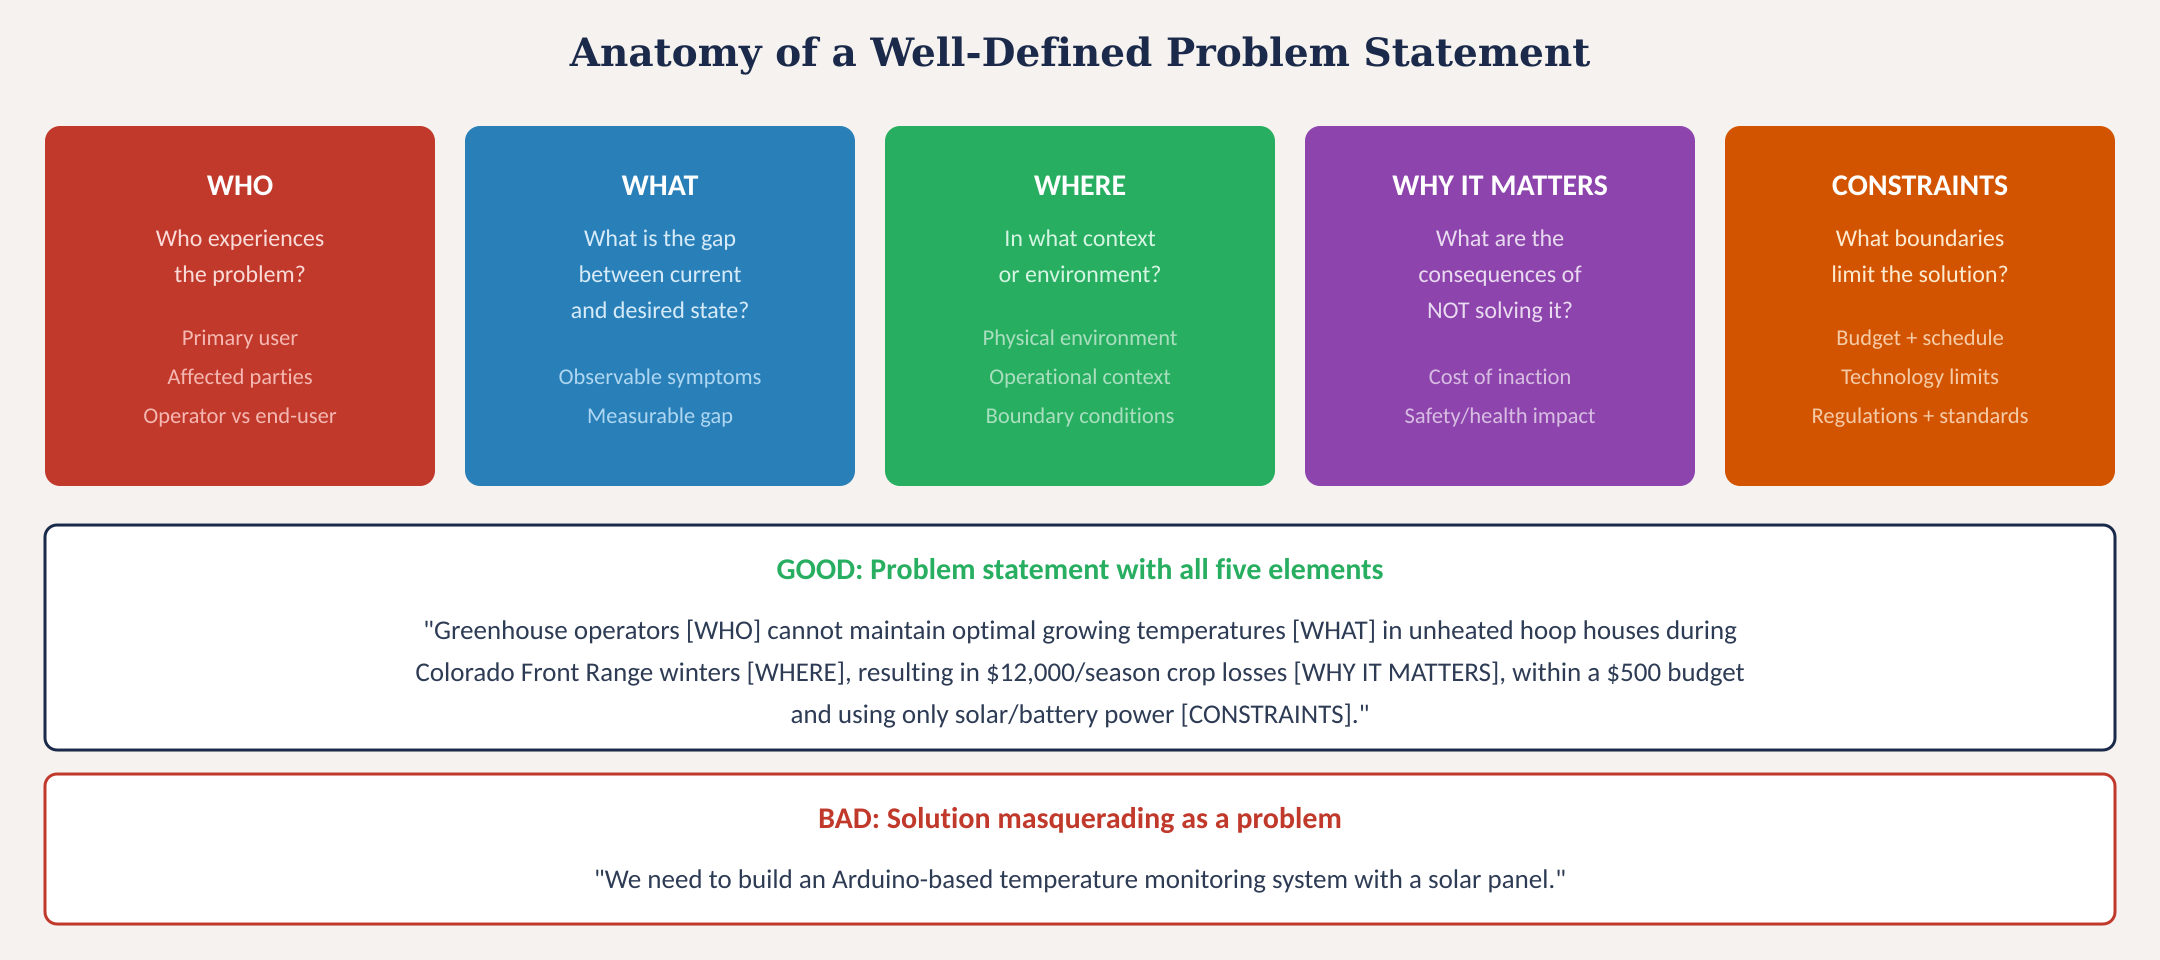
\includegraphics[width=\textwidth]{master_figs/fig_problem_anatomy.png}
\caption{Five-element problem statement framework with good and bad examples.}\label{fig:prob}
\end{figure}

\begin{enumerate}[leftmargin=1.5em]
\item \textbf{WHO}: Who experiences the problem? Be specific about roles and context.
\item \textbf{WHAT}: What is the measurable gap between current and desired states?
\item \textbf{WHERE}: In what physical, operational, or environmental context?
\item \textbf{WHY IT MATTERS}: What are the consequences of not solving it? (Cost, safety, health.)
\item \textbf{CONSTRAINTS}: What boundaries limit the solution? (Budget, schedule, technology, regulations.)
\end{enumerate}

Constraints directly become non-functional requirements. The ``why it matters'' element justifies the project's existence.

\subsection{Scope and Boundaries}
\textbf{Scope} defines what is inside and outside the project. Without it, scope creep expands the project indefinitely. The \textbf{system boundary} distinguishes what you build from what the environment provides. Capture this in a \textbf{context diagram}: your system as a single block with all external interfaces (power, data, user, mechanical, environmental) labeled.

\section{Stakeholder Engagement}
\subsection{Identifying Stakeholders}
A stakeholder is anyone who affects, is affected by, or has an interest in the project. \textbf{Missing a stakeholder = missing requirements = integration surprises.}

\begin{figure}[htbp]\centering
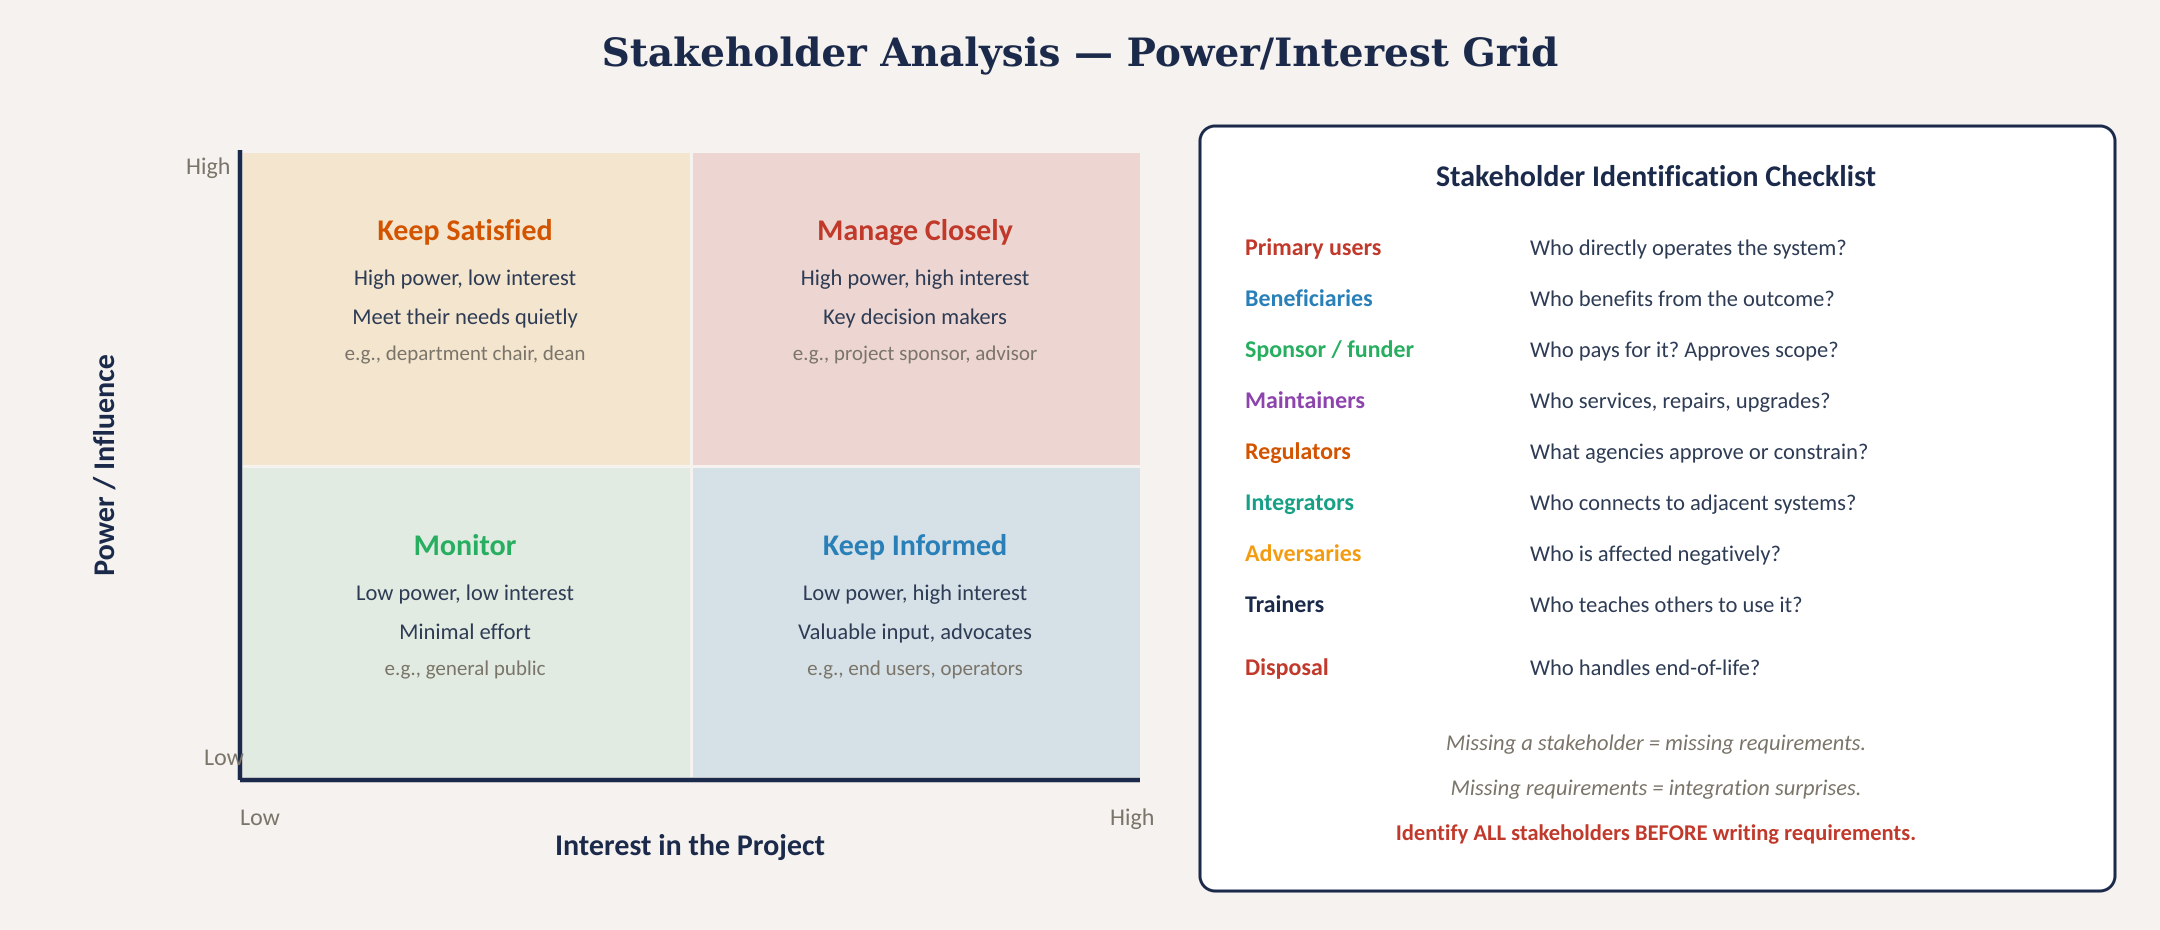
\includegraphics[width=\textwidth]{master_figs/fig_stakeholder_grid.png}
\caption{Power/interest grid with engagement strategies and nine-category identification checklist.}\label{fig:stake}
\end{figure}

\textbf{Nine categories to check}: primary users, beneficiaries, sponsor/funder, maintainers, regulators, integrators (adjacent systems), adversaries, trainers, and disposal handlers. Students consistently miss maintainers, regulators, and adjacent-system owners.

\subsection{The Power/Interest Grid}
Classify each stakeholder by their power (ability to influence the project) and interest (how much they care). Four quadrants with distinct strategies: \textbf{Manage closely} (high power, high interest, key decision makers), \textbf{Keep satisfied} (high power, low interest), \textbf{Keep informed} (low power, high interest, valuable input), \textbf{Monitor} (low power, low interest).

\subsection{Needs Elicitation Techniques}

\begin{figure}[htbp]\centering
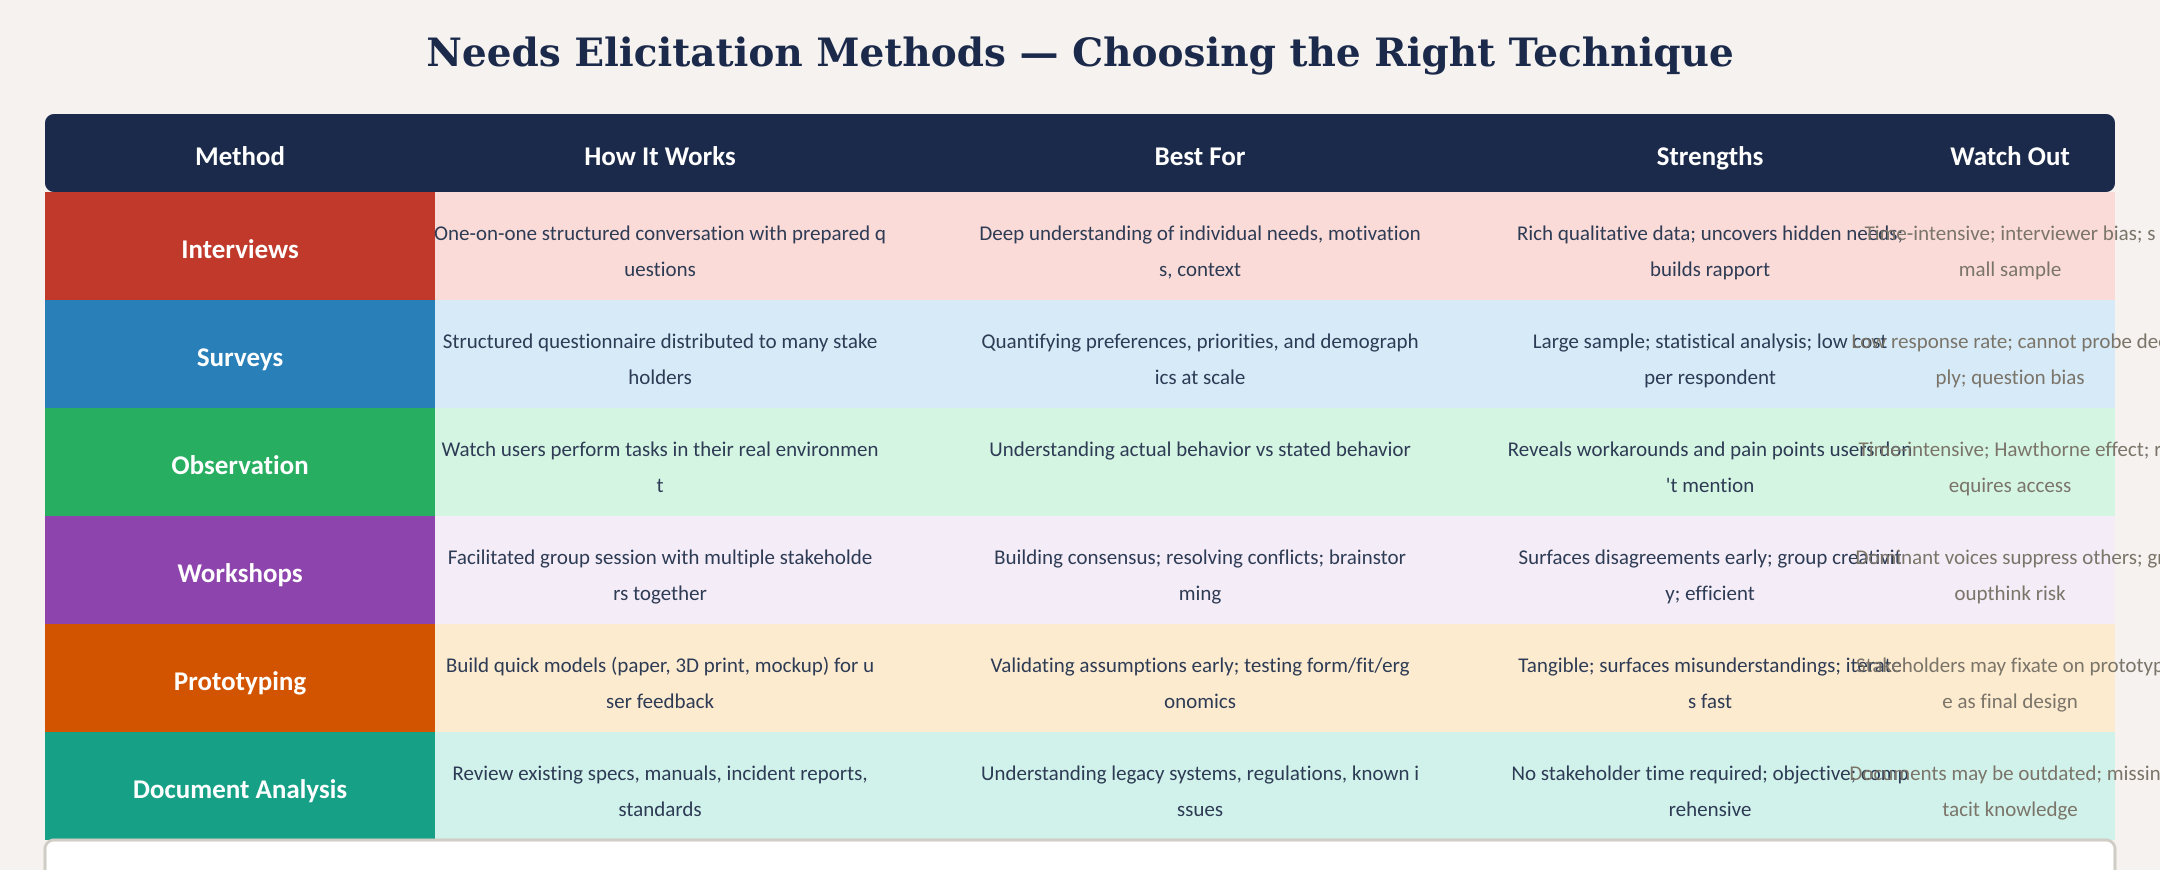
\includegraphics[width=\textwidth]{master_figs/fig_elicitation_methods.png}
\caption{Six elicitation methods with best-use cases, strengths, and watch-outs.}\label{fig:elic}
\end{figure}

Use \textbf{2--3 methods}; single-method elicitation misses needs. Strongest combination for engineering projects: \textbf{interviews} (capture stated needs) + \textbf{observation} (capture unstated needs) + \textbf{prototyping} (validate assumptions).

\begin{tipbox}[The Best Question in Engineering]
End every stakeholder interview with: ``What should I have asked that I didn't?'' This single question catches more missing requirements than any structured technique.
\end{tipbox}

\subsection{Managing Conflicting Needs}
Conflicts are normal. Prioritize using \textbf{MoSCoW}: Must (becomes SHALL), Should (becomes SHOULD), Could (if budget allows), Won't (explicitly excluded). When conflicts are irreconcilable, the sponsor or primary user has final authority, but the decision must be documented.

\subsection{Needs vs.\ Wants}
A \textbf{need} is something without which the system fails its mission, it becomes a SHALL requirement. A \textbf{want} enhances value but the system works without it, it becomes a SHOULD goal pursued only if resources allow. Separate them early.

\section{From Problem to ConOps}
\subsection{Concept of Operations}
The ConOps describes how the system will be used from the stakeholder's perspective, written in \textbf{plain language} (no engineering jargon). Contents: system mission, current situation, operational scenarios (normal, degraded, emergency, maintenance), user roles, environmental conditions, external interfaces, and performance expectations.

The ConOps is the document the stakeholder reviews and approves \textbf{before requirements are written}. Misunderstandings caught here cost minutes; caught in requirements, they cost weeks.

\subsection{Use Cases and Operational Scenarios}
A \textbf{use case} describes a specific user-system interaction to achieve a goal. An \textbf{operational scenario} extends the use case into a realistic narrative with timing, weather, user state, and system state. Scenarios reveal requirements that abstract analysis misses.

\begin{figure}[htbp]\centering
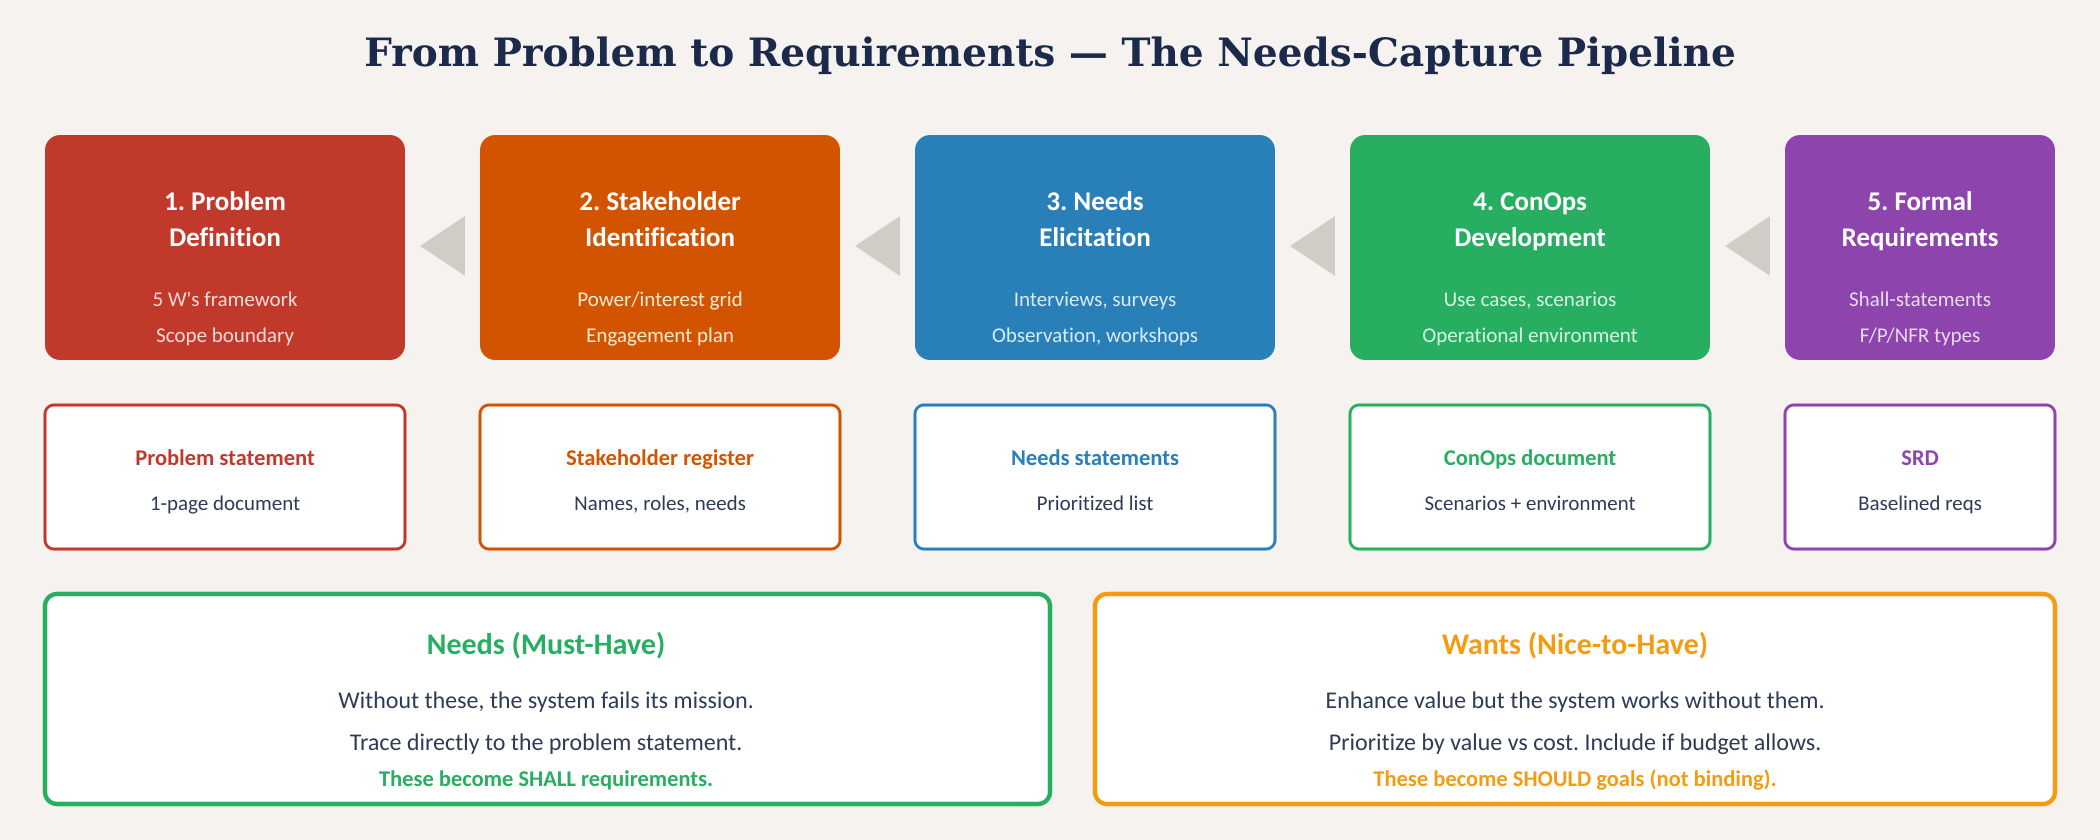
\includegraphics[width=\textwidth]{master_figs/fig_needs_pipeline.png}
\caption{Five-stage needs-capture pipeline from problem to formal requirements with deliverables.}\label{fig:pipe}
\end{figure}


\begin{greenshieldbox}[GreenShield: ConOps to Requirements Mapping]
\textbf{System}: GreenShield. Automated Greenhouse Frost Protection System.

\textbf{ConOps excerpt}: ``When nighttime temperature drops below 3\,\degC{}, the system activates supplemental heating and alerts the operator via SMS. In degraded mode (cellular failure), the system continues autonomous heating control using local logic.''

\textbf{Requirements derived}:
\begin{itemize}[nosep,leftmargin=1.5em]
\item SYS-REQ-001: The system shall monitor air temperature continuously at $\geq$1\,Hz.
\item SYS-REQ-002: The system shall activate the heater when temperature $\leq$ user-defined setpoint (default 3\,\degC{}).
\item SYS-REQ-003: The system shall send an SMS alert within 60\,s of heater activation.
\item SYS-REQ-004: The system shall continue autonomous heating control during communication failure.
\end{itemize}
Every ConOps sentence should map to at least one requirement. If it does not, either the ConOps is too vague or requirements are missing.
\end{greenshieldbox}

\begin{keyconceptbox}[Industry SE Parallels]
\begin{itemize}[nosep,leftmargin=1.5em]
\item \textbf{INCOSE SEH 4th ed.}: Sec.\ 4.1 (Stakeholder Needs and Requirements Definition), Sec.\ 4.2 (System Requirements Definition).
\item \textbf{NASA SP-2016-6105 Rev 2}: Ch.\ 4 (System Design Processes), Sec.\ 4.1 (Stakeholder Expectations Definition).
\item \textbf{IEEE 29148}: Standard for requirements engineering processes.
\end{itemize}
In industry, the ConOps is often a formal deliverable reviewed at a System Requirements Review (SRR), which precedes the Preliminary Design Review. The MoSCoW prioritization method maps to what INCOSE calls ``needs prioritization'' within stakeholder requirements definition.
\end{keyconceptbox}

\section{Artifact Handoff: What Chapter 1 Produces}
\begin{table}[htbp]\centering\small
\begin{tabularx}{\textwidth}{l X l}
\toprule
\textbf{Artifact} & \textbf{Description} & \textbf{Forward Reference} \\
\midrule
Problem Statement & Five-element statement (who/what/where/why/constraints) & Ch.~2 (requirements derivation) \\
Stakeholder Map & Power/interest grid with engagement strategies & Ch.~2, Ch.~4 (validation) \\
Concept of Operations & Plain-language usage scenarios (normal, degraded, emergency) & Ch.~2, Ch.~6 (O\&M) \\
Competitive Analysis & 3--5 competing solutions with gap identification & Ch.~3 (concept generation) \\
Context Diagram & System boundary with external interfaces labeled & Ch.~2 (interface requirements) \\
\bottomrule
\end{tabularx}
\end{table}


\begin{greenshieldbox}[GreenShield: ConOps to Requirements Mapping]
\textbf{System}: GreenShield. Automated Greenhouse Frost Protection System.

\textbf{ConOps excerpt}: ``When nighttime temperature drops below 3\,\degC{}, the system activates supplemental heating and alerts the operator via SMS. In degraded mode (cellular failure), the system continues autonomous control using local logic.''

\textbf{Requirements derived}:
\begin{itemize}[nosep,leftmargin=1.5em]
\item SYS-REQ-001: The system shall monitor air temperature continuously at $\geq$1\,Hz.
\item SYS-REQ-002: The system shall activate the heater when temperature $\leq$ setpoint (default 3\,\degC{}).
\item SYS-REQ-003: The system shall send an SMS alert within 60\,s of heater activation.
\item SYS-REQ-004: The system shall continue autonomous heating control during communication failure.
\end{itemize}
Every ConOps sentence should map to at least one requirement. Unmapped sentences indicate vague ConOps or missing requirements.
\end{greenshieldbox}

\begin{keyconceptbox}[Industry SE Parallels]
\begin{itemize}[nosep,leftmargin=1.5em]
\item \textbf{INCOSE SEH 4th ed.}: \S4.1 Stakeholder Needs Definition, \S4.2 System Requirements Definition.
\item \textbf{NASA SP-2016-6105 Rev~2}: Ch.~4.1 Stakeholder Expectations Definition.
\item \textbf{IEEE 29148}: Requirements engineering processes.
\end{itemize}
\end{keyconceptbox}

\section{Artifact Handoff: What Chapter 1 Produces}
\begin{table}[htbp]\centering\small
\begin{tabularx}{\textwidth}{l X l}
\toprule
\textbf{Artifact} & \textbf{Description} & \textbf{Used In} \\
\midrule
Problem Statement & Five-element statement (who/what/where/why/constraints) & Ch.~2 \\
Stakeholder Map & Power/interest grid with engagement strategies & Ch.~2, 4 \\
Concept of Operations & Plain-language usage scenarios with operational modes & Ch.~2, 6 \\
Competitive Analysis & 3--5 existing solutions with gap identification & Ch.~3 \\
\bottomrule
\end{tabularx}
\end{table}

\section{Stakeholder Analysis Techniques}
\subsection{Stakeholder Identification}
Begin by casting a wide net: who is affected by this product? Beyond the obvious end user, consider: the person who purchases it (may differ from the user), the person who installs and maintains it, the person who disposes of it, regulatory bodies that must approve it, adjacent systems that interact with it, and communities affected by its production and use.

For the GreenShield project, stakeholders typically include: the primary user (the person benefiting from the product's function), the course instructor (who evaluates it against educational objectives), the lab technician (who must store and maintain the prototype), future student teams (who may build on your work), and the environment (affected by material choices and energy consumption).

\subsection{Stakeholder Interviews}
Structured interviews are the most reliable method for understanding stakeholder needs. Prepare 5--8 open-ended questions before the interview:

\emph{``What is the biggest frustration you experience with [current process]?''}

\emph{``Walk me through a typical day where this problem arises.''}

\emph{``If you could change one thing about [existing solution], what would it be?''}

\emph{``What would a perfect solution look like to you?''}

\emph{``How much would you be willing to pay for that solution?''}

Record the responses verbatim; do not paraphrase during the interview. Identify themes across multiple interviews: if three out of five stakeholders mention the same pain point, it is likely a real and significant need.

\subsection{Needs vs.\ Wants vs.\ Constraints}
\textbf{Needs}: requirements that must be met for the product to be useful. ``The device must measure temperature.''

\textbf{Wants}: features that are desired but not essential. ``It would be nice if it displayed the data on a phone app.''

\textbf{Constraints}: limitations imposed by physics, regulations, budget, or the environment. ``It must run on 12\,V battery power because there is no AC outlet at the installation site.''

Distinguishing these three categories during stakeholder analysis prevents over-engineering (spending resources on wants at the expense of needs) and scope creep (adding features that were never required).

\section{Problem Statement Formulation}
A well-written problem statement is the foundation of the entire project. It must be:

\textbf{Specific}: ``Students in MEGN~300 lose 20 minutes per lab session troubleshooting DAQ wiring because the current breadboard setup has unreliable connections.'' Not: ``The lab setup is bad.''

\textbf{Measurable}: include quantified impact. ``The current process wastes \$50{,}000/year in rework costs'' or ``15\% of student groups fail to complete the lab in the allotted time.''

\textbf{Solution-agnostic}: describe the problem, not a solution. ``The building's HVAC system cannot maintain comfortable temperature in Room~201'' (problem). Not: ``Room~201 needs a space heater'' (solution).

\section{Competitive Benchmarking}
Before designing a new product, study what already exists. For each competing product, document:

\textbf{Features}: what does it do? What are its specifications?

\textbf{Price}: what does it cost (purchase, installation, operation)?

\textbf{Strengths}: where does it excel?

\textbf{Weaknesses}: where does it fall short? (These are your opportunities.)

\textbf{Market position}: who buys it? Why?

Organize this information in a competitive comparison matrix. The matrix reveals the gap your product must fill: the unmet need at the intersection of user desire and competitor weakness.
\section{Practice Questions}
\begin{enumerate}[leftmargin=1.5em]
\item Rewrite this solution-as-problem into a proper five-element problem statement: ``We need to design a solar-powered weather station using a Raspberry Pi.''
\item List all stakeholders for a MEGN 301 design project that designs an automated pet feeder for elderly users. Use the nine-category checklist.
\item You interview a greenhouse operator who says ``I need a temperature display.'' Through observation, you notice she checks the display, then walks to the heater and turns it on manually. What is her \emph{actual} need? How does this change the requirements?
\item Classify these stakeholders on a power/interest grid for a campus parking management system: (a) university president, (b) daily commuter student, (c) campus police, (d) city traffic department, (e) disability services office.
\item Write a 1-paragraph ConOps for an automated frost protection system for a small greenhouse, including at least two operational scenarios (normal and degraded mode).

\item \textbf{Market analysis}: existing pet feeders on Amazon range \$30--\$150. Strengths: app connectivity, portion control. Weaknesses: require Wi-Fi (elderly users may lack technical skill), small hoppers (2--3 day capacity), no medication dispensing. Gap: a system designed specifically for elderly users with large-print controls, cellular connectivity (no Wi-Fi setup), and caregiver alerting.

\item \textbf{Customer discovery approach}: interview 3--5 elderly pet owners and 2--3 caregivers. Key questions: ``Show me how you feed your pet today.'' ``What happens when you travel or are hospitalized?'' ``How comfortable are you with smartphone apps?'' Expected insights: manual feeding is a daily routine that provides companionship (do not eliminate it entirely); missed feedings happen during health crises, not routine days; caregivers need alerts, not control.

\item A sponsor wants the system under \$500, the user wants a touchscreen display, and the maintainer wants modular components. These conflict. How do you resolve this using the MoSCoW framework?
\end{enumerate}

\subsection{Answers}
\begin{enumerate}[leftmargin=1.5em]
\item ``Small-farm operators [WHO] lack access to real-time, site-specific weather data [WHAT] at remote agricultural locations without grid power [WHERE], leading to crop management decisions based on regional forecasts that miss micro-climate variations by up to 5\,$^{\circ}$ C [WHY], within a \$300 budget using only renewable power sources [CONSTRAINTS].''
\item Primary users: elderly pet owner (operator). Beneficiaries: the pet; family members who worry remotely. Sponsor: the pet owner or their family. Maintainers: family member or home-care aide who refills food and troubleshoots. Regulators: food-safety standards for pet food storage; electrical safety (UL). Integrators: home Wi-Fi network; smartphone (if app-connected). Adversaries: the pet (may try to defeat the mechanism). Trainers: whoever teaches the elderly user. Disposal: recycling or trash service.
\item Her actual need is automated frost protection, not a temperature display. The display is her current workaround for a lack of automation. The real requirement is: ``The system shall activate the supplemental heater when temperature drops below a user-defined setpoint.'' The display becomes a secondary want, not the primary need. This changes the architecture from a passive monitor to an active control system.
\item (a) University president: high power, low interest $\to$ Keep Satisfied. (b) Commuter student: low power, high interest $\to$ Keep Informed. (c) Campus police: high power, high interest $\to$ Manage Closely (they enforce parking rules). (d) City traffic department: moderate power, low interest $\to$ Keep Satisfied (jurisdiction over surrounding roads). (e) Disability services: moderate power, high interest $\to$ Manage Closely (ADA compliance is non-negotiable).
\item ``The frost protection system monitors greenhouse air temperature continuously. During normal operation, when temperature drops below the user-defined threshold (default 3\,$^{\circ}$ C), the system automatically activates the supplemental heater and sends an alert to the operator's phone. The operator can acknowledge the alert, adjust the setpoint, or override the system remotely. In degraded mode (communication failure), the system continues autonomous control using local logic, activating the heater based on its last-known setpoint and logging events locally until communication is restored. The operator discovers the communication failure on their next manual check or when they notice the absence of the daily status report.''
\item MoSCoW: \textbf{Must}: system cost under \$500 (sponsor constraint; non-negotiable). Modular components for field replacement (maintainer need; essential for long-term usability). \textbf{Should}: visual status display (user need; but a low-cost LCD or LED indicators at \$5 may satisfy the need without a \$50 touchscreen). \textbf{Could}: touchscreen interface (user want; only if budget allows after must-haves). \textbf{Won't}: full-color graphical touchscreen in v1.0. Resolution: the display is a legitimate need but the \emph{touchscreen} is a want. Propose a 2-line LCD (\$3) for v1.0 with a touchscreen upgrade path for v2.0 if the sponsor increases budget.
\end{enumerate}

% ================================================================
\chapter{Value Proposition \& Triple Bottom Line}

\section{Why Value Proposition Matters in Engineering Design}
A technically brilliant product that nobody wants, nobody can afford, or nobody can sustain is a failure. Before investing hundreds of engineering hours in requirements, design, and fabrication, you must answer a fundamental question: \textbf{is this product worth building?} The value proposition framework provides a structured method for answering that question by examining four dimensions: feasibility, desirability, viability, and sustainability. Together, these dimensions ensure that a product concept is not just technically possible, but genuinely valuable to its intended users and stakeholders.

In MEGN~301, your team's GreenShield project must satisfy all four dimensions. A common failure mode in student projects is building something that works (feasible) but that nobody actually needs (not desirable), costs more than the benefit it provides (not viable), or creates environmental harm that outweighs its utility (not sustainable). The value proposition analysis forces you to confront these questions early, when the cost of pivoting is measured in whiteboard sessions rather than scrapped prototypes.

\section{The Four-Dimension Value Framework}

\subsection{Feasibility: Can We Build It?}
Feasibility asks whether the proposed solution is technically achievable within the constraints of the project. It encompasses:

\textbf{Technical feasibility}: do the enabling technologies exist? Can the required performance be achieved with available materials, components, and processes? For the GreenShield project, this means: can the sensors, actuators, and control algorithms deliver the specified performance within the physical constraints (size, weight, power)?

\textbf{Resource feasibility}: does the team have the skills, tools, budget, and time to execute the design? A concept requiring custom ASIC fabrication is technically feasible in industry but infeasible in a one-semester course. Assess honestly: what capabilities does your team have, and what gaps need to be filled through learning, collaboration, or scope reduction?

\textbf{Manufacturing feasibility}: can the product be fabricated with available processes? In MEGN~301, this typically means: 3D printing (FDM, SLA), laser cutting, manual machining, off-the-shelf electronics, and hand soldering. Designs requiring injection molding tooling, CNC 5-axis machining, or custom PCB fabrication with $<$6\,mil traces may be infeasible within the project timeline.

\textbf{Integration feasibility}: can the subsystems be assembled into a working system? This is the most commonly underestimated dimension. Individual subsystems may work perfectly on the bench but fail when integrated due to mechanical interference, electromagnetic compatibility issues, thermal interactions, or software timing conflicts.

\begin{warningbox}[The Feasibility Trap]
Students often confuse ``theoretically possible'' with ``feasible within our constraints.'' A solar-powered autonomous boat is theoretically possible, but designing and building one in 15 weeks with a \$500 budget and no prior experience in waterproofing, marine electronics, or solar power systems is not feasible. Scope your feasibility assessment to your actual resources, not to what a well-funded company could achieve.
\end{warningbox}

\subsection{Desirability: Does Anyone Want It?}
Desirability asks whether the proposed solution addresses a genuine need, want, or pain point for its intended users. It encompasses:

\textbf{User need validation}: have you spoken to actual users (not just imagined their needs)? What problem do they currently face? How do they currently solve it (or work around it)? What would make their life measurably better?

\textbf{User experience}: is the product intuitive to use? Does it fit into the user's existing workflow or environment? A technically superior product with a confusing interface or an inconvenient form factor will not be adopted.

\textbf{Emotional and aesthetic appeal}: beyond functional performance, does the product look and feel appropriate for its context? Industrial equipment should convey ruggedness and reliability. Consumer products should be attractive and approachable. Medical devices should communicate precision and cleanliness.

\textbf{Differentiation}: how is this solution better than existing alternatives? If the answer is ``it isn't, really,'' the product lacks a compelling value proposition regardless of its technical merit.

In MEGN~301, desirability is assessed through stakeholder interviews, user surveys, competitive benchmarking, and design reviews. The Preliminary Design Review (PDR) should include a clear articulation of who the user is, what problem they face, and why your solution is better than the alternatives.

\subsection{Viability: Can It Sustain Itself Economically?}
Viability asks whether the product can be produced and sold at a price that covers costs and generates value. It encompasses:

\textbf{Cost analysis}: what does it cost to produce one unit? Include materials (BOM cost), labor (assembly time $\times$ labor rate), overhead (equipment, facilities, testing), and amortized tooling (mold costs, fixtures). For MEGN~301 prototypes, the relevant question is: does the prototype cost fit within the project budget?

\textbf{Revenue model}: how does the product generate value? For commercial products: unit sales, subscriptions, service contracts, consumables. For internal tools: labor savings, quality improvement, safety enhancement. For the GreenShield project: quantify the value delivered in concrete terms (hours saved, energy reduced, safety incidents prevented).

\textbf{Market sizing}: how many units could realistically be sold? A brilliant niche product with 50 potential customers worldwide may not justify the development investment.

\textbf{Competitive pricing}: what do comparable products cost? Your product must deliver comparable or superior value at a competitive price point, or deliver significantly more value at a premium price.

\subsection{Sustainability: What Are the Long-Term Consequences?}
Sustainability asks whether the product's benefits outweigh its environmental and social costs over its complete life cycle, from raw material extraction through manufacturing, use, and end-of-life disposal. It encompasses:

\textbf{Environmental impact}: what materials are used, and what are their extraction and processing impacts? How much energy does manufacturing consume? What emissions (CO$_2$, VOCs, particulates) does the product generate during use? Can the product be recycled, refurbished, or safely disposed of at end of life?

\textbf{Social impact}: does the product improve or degrade quality of life for its users and the communities affected by its production and disposal? Does the supply chain involve ethical labor practices? Are materials sourced from conflict-free regions?

\textbf{Longevity and durability}: a product that lasts 10 years and is repairable is more sustainable than one that lasts 2 years and must be discarded. Design for durability, repairability, and upgradability reduces the life-cycle environmental footprint per unit of service delivered.

\textbf{Circular economy alignment}: can the product be designed for disassembly, material recovery, and component reuse? Can a take-back program return end-of-life products to the manufacturer for refurbishment or recycling?

\section{The Triple Bottom Line}
The Triple Bottom Line (TBL) framework, introduced by John Elkington in 1994, evaluates organizational and product performance across three dimensions:

\subsection{People (Social)}
The social dimension encompasses the product's impact on all human stakeholders: users, workers, communities, and society at large. Key questions: does the product improve safety, health, or quality of life? Does it create or eliminate jobs? Are workers in the supply chain treated fairly and paid equitably? Does the product respect cultural values and community standards? Is it accessible to people with disabilities?

For the GreenShield project, the social dimension includes: user safety (the product must not create hazards), ergonomics (the product must be comfortable and intuitive to use), and community impact (the product should not generate noise, pollution, or other nuisances for neighbors).

\subsection{Planet (Environmental)}
The environmental dimension encompasses the product's impact on natural systems across its entire life cycle. Key questions: what is the carbon footprint of production and use? What resources (water, energy, rare materials) are consumed? What waste and emissions are generated? Can the product be recycled or biodegraded at end of life?

\textbf{Life Cycle Assessment (LCA)} is the formal methodology for quantifying environmental impacts. A simplified LCA for MEGN~301 projects should consider: (1) materials -- mass and type (metals, plastics, electronics, batteries), (2) manufacturing energy (3D printing, machining, soldering), (3) use-phase energy consumption (if powered), (4) transportation (shipping weight and distance), and (5) end-of-life fate (landfill, recycling, hazardous waste).

\begin{tipbox}[Quick Environmental Impact Estimation]
For a rough LCA in MEGN~301: (1)~Sum the mass of each material category. (2)~Multiply by the embodied energy factor: aluminum $\approx 170$\,MJ/kg, steel $\approx 25$\,MJ/kg, ABS plastic $\approx 95$\,MJ/kg, copper (PCB) $\approx 60$\,MJ/kg, lithium battery $\approx 400$\,MJ/kg. (3)~Sum to get total embodied energy. (4)~Add use-phase energy ($P_{\text{watts}} \times t_{\text{hours}} \times 0.0036$\,MJ/Wh $\times$ lifetime years). (5)~Compare to the energy saved or the environmental benefit delivered by the product.
\end{tipbox}

\subsection{Profit (Economic)}
The economic dimension ensures the product is financially sustainable. A product that loses money on every unit sold, no matter how socially and environmentally beneficial, cannot persist. The economic dimension includes: unit manufacturing cost, expected selling price, gross margin ($\geq$40\% for hardware products to cover overhead, distribution, and warranty), development cost recovery (break-even volume), and total cost of ownership for the user (purchase price + operating costs + maintenance + disposal).

\section{Applying TBL to the GreenShield Project}
Every GreenShield project should include a TBL assessment in the Preliminary Design Review:

\textbf{People}: who benefits? Who is affected? What safety considerations exist? How does the product improve the user's daily experience?

\textbf{Planet}: what is the estimated embodied energy? What is the use-phase energy consumption? What materials require special disposal (batteries, electronics)? Can the product be disassembled for recycling?

\textbf{Profit}: what is the estimated BOM cost? What would a realistic selling price be? How many units would need to be sold to recover the development investment? What is the user's return on investment (cost savings or productivity improvement)?

The TBL analysis does not require precise numbers at the concept stage. Order-of-magnitude estimates are sufficient to identify show-stoppers (e.g., a product that costs \$500 to build but competes with \$20 alternatives, or a product whose battery contains 5\,kg of lithium that cannot be recycled).

\begin{greenshieldbox}[GreenShield Template: Value Proposition Summary]
Include in your PDR package:
\begin{itemize}[nosep,leftmargin=1.5em]
\item \textbf{User}: Who is the primary user? What is their unmet need?
\item \textbf{Solution}: What does our product do, in one sentence?
\item \textbf{Feasibility}: What is the highest-risk technical element? How will we mitigate it?
\item \textbf{Desirability}: What evidence do we have that users want this? (Interview quotes, survey data, competitive gap.)
\item \textbf{Viability}: Estimated BOM cost vs.\ target price. Estimated market size.
\item \textbf{Sustainability}: Estimated embodied energy. End-of-life plan. Key environmental risks.
\item \textbf{TBL Summary}: One sentence each for People, Planet, Profit impact.
\end{itemize}
\end{greenshieldbox}

\section{Value Proposition Canvas}
The Value Proposition Canvas (Osterwalder \& Pigneur) is a visual tool that maps the product's features to the customer's needs:

\textbf{Customer Profile} (right side): Jobs (what the customer is trying to accomplish), Pains (obstacles, risks, frustrations), Gains (desired outcomes, benefits, aspirations).

\textbf{Value Map} (left side): Products \& Services (what you offer), Pain Relievers (how your product addresses each pain), Gain Creators (how your product delivers each gain).

A strong value proposition achieves \textbf{fit}: every significant customer pain is addressed by a pain reliever, and every important gain is delivered by a gain creator. Unaddressed pains represent risks; undelivered gains represent missed opportunities.

\section{Stakeholder Value Mapping}
Different stakeholders derive different value from the same product. A comprehensive value proposition addresses each stakeholder's perspective:

\textbf{End user}: functional value (does it solve my problem?), experiential value (is it pleasant to use?), and economic value (does it save me money or time?).

\textbf{Buyer} (may be different from user): economic value (ROI, payback period), risk reduction (warranty, reliability, vendor stability), and compliance value (meets regulatory requirements, company standards).

\textbf{Installer/maintainer}: ease of installation, ease of maintenance, availability of spare parts, quality of documentation.

\textbf{Society}: environmental impact, safety, job creation/displacement, resource consumption.

For the GreenShield project, map each stakeholder's needs to specific product features and quantify the value delivered where possible.

\section{Business Model Canvas Integration}
The Value Proposition Canvas fits within the larger Business Model Canvas (BMC), which describes the complete business logic:

\textbf{Key Partners}: who supplies critical components, expertise, or distribution? For a GreenShield product: PCB fabricators, sensor suppliers, cloud service providers.

\textbf{Key Activities}: what must the team do to deliver the value proposition? Design, fabrication, testing, user support.

\textbf{Key Resources}: what assets are needed? Engineering talent, lab equipment, funding, IP.

\textbf{Cost Structure}: what are the major costs? BOM, labor, testing equipment, certification.

\textbf{Revenue Streams}: how does the product generate income? Unit sales, service contracts, data subscriptions, licensing.

While MEGN~301 is not a business course, understanding the BMC ensures your technical design fits within a viable business context. A product that cannot be profitably produced, distributed, and supported will not survive regardless of its technical merit.

\section{Competitive Analysis Framework}
\subsection{Direct Competitors}
Products that solve the same problem in the same way. Compare feature-by-feature: performance, price, size, weight, reliability, user experience. Identify where your product is superior (the competitive advantage) and where it lags (the competitive disadvantage that must be accepted or mitigated).

\subsection{Indirect Competitors}
Products that solve the same problem in a different way, or products that make the problem less important. For a portable water purifier: indirect competitors include bottled water, municipal treatment upgrades, and UV sterilization pens. Understanding indirect competitors reveals the true competitive landscape and the user's switching cost.

\subsection{Non-Consumption}
The most powerful competitor is often ``doing nothing.'' If the user is currently tolerating the problem without any solution, your product must overcome the inertia of non-consumption. The value proposition must be compelling enough that the user is willing to change their behavior, invest money, and learn a new system.

\section{Quantifying Value: The Business Case}
For B2B (business-to-business) products, the value proposition must be quantified financially:

\textbf{Cost savings}: ``Our sensor reduces calibration time from 2 hours to 15 minutes. At \$75/hour for a technician with 50 sensors calibrated annually: savings $= 50 \times 1.75 \times \$75 = \$6{,}563$/year.''

\textbf{Revenue increase}: ``Our quality monitoring system reduces defect rates from 2\% to 0.5\%, recovering \$15{,}000/year in scrapped product.''

\textbf{Risk reduction}: ``Our safety interlock prevents the failure mode that caused \$200{,}000 in damage last year. Even at 10\% probability: expected savings $= \$20{,}000$/year.''

\textbf{Payback period}: the time for cumulative savings to exceed the product cost. For B2B products: $<$2 years is attractive, $<$1 year is compelling, $>$3 years is difficult to justify.

For B2C (business-to-consumer) products, value is often experiential rather than financial, and quantification is harder. Use: willingness-to-pay surveys, comparable product pricing, and customer satisfaction metrics.
\section{Practice Questions}
\begin{enumerate}[leftmargin=1.5em]
\item Your team proposes a solar-powered phone charging station for campus bus stops. Evaluate feasibility, desirability, viability, and sustainability. Identify the highest-risk dimension and propose a mitigation strategy.
\item A GreenShield team's product costs \$120 in materials and takes 8 hours to assemble. The product saves the user approximately \$15/month in energy costs. Calculate the payback period. Is this viable for a consumer market? For an industrial market?
\item Conduct a simplified TBL assessment for a battery-powered portable fan. List two considerations for each dimension (People, Planet, Profit).
\item Explain why a product can be feasible and desirable but not viable. Give a specific example from consumer electronics.
\item Your product uses a 5000\,mAh lithium-polymer battery. Research the environmental impact of lithium mining and battery disposal. Propose a design change that would improve the product's sustainability score.
\end{enumerate}

\subsection{Answers}
\begin{enumerate}[leftmargin=1.5em]
\item Feasibility: solar panel + charge controller + USB outlets is proven technology; risk is weather variability and vandalism. Desirability: students waiting at bus stops often have low phone battery; validated by informal survey. Viability: \$200 BOM, no revenue model unless campus funds it; viable as a university sustainability project, not as a commercial product. Sustainability: solar energy is renewable; battery and electronics require recycling; aluminum enclosure is recyclable. Highest risk: viability (no clear revenue); mitigation: frame as a grant-funded campus improvement, not a commercial product.
\item Payback $= \$120/\$15 = 8$ months. For consumer: borderline viable (consumers prefer $<$6-month payback for energy products). For industrial: excellent (industrial buyers accept 1--3 year payback). Viability depends on the target market, not just the technology.
\item People: (+) provides comfort in hot environments, ($-$) battery creates disposal hazard. Planet: (+) reduces need for large HVAC, ($-$) battery and motor require mining and energy-intensive manufacturing. Profit: (+) low BOM (\$15--30), ($-$) intense competition from established brands drives margins below 20\%.
\item A product can be technically buildable (feasible) and users may want it (desirable), but if it costs more to produce than customers will pay, it is not viable. Example: modular smartphones (Project Ara) were technically feasible and highly desired by tech enthusiasts, but the modular design added \$100+ to manufacturing cost, making the price uncompetitive with integrated designs.
\item LiPo batteries contain lithium (from brine extraction in Chile/Argentina, high water consumption), cobalt (from DRC, ethical concerns), and electrolytes (flammable, toxic). Design change: reduce battery capacity to 2500\,mAh (sufficient for the application) and design the enclosure for easy battery replacement and return. Add a QR code linking to a battery recycling drop-off locator. Switch from cobalt-based to lithium iron phosphate (LFP) chemistry, which is cobalt-free and more recyclable.
\end{enumerate}
\chapter{Writing Requirements \& Defining Architecture}

\vspace{1em}


\vspace{1em}

\section{Writing Requirements}
\subsection{The System Design Requirements Document (SDRD)}
The SDRD is the single authoritative document that captures all system-level requirements, their rationale, traceability, and verification methods. Standard structure:
\begin{enumerate}[nosep,leftmargin=1.5em]
\item \textbf{Introduction}: system overview, scope, applicable documents.
\item \textbf{System Description}: ConOps summary, system boundary, external interfaces.
\item \textbf{Requirements}: organized by functional, performance, and non-functional categories. Each includes: unique ID, shall-statement, rationale, parent traceability, verification method (T/A/I/D).
\item \textbf{Traceability Matrix}: forward (need $\to$ requirement) and backward (requirement $\to$ need).
\item \textbf{Verification Plan Summary}: method assignments and planned test phases.
\end{enumerate}
The SDRD is a living document; baselined at PDR and updated under change control through CDR and FDR.


\subsection{The System Design Requirements Document (SDRD)}
The SDRD is the single authoritative document capturing all system-level requirements, their rationale, traceability, and verification methods. Structure:
\begin{enumerate}[nosep,leftmargin=1.5em]
\item \textbf{Introduction}: system overview, scope, applicable documents.
\item \textbf{System Description}: ConOps summary, system boundary, external interfaces.
\item \textbf{Requirements}: organized by functional, performance, and non-functional categories. Each entry: unique ID, shall-statement, rationale, parent traceability, verification method (T/A/I/D).
\item \textbf{Traceability Matrix}: forward (need $\to$ requirement) and backward (requirement $\to$ need).
\item \textbf{Verification Plan Summary}: method assignments and planned test phases.
\end{enumerate}
The SDRD is baselined at PDR and updated under change control through CDR and FDR.

\subsection{What Is a Requirement?}
A requirement is a formal statement of a capability or constraint the system must satisfy. It uses the word \textbf{shall} to indicate mandatory compliance. ``The system \emph{shall} measure ambient temperature'' is a requirement. ``Should'' and ``will'' are non-binding.

A well-formed requirement has: (1) a unique ID (SYS-REQ-042) for traceability, (2) a single shall-statement with one testable condition, (3) measurable acceptance criteria with units and tolerance, (4) a rationale explaining why it exists, and (5) a verification method (Test, Analysis, Inspection, or Demonstration).

\begin{warningbox}[Common Failures]
\textbf{Vague}: ``shall be fast.'' \textbf{Compound}: ``shall measure AND display.'' \textbf{Untestable}: ``shall be user-friendly.'' \textbf{Gold-plated}: ``shall use an Arduino'' (specifies implementation, not need). Each failure produces downstream rework.
\end{warningbox}

\subsection{Requirement Types}
\begin{itemize}[leftmargin=1.5em]
\item \textbf{Functional}: What the system shall \emph{do}. Actions: sense, compute, transmit, actuate, display. ``The system shall measure ambient temperature.''
\item \textbf{Performance}: How \emph{well} it does it. Quantitative criteria. ``\ldots with accuracy of $\pm 0.5$\,$^{\circ}$ C over $-20$ to $+60$\,$^{\circ}$ C at $\geq$1\,Hz.'' A functional requirement without a paired performance requirement is incomplete.
\item \textbf{Non-Functional (NFR)}: Constraints on \emph{how} it is built. Environmental (``operate at $-20$ to $+60$\,$^{\circ}$ C''), regulatory (``comply with FCC Part 15''), material (``RoHS-compliant''), reliability (``$\geq$1000 hrs MTBF''), interface (``CAN 2.0B'').
\end{itemize}

\subsection{Requirements Hierarchy and Traceability}
Requirements decompose top-down: stakeholder needs $\to$ system requirements $\to$ subsystem requirements $\to$ component specifications. Each level adds detail. Every child requirement traces to a parent (backward traceability). Every parent is decomposed into children (forward traceability). An orphan requirement has no justification; an undecomposed requirement has no implementation.

\begin{figure}[htbp]\centering
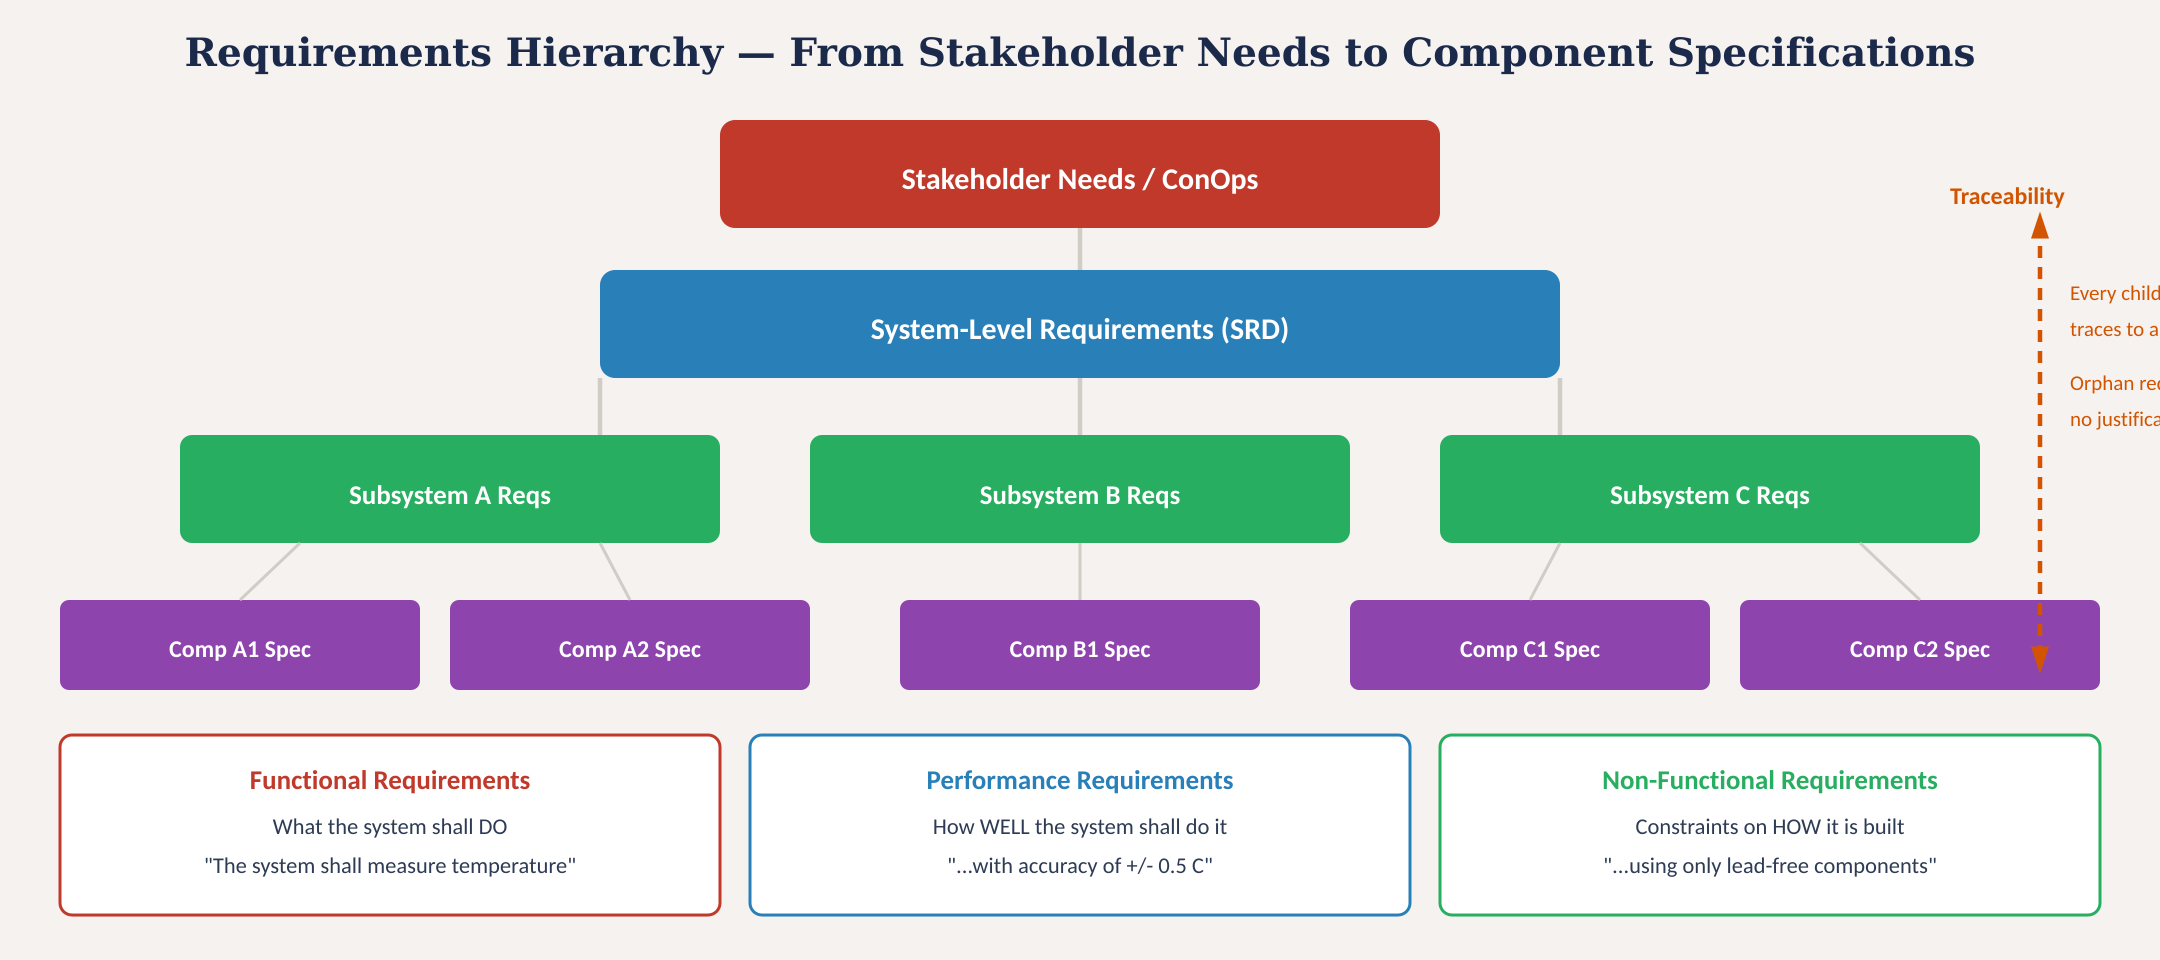
\includegraphics[width=\textwidth]{master_figs/fig_req_hierarchy.png}
\caption{Requirements hierarchy from stakeholder needs through system, subsystem, and component levels with traceability and three requirement types.}\label{fig:hier}
\end{figure}


\subsection{The Requirements Quality Checklist}
Before baselining any requirement, verify it passes all seven tests:
\begin{enumerate}[nosep,leftmargin=1.5em]
\item \textbf{Necessary}: does it trace to a stakeholder need? (No gold-plating.)
\item \textbf{Unambiguous}: can it be interpreted only one way?
\item \textbf{Complete}: does it include all conditions (range, tolerance, units)?
\item \textbf{Consistent}: does it conflict with any other requirement?
\item \textbf{Verifiable}: can you write a test procedure for it right now?
\item \textbf{Traceable}: does it have a unique ID and parent link?
\item \textbf{Implementation-free}: does it specify WHAT, not HOW?
\end{enumerate}
A requirement that fails any test must be rewritten before PDR.

\subsection{Writing Good Requirements: Five Rules}
\begin{enumerate}[leftmargin=1.5em]
\item \textbf{One shall per requirement}: compound requirements are untestable.
\item \textbf{Quantitative criteria}: numbers, units, tolerance. ``Fast'' is not a requirement.
\item \textbf{Testable as written}: if you cannot envision a test procedure, rewrite.
\item \textbf{Implementation-free}: state WHAT, not HOW. ``$\geq$12 analog inputs'' not ``use Arduino Mega.''
\item \textbf{Include rationale}: WHY does this requirement exist? Prevents zombie requirements.
\end{enumerate}

\section{Defining Architecture}
\subsection{Functional Decomposition}
Define WHAT the system must do (functions) before deciding HOW (physical components). Break the mission into primary functions, sub-functions, and leaf functions. Each leaf maps to a physical component. Use verb-noun naming: Sense Temperature, Process Data, Provide Power.

\begin{figure}[htbp]\centering
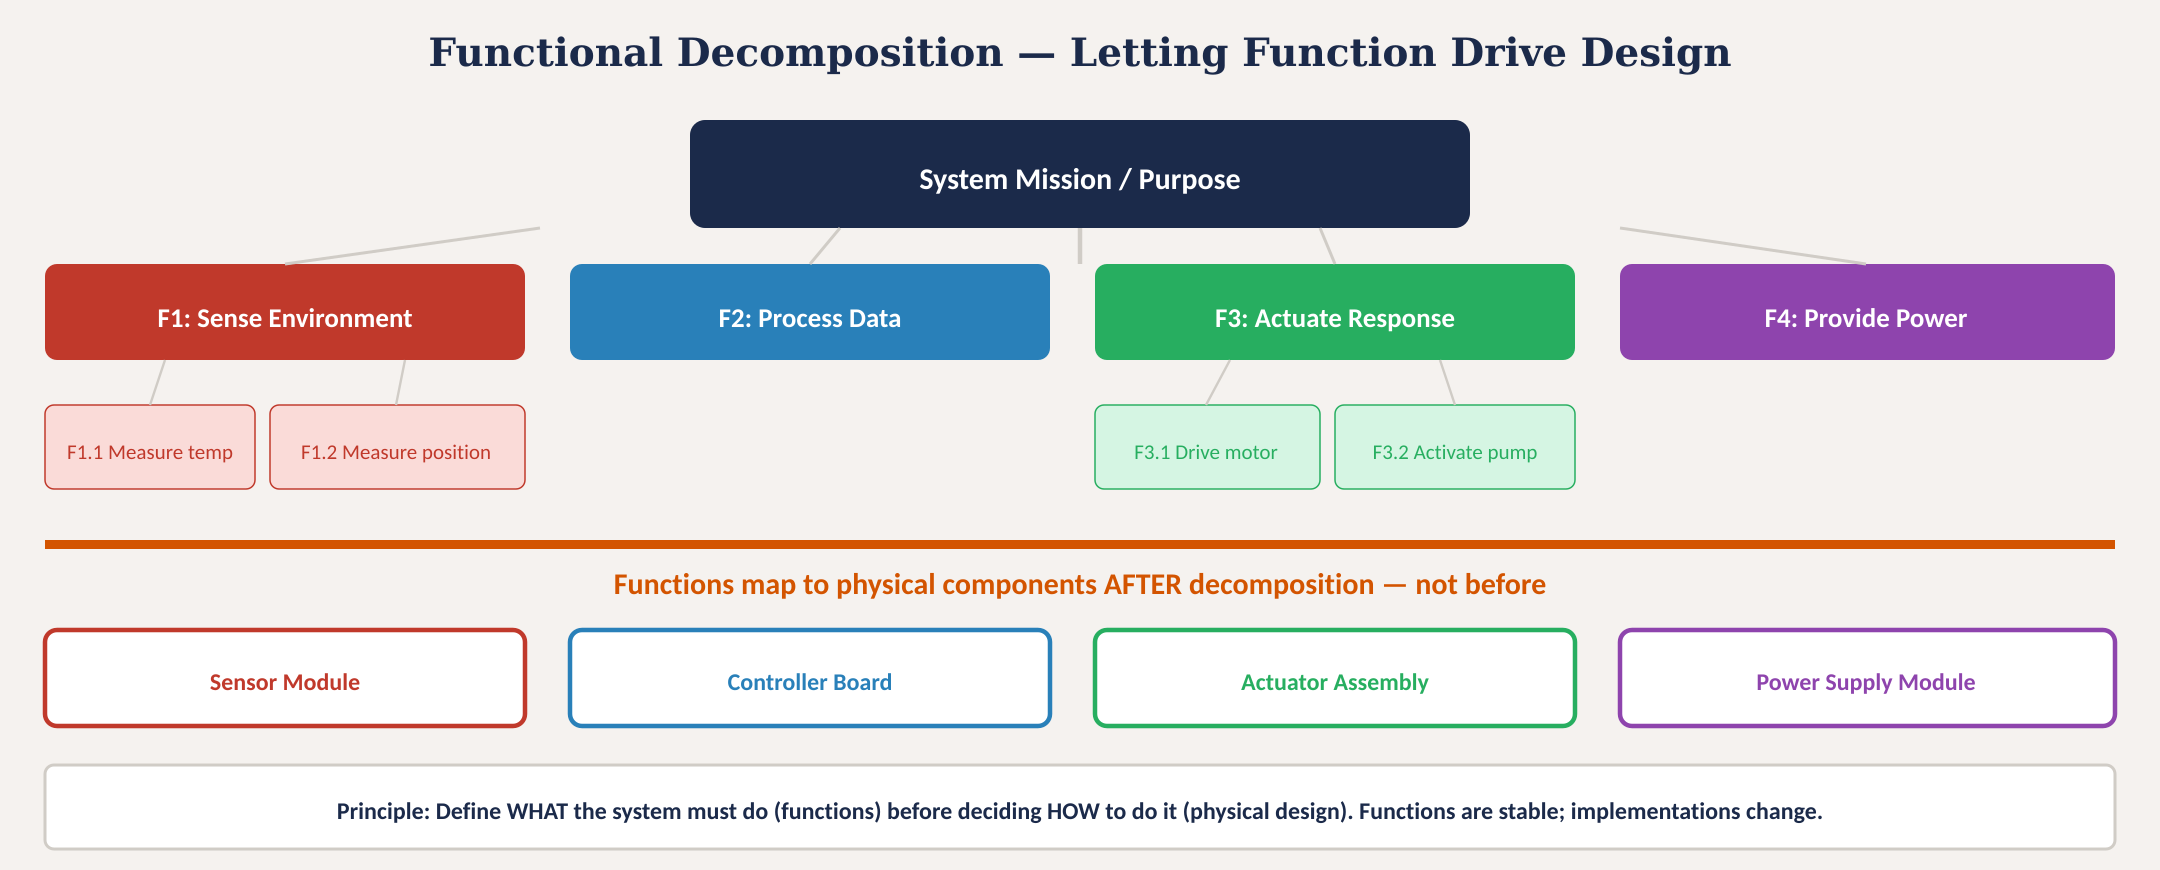
\includegraphics[width=\textwidth]{master_figs/fig_functional_decomp.png}
\caption{Functional decomposition: functions defined before physical allocation. Functions are stable; implementations change.}\label{fig:func}
\end{figure}


\subsection{From Functions to Architecture Blocks}
Functional decomposition produces a tree of functions (verb-noun). Architecture allocation maps each leaf function to a physical module. This mapping is one-to-many (one function may require multiple modules) and many-to-one (one module may implement multiple functions). Document this in an \textbf{allocation matrix}: rows = functions, columns = physical modules, cells = primary/supporting role.

The allocation matrix reveals integration complexity: modules that implement many functions are high-risk single points of failure.


\subsection{From Functions to Architecture Blocks}
Functional decomposition produces a tree of functions (verb-noun pairs). Architecture allocation maps each leaf function to a physical module. This mapping is one-to-many (one function may require multiple modules) and many-to-one (one module may implement multiple functions). Document this in an \textbf{allocation matrix}: rows = functions, columns = physical modules, cells = primary/supporting role.

The allocation matrix reveals integration complexity: modules implementing many functions are high-risk. Modules sharing functions require careful interface definition.

\subsection{Interface Definition}
Once functions map to modules, define interfaces between them with Interface Control Documents (ICDs): what crosses the boundary (signals, power, data), in what format (protocols, voltage levels), with what constraints (bandwidth, latency).


\begin{tipbox}[Start Your FMEA During Architecture: Not at FDR]
Failure Mode and Effects Analysis (FMEA) is most valuable \emph{before} hardware is ordered. As you allocate functions to physical modules (this chapter), immediately ask: ``What happens if this module fails?'' Chapter~3 provides the full FMEA framework and a worked GreenShield example. Performing FMEA during architecture (Chapters~2--3) enables you to design out critical failure modes. Waiting until O\&M (Chapter~6) turns FMEA into an autopsy on a failed project.
\end{tipbox}

\subsection{Architecture Patterns}
\textbf{Centralized}: one controller. Simple but single point of failure. \textbf{Distributed}: multiple controllers on a bus (CAN, I$^2$C). More robust, enables parallel development. \textbf{Hierarchical}: layered control. Choose based on reliability, complexity, and team structure.


\subsection{Requirements--Architecture Iteration}
Requirements and architecture co-evolve. Initial requirements drive a candidate architecture. That architecture reveals implementation constraints (weight, power, thermal) that feed back as new requirements or modified performance targets. This iteration is normal and healthy, but must be \textbf{documented}. Each iteration produces a revised SDRD version with change rationale.

Convergence test: when two consecutive iterations change fewer than 5\% of requirements, the design is stable enough to baseline at PDR.

\section{Environmental and Regulatory Constraints}
Every system operates in an environment that imposes constraints. Systematically address:
\begin{itemize}[nosep,leftmargin=1.5em]
\item \textbf{Temperature}: operating range, storage range, thermal shock.
\item \textbf{Moisture/IP rating}: splash (IPX4), rain (IPX5), submersion (IPX7/8).
\item \textbf{Vibration/shock}: transport, operational, handling drop.
\item \textbf{EMC}: FCC Part 15 Class B (residential), IEC 61000 (EU).
\item \textbf{Safety}: UL/CSA/CE marking, OSHA regulations, university lab safety policies.
\item \textbf{Materials}: RoHS compliance, California Prop 65, food-contact (FDA 21 CFR).
\end{itemize}


\subsection{Requirements--Architecture Iteration}
Requirements and architecture co-evolve. Initial requirements drive a candidate architecture; that architecture reveals implementation constraints (weight, power, thermal) that feed back as new requirements or modified targets. This iteration is normal, but must be \textbf{documented}. Each iteration produces a revised SDRD version with change rationale.

\textbf{Convergence test}: when two consecutive iterations change fewer than 5\% of requirements, the design is stable enough to baseline at PDR.

\section{Environmental and Regulatory Constraints}
Every system operates in an environment that imposes constraints. Systematically address:
\begin{itemize}[nosep,leftmargin=1.5em]
\item \textbf{Temperature}: operating range, storage range, thermal shock.
\item \textbf{Moisture/IP}: splash (IPX4), rain (IPX5), submersion (IPX7/8).
\item \textbf{Vibration/shock}: transport, operational, handling drop height.
\item \textbf{EMC}: FCC Part 15 Class B (residential), IEC 61000 (EU).
\item \textbf{Safety}: UL/CSA/CE marking, OSHA, university lab safety policies.
\item \textbf{Materials}: RoHS compliance, California Prop 65, food-contact (FDA 21~CFR).
\end{itemize}

\section{Trade Studies and Decision Making}
\subsection{The Trade Study Process}
\begin{enumerate}[leftmargin=1.5em]
\item Define the decision and evaluation criteria (derived from requirements). Weight criteria (sum to 1.0).
\item Identify 3--5 viable candidates. No straw-men.
\item Rate each option against each criterion using data, not preference.
\item Score (raw $\times$ weight), sum, select. Check sensitivity: if $\pm$0.05 weight change flips the winner, investigate further.
\item Document everything: matrix, data sources, weight rationale, dissenting opinions.
\end{enumerate}

\subsection{Pugh Matrix vs.\ Weighted Decision Matrix}
\textbf{Pugh (screening)}: rate options as $+$, S, $-$ against a datum. Fast. No weights. Eliminates clearly inferior options. \textbf{Weighted matrix (selection)}: numerical ratings $\times$ weights. Rigorous, quantitative, traceable. Best practice: Pugh to screen $\to$ weighted matrix to select.

\begin{figure}[htbp]\centering
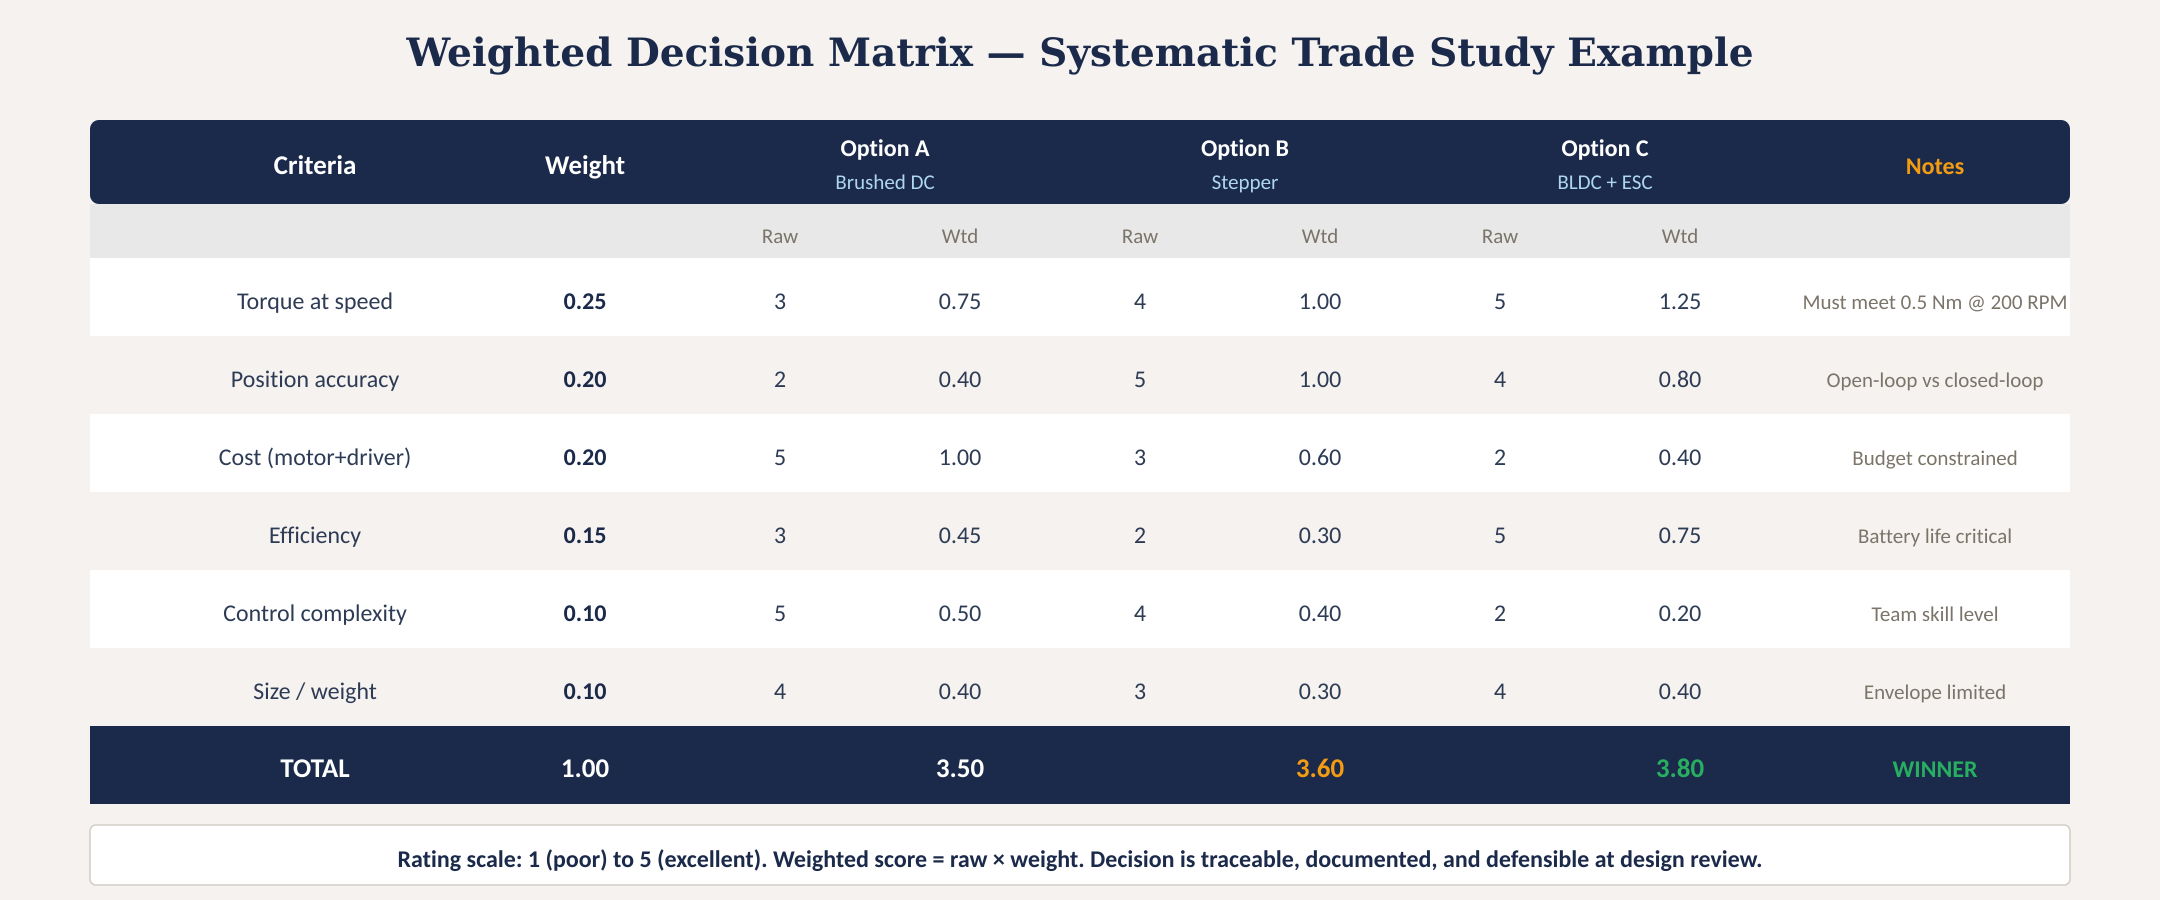
\includegraphics[width=\textwidth]{master_figs/fig_decision_matrix.png}
\caption{Weighted decision matrix example: motor selection with six criteria, three options.}\label{fig:matrix}
\end{figure}


\subsection{Worked Example: MCU Trade Study}
\textbf{Decision}: Select an MCU platform for a battery-powered environmental sensor node.

\begin{table}[htbp]\centering\small
\begin{tabularx}{\textwidth}{l c c c c}
\toprule
\textbf{Criterion (Weight)} & \textbf{ESP32} & \textbf{STM32L4} & \textbf{ATmega328P} \\
\midrule
Power consumption (0.25) & 3 (0.75) & 5 (1.25) & 4 (1.00) \\
Analog channels (0.20) & 5 (1.00) & 4 (0.80) & 4 (0.80) \\
Cost (0.20) & 5 (1.00) & 3 (0.60) & 5 (1.00) \\
Flash/RAM (0.15) & 5 (0.75) & 5 (0.75) & 2 (0.30) \\
Ecosystem (0.10) & 5 (0.50) & 3 (0.30) & 5 (0.50) \\
Wi-Fi/BLE (0.10) & 5 (0.50) & 1 (0.10) & 1 (0.10) \\
\midrule
\textbf{Total} & \textbf{4.50} & \textbf{3.80} & \textbf{3.70} \\
\bottomrule
\end{tabularx}
\caption{MCU trade study for battery-powered sensor node.}
\end{table}

\textbf{Sensitivity check}: If ``Power consumption'' weight increases from 0.25 to 0.30 (taking 0.05 from Wi-Fi), STM32L4 total rises to 4.05 and ESP32 drops to 4.40; winner unchanged. Selection is robust.

\textbf{Decision}: ESP32. Despite higher power draw, the built-in Wi-Fi eliminates a separate module (\$8 saved, one fewer interface, one fewer failure mode). For battery life, use deep sleep aggressively (Section~12.4).

\section{Requirements-to-Architecture Flow}
\begin{figure}[htbp]\centering
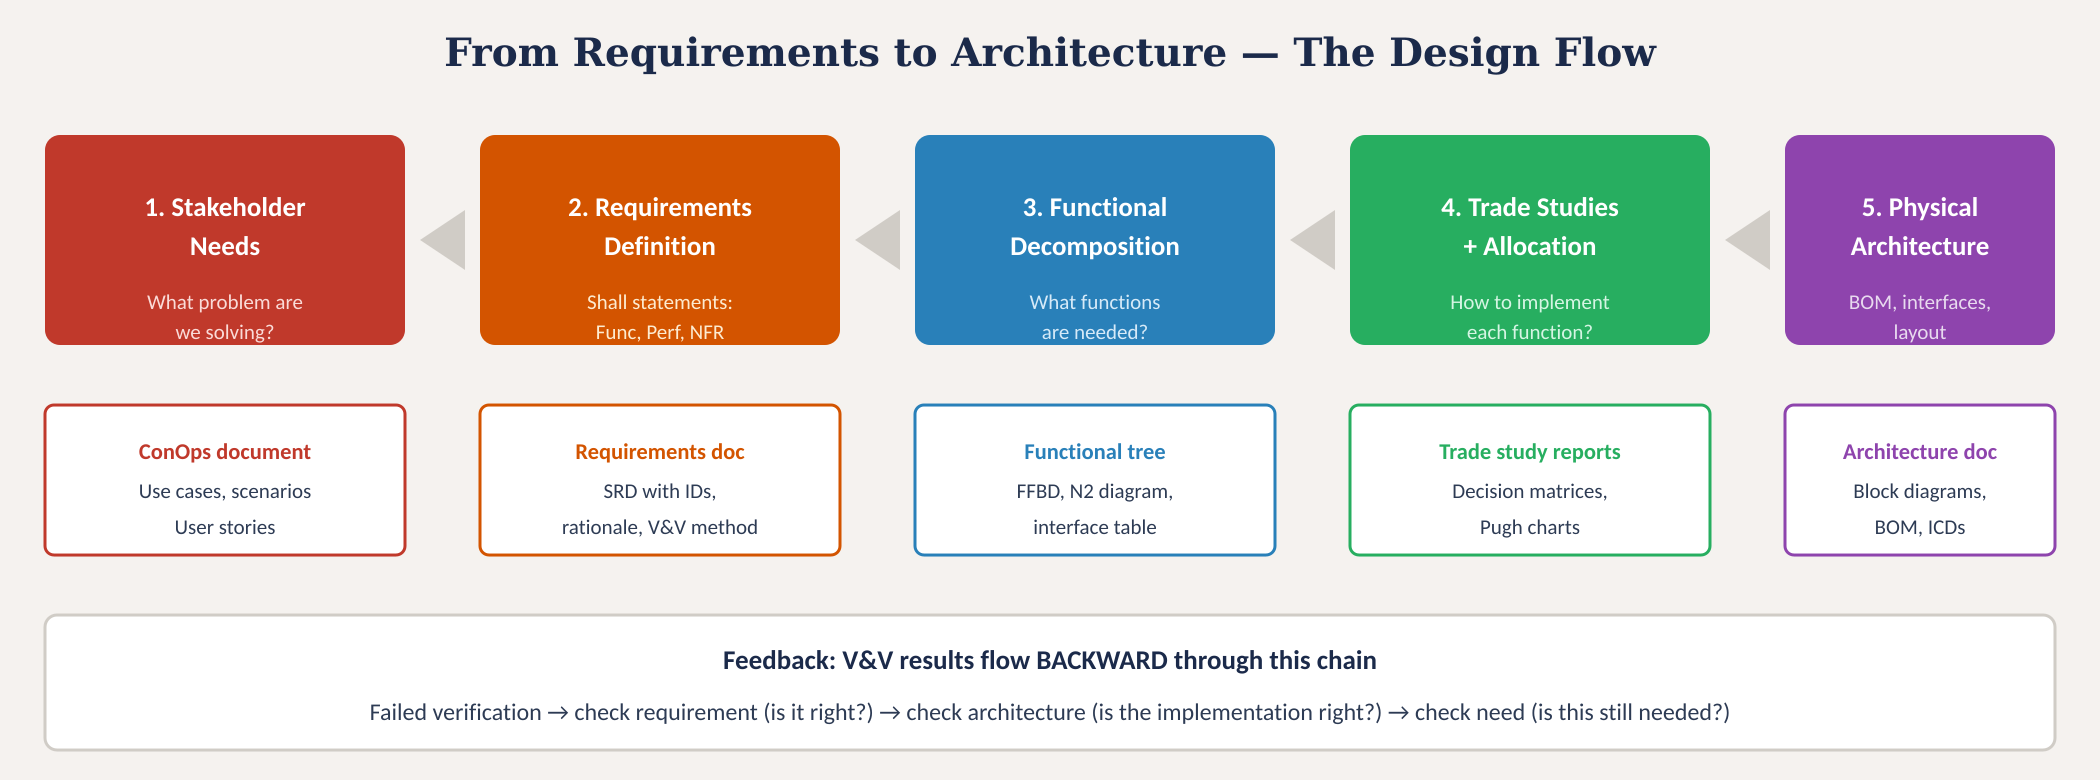
\includegraphics[width=\textwidth]{master_figs/fig_design_flow.png}
\caption{Five-stage design flow: stakeholder needs $\to$ requirements $\to$ functional decomposition $\to$ trade studies $\to$ architecture.}\label{fig:flow}
\end{figure}

The five stages produce specific deliverables: ConOps, requirements document, functional tree, trade study reports, and architecture document (block diagrams + BOM + ICDs). V\&V results feed backward through the chain when failures occur.


\begin{greenshieldbox}[GreenShield: Functional Decomposition]
\textbf{Top-level function}: Protect greenhouse crops from frost damage.

Decomposition:
\begin{itemize}[nosep,leftmargin=1.5em]
\item \textbf{Sense Environment} $\to$ Measure Air Temp, Measure Soil Temp, Detect Heater Status
\item \textbf{Process Data} $\to$ Compare to Setpoint, Apply Hysteresis, Log Data
\item \textbf{Control Actuator} $\to$ Activate/Deactivate Heater Relay
\item \textbf{Communicate Status} $\to$ Send SMS Alert, Display Local Status, Receive Remote Commands
\item \textbf{Provide Power} $\to$ Regulate Supply Voltage, Manage Battery, Protect Circuits
\end{itemize}
Each leaf function maps to a physical component. ``Measure Air Temp'' $\to$ DS18B20 sensor. ``Regulate Supply Voltage'' $\to$ 5\,V buck converter.

\textbf{Worked Example. GreenShield Architecture}: Grouping functions into subsystems yields: Sensor subsystem (DS18B20 + soil probe), Controller subsystem (ESP32), Actuator subsystem (relay + heater), Communications subsystem (SIM800L GSM module), and Power subsystem (12\,V adapter + 5\,V buck + 3.3\,V LDO).
\end{greenshieldbox}

\begin{keyconceptbox}[Industry SE Parallels]
\begin{itemize}[nosep,leftmargin=1.5em]
\item \textbf{INCOSE SEH 4th ed.}: Sec.\ 4.2 (System Requirements Definition), Sec.\ 4.3 (Architecture Definition).
\item \textbf{NASA SP-2016-6105 Rev 2}: Ch.\ 4.2 (Technical Requirements Definition), Ch.\ 4.3 (Logical Decomposition).
\item \textbf{IEEE 1233}: Guide for developing system requirements specifications.
\end{itemize}
\end{keyconceptbox}

\section{Artifact Handoff: What Chapter 2 Produces}
\begin{table}[htbp]\centering\small
\begin{tabularx}{\textwidth}{l X l}
\toprule
\textbf{Artifact} & \textbf{Description} & \textbf{Forward Reference} \\
\midrule
SDRD & System requirements with traceability and V\&V assignments & Ch.~3--6, PDR baseline \\
Functional Decomposition & Function tree from mission to leaf functions & Ch.~3 (concept generation) \\
Allocation Matrix & Functions mapped to physical modules & Ch.~5 (integration) \\
Trade Study Reports & Weighted decision matrices with sensitivity analysis & Ch.~3, PDR \\
\bottomrule
\end{tabularx}
\end{table}


\begin{greenshieldbox}[GreenShield: Functional Decomposition]
\textbf{Top-level function}: Protect greenhouse crops from frost damage.

Decomposition:
\begin{itemize}[nosep,leftmargin=1.5em]
\item \textbf{Sense Environment} $\to$ Measure Air Temp, Measure Soil Temp, Detect Heater Status
\item \textbf{Process Data} $\to$ Compare to Setpoint, Apply Hysteresis, Log Data
\item \textbf{Control Actuator} $\to$ Activate Heater Relay, Deactivate Heater Relay
\item \textbf{Communicate Status} $\to$ Send SMS Alert, Display Local Status, Receive Remote Commands
\item \textbf{Provide Power} $\to$ Regulate Supply Voltage, Manage Battery, Protect Circuits
\end{itemize}
Each leaf maps to a physical component. ``Measure Air Temp'' $\to$ DS18B20 sensor. ``Regulate Supply Voltage'' $\to$ 5\,V buck converter.
\end{greenshieldbox}

\begin{keyconceptbox}[Industry SE Parallels]
\begin{itemize}[nosep,leftmargin=1.5em]
\item \textbf{INCOSE SEH 4th ed.}: \S4.2 System Requirements Definition, \S4.3 Architecture Definition.
\item \textbf{NASA SP-2016-6105 Rev~2}: Ch.~4.2 Technical Requirements, Ch.~4.3 Logical Decomposition.
\item \textbf{IEEE 1233}: Guide for developing system requirements specifications.
\end{itemize}
\end{keyconceptbox}

\section{Artifact Handoff: What Chapter 2 Produces}
\begin{table}[htbp]\centering\small
\begin{tabularx}{\textwidth}{l X l}
\toprule
\textbf{Artifact} & \textbf{Description} & \textbf{Used In} \\
\midrule
SDRD & System requirements with traceability and V\&V assignments & Ch.~3--6, PDR \\
Functional Decomposition & Function tree from mission to leaf functions & Ch.~3 \\
Allocation Matrix & Functions mapped to physical modules & Ch.~5 \\
Trade Study Reports & Weighted decision matrices with sensitivity analysis & Ch.~3, PDR \\
\bottomrule
\end{tabularx}
\end{table}

\section{Writing Good Requirements: Advanced Techniques}
\subsection{The SHALL/SHOULD/MAY Hierarchy}
\textbf{SHALL}: mandatory requirement. The system must satisfy it. Non-compliance is a deficiency that must be resolved. ``The system shall operate on 12\,V DC $\pm$10\%.''

\textbf{SHOULD}: desired but not mandatory. Non-compliance is noted but does not block acceptance. ``The enclosure should be splash-resistant to IP44.''

\textbf{MAY}: optional. Implemented if time and budget permit. ``The system may include a wireless data logging mode.''

Every requirement must use one of these three verbs. Avoid ``will,'' ``can,'' ``is,'' and other ambiguous verbs that obscure whether the requirement is mandatory.

\subsection{Requirement Attributes}
Each requirement in the SDRD should have the following attributes:

\textbf{ID}: unique identifier (SYS-001, MECH-003, SW-012). The prefix indicates the domain; the number is sequential.

\textbf{Text}: the ``shall'' statement, precisely worded.

\textbf{Rationale}: why this requirement exists. Traces to a stakeholder need, a safety standard, a physics constraint, or a design decision.

\textbf{Verification method}: how compliance will be demonstrated (Test, Analysis, Inspection, or Demonstration).

\textbf{Priority}: critical (must have for MVP), important (should have), or desirable (nice to have).

\textbf{Parent}: the higher-level requirement from which this one is derived. System requirements derive from stakeholder needs; subsystem requirements derive from system requirements.

\subsection{Deriving Subsystem Requirements}
System-level requirements must be decomposed into subsystem requirements that individual team members can design to:

System: ``The system shall maintain temperature at $50 \pm 1$\,\degC{}.''

Derived sensor: ``The temperature sensor shall have accuracy $\leq \pm 0.3$\,\degC{} over $20$--$80$\,\degC{}.''

Derived controller: ``The PID controller shall reduce steady-state error to $< 0.5$\,\degC{}.''

Derived actuator: ``The heater shall provide $\geq 50$\,W of thermal power.''

Derived power: ``The power supply shall deliver $\geq 5$\,A at 12\,V.''

Each derived requirement traces to the parent and, through the parent, to the stakeholder need. This traceability chain is essential for justifying every design decision and for verifying that the complete system meets user expectations.

\section{Architecture: Making the Right Decisions}
\subsection{Functional vs.\ Physical Architecture}
The \textbf{functional architecture} describes what the system does, decomposed into functions (sense, process, actuate, communicate, power). It is independent of how those functions are implemented.

The \textbf{physical architecture} maps functions to physical components. ``Sense temperature'' $\to$ Type~K thermocouple + INA128 amplifier + ESP32 ADC. ``Actuate heater'' $\to$ SSR + 200\,W ceramic heater. The physical architecture makes the design concrete and testable.

\subsection{Interface Control Documents (ICD)}
An ICD defines the physical, electrical, and data interfaces between two subsystems. For each interface:

\textbf{Mechanical}: mating features, bolt pattern, gasket requirements, alignment tolerances.

\textbf{Electrical}: signal names, voltage levels, current requirements, connector type and pinout, cable length and shielding.

\textbf{Data}: protocol (I2C, SPI, UART, WiFi), data format, message rate, error handling.

ICDs are contracts between subsystem teams. Once agreed upon, either side can design and build their subsystem independently, confident that they will connect correctly at integration. Without ICDs, integration is chaos.

\subsection{Architecture Tradeoff Analysis}
When multiple architectures are feasible, use a tradeoff matrix (Pugh matrix) to evaluate them systematically:

(1) List the evaluation criteria (cost, complexity, reliability, performance, schedule risk).

(2) Weight each criterion by importance (1--5 scale).

(3) Score each architecture against each criterion (1--5 scale).

(4) Multiply weights $\times$ scores and sum.

(5) The highest total score is the recommended architecture, but examine the scores for any criterion where the recommended option is significantly worse than an alternative (potential deal-breaker).

Document the tradeoff analysis in the PDR package. The review board wants to see that the architecture was chosen through engineering analysis, not by default or by the loudest team member's preference.
\section{Practice Questions}
\begin{enumerate}[leftmargin=1.5em]
\item Rewrite this bad requirement as a well-formed shall-statement: ``The system should be fast and accurate.''
\item A system requirement states ``shall measure temperature to $\pm$0.5\,$^{\circ}$ C.'' Decompose this into three subsystem requirements for the sensor, ADC, and display subsystems.
\item Your project has a requirement: ``shall use an Arduino Mega 2560.'' Is this a valid requirement? Why or why not? Rewrite it properly.
\item Explain the difference between forward and backward traceability. Why do you need both?
\item Create a weighted decision matrix comparing three MCU options for a battery-powered sensor node. Define at least five criteria with weights.
\item Why should you perform functional decomposition BEFORE selecting physical components?
\item A trade study produces scores of 3.80 vs.\ 3.75. What should you do before accepting the winner?
\end{enumerate}

\subsection{Answers}
\begin{enumerate}[leftmargin=1.5em]
\item Two requirements: ``SYS-REQ-001: The system shall respond to user input within 200\,ms of activation.'' ``SYS-REQ-002: The system shall measure ambient temperature with accuracy of $\pm$0.5\,$^{\circ}$ C.''
\item (a) ``The sensor shall output a signal proportional to temperature with linearity $\leq \pm$0.2\,$^{\circ}$ C over $-20$ to $+60$\,$^{\circ}$ C.'' (b) ``The ADC shall digitize the sensor signal with resolution $\leq$0.1\,$^{\circ}$ C and total error $\leq \pm$0.15\,$^{\circ}$ C.'' (c) ``The display shall present the temperature value with update rate $\geq$1\,Hz and display resolution of 0.1\,$^{\circ}$ C.'' Note: $\sqrt{0.2^2+0.15^2+\text{display}}$ $<$ 0.5\,$^{\circ}$ C RSS.
\item Not valid; it specifies implementation (HOW) rather than need (WHAT). Rewrite: ``SYS-REQ-XXX: The controller shall provide $\geq$12 analog input channels, $\geq$4 serial interfaces, and $\geq$256\,KB flash memory. Rationale: sensor count and communication needs.''
\item Forward: parent $\to$ children. Checks completeness, every requirement is decomposed. Backward: child $\to$ parent. Checks justification, every spec traces to a need. Without forward, requirements go unimplemented. Without backward, unnecessary work gets done.
\item Criteria might include: power consumption (0.25), analog channels (0.20), cost (0.20), flash/RAM (0.15), ecosystem/library support (0.10), package size (0.10). Options: STM32L4, ESP32, ATmega328P.
\item Functions are stable across implementations. Decomposing functionally separates the problem space from the solution space, enabling objective trade studies. Jumping to hardware locks the design before alternatives are explored.
\item Sensitivity analysis: vary each weight by $\pm$0.05 and check if the winner changes. A 0.05 margin is very tight. Investigate the criteria where the options diverge most. Consider prototyping both finalists.
\end{enumerate}

\chapter{Concept Generation \& Early Design}

\vspace{1em}
\vspace{1em}

\begin{figure}[htbp]\centering
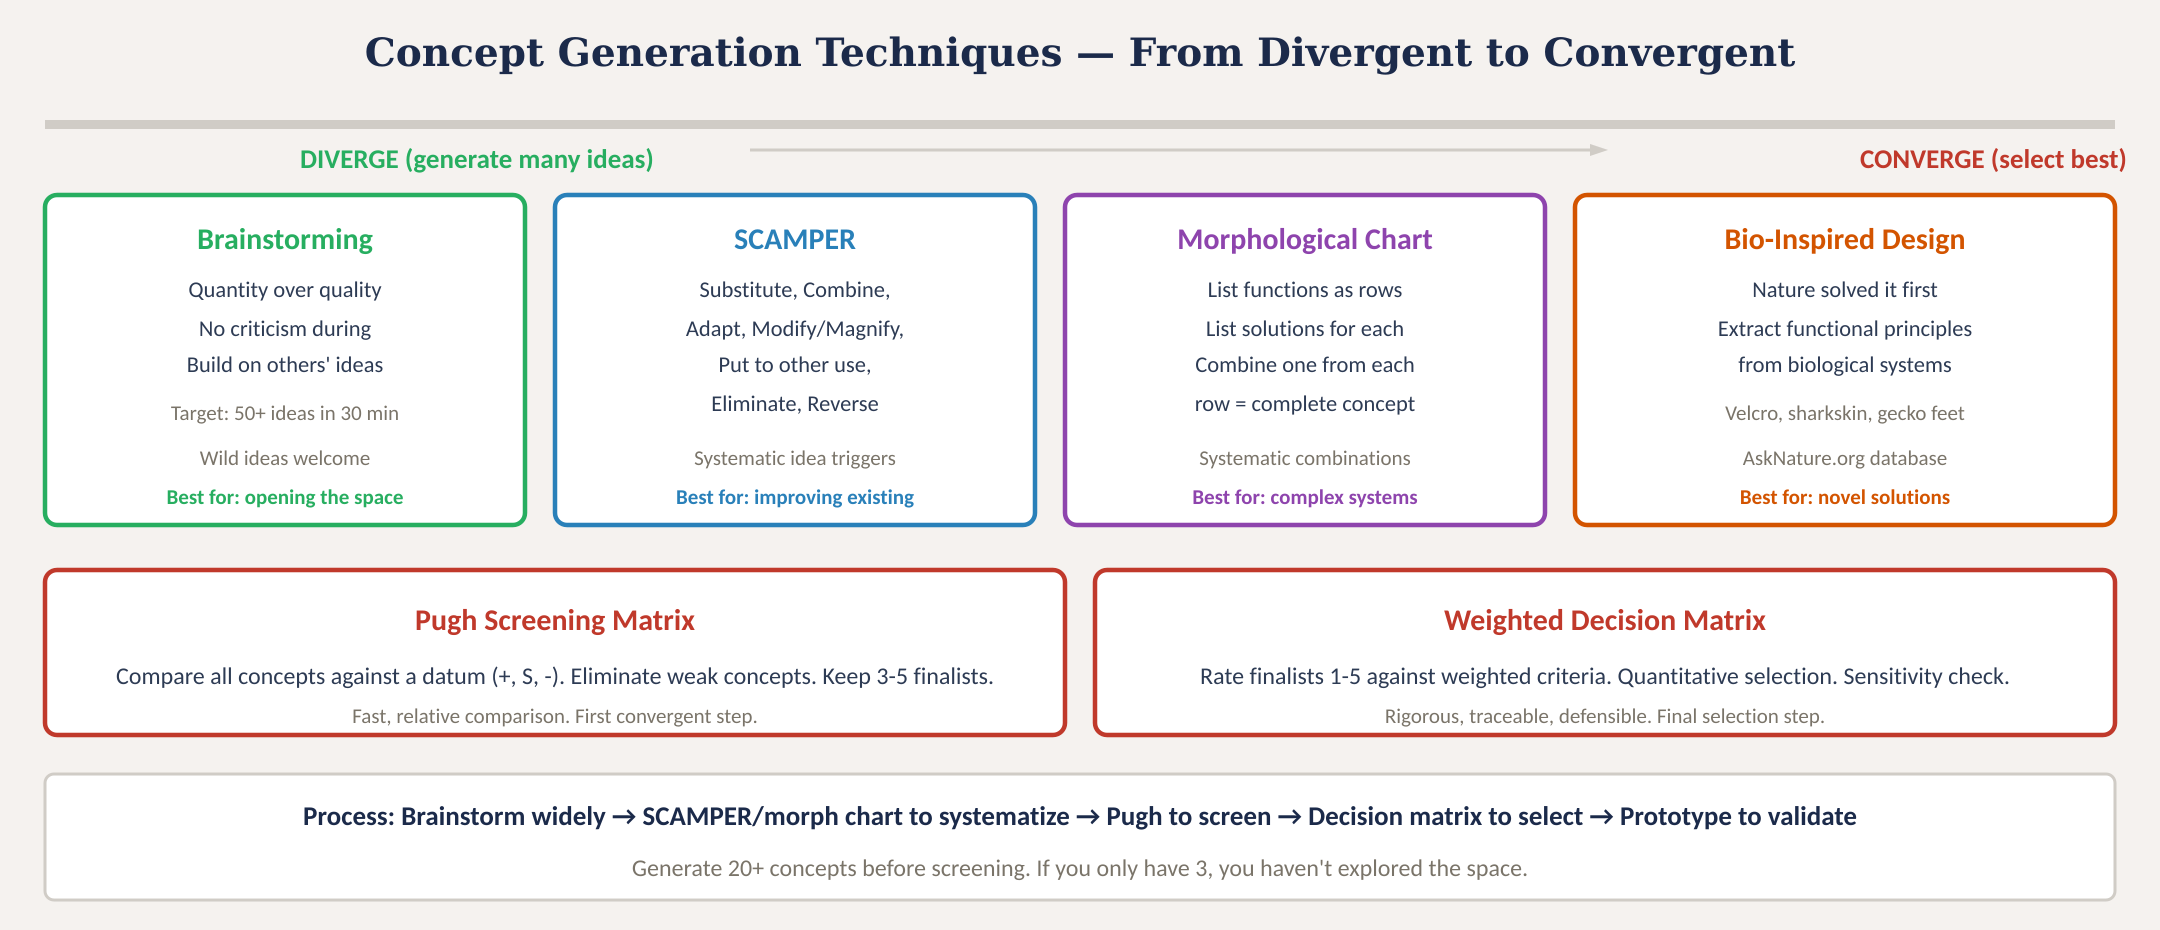
\includegraphics[width=\textwidth]{master_figs/fig_generation_techniques.png}
\caption{Concept generation techniques — divergent to convergent.}\end{figure}

\begin{figure}[htbp]\centering
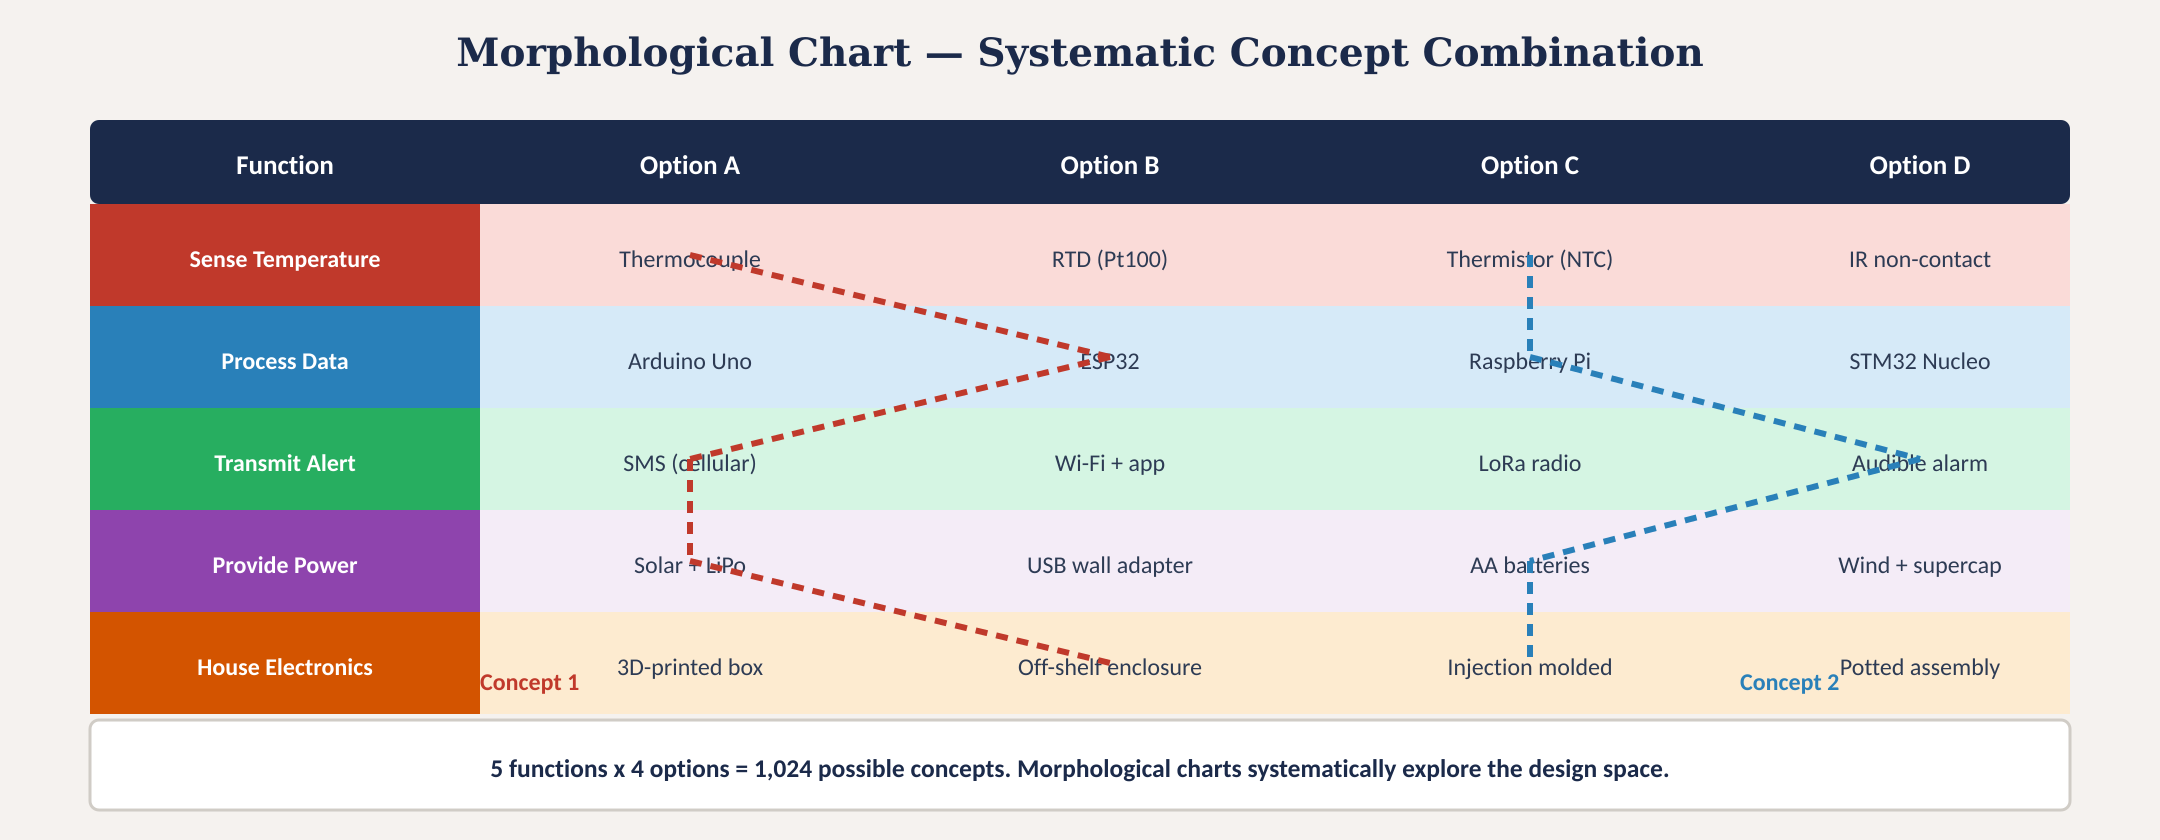
\includegraphics[width=\textwidth]{master_figs/fig_morphological_chart.png}
\caption{Morphological chart with systematic concept combinations.}\end{figure}

\begin{figure}[htbp]\centering
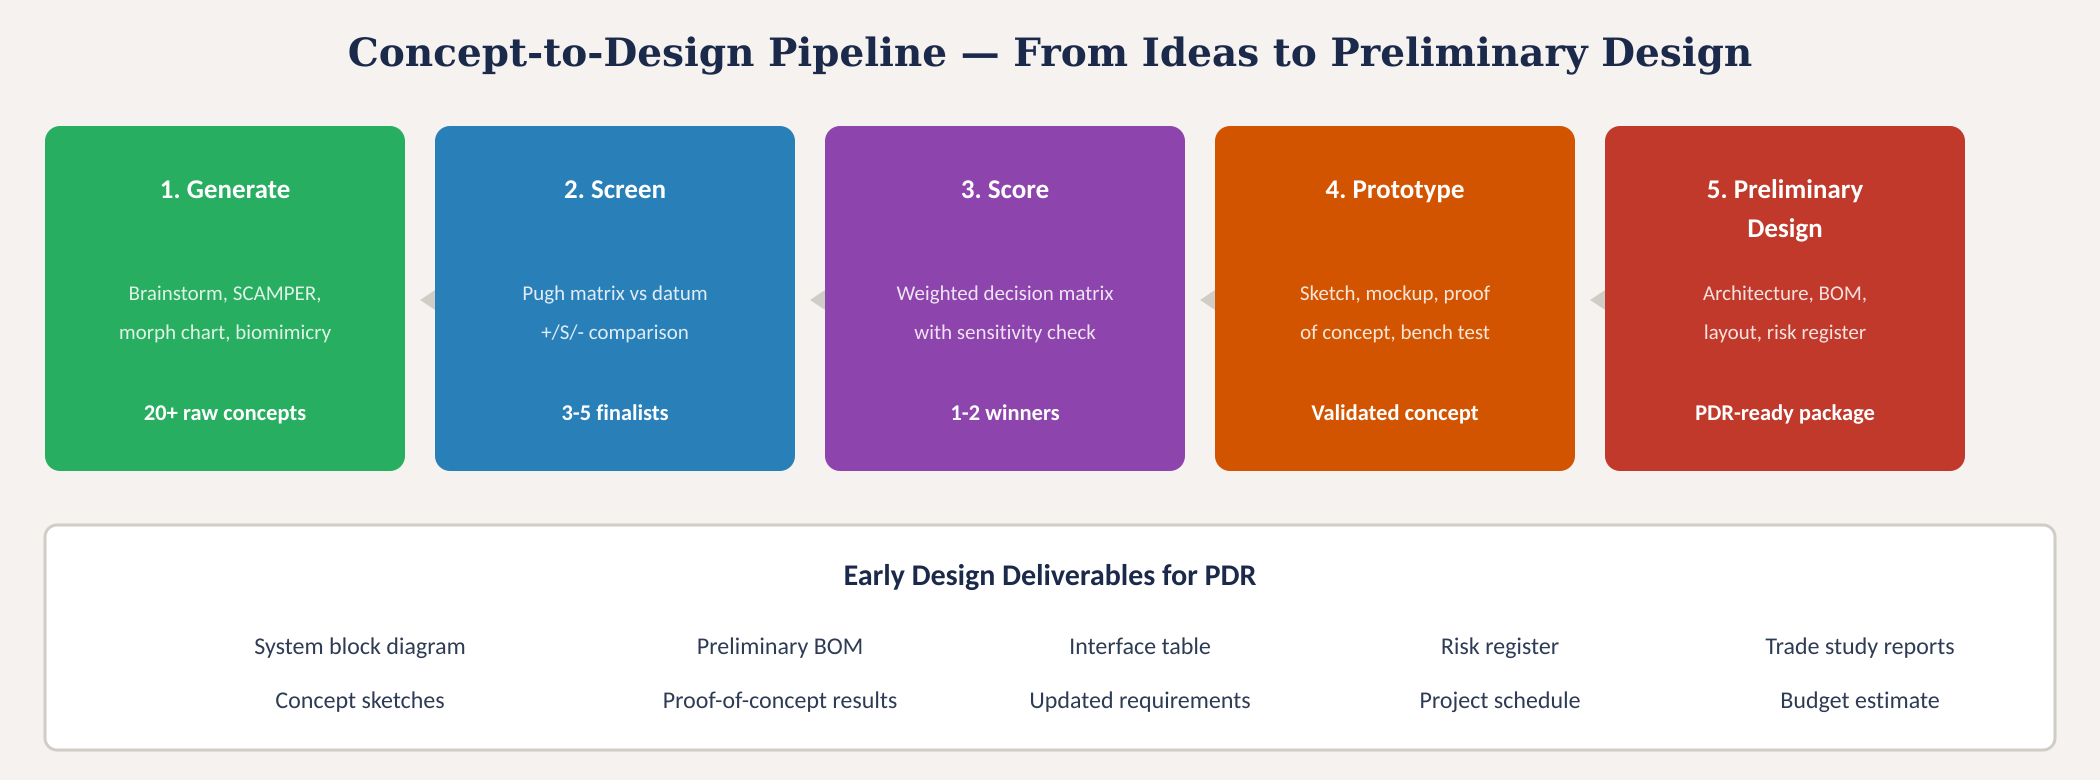
\includegraphics[width=\textwidth]{master_figs/fig_concept_pipeline.png}
\caption{Concept-to-design pipeline with PDR deliverables.}\end{figure}

\begin{figure}[htbp]\centering
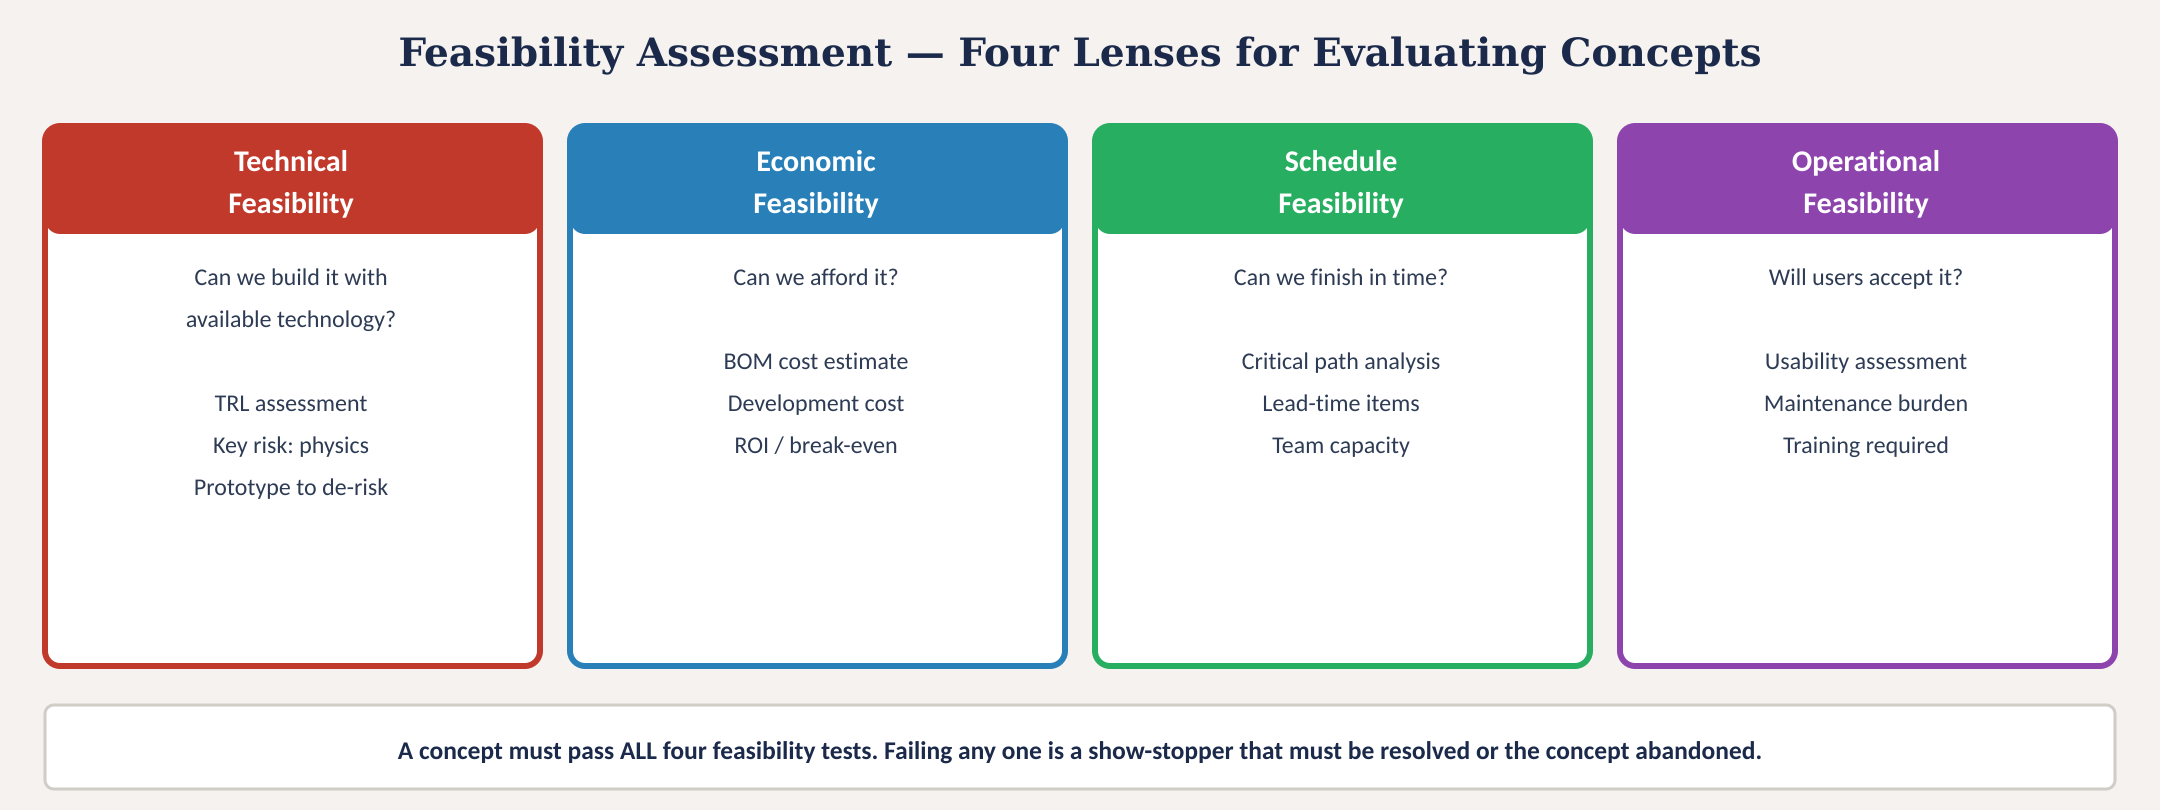
\includegraphics[width=\textwidth]{master_figs/fig_feasibility_assessment.png}
\caption{Four-lens feasibility assessment.}\end{figure}

\section{Reverse Engineering}
Reverse engineering is a structured process of disassembling an existing product to understand how it works. It builds engineering intuition and directly informs concept generation.

\subsection{The Reverse Engineering Process}
\begin{enumerate}[leftmargin=1.5em]
\item \textbf{Document the intact product}: photograph from all angles, measure overall dimensions, weigh it, record all labels and markings.
\item \textbf{Disassemble systematically}: remove fasteners in order, photograph each step, bag and label hardware. Use the right tools; forcing components causes damage that obscures design intent.
\item \textbf{Measure and catalog}: calipers for every component. Record materials (magnet test for ferrous metals, density test for plastics). Identify standard parts (bearings, fasteners, seals) by markings.
\item \textbf{Create the BOM}: part number, description, quantity, material, source, estimated cost.
\item \textbf{Create an exploded view}: CAD or carefully arranged photograph with callout labels.
\item \textbf{Functional analysis}: map each component to a function. Which are structural? Functional? Cosmetic? Note any clever design solutions.
\end{enumerate}

\subsection{What Reverse Engineering Reveals}
Assembly sequence (what goes in first must come out last. DFA insight). Material choices and why they were made. Manufacturing processes (injection molding witness lines, machining marks, weld joints). Standard vs.\ custom parts ratio. Design-for-cost decisions. Failure modes on used products (wear patterns).


\subsection{Reverse Engineering Outputs}
The analysis produces artifacts that feed directly into design:
\begin{itemize}[leftmargin=1.5em]
\item \textbf{Component inventory} with identified materials and manufacturing methods; informs DFM decisions (Injection Molding chapter).
\item \textbf{Interface inventory} of all accessible mounting points, electrical connections, and mechanical features; basis for ICDs (Chapter~2).
\item \textbf{Constraint list} documenting what your design cannot change; feeds requirements as non-functional constraints.
\item \textbf{Design insights} about proven approaches, failure modes, and opportunities; informs concept generation and FMEA.
\end{itemize}

\begin{tipbox}[Non-Destructive Constraint]
In MEGN~301, you must return the COTS product undamaged at the end of each class period. No drilling, cutting, gluing, or permanent modifications. Your add-on system must interface through existing features: existing screw holes, connectors, friction fits, clamps, or custom brackets. This mirrors real-world accessory development where your product must work with an existing platform without voiding its warranty.
\end{tipbox}

\subsection{From Reverse Engineering to Concept Generation}
The reverse engineering analysis directly feeds concept generation:
\begin{enumerate}[nosep,leftmargin=1.5em]
\item The interface inventory defines the physical envelope and connection options for your morphological chart.
\item The constraint list eliminates infeasible concepts before time is wasted developing them.
\item Design insights from the existing product provide proven approaches to build upon.
\item The component inventory reveals standard parts that you can reuse or specify.
\end{enumerate}


\section{Reverse Engineering}
Before generating new concepts, understand how existing solutions work. Reverse engineering builds engineering intuition and directly informs concept generation.

\subsection{The Reverse Engineering Process}
\begin{enumerate}[leftmargin=1.5em]
\item \textbf{Document the as-received state}: photograph from all angles before disassembly. Record weight, dimensions, labels, model numbers.
\item \textbf{Systematic disassembly}: remove fasteners in order, photograph each step, bag and label all hardware. Use the right tools; forcing components obscures design intent.
\item \textbf{Identify components and materials}: measure with calipers (not rulers). Magnet test for ferrous metals. Identify standard parts (bearings, fasteners, seals) by markings.
\item \textbf{Analyze the architecture}: create a block diagram showing subsystem connections. Identify functional groups, signal flows, and power distribution.
\item \textbf{Assess design decisions}: Why did the original designers make each choice? What manufacturing processes were used (injection molding witness lines, machining marks, weld joints)?
\item \textbf{Create deliverables}: BOM, exploded view photograph or CAD, functional analysis report.
\end{enumerate}

\subsection{What Reverse Engineering Reveals}
Assembly sequence (what goes in first comes out last; this drives DFA decisions). Material choices and manufacturing methods. Standard vs.\ custom parts ratio. Design-for-cost decisions. Wear patterns on used products that reveal failure modes.

\section{Generating Concepts}
\subsection{Diverge Then Converge}
The concept generation process has two distinct phases. \textbf{Divergent} thinking generates as many ideas as possible without evaluation — brainstorming, SCAMPER, morphological charts, and bio-inspired design. \textbf{Convergent} thinking systematically evaluates and selects — Pugh screening matrices and weighted decision matrices. Generate at least 20 concepts before screening any of them.

\subsection{Brainstorming Rules}
Defer judgment (no criticism during ideation). Go for quantity (target 50+ ideas in 30 minutes). Build on others' ideas (``yes, and...''). Encourage wild ideas (they contain seeds of insight). Sketch, don't just talk.

\subsection{SCAMPER}
Seven systematic triggers: Substitute, Combine, Adapt, Modify/Magnify, Put to other use, Eliminate, Reverse. Apply each to existing concepts or competitor products to generate variations.

\subsection{Morphological Charts}
List functions as rows (from functional decomposition), brainstorm 3--5 implementation options per function as columns. A complete concept = one option from each row. A 5$\times$4 chart produces 1,024 combinations — systematically exploring the design space.

\subsection{Bio-Inspired Design}
Extract functional principles from biological systems. Velcro from burdock burrs. Sharkskin for drag reduction. Use AskNature.org to search by function. TRIZ provides 40 inventive principles for resolving design contradictions.


\subsection{Stage 1: Pugh Screening Matrix}
Rate each concept against a datum (baseline concept) as better ($+$), same ($S$), or worse ($-$). No weights, no numbers; just qualitative comparison. Sum $+$'s and $-$'s. Eliminate concepts with many $-$'s. The survivors proceed to the weighted matrix.

\textbf{Rules}: at least 3 concepts plus the datum. Criteria from requirements only. If two concepts score similarly, do not eliminate either.

\subsection{Stage 2: Weighted Decision Matrix}
Rate surviving concepts 1--5 against weighted criteria (weights sum to 1.0). Calculate weighted score per option. Check sensitivity: vary each weight $\pm$0.05; if the winner changes, the selection is fragile.

\textbf{Common traps}: Straw-man alternatives (including clearly inferior options to make the favorite ``win''; every candidate must be legitimate). Anchoring on a favorite (assign ratings independently before group discussion). Criteria not from requirements (if a criterion does not trace to a requirement, remove it). Post-hoc weight adjustment (lock weights before scoring).

\textbf{Stage 1: Pugh Screening} — rate concepts as +/S/- against a datum. Fast, no weights. Eliminates clearly inferior options. \textbf{Stage 2: Weighted Decision Matrix} — rate finalists 1--5 against weighted criteria. Quantitative, traceable. Sensitivity check: if $\pm$0.05 weight change flips the winner, investigate further.


\section{Risk Assessment}
Risk management begins during concept selection, not after design. A \textbf{risk} is any event or condition that could prevent the system from meeting requirements. Every concept carries risks; the question is which are acceptable and which require mitigation.

\subsection{The Risk Matrix}
Risks are characterized by \textbf{likelihood} (1--5) and \textbf{consequence} (1--5). The product $L \times C$ gives the Risk Priority Number (RPN).

\begin{table}[htbp]\centering\small
\begin{tabularx}{\textwidth}{c X X}
\toprule
\textbf{Score} & \textbf{Likelihood} & \textbf{Consequence} \\
\midrule
1 & Very unlikely ($<$5\%) & Negligible (cosmetic, workaround exists) \\
2 & Unlikely (5--20\%) & Minor (schedule slip $<$1 week, minor rework) \\
3 & Possible (20--50\%) & Moderate (schedule slip 1--2 weeks, partial redesign) \\
4 & Likely (50--80\%) & Major (missed milestone, significant redesign) \\
5 & Almost certain ($>$80\%) & Catastrophic (project failure, safety hazard) \\
\bottomrule
\end{tabularx}
\caption{Risk likelihood and consequence scales.}
\end{table}

Action thresholds: RPN 1--4 = monitor, 5--9 = mitigate, 10--15 = mitigate aggressively, 16--25 = redesign or eliminate. Maintain a risk register from PDR through FDR, updating status at each review.

\subsection{Risk Mitigation Strategies}
Four options (in order of preference): \textbf{Avoid} (change the design to eliminate the risk), \textbf{Mitigate} (reduce likelihood or consequence), \textbf{Transfer} (shift risk to a vendor, insurer, or partner), \textbf{Accept} (document and monitor; only for low-RPN items).


\begin{greenshieldbox}[GreenShield: Risk Register at PDR]
\small
\begin{tabularx}{\textwidth}{X c c c X}
\toprule
\textbf{Risk} & \textbf{L} & \textbf{C} & \textbf{RPN} & \textbf{Mitigation} \\
\midrule
Solar panel insufficient in winter & 4 & 4 & 16 & Battery margin + Dec test \\
LoRa blocked by terrain & 3 & 3 & 9 & Site survey + repeater \\
Relay fails closed (heater on) & 2 & 5 & 10 & Thermal fuse backup \\
Thermocouple accuracy inadequate & 3 & 3 & 9 & In-situ calibration \\
MCU brown-out during Wi-Fi TX & 4 & 3 & 12 & 470\,$\mu$F decoupling \\
\bottomrule
\end{tabularx}
Red-zone: solar panel (16) and MCU brown-out (12) require active mitigation before CDR.
\end{greenshieldbox}

\section{Failure Modes and Effects Analysis (FMEA)}
FMEA systematically identifies potential failure modes, their effects, and their causes \emph{during design}; before hardware exists.

\subsection{Conducting a Design-Phase FMEA}
For each component or function:
\begin{enumerate}[nosep,leftmargin=1.5em]
\item List every way it can fail (\textbf{failure modes}).
\item Determine the effect of each failure on the system (\textbf{effects}).
\item Identify root causes.
\item Rate Severity (S), Occurrence (O), and Detection (D) on 1--10 scales.
\item Calculate RPN = S $\times$ O $\times$ D. Higher RPN = higher priority for corrective action.
\item Design corrective actions for the top-5 RPN items.
\end{enumerate}

\begin{table}[htbp]\centering\small
\begin{tabularx}{\textwidth}{l l X c c c c}
\toprule
\textbf{Component} & \textbf{Failure Mode} & \textbf{Effect} & \textbf{S} & \textbf{O} & \textbf{D} & \textbf{RPN} \\
\midrule
Temp sensor & Reads high & Heater never activates; crop loss & 8 & 3 & 4 & 96 \\
Relay & Stuck closed & Heater runs continuously; fire risk & 9 & 2 & 6 & 108 \\
MCU & Brown-out reset & System offline during freeze event & 7 & 4 & 5 & 140 \\
GSM module & No signal & Alert not sent; operator unaware & 5 & 3 & 3 & 45 \\
Power supply & Fails open & Complete system loss & 8 & 2 & 7 & 112 \\
\bottomrule
\end{tabularx}
\caption{Example design-phase FMEA for GreenShield frost protection system.}
\end{table}

The MCU brown-out (RPN 140) is the highest-priority item; address it with decoupling capacitors, a voltage supervisor, and separate power routing (see Chapter~9).


\subsection{Prototype Types in Detail}
\textbf{Proof of Concept (PoC)}: validates the riskiest technical assumption. Build the minimum hardware/software to answer one question: ``Does the physics/algorithm/mechanism work?'' Example: a breadboard circuit with just the sensor and MCU to verify temperature accuracy before designing the full system. Build time: 1--3 days. Quality: ugly is fine.

\textbf{Form/Fit prototype}: verifies physical compatibility. 3D-print the enclosure, mount real components, check cable routing and assembly sequence. No electronics need to function; this is a geometry check. Build time: 2--4 days. \textbf{Always print at 1:1 scale and test-fit real components.}

\textbf{Looks-Like/Works-Like}: a near-complete system that demonstrates both form and function. This is your CDR deliverable. It should be close to the final design but may use breadboard wiring or temporary mounting. Build time: 1--3 weeks.

\textbf{Minimum Viable Product (MVP)}: the simplest version that delivers value to the stakeholder. It meets the MUST requirements but may defer SHOULD and COULD features. The MVP is what you demonstrate at FDR.

\begin{tipbox}[Build the Highest-Risk PoC First]
Identify the single technical element most likely to fail. Build a PoC for that element before anything else. If it fails, you learn early and can pivot. If it works, confidence increases and the rest of the design proceeds on solid ground.
\end{tipbox}

\section{Prototyping and Feasibility}
Four prototype types: Proof of Concept (does the physics work?), Form/Fit (does it fit the space?), Looks-Like/Works-Like (can the team build the full system?), and Minimum Viable Product (does the stakeholder accept it?). Build the PoC for the highest-risk element FIRST.

\subsection{Feasibility Assessment}
Every concept must pass four tests: \textbf{Technical} (can we build it?), \textbf{Economic} (can we afford it?), \textbf{Schedule} (can we finish in time?), \textbf{Operational} (will users accept it?). Failing any one is a show-stopper.


\section{Design Documentation}
Complete design documentation enables someone else to build, test, and maintain your system without your presence.

\subsection{Bill of Materials (BOM)}
Required columns: item number, part number, description, quantity, material, vendor, vendor part number, unit cost, lead time, status (ordered/received/installed). Organize hierarchically: Level~0 = system, Level~1 = subsystems, Level~2 = assemblies, Level~3 = parts. \textbf{Every part must appear in the BOM.}

\subsection{Wiring Diagrams and Schematics}
\textbf{Schematics} show electrical connections using standard symbols; the ``source code'' of hardware. \textbf{Wiring diagrams} show physical routing with connector pin assignments and wire colors/gauges. Both are required: schematics for design intent, wiring diagrams for assembly.

\subsection{Software Architecture and Flowcharts}
Document firmware with: (1) state-machine diagram showing all states and transitions, (2) data flow diagram (sensor $\to$ processing $\to$ actuator), (3) pin mapping table (GPIO $\to$ function $\to$ component), (4) communication protocol definitions (message formats, baud rates, addresses).

\subsection{CAD Models and Engineering Drawings}
CAD models define geometry. Engineering drawings communicate that geometry with dimensions, tolerances, surface finishes, and notes. Every custom part requires a drawing. Standard parts reference vendor part numbers; no drawing needed.

\begin{tipbox}[Plan B Components]
For every critical component, identify a Plan~B; an alternative from a different vendor meeting the same requirements. Lead times slip, parts go out of stock, and vendors make mistakes. A Plan~B list saves weeks of panic.
\end{tipbox}

\begin{tipbox}[Free Electronics Supplies]
Before ordering, check the MEGN~301 electronics inventory in the ME shop. Common components (resistors, capacitors, LEDs, wire, headers, breadboards) are available at no cost. Check the shared inventory spreadsheet first.
\end{tipbox}

\begin{tipbox}[The Spring Break Shipping Trap]
Orders placed the week before spring break often arrive \emph{during} break when no one is on campus. Plan so critical parts arrive at least one week before any closure. International suppliers (AliExpress, LCSC): allow 3--4 weeks. McMaster-Carr ships next-day to Golden.
\end{tipbox}

\begin{greenshieldbox}[GreenShield: Morphological Chart]
\small
\begin{tabularx}{\textwidth}{l X X X}
\toprule
\textbf{Function} & \textbf{Option A} & \textbf{Option B} & \textbf{Option C} \\
\midrule
Sense Temp & DS18B20 digital & BME280 (T/H/P) & Thermocouple + amp \\
Control Logic & ESP32 (Wi-Fi) & Arduino Nano & RPi Zero \\
Heat Actuator & Ceramic heater + relay & Heat lamp + relay & Heated water loop \\
Communication & SMS via SIM800L & Wi-Fi + cloud & LoRa to base station \\
Power Source & 120 VAC wall adapter & 12V solar + battery & PoE \\
\bottomrule
\end{tabularx}

\textbf{Concept 1 (Grid-Connected)}: DS18B20 + ESP32 + Ceramic heater + Wi-Fi + Wall adapter. Lowest cost, simplest, requires AC power.

\textbf{Concept 2 (Off-Grid Solar)}: BME280 + ESP32 + Ceramic heater + LoRa + Solar+battery. Grid-independent, higher cost, battery sizing critical.

\textbf{Concept 3 (Industrial)}: Thermocouple + RPi + Heated water loop + SMS + PoE. Highest capability and cost.
\end{greenshieldbox}

\begin{greenshieldbox}[GreenShield: Risk Assessment for Concept 2 (Off-Grid)]
\textbf{Technical risks}: (1) Solar panel sizing for Colorado winters, December insolation is 3.5 peak sun hours vs.\ 6.5 in July. Battery must sustain 3 consecutive cloudy days. (2) LoRa range through polycarbonate glazing, 3--6\,dB attenuation at 915\,MHz.

\textbf{Schedule risk}: Solar charge controller + BMS integration adds 2 weeks. If the team is behind at CDR, this is a schedule-buster.

\textbf{Economic risk}: Solar (\$25) + charge controller (\$15) + LiPo (\$20) + LoRa (\$12 ea) = \$84 for power/comms vs.\ \$8 for Concept 1.

\textbf{Verdict}: High-risk for 16-week schedule. Recommend Concept 1 with upgrade path.
\end{greenshieldbox}

\begin{keyconceptbox}[Industry SE Parallels]
\begin{itemize}[nosep,leftmargin=1.5em]
\item \textbf{INCOSE SEH 4th ed.}: Sec.\ 4.3 (Architecture Definition), Sec.\ 4.4 (Design Definition).
\item \textbf{NASA SP-2016-6105 Rev 2}: Ch.\ 4.4 (Design Solution Definition), Ch.\ 6.6 (Decision Analysis).
\item \textbf{IEEE 1220}: Standard for systems engineering process management.
\end{itemize}
\end{keyconceptbox}

\section{Artifact Handoff: What Chapter 3 Produces}
\begin{table}[htbp]\centering\small
\begin{tabularx}{\textwidth}{l X l}
\toprule
\textbf{Artifact} & \textbf{Description} & \textbf{Forward Reference} \\
\midrule
Morphological Chart & Functions $\times$ implementation options & PDR documentation \\
Trade Study / Decision Matrix & Weighted evaluation of top concepts & PDR deliverable \\
Selected Concept Package & Block diagram, preliminary BOM, risk assessment & Ch.~4, CDR \\
Design Documentation & BOM, schematics, CAD, software architecture & Ch.~5 (integration), FDR \\
\bottomrule
\end{tabularx}
\end{table}

\section{Structured Creativity Methods}
\subsection{Morphological Analysis}
Morphological analysis systematically generates concepts by combining solutions for each function:

(1) List the key functions the product must perform (sense, actuate, power, communicate, enclose).

(2) For each function, brainstorm 3--5 alternative solutions (for ``sense temperature'': thermocouple, RTD, thermistor, IR sensor, bimetallic strip).

(3) Arrange in a matrix with functions as rows and solutions as columns.

(4) Generate concepts by selecting one solution from each row and combining them. A 5-function matrix with 4 alternatives per function yields $4^5 = 1024$ theoretical combinations.

(5) Screen the combinations for compatibility (not all combinations are physically or economically feasible) and select the 5--10 most promising for detailed evaluation.

\subsection{SCAMPER Method}
A checklist for modifying existing designs: \textbf{S}ubstitute (different material, component, process), \textbf{C}ombine (merge two functions into one component), \textbf{A}dapt (borrow a solution from another domain), \textbf{M}odify (change size, shape, color, texture), \textbf{P}ut to other use (use the product for a different application), \textbf{E}liminate (remove a feature or component), \textbf{R}everse/Rearrange (change the order, orientation, or hierarchy).

\subsection{Biomimicry}
Nature has solved many engineering problems through evolution. Look to biological systems for inspiration: gecko feet for adhesion without glue, termite mounds for passive ventilation, shark skin for drag reduction, pinecones for humidity-responsive actuation, and bone structures for lightweight strength. In MEGN~301, biomimicry is particularly relevant for thermal management (how do desert animals stay cool?), fluid handling (how do trees pump water 100\,m upward?), and structural design (how do shells achieve high strength-to-weight ratios?).

\section{Concept Selection: Beyond the Pugh Matrix}
\subsection{Weighted Decision Matrix}
An enhanced Pugh matrix where criteria are weighted by importance:

(1) Define 6--10 evaluation criteria (performance, cost, complexity, reliability, manufacturability, safety, sustainability).

(2) Assign weights (total $= 100\%$). Typically: performance 25\%, cost 20\%, manufacturability 15\%, reliability 15\%, safety 10\%, sustainability 10\%, aesthetics 5\%.

(3) Score each concept against each criterion on a 1--5 scale.

(4) Compute weighted scores and rank.

(5) Perform sensitivity analysis: vary the weights by $\pm$20\% and check whether the ranking changes. If it does, the decision is sensitive to subjective weighting and requires careful justification.

\subsection{Concept Testing}
Before committing to a concept, build a quick proof-of-concept prototype to validate the highest-risk element. This is \emph{not} the final prototype; it is a focused experiment to answer one question: ``does this approach actually work?''

For a thermal control system: the highest risk might be ``can we maintain $\pm$1\,\degC{} with a 200\,W heater and PID control?'' Build a minimal system (heater, thermocouple, Arduino, relay) and test. The result either validates the concept (proceed) or invalidates it (pivot), saving weeks of detailed design effort.

\section{Design for the GreenShield Competition}
The GreenShield project evaluation criteria guide concept selection:

\textbf{Innovation (25\%)}: novel application of engineering principles, creative use of materials or processes, unique approach to the problem.

\textbf{Technical execution (30\%)}: quality of the requirements, design, fabrication, and testing. Meets all specified requirements.

\textbf{Sustainability (20\%)}: environmental impact assessment, design for disassembly, material selection, energy efficiency.

\textbf{Communication (15\%)}: quality of documentation, presentations, and demonstrations.

\textbf{Teamwork (10\%)}: evidence of effective collaboration, equitable contribution, and conflict resolution.

Concepts should be selected not only for technical merit but for alignment with these evaluation criteria. A technically simple but highly sustainable and well-documented project may score higher than a technically ambitious project that fails to meet half its requirements.
\section{Failure Modes and Effects Analysis (FMEA) During Design}
FMEA is not a post-mortem performed after the system fails. It is a \textbf{design tool} that prevents failures by forcing the team to systematically ask ``what can go wrong?'' during the concept and early design phase, when changes are cheap.

\subsection{When to Perform FMEA}
Perform FMEA \emph{before} CDR, ideally during concept selection (this chapter) or architecture definition (Chapter~3). Waiting until Operations \& Maintenance (Chapter~7) transforms FMEA from a prevention tool into an autopsy. The cost of discovering a failure mode scales exponentially with project phase: \$1 at concept, \$10 at CDR, \$100 at integration, \$1000 at FDR.

\subsection{The FMEA Process}
For each component or function in the design:

(1) \textbf{Failure mode}: how can it fail? Be specific. ``Motor fails'' is too vague. ``Motor stalls due to overcurrent'' or ``motor shaft coupling slips under load'' are actionable.

(2) \textbf{Effect}: what happens to the system if this failure occurs? ``System overheats because heater stays ON'' or ``pump stops, fluid stagnates.''

(3) \textbf{Cause}: what could trigger this failure? ``Insufficient motor torque for the load'' or ``set screw loosened by vibration.''

(4) \textbf{Severity (S)}: how bad is the effect? 1 (negligible) to 10 (safety hazard, injury possible).

(5) \textbf{Occurrence (O)}: how likely is the cause? 1 (extremely unlikely) to 10 (almost certain).

(6) \textbf{Detection (D)}: how likely is the failure to be detected \emph{before} it causes harm? 1 (certain detection) to 10 (no detection mechanism).

(7) \textbf{Risk Priority Number}: $\text{RPN} = S \times O \times D$. Maximum RPN $= 1000$. Prioritize mitigation actions for the highest RPNs.

\subsection{FMEA for GreenShield Projects}
At minimum, analyze the top 10 failure modes covering: power system failures (short circuit, reverse polarity, battery overdischarge), sensor failures (open circuit, drift, saturation), actuator failures (stall, runaway, mechanical failure), communication failures (WiFi dropout, I2C bus hang), and software failures (watchdog timeout, state machine deadlock).

\begin{greenshieldbox}[GreenShield: FMEA Template]
\begin{tabularx}{\textwidth}{p{2cm} p{2cm} p{2cm} c c c c}
\toprule
\textbf{Component} & \textbf{Failure Mode} & \textbf{Effect} & \textbf{S} & \textbf{O} & \textbf{D} & \textbf{RPN} \\
\midrule
Heater SSR & Fails ON (shorted) & Uncontrolled heating, fire risk & 9 & 2 & 4 & 72 \\
ESP32 & Firmware crash & All outputs freeze at last state & 7 & 4 & 3 & 84 \\
LiPo battery & Over-discharge & Battery damage, swelling & 8 & 3 & 2 & 48 \\
Motor coupling & Set screw loosens & Motor spins but load doesn't move & 4 & 5 & 6 & 120 \\
Thermocouple & Wire breaks (open) & Reading jumps to max or NaN & 6 & 3 & 2 & 36 \\
\bottomrule
\end{tabularx}
\vspace{0.3em}
The motor coupling (RPN $= 120$) is the highest priority. Mitigation: use Loctite 242 on the set screw and add a flat on the shaft. The ESP32 crash (RPN $= 84$) is second: mitigation is the hardware watchdog timer and fail-safe relay (Chapter~15 in the 300 notes, Chapter~12 in this document).
\end{greenshieldbox}
\section{Practice Questions}
\begin{enumerate}[leftmargin=1.5em]
\item Create a morphological chart for a campus recycling station with at least 4 functions and 3 options each. Trace two complete concept paths.
\item Your team brainstormed only 5 concepts in 20 minutes. What went wrong? What facilitation techniques would you use to increase output?
\item A trade study produces scores of 3.82 vs 3.79 between two motor options. What do you do?
\item Your proof-of-concept test shows the sensor accuracy is 1.2$^{\circ}$ C against a 0.5$^{\circ}$ C requirement. What are your options?
\item You are reverse-engineering a consumer drone. During disassembly you find a small metal weight glued inside one motor arm. What is its likely purpose, and what does this tell you about the manufacturer's design process?
\item Your team's BOM lists ``motor'' with no part number, no vendor, and no specifications. Why is this a problem, and what minimum information must every BOM entry contain?
\end{enumerate}

\subsection{Answers}
\begin{enumerate}[leftmargin=1.5em]
\item Example morphological chart for campus recycling station:

\small
\begin{tabularx}{\textwidth}{l X X X}
\toprule
Function & Option A & Option B & Option C \\
\midrule
Identify material & RFID tag & Camera + ML & Weight sensor \\
Sort mechanism & Rotating drum & Conveyor + diverter & Gravity chute \\
User interface & Touchscreen & Button panel & Voice commands \\
Compaction & Hydraulic press & Screw auger & Gravity (none) \\
\bottomrule
\end{tabularx}
\normalsize

\textbf{Concept 1}: RFID + Conveyor + Touchscreen + Hydraulic = high accuracy, high cost, complex.

\textbf{Concept 2}: Camera + Gravity chute + Button + None = moderate accuracy, low cost, simple.

\item Too few concepts: (a) Criticism crept into brainstorming (evaluation during ideation kills creativity). (b) Team anchored on a favorite concept. (c) No systematic technique used. Fixes: enforce ``no criticism'' rule with a timer, use SCAMPER to force variations, require sketches not just words, set a minimum of 20 ideas before stopping.

\item A 0.03 margin is within noise. Sensitivity analysis: vary each weight by $\pm$0.05. If the winner changes, the selection is not robust. Options: prototype both finalists, gather better data on the most differentiating criterion, or choose based on a secondary factor (availability, team familiarity).

\item Options: (a) Improve the sensor (better calibration, thermal isolation, averaging algorithm). (b) Change the sensor (switch to RTD from thermocouple, higher accuracy, higher cost). (c) Relax the requirement (stakeholder may accept $\pm$1.0\,\degC{}, verify with stakeholder before changing). (d) Add a correction factor (calibrate against a reference and apply polynomial correction in firmware). Always investigate the requirement validity before redesigning hardware.

\item The weight is likely for vibration balancing. The motor arm, with motors and propellers, has a center of gravity that is not perfectly symmetric. The manufacturer added a counterweight to tune the balance and reduce vibration. This tells you the manufacturer performs dynamic balancing as a post-assembly step; a quality control measure that indicates vibration was a problem in earlier designs.

\item ``Motor'' without specifications is useless for procurement, testing, or replacement. A vendor cannot fill this order. Minimum BOM entry: manufacturer (e.g., Pololu), part number (e.g., 4843), description (``12V 100RPM DC gearmotor''), key specs (voltage, no-load speed, stall torque, rated current), quantity, unit cost, vendor, and lead time.
\end{enumerate}


\chapter{Verification, Validation \& Test Plans}

\vspace{1em}


\vspace{1em}

\section{Verification vs.\ Validation}
\begin{figure}[htbp]\centering
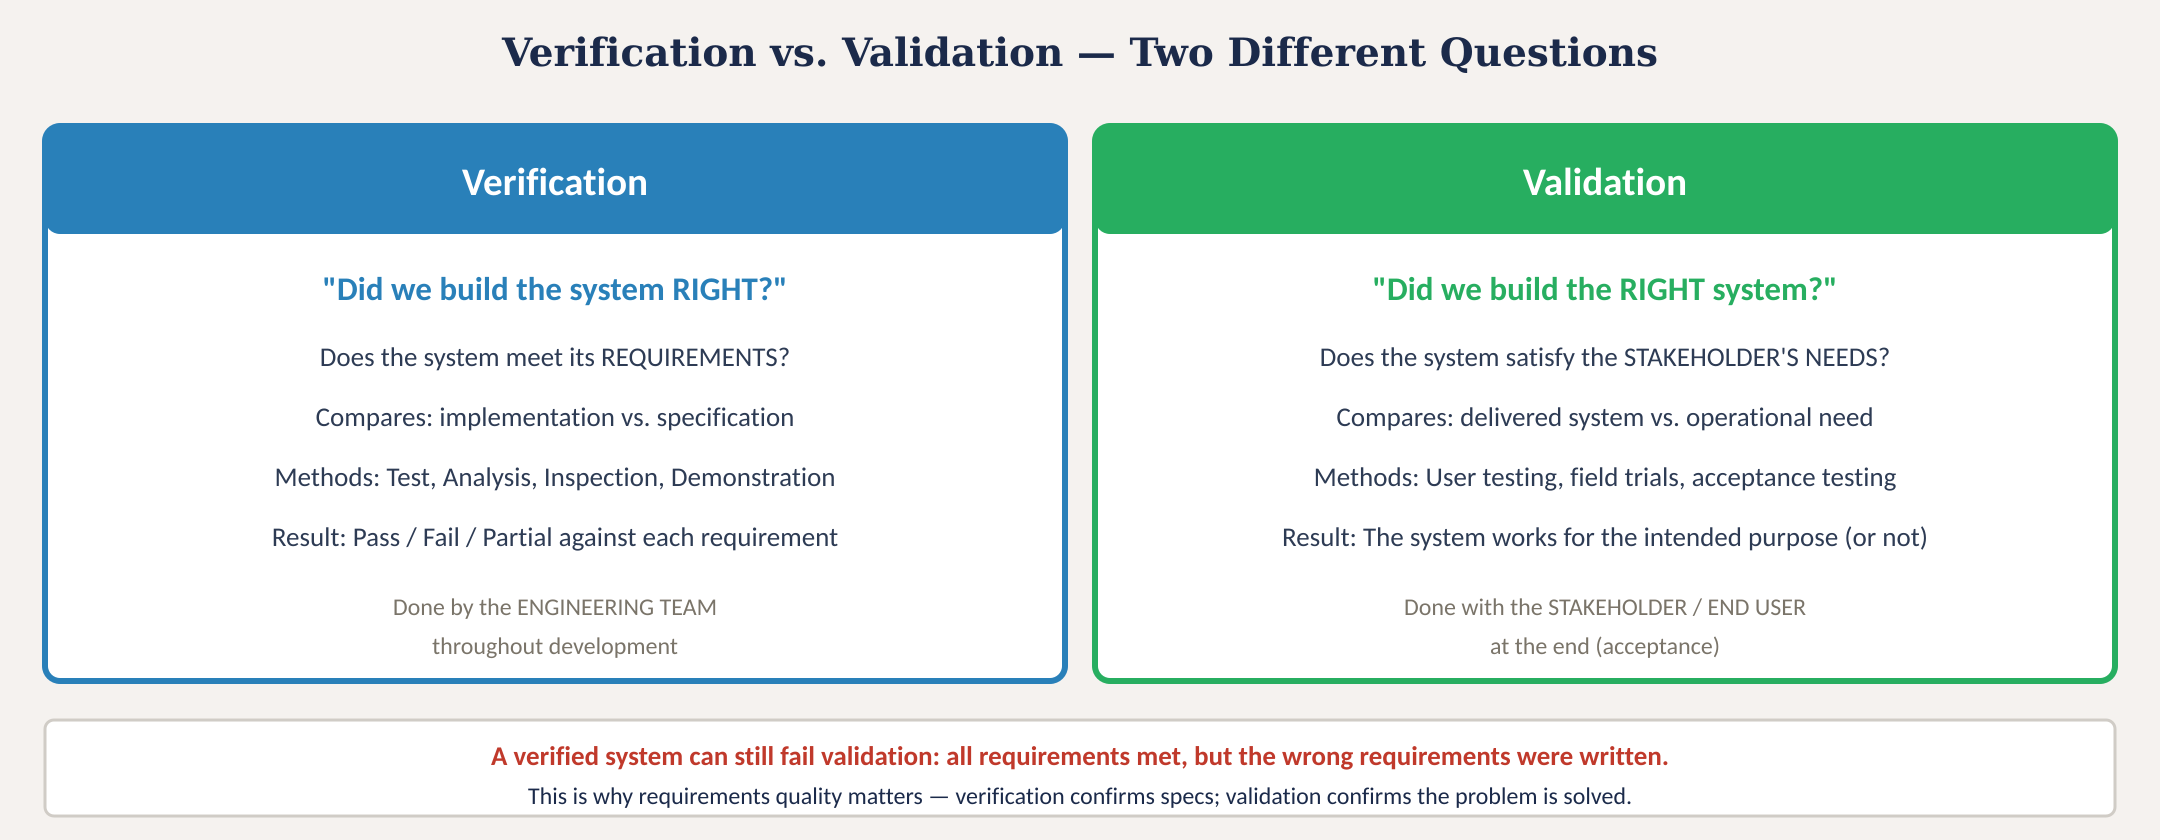
\includegraphics[width=\textwidth]{master_figs/fig_vv_comparison.png}
\caption{Verification (meets requirements) vs.\ validation (meets needs); two different questions.}\label{fig:vv}
\end{figure}

\textbf{Verification} asks: ``Did we build the system RIGHT?'' It compares the implemented system against the written specification. Done by the engineering team using Test, Analysis, Inspection, or Demonstration (TAID). Each requirement receives an individual PASS/FAIL verdict.

\textbf{Validation} asks: ``Did we build the RIGHT system?'' It compares the delivered system against the stakeholder's actual operational need. Done with the stakeholder through user testing, field trials, or acceptance testing.

\begin{warningbox}[A Verified System Can Fail Validation]
All requirements met perfectly, but the wrong requirements were written. This is why requirements quality matters; verification confirms specs; validation confirms the problem is actually solved. You need both.
\end{warningbox}

\section{Four Verification Methods: TAID}
\begin{figure}[htbp]\centering
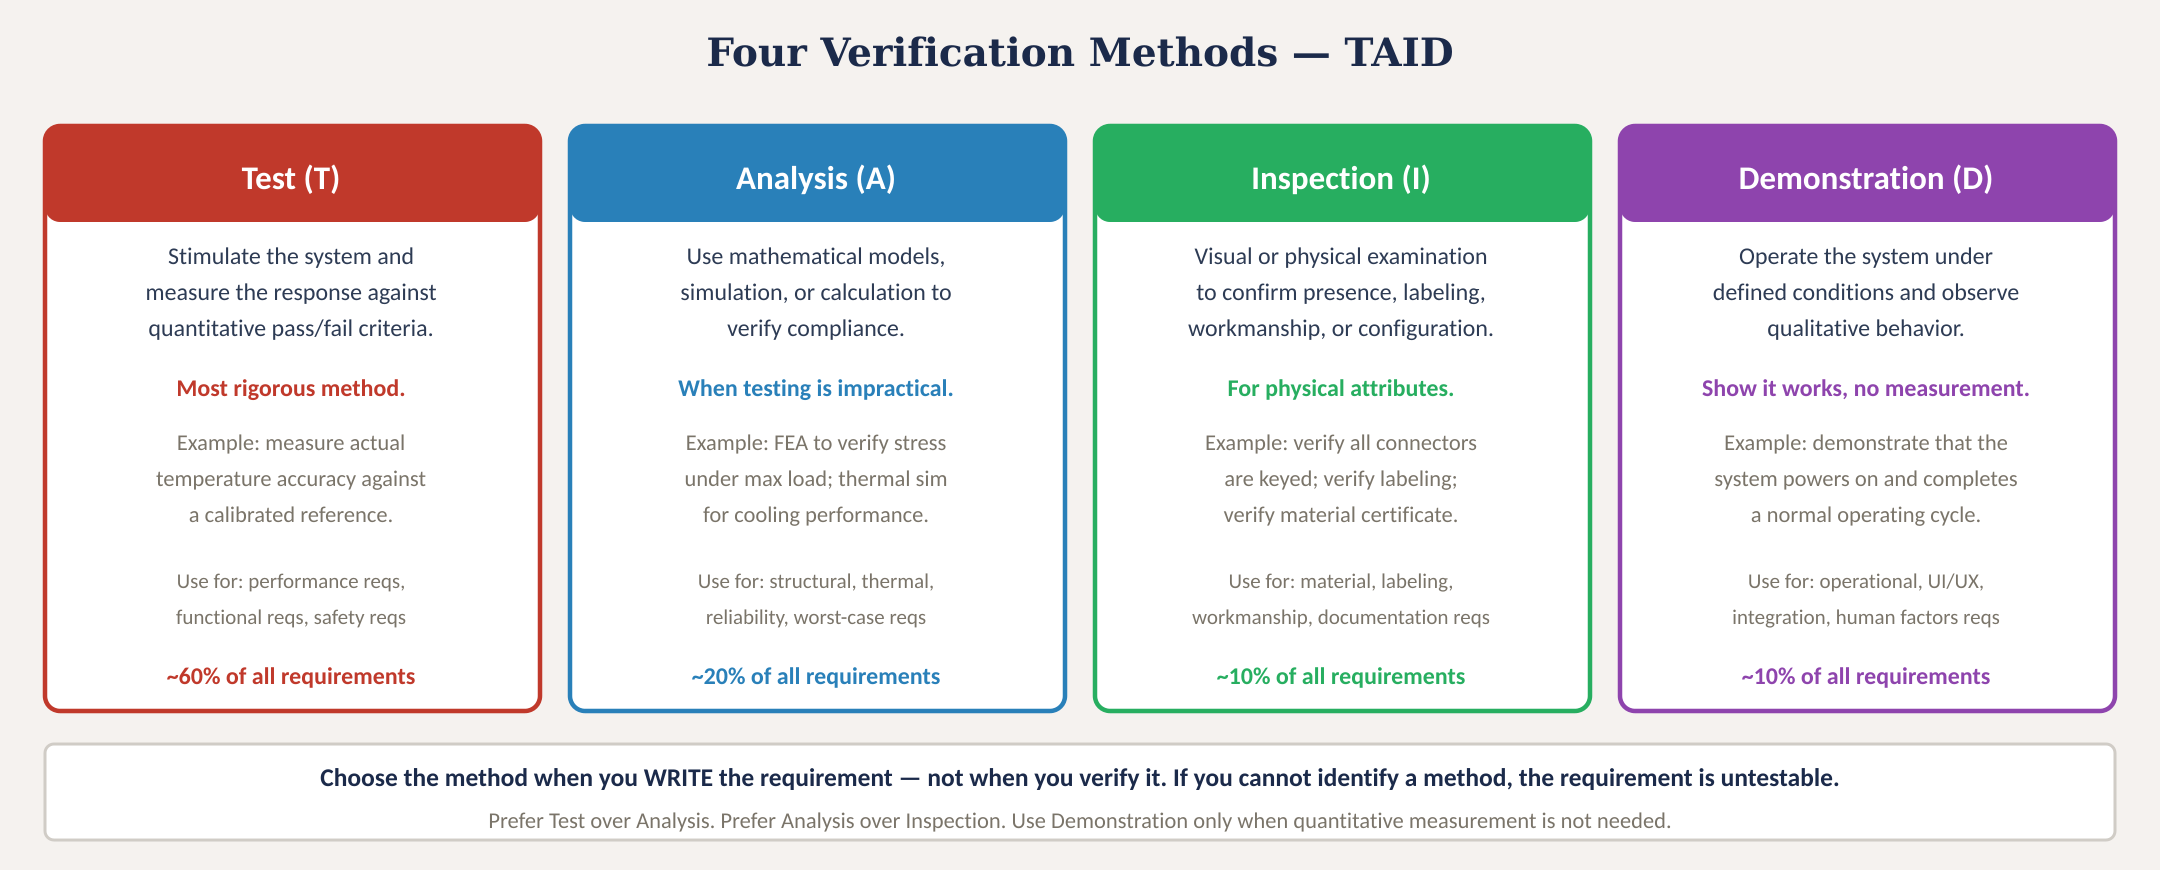
\includegraphics[width=\textwidth]{master_figs/fig_taid_methods.png}
\caption{Test, Analysis, Inspection, and Demonstration with usage percentages and selection guidance.}\label{fig:taid}
\end{figure}

\begin{itemize}[leftmargin=1.5em]
\item \textbf{Test (T, $\$\sim\$$60\% of reqs)}: Stimulate the system and measure the response against quantitative criteria. Most rigorous. Preferred whenever feasible.
\item \textbf{Analysis (A, $\$\sim\$$20\%)}: Mathematical models, simulation, or calculation. Used when testing is impractical (FEA, thermal sim, worst-case analysis). Must document assumptions.
\item \textbf{Inspection (I, $\$\sim\$$10\%)}: Visual/physical examination; presence, labeling, workmanship, material certificates.
\item \textbf{Demonstration (D, $\$\sim\$$10\%)}: Operate under defined conditions and observe qualitative behavior. No measurement. Used when quantitative testing is not needed.
\end{itemize}

\begin{tipbox}[Assign the Method When You Write the Requirement]
If you cannot identify a verification method, the requirement is untestable and must be rewritten. The method check is the single best quality gate for requirements.
\end{tipbox}

\section{Writing Test Plans}
\subsection{What Makes a Good Test Plan}
The gold standard: another engineer with no project knowledge can reproduce your results exactly. Five qualities: \textbf{Traceable} (maps to requirement IDs), \textbf{Reproducible} (specific enough for independent replication), \textbf{Binary} (quantitative pass/fail, no judgment calls), \textbf{Complete} (all sections filled), \textbf{Executed as written} (no ad-hoc deviations).

\subsection{Test Procedure Structure}
\begin{figure}[htbp]\centering
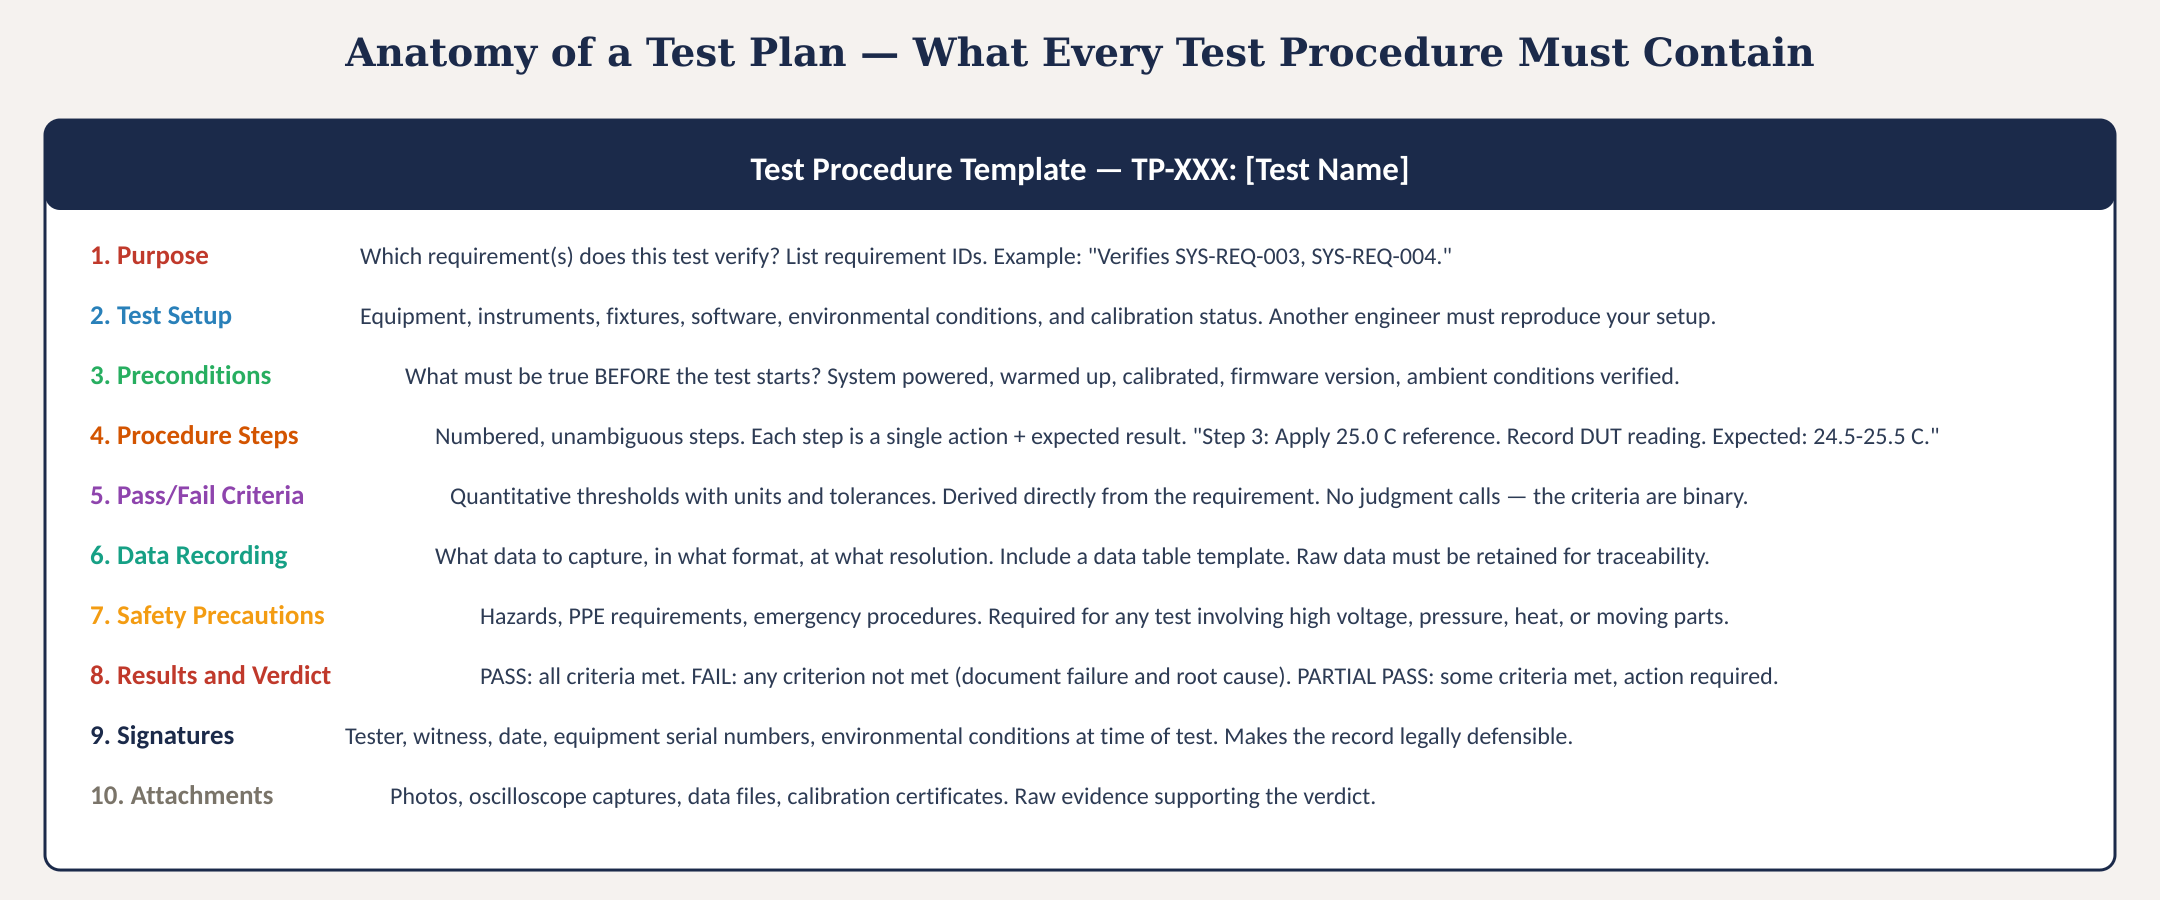
\includegraphics[width=\textwidth]{master_figs/fig_test_plan_template.png}
\caption{Complete test procedure template with all 10 required sections.}\label{fig:tp}
\end{figure}

Every test procedure contains: (1) Purpose; requirement IDs verified; (2) Test setup; equipment with model numbers and calibration; (3) Preconditions; system state before starting; (4) Procedure steps; numbered, single-action, imperative voice, with expected results; (5) Pass/fail criteria; quantitative thresholds from requirements; (6) Data recording; format, resolution, blank table; (7) Safety precautions; (8) Results and verdict; (9) Signatures; (10) Attachments.

\subsection{Writing Good Procedure Steps}
Each step is a single action with an expected result. Use specific values (``Set reference bath to 25.0 $\pm$ 0.1\,$^{\circ}$ C''), not vague instructions (``check temperature''). Include wait times for stabilization. Imperative voice: ``Set\ldots'' ``Record\ldots'' ``Verify\ldots''

\section{Handling Results}
\begin{figure}[htbp]\centering
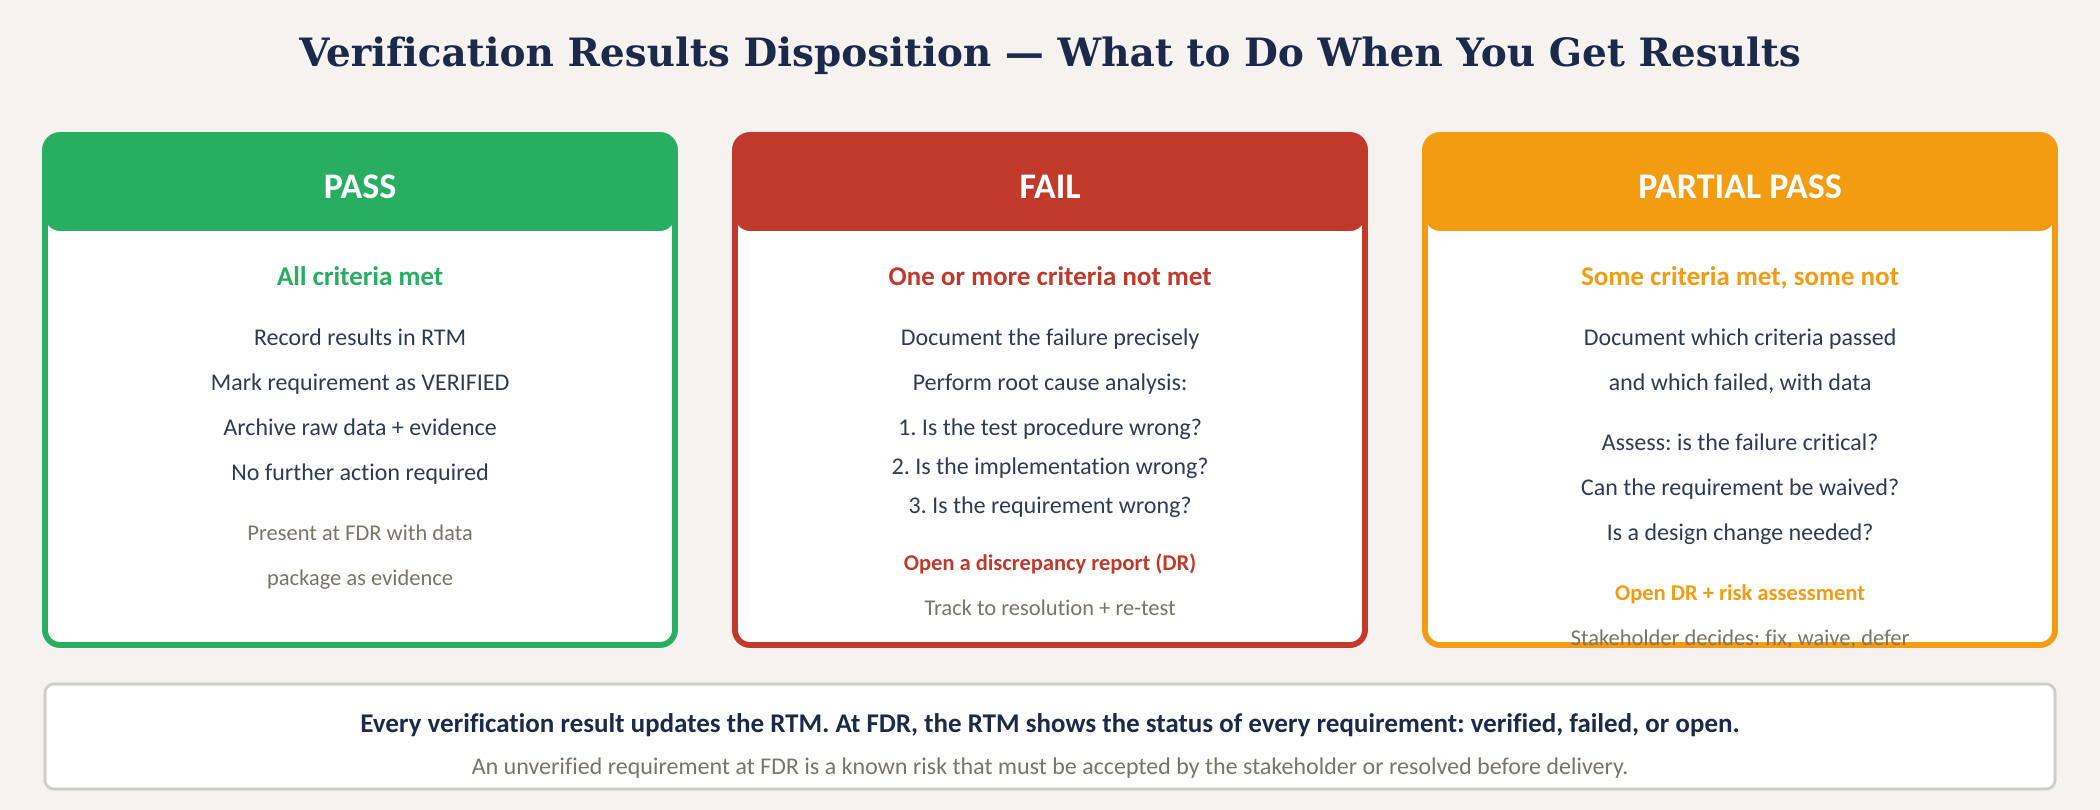
\includegraphics[width=\textwidth]{master_figs/fig_results_disposition.png}
\caption{Three verification outcomes: PASS, FAIL, PARTIAL PASS with disposition workflows.}\label{fig:disp}
\end{figure}

\subsection{PASS}
All criteria met. Record results in RTM, mark requirement VERIFIED, archive raw data. Include actual measurement values, not just ``PASS.''

\subsection{FAIL}
One or more criteria not met. Root cause analysis in order: (1) Is the test procedure wrong? (2) Is the implementation wrong? (3) Is the requirement wrong? Open a Discrepancy Report (DR), assign corrective action, track to resolution, re-test after correction.

\subsection{PARTIAL PASS}
Some criteria met, some not. Document which passed and which failed with data. Three resolution paths: \textbf{Fix} (redesign + re-test), \textbf{Waive} (stakeholder formally accepts the deviation with documented risk), or \textbf{Defer} (postpone with a plan and deadline). A waiver transfers risk to the stakeholder.

\subsection{Root Cause Analysis}
Three possible root causes, investigated in order: (1) the test is wrong (procedure error, calibration issue); (2) the implementation is wrong (most common); (3) the requirement is wrong (overly conservative or based on incorrect assumptions). Changing a requirement requires formal change control. Never silently.

\section{The VCRM}
The Verification Cross-Reference Matrix links every requirement to its method, procedure, and status. Maintain from day one. At FDR, it tells the complete story. Example columns: Req ID, Text, Type, Method, Test Proc ID, Status, Notes.


\subsection{VCRM Evolution Over Time}
The VCRM is not a static document; it evolves at each project milestone:
\begin{itemize}[nosep,leftmargin=1.5em]
\item \textbf{At PDR}: all requirements listed, methods assigned, status = ``Planned'' for all.
\item \textbf{At CDR}: some subsystem-level tests executed, status updated. Analysis-method requirements may show results from design calculations.
\item \textbf{At FDR}: all requirements have a final status. The VCRM is the single-page executive summary of your entire V\&V campaign.
\end{itemize}

\subsection{End-to-End Traceability Example}
\textbf{Stakeholder need}: ``I need to know when the greenhouse is too cold.'' $\to$ \textbf{System requirement}: SYS-REQ-003: ``The system shall send an SMS alert within 60\,s of heater activation.'' $\to$ \textbf{Verification method}: Test. $\to$ \textbf{Test procedure}: TP-003: Trigger heater activation, start stopwatch, verify SMS received within 60\,s, record actual time for 3 trials. $\to$ \textbf{Result}: Trial 1: 12\,s, Trial 2: 14\,s, Trial 3: 11\,s. Mean = 12.3\,s. Verdict: PASS (12.3 $<$ 60). $\to$ \textbf{VCRM entry}: SYS-REQ-003 | Test | TP-003 | PASS | 12.3\,s mean.

This chain, need $\to$ requirement $\to$ method $\to$ procedure $\to$ result $\to$ VCRM, is what ``requirements-driven design'' means in practice.

\section{V\&V and the V-Model}
The V-Model maps development phases (left side) to verification phases (right side): stakeholder needs $\leftrightarrow$ validation, system requirements $\leftrightarrow$ system testing, subsystem requirements $\leftrightarrow$ integration testing, component specs $\leftrightarrow$ unit testing. Implementation is at the bottom. Test planning happens on the LEFT side; design tests while writing requirements.


\section{Statistical Confidence and Test Rigor}
\subsection{Developmental Testing vs.\ Production Qualification}
How many times must you run a test? For \textbf{developmental testing} (MEGN~301): 3 repetitions minimum per test point. Report mean and range. For \textbf{production qualification} (industry): sample sizes from statistical requirements; typically $n \geq 30$ for parametric statistics, or MIL-STD-1916 sampling plans.

\subsection{Practical Implications for Student Projects}
Run each test 3 times, report all three values plus the mean, flag any result where the spread exceeds 20\% of the mean. Report measurement uncertainty: if your instrument resolution is 0.1\,\degC{} and your requirement is $\pm$0.5\,\degC{}, you have adequate measurement capability. If your instrument resolution is 0.5\,\degC{}, you cannot meaningfully verify a $\pm$0.5\,\degC{} requirement.


\subsection{The Test Environment Matters}
Test conditions that differ from operational conditions produce invalid results. Document and control: ambient temperature, humidity, power supply source (bench supply vs.\ battery vs.\ wall adapter; each behaves differently), electromagnetic environment (lab bench vs.\ field), and mechanical mounting (loose on bench vs.\ installed in enclosure). Any deviation from the intended operating environment must be noted in the test report with an assessment of impact.

\subsection{Measurement Uncertainty}
Every measurement has uncertainty. Your instrument's resolution, accuracy, and calibration status all contribute. Rule of thumb: the measurement system should be $\geq$4$\times$ more accurate than the requirement tolerance. If your requirement is $\pm$0.5\,\degC{}, your measurement system must be accurate to $\pm$0.125\,\degC{} or better. Document measurement uncertainty in every test report.

\section{Edge Case and Boundary Testing}
Requirements specify ranges (``0 to 50\,\degC{},'' ``0 to 100\% RH''). Test at: the \textbf{nominal} operating point, \textbf{both boundary values}, and at least one point \textbf{outside} the boundary to verify graceful degradation (not catastrophic failure).

\begin{tipbox}[The Room-Temperature Trap]
Testing only at room temperature ($\$\sim\$$22\,\degC{}) is the most common V\&V shortcut. If your requirement says 0--50\,\degC{}, you \emph{must} test at 0\,\degC{} and 50\,\degC{}. Use the ME department environmental chamber or an ice bath + heat gun. A system that works at 22\,\degC{} but fails at 0\,\degC{} does not meet the requirement.
\end{tipbox}

\section{Minimum Viable V\&V for MEGN 301}
The minimum V\&V package for student projects:
\begin{enumerate}[nosep,leftmargin=1.5em]
\item A VCRM with every requirement assigned a method and status.
\item A written test procedure (all 10 sections) for every T-method requirement.
\item Test results with actual measured data (not just ``pass'').
\item For FAIL or PARTIAL PASS: root cause analysis and corrective action.
\item Peer review: another team executes at least one procedure. If they cannot reproduce results, the procedure is inadequate.
\end{enumerate}

\section{External Team Testing}
Having another team execute your test procedures verifies reproducibility and uncovers ambiguities. \textbf{Preparing}: provide the procedure, equipment list, and safety briefing. Do NOT explain verbally; the document must stand alone. Observe without intervening (unless safety). Collect written feedback on every unclear step.

\begin{greenshieldbox}[GreenShield: VCRM Fragment at Three Milestones]
\small
\begin{tabularx}{\textwidth}{l l c c c}
\toprule
\textbf{Req ID} & \textbf{Requirement} & \textbf{Method} & \textbf{At PDR} & \textbf{At CDR} \\
\midrule
SYS-REQ-001 & Temp meas.\ at $\geq$1\,Hz & T & Planned & In Progress \\
SYS-REQ-002 & Heater at $\leq$setpoint & T & Planned & PASS \\
SYS-REQ-003 & SMS within 60\,s & T & Planned & Planned \\
SYS-REQ-004 & Autonomous mode on failure & D & Planned & Planned \\
SYS-REQ-005 & Accuracy $\pm$0.5\,\degC{} & T & Planned & PARTIAL \\
\bottomrule
\end{tabularx}

At \textbf{FDR}: all rows should show PASS, FAIL with Discrepancy Report, or waived with stakeholder approval. SYS-REQ-005 PARTIAL PASS (0.6\,\degC{} error at 0\,\degC{} boundary) requires resolution.
\end{greenshieldbox}

\begin{keyconceptbox}[Industry SE Parallels]
\begin{itemize}[nosep,leftmargin=1.5em]
\item \textbf{INCOSE SEH 4th ed.}: Sec.\ 4.10 (Verification), Sec.\ 4.11 (Validation).
\item \textbf{NASA SP-2016-6105 Rev 2}: Ch.\ 5.3 (Verification), Ch.\ 5.4 (Validation).
\item \textbf{IEEE 1012}: Standard for System, Software, and Hardware V\&V.
\end{itemize}
\end{keyconceptbox}

\section{Artifact Handoff: What Chapter 4 Produces}
\begin{table}[htbp]\centering\small
\begin{tabularx}{\textwidth}{l X l}
\toprule
\textbf{Artifact} & \textbf{Description} & \textbf{Forward Reference} \\
\midrule
VCRM & Cross-reference matrix linking reqs to test status & CDR, FDR deliverables \\
Test Procedures & Reproducible procedures for every T-method requirement & Ch.~5 (integration test) \\
Test Reports & Results with data, verdict, and any DRs & FDR documentation \\
\bottomrule
\end{tabularx}
\end{table}


\section{Statistical Confidence and Test Rigor}
How many times must you run a test? For \textbf{developmental testing} (MEGN~301): 3 repetitions minimum per test point. Report mean and range. For \textbf{production qualification}: sample sizes from statistical requirements ($n \geq 30$ for parametric statistics, or MIL-STD-1916 sampling plans).

For MEGN~301: run each test 3 times, report all three values plus the mean, flag any result where spread exceeds 20\% of mean.

\section{Edge Case and Boundary Testing}
Requirements specify ranges (``0 to 50\,\degC{}'', ``0 to 100\%\ RH''). Test at: the \textbf{nominal} operating point, \textbf{both boundary values}, and at least one point \textbf{outside} the boundary to verify graceful degradation.

\begin{tipbox}[The Room-Temperature Trap]
Testing only at 22\,\degC{} is the most common V\&V shortcut in student projects. If your requirement says 0--50\,\degC{}, you must test at 0\,\degC{} and 50\,\degC{}. Use the ME department environmental chamber or an ice bath + heat gun.
\end{tipbox}

\section{Minimum Viable V\&V for MEGN 301}
The minimum V\&V package:
\begin{enumerate}[nosep,leftmargin=1.5em]
\item A VCRM with every requirement assigned a method and status.
\item Written test procedures (all 10 sections) for every T-method requirement.
\item Test results with actual measured data (not just ``pass'').
\item For FAIL or PARTIAL PASS: root cause analysis and corrective action plan.
\item Peer review: another team executes at least one of your procedures.
\end{enumerate}

\section{External Team Testing}
Having another team execute your test procedures verifies reproducibility and uncovers ambiguities the authoring team is blind to.

\textbf{Preparation}: (1) Provide the procedure, equipment list, and safety briefing. (2) Do NOT explain verbally; the document must stand alone. (3) Observe without intervening (unless safety). (4) Collect written feedback on unclear steps.

\begin{greenshieldbox}[GreenShield: VCRM at Three Milestones]
\small
\begin{tabularx}{\textwidth}{l l c c c}
\toprule
\textbf{Req ID} & \textbf{Requirement} & \textbf{Method} & \textbf{CDR} & \textbf{FDR} \\
\midrule
SYS-001 & Temp at $\geq$1\,Hz & T & In Progress & PASS \\
SYS-002 & Heater at $\leq$ setpoint & T & PASS & PASS \\
SYS-003 & SMS within 60\,s & T & Planned & PASS \\
SYS-004 & Autonomous on comm fail & D & Planned & PASS \\
SYS-005 & Accuracy $\pm$0.5\,\degC{} & T & PARTIAL & PASS \\
\bottomrule
\end{tabularx}
\end{greenshieldbox}

\begin{keyconceptbox}[Industry SE Parallels]
\begin{itemize}[nosep,leftmargin=1.5em]
\item \textbf{INCOSE SEH 4th ed.}: \S4.10 Verification, \S4.11 Validation.
\item \textbf{NASA SP-2016-6105 Rev~2}: Ch.~5.3 Verification, Ch.~5.4 Validation.
\item \textbf{IEEE 1012}: System, Software, and Hardware V\&V.
\end{itemize}
\end{keyconceptbox}

\section{Artifact Handoff: What Chapter 4 Produces}
\begin{table}[htbp]\centering\small
\begin{tabularx}{\textwidth}{l X l}
\toprule
\textbf{Artifact} & \textbf{Description} & \textbf{Used In} \\
\midrule
VCRM & Reqs linked to test status & CDR, FDR \\
Test Procedures & Reproducible procedures for T-method reqs & Ch.~5 \\
Test Reports & Results with data, verdict, and DRs & FDR \\
\bottomrule
\end{tabularx}
\end{table}

\section{Test Method Selection: T-A-I-D}
Every requirement must be verified by one of four methods:

\textbf{Test (T)}: direct measurement of the parameter under controlled conditions. Most rigorous; provides quantitative evidence. Use for: performance requirements (accuracy, speed, power consumption), safety requirements (overcurrent protection, thermal shutdown), and environmental requirements (temperature range, vibration).

\textbf{Analysis (A)}: mathematical or computational evaluation. Use when testing is impractical (structural stress analysis before building, thermal simulation of extreme conditions, reliability prediction from component data). Analysis is only as good as the model; document all assumptions.

\textbf{Inspection (I)}: visual or dimensional examination. Use for: physical characteristics (weight, dimensions, color, marking), material identification (marked per specification), and workmanship (solder quality, wire routing, labeling).

\textbf{Demonstration (D)}: qualitative exercise of the system's functions without quantitative measurement. Use for: user interface verification (the display shows the correct information), operational procedures (the system starts up correctly), and safety demonstrations (the emergency stop works).

\textbf{Selection guideline}: use Test whenever feasible. Use Analysis when testing is impossible or prohibitively expensive. Use Inspection for attributes that can be directly observed. Use Demonstration for qualitative or pass/fail functions.

\section{Designing for Testability}
Design decisions made early in the project determine whether the system can be effectively tested:

\textbf{Test points}: include physical access points for measuring voltages, currents, and signals at key locations in the circuit. A test header (pin row connected to critical signals) allows an oscilloscope to be quickly attached during debugging and formal testing.

\textbf{Calibration access}: if the system requires calibration (sensor offset, gain adjustment, PID tuning), provide a software interface (serial command, button sequence, or configuration file) for entering calibration parameters without modifying firmware.

\textbf{Diagnostic modes}: firmware that can output raw sensor values, intermediate calculations, and actuator commands to a serial port enables rapid diagnosis of integration problems. Include a ``debug'' mode that bypasses the normal user interface and shows engineering-level data.

\textbf{Stimulus injection}: the ability to inject known test signals (simulated sensor readings, forced actuator commands) enables testing individual subsystems without the full system connected. In firmware, a ``simulation'' mode that replaces real sensor data with predefined test values is invaluable.

\section{Writing Test Procedures}
A test procedure must be detailed enough that someone who did not design the system can execute the test and obtain the same result. Each procedure includes:

\textbf{Objective}: what requirement is being verified, and what will be measured.

\textbf{Equipment}: list every instrument by type and calibration status (e.g., ``Fluke 87V DMM, Cal.\ due 2026-06-15'').

\textbf{Setup}: how to configure the system and instruments, including specific settings (DAQ range, sample rate, trigger mode).

\textbf{Procedure}: numbered steps. Each step is a single action: ``Set the power supply to 12.0\,V, current limit 2.0\,A.'' ``Record the temperature sensor reading in Table~1.'' ``Wait 60\,s for the system to reach steady state.''

\textbf{Data recording}: a pre-formatted table or form for recording results, including spaces for the tester's name, date, environmental conditions, and equipment serial numbers.

\textbf{Acceptance criteria}: the quantitative pass/fail threshold. ``PASS if the measured temperature is within $\pm$1.0\,\degC{} of the reference at all 5 setpoints. FAIL if any setpoint deviation exceeds 1.0\,\degC{}.''

\textbf{Safety}: any hazards and required precautions. ``High voltage present when cover is removed. Do not touch exposed terminals.''

\section{Failure Modes and Effects Analysis (FMEA)}
FMEA systematically identifies potential failure modes, their effects, and their causes, then prioritizes them for mitigation:

For each component or function: (1) how can it fail (failure mode)? (2) what happens to the system if it fails (effect)? (3) how severe is the effect (severity: 1--10)? (4) how likely is the failure (occurrence: 1--10)? (5) how likely is the failure to be detected before it causes harm (detection: 1--10)? (6) Risk Priority Number: $\text{RPN} = S \times O \times D$.

Prioritize mitigation actions for the highest RPNs. Common mitigations: redundancy (add a backup), derating (operate components below their maximum ratings), testing (detect failures before deployment), and design changes (eliminate the failure mode entirely).

In MEGN~301, a simplified FMEA covering the top 10 failure modes is expected in the CDR package. Focus on: safety-critical failures (fire, shock, mechanical injury), mission-critical failures (system cannot perform its primary function), and high-probability failures (connectors, batteries, moving parts).
\section{Practice Questions}
\begin{enumerate}[leftmargin=1.5em]
\item Explain how a system can pass all verification tests but fail validation. Give a concrete example.
\item Classify each requirement by verification method (T/A/I/D): (a) ``Shall withstand 50\,N load without permanent deformation.'' (b) ``Shall display the company logo on the front panel.'' (c) ``Shall complete a power-on sequence within 10 seconds.'' (d) ``Shall have a thermal margin of $\geq$20\,$^{\circ}$ C at max power under worst-case ambient.''
\item Write a complete test procedure (all 9 sections) for verifying: ``SYS-REQ-007: The system shall measure ambient temperature with accuracy of $\pm$0.5\,$^{\circ}$ C over 0 to 50\,$^{\circ}$ C.''
\item A test result shows 0.6\,$^{\circ}$ C error against a requirement of $\pm$0.5\,$^{\circ}$ C. What is the verdict? Describe the three possible root causes and the investigation sequence.
\item Your VCRM shows 18 PASS, 2 FAIL, and 1 PARTIAL PASS out of 21 requirements at FDR. What do you present to the stakeholder?
\end{enumerate}

\subsection{Answers}
\begin{enumerate}[leftmargin=1.5em]
\item A greenhouse monitoring system meets all temperature accuracy, data rate, and communication requirements (verified). But the stakeholder discovers the display is unreadable in direct sunlight; a need that was never captured as a requirement. The system was built right (verification), but it was not the right system (validation failed). This is a requirements-capture failure.
\item (a) Test; apply 50\,N load and measure deformation. (b) Inspection; visually confirm logo presence and placement. (c) Demonstration; power on and time the sequence. (d) Analysis; thermal simulation under worst-case conditions.
\item Purpose: verifies SYS-REQ-007. Setup: NIST-traceable temperature bath ($\pm$0.05\,$^{\circ}$ C), calibrated reference thermometer, DUT powered and warmed 30 min. Preconditions: DUT firmware v2.1, ambient 23$\pm$3\,$^{\circ}$ C. Steps: (1) Set bath to 0.0\,$^{\circ}$ C, wait 10 min, record DUT and reference. (2) Repeat at 10, 20, 30, 40, 50\,$^{\circ}$ C. Pass/fail: $|$DUT $-$ reference$|$ $\leq$ 0.5\,$^{\circ}$ C at every point. Data: table with columns for setpoint, reference, DUT, error. Safety: bath uses water, standard lab PPE. Signatures: tester, witness, date.
\item Verdict: FAIL (0.6 $>$ 0.5). Investigation: (1) Check test: was the reference bath stable? Was the reference thermometer calibrated? Repeat with verified equipment. (2) Check implementation: sensor calibration coefficients, ADC linearity, thermal coupling. (3) Check requirement: was $\pm$0.5\,$^{\circ}$ C justified? If the application can tolerate $\pm$1.0\,$^{\circ}$ C, a requirements change (with stakeholder approval) may be appropriate. Open a DR regardless.
\item Present the VCRM showing all 21 requirements with status. For the 18 PASS items, show evidence summaries. For the 2 FAIL items, present root cause analysis, corrective actions, and re-test plan with timeline. For the PARTIAL PASS, present which criteria passed, which failed, risk assessment, and recommendation (fix, waive, or defer). The stakeholder decides on the partial pass and accepts or rejects the open items.
\end{enumerate}


\subsection{Answers (continued)}
\begin{enumerate}[leftmargin=1.5em, start=6]
\item \textbf{External testing value}: When your team writes and executes its own test procedures, you unconsciously fill in gaps with tacit knowledge (``oh, you need to wait 30 seconds after power-on before reading the sensor'', but the procedure does not say that). An external team has no tacit knowledge. Every ambiguity, missing step, and unclear criterion is exposed. The external team's feedback is a direct measure of your documentation quality.

\item \textbf{Boundary testing strategy}: For a requirement ``0--50\,\degC{} $\pm$0.5\,\degC{}'': test at 0\,\degC{} (boundary), 25\,\degC{} (nominal), and 50\,\degC{} (boundary). Also test at $-5$\,\degC{} and 55\,\degC{} to verify graceful degradation (system should report out-of-range, not crash or give false readings). For humidity requirement ``0--100\% RH'': test at 0\% (desiccant chamber), 50\% (ambient), and 95\% (humidity chamber; 100\% causes condensation that is a separate failure mode). Report all data points, not just pass/fail.
\end{enumerate}

\chapter{Subsystem Integration}

\vspace{1em}
\vspace{1em}

\begin{figure}[htbp]\centering
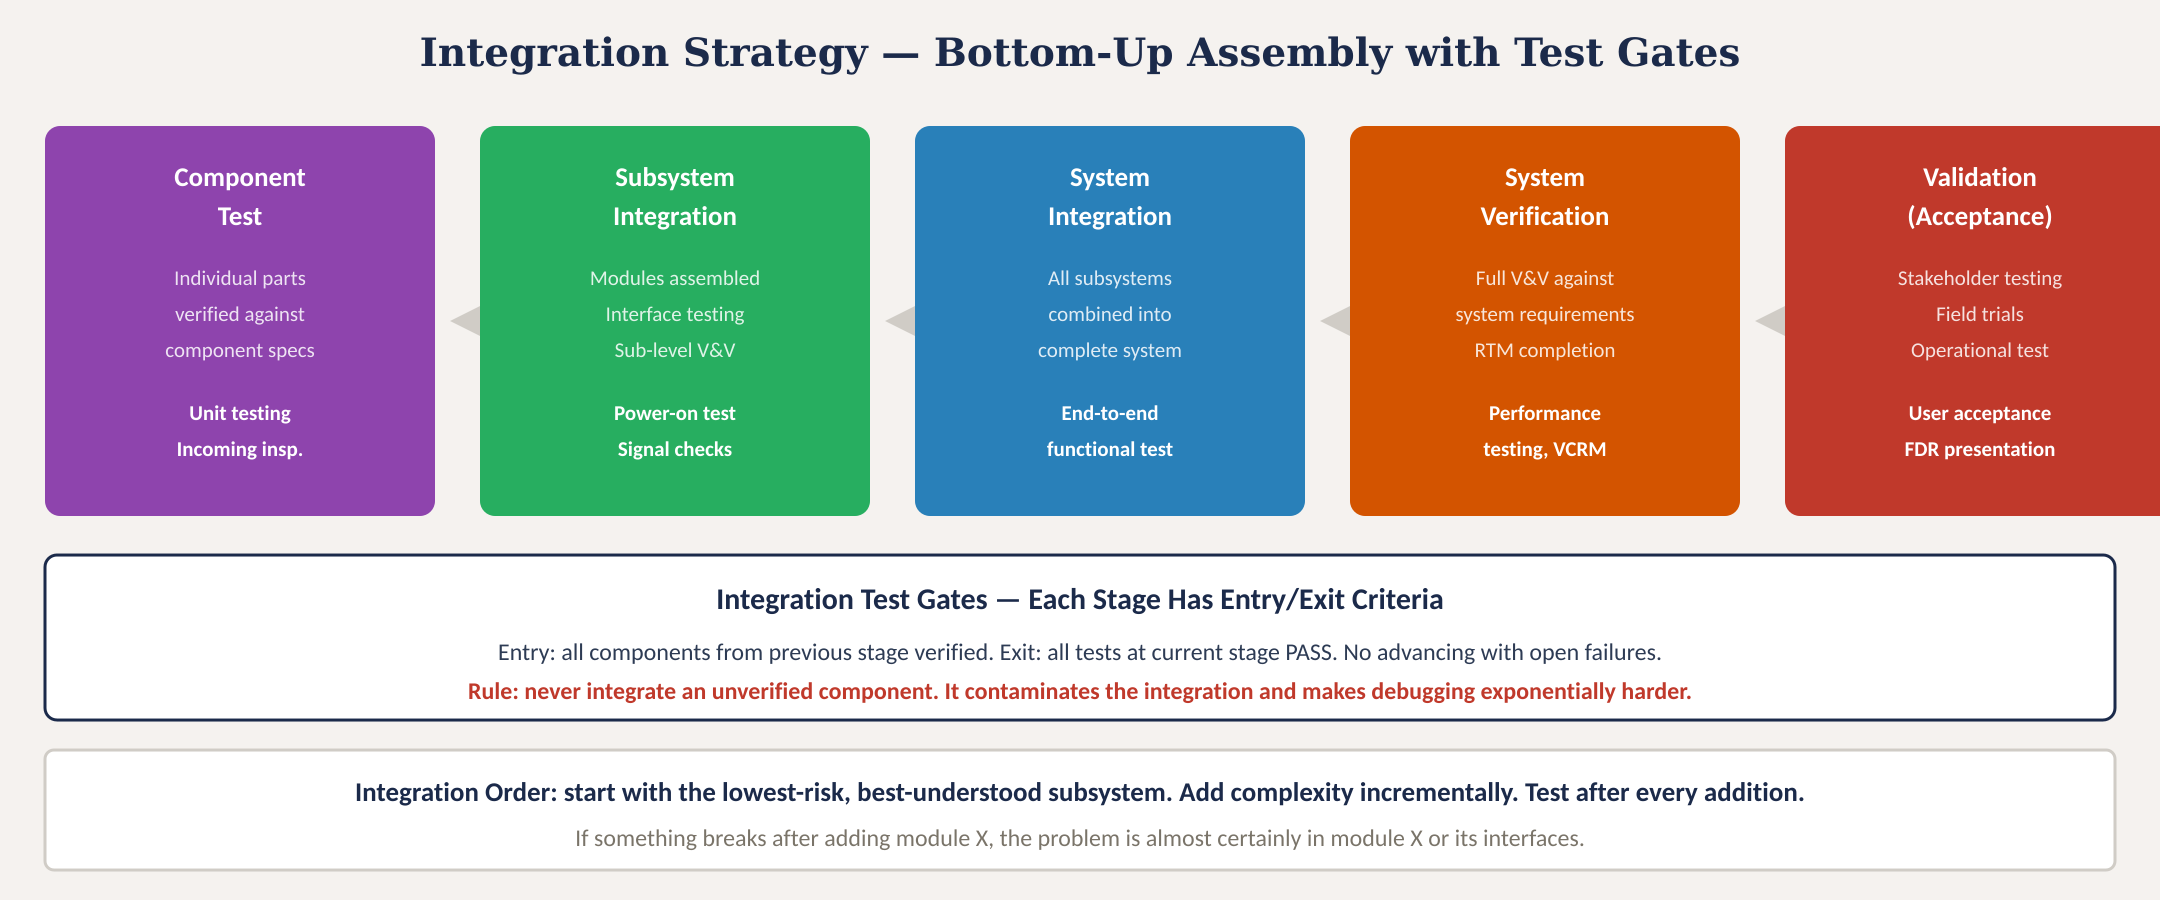
\includegraphics[width=\textwidth]{master_figs/fig_integration_strategy.png}
\caption{Bottom-up integration with test gates.}\end{figure}

\begin{figure}[htbp]\centering
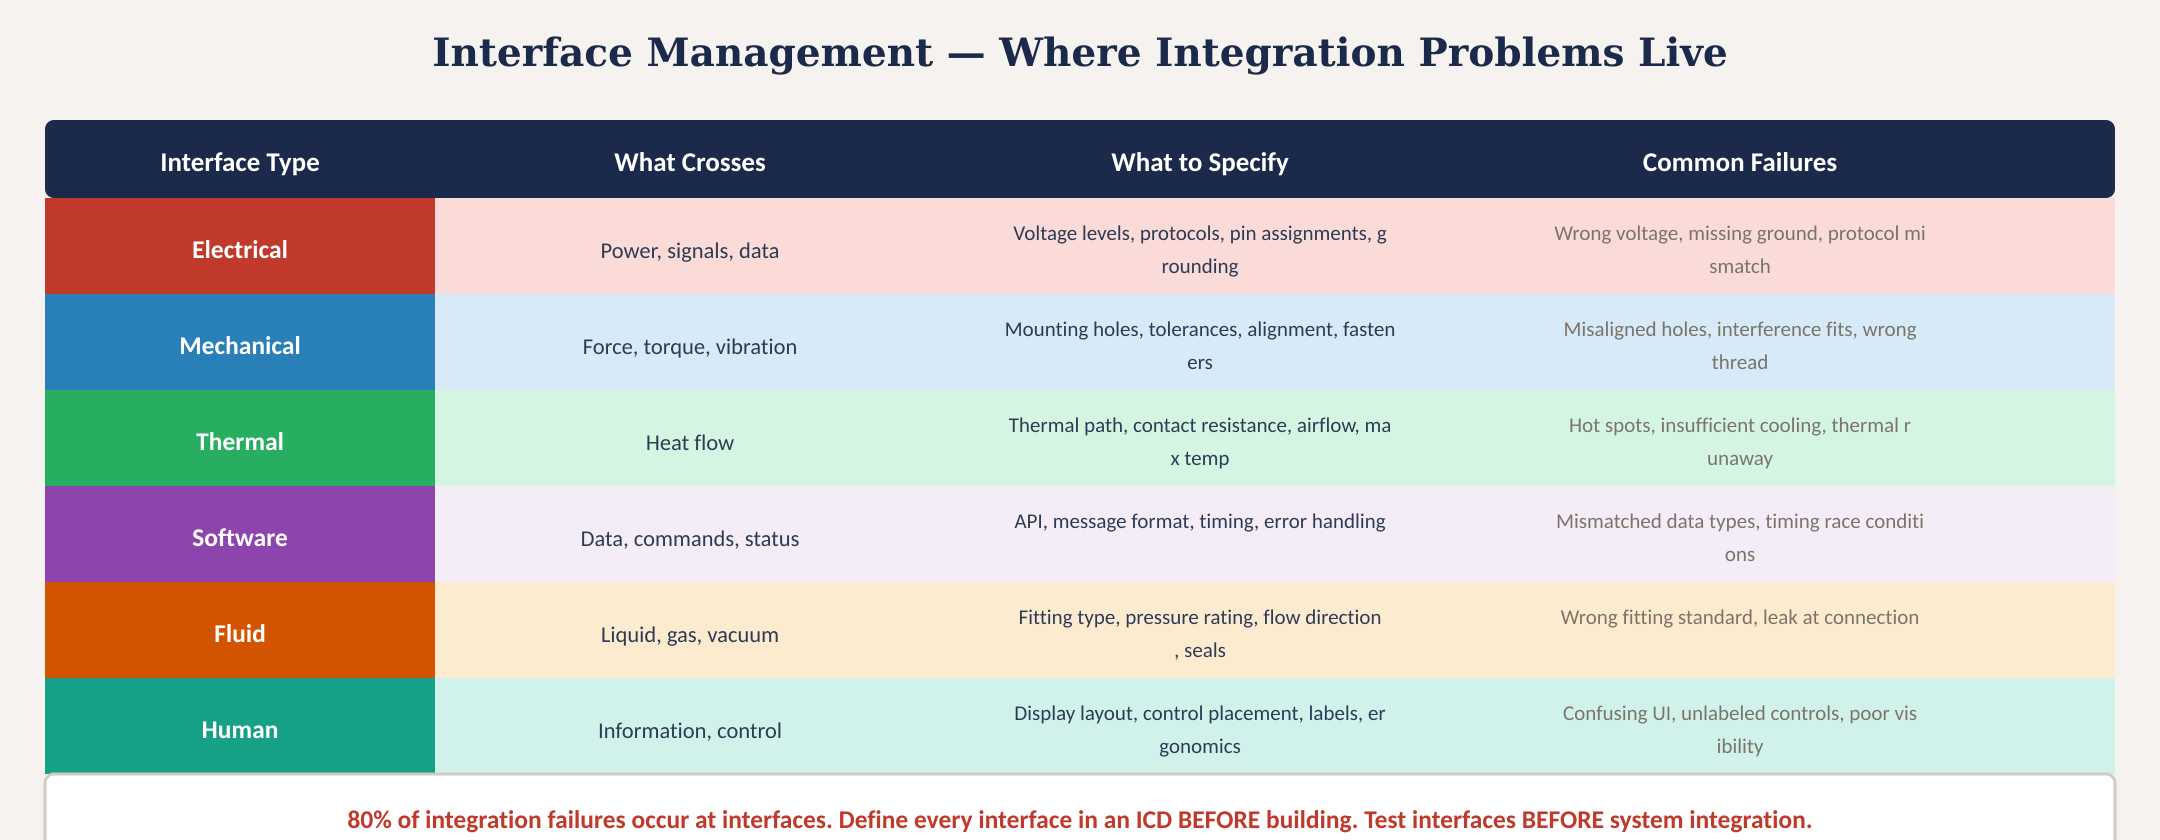
\includegraphics[width=\textwidth]{master_figs/fig_interface_management.png}
\caption{Interface types and common failure modes.}\end{figure}

\begin{figure}[htbp]\centering
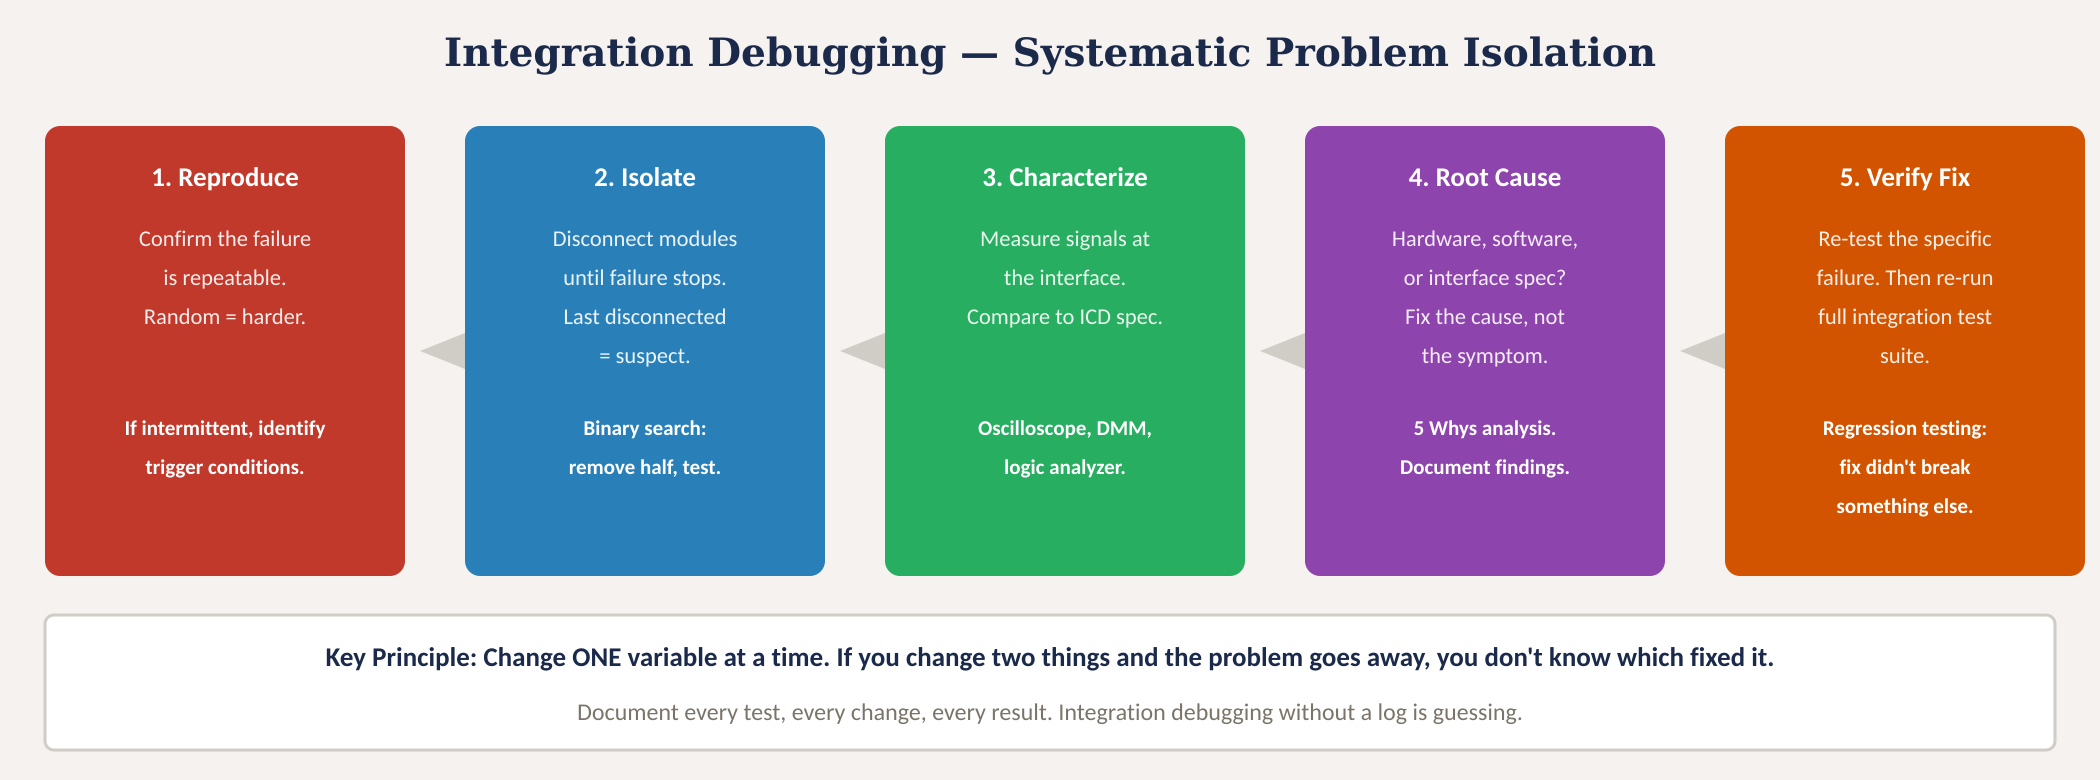
\includegraphics[width=\textwidth]{master_figs/fig_debugging_process.png}
\caption{Five-step systematic debugging process.}\end{figure}

\begin{figure}[htbp]\centering
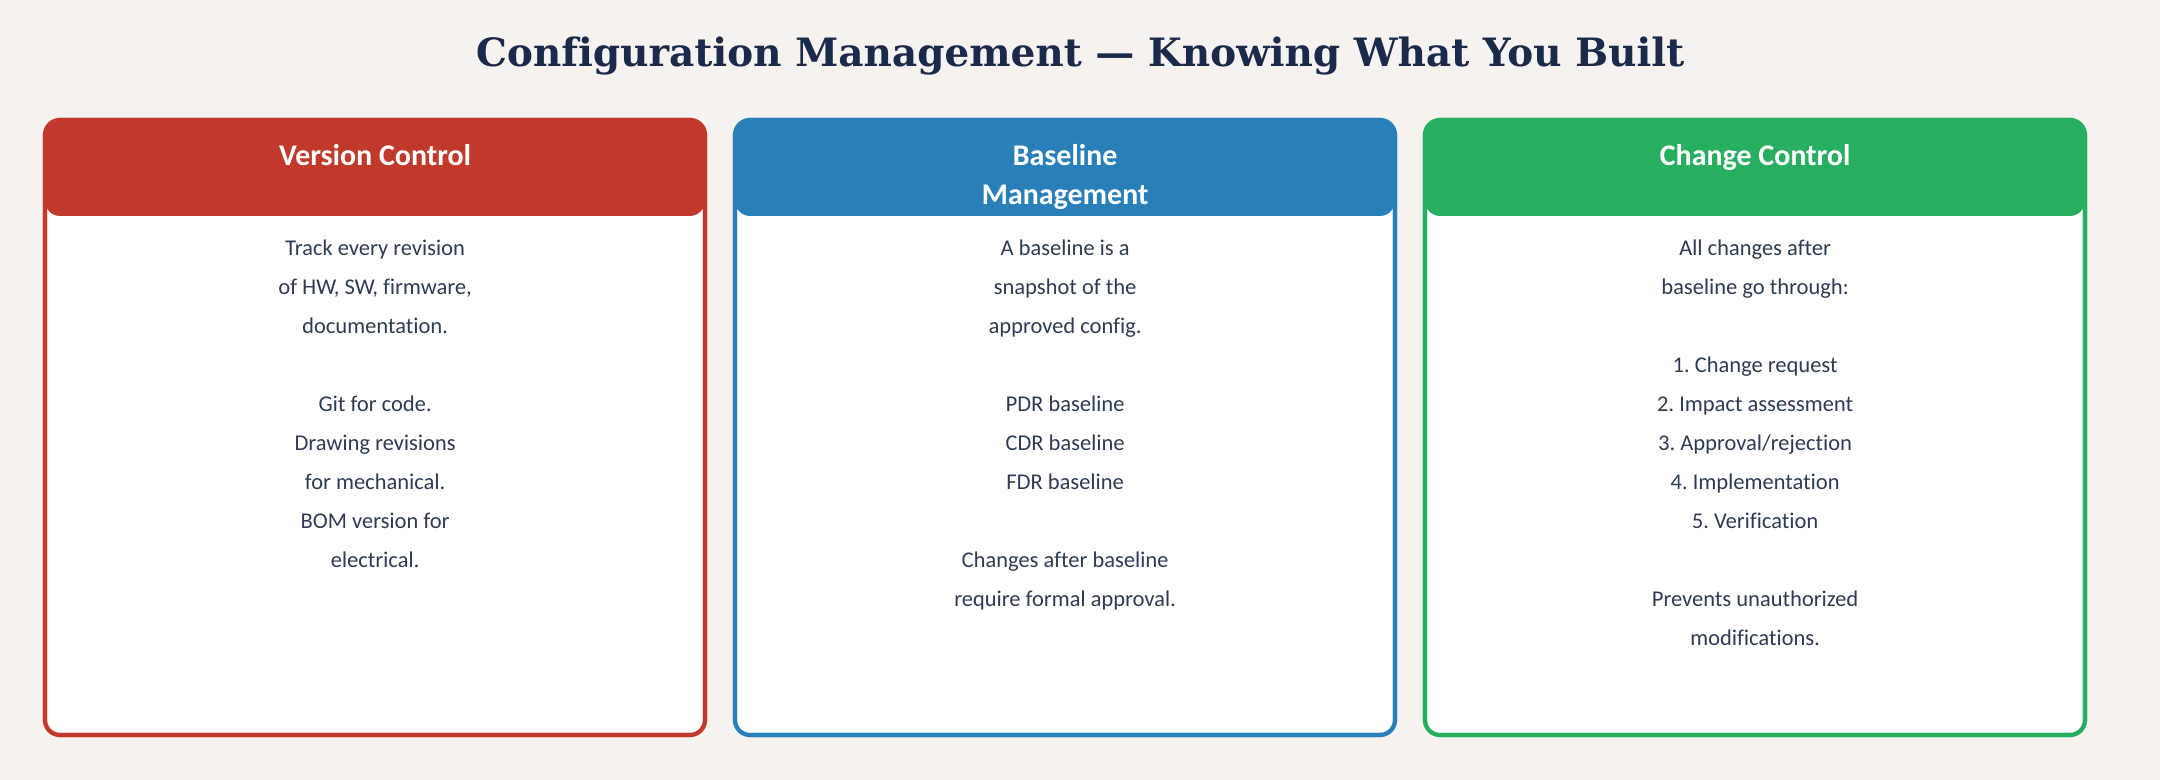
\includegraphics[width=\textwidth]{master_figs/fig_config_management.png}
\caption{Configuration management pillars.}\end{figure}

\section{Integration Strategy}
\subsection{Bottom-Up Integration}
Verify components individually $\to$ integrate into subsystems $\to$ test each subsystem $\to$ combine into system $\to$ system test. At each stage, add ONE new element and test. If something breaks, the new element or its interface is the suspect. \textbf{Never big-bang} (assemble everything at once).


\subsection{Integration Stages and the V-Model}
The V-Model maps integration from bottom-up: \textbf{Component verification} (each part works alone), \textbf{Subsystem integration} (components within a subsystem work together), \textbf{System integration} (subsystems work together), \textbf{System verification} (system meets all requirements), \textbf{Validation} (system meets stakeholder needs). Each stage has specific entry and exit criteria. Never advance with open failures.

\subsection{Integration Sequence Planning}
The order of integration matters. Rules: (1) Integrate power first; nothing works without power. (2) Add the lowest-risk subsystem next. (3) Add the highest-risk subsystem last (so problems are isolated to one new element). (4) Never add two new elements simultaneously (if something breaks, you cannot isolate the cause).

\subsection{Test Gates}
Each integration stage has entry and exit criteria. Entry: all components from the previous stage verified. Exit: all tests at the current stage PASS. Never advance with open failures.


\subsection{Critical Subsystem Demonstrations}
Before full system integration, each subsystem must pass a standalone demonstration. Three steps: (1)~\textbf{Plan}; define pass/fail criteria, (2)~\textbf{Execute}; run with data recording (video for design review), (3)~\textbf{Document}; 1-page summary with data, photos, verdict. This is a CDR deliverable.

\subsection{The N\textsuperscript{2} (N-Squared) Diagram}
The N\textsuperscript{2} diagram maps interfaces between subsystems. Modules on the diagonal; cell $(i,j)$ = what module $i$ sends to module $j$. Dense rows/columns = high integration risk.

\begin{greenshieldbox}[GreenShield: N\textsuperscript{2} Diagram (5$\times$5)]
\small
\begin{tabularx}{\textwidth}{l|c|c|c|c|c}
 & \textbf{Sensor} & \textbf{MCU} & \textbf{Relay} & \textbf{Comms} & \textbf{PSU} \\
\hline
\textbf{Sensor} & --- & Temp (I2C) & & & \\
\hline
\textbf{MCU} & Config & --- & GPIO & UART TX & \\
\hline
\textbf{Relay} & & Status & --- & & \\
\hline
\textbf{Comms} & & UART RX & & --- & \\
\hline
\textbf{PSU} & 3.3V & 3.3V & 12V & 3.3V &; \\
\end{tabularx}

PSU interfaces with everything. MCU receives from everything. Both are high-risk integration points. The I2C bus requires defined pull-up resistor ownership.
\end{greenshieldbox}

\begin{greenshieldbox}[GreenShield: I\textsuperscript{2}C Pull-Up Failure]
The sensor team assumed the MCU board had pull-ups. The MCU team assumed the sensor breakout had them. Neither did. I2C floated, communication was intermittent, 8 hours of debugging. \textbf{Fix}: every ICD must state which side provides pull-ups, termination resistors, and bias voltages.
\end{greenshieldbox}

\begin{tipbox}[Case Study: Diagnosing Brown-Out Blues]
A greenhouse controller reset randomly on relay activation. Scope showed 800\,mV dip on 3.3\,V rail (below 2.7\,V brown-out threshold). Root cause: relay coil inrush through shared power trace. Fix: 470\,$\mu$F cap on MCU rail + separate relay power trace. Regression: 100 relay cycles, zero resets.
\end{tipbox}

\begin{keyconceptbox}[Industry SE Parallels]
\begin{itemize}[nosep,leftmargin=1.5em]
\item \textbf{INCOSE SEH 4th ed.}: \S4.6 Implementation, \S4.7 Integration.
\item \textbf{NASA SP-2016-6105 Rev~2}: Ch.~5.1 Implementation, Ch.~5.2 Integration.
\end{itemize}
\end{keyconceptbox}

\section{Artifact Handoff: What Chapter 5 Produces}
\begin{table}[htbp]\centering\small
\begin{tabularx}{\textwidth}{l X l}
\toprule
\textbf{Artifact} & \textbf{Description} & \textbf{Used In} \\
\midrule
Integration Plan & Build sequence with test gates & CDR \\
N\textsuperscript{2} Diagram & Interface matrix & ICD verification \\
Integration Test Results & Subsystem and system-level data & FDR \\
\bottomrule
\end{tabularx}
\end{table}

\section{Interface Management}
80\% of integration failures occur at interfaces. Six types: electrical (voltage, protocols, grounding), mechanical (mounting, tolerances, alignment), thermal (heat flow, contact resistance), software (APIs, data formats, timing), fluid (fittings, pressure, seals), and human (displays, controls, ergonomics).

Write Interface Control Documents (ICDs) DURING architecture — not during integration. The ICD defines what crosses each boundary, in what format, with what constraints. Every interface needs a single owner.


\subsection{Interface Control Documents (ICDs)}
An ICD defines what crosses each boundary, in what format, with what constraints. Minimum ICD content for each interface:
\begin{enumerate}[nosep,leftmargin=1.5em]
\item \textbf{Interface name and number} (e.g., ICD-003: MCU $\leftrightarrow$ Relay Driver).
\item \textbf{Physical connection}: connector type, pin assignments, wire gauge/color.
\item \textbf{Electrical characteristics}: voltage levels, current draw, impedance, timing.
\item \textbf{Protocol}: I2C address, baud rate, message format, error handling.
\item \textbf{Ownership}: which side provides power, pull-ups, termination.
\item \textbf{Test method}: how you verify the interface works (oscilloscope measurement, loopback test).
\end{enumerate}

Every ICD must be signed by the owners of both sides of the interface. Unsigned ICDs are the \#1 root cause of integration failures.

\section{Debugging}
Five-step process: (1) Reproduce the failure reliably. (2) Isolate by disconnecting modules until the failure stops. (3) Characterize by measuring signals at the interface against the ICD. (4) Root-cause: hardware, software, or interface spec? (5) Verify the fix, then regression-test. \textbf{Change ONE variable at a time.}

\section{Configuration Management}
Three pillars: \textbf{Version control} (Git for code, revision letters for drawings, versioned BOMs), \textbf{Baseline management} (PDR/CDR/FDR snapshots with formal change control after baseline), \textbf{Change control} (change request $\to$ impact assessment $\to$ approval $\to$ implementation $\to$ verification).


\subsection{Critical Subsystem Demonstrations}
Before full integration, each subsystem should pass a standalone demonstration. Three steps: (1) \textbf{Plan}: define what the subsystem demonstrates, test equipment needed, pass/fail criteria. (2) \textbf{Execute}: run the demonstration with data recording; video for design review. (3) \textbf{Document}: 1-page summary with data, photos, verdict; a CDR deliverable.

\subsection{The N\textsuperscript{2} (N-Squared) Diagram}
The N\textsuperscript{2} diagram maps interfaces between subsystems. Modules on the diagonal; cell $(i,j)$ describes what module $i$ sends \emph{to} module $j$. Empty cells = no interface. Dense rows = high-integration-risk modules.

Building one: list modules on the diagonal; for each pair ask ``does module $i$ send anything to $j$?''; fill in signal type, protocol, voltage, data rate.

\begin{greenshieldbox}[GreenShield: N\textsuperscript{2} Diagram]
\small
\begin{tabularx}{\textwidth}{l|c|c|c|c|c}
 & \textbf{Sensor} & \textbf{MCU} & \textbf{Relay} & \textbf{Comms} & \textbf{PSU} \\
\hline
\textbf{Sensor} & --- & Temp (I2C) & & & \\
\hline
\textbf{MCU} & Config & --- & GPIO high/low & UART TX & \\
\hline
\textbf{Relay} & & Status (GPIO) & --- & & \\
\hline
\textbf{Comms} & & UART RX & & --- & \\
\hline
\textbf{PSU} & 3.3V & 3.3V & 12V & 3.3V &; \\
\end{tabularx}

PSU row is dense (interfaces with everything). MCU column is dense (receives from everything). Both are high-risk integration points. The I2C interface between Sensor and MCU requires defined pull-up ownership.
\end{greenshieldbox}

\begin{greenshieldbox}[GreenShield: Integration Failure: I\textsuperscript{2}C Pull-Up Error]
The sensor team assumed the MCU board provided I2C pull-ups. The MCU team assumed the breakout board had them. Neither did. Result: bus floated, intermittent communication, 8 hours of debugging.

\textbf{Root cause}: ICD did not specify pull-up ownership. \textbf{Fix}: every ICD must explicitly state which side provides pull-ups, termination resistors, and bias voltages.
\end{greenshieldbox}

\begin{tipbox}[Case Study: Diagnosing the Brown-Out Blues]
A greenhouse controller worked on the bench but reset randomly in the field. Debugging: (1) Reproduced only when relay switched on. (2) Isolated: relay disconnected = stable. (3) Characterized: oscilloscope showed 800\,mV dip on 3.3\,V rail at relay switch-on. (4) Root cause: relay coil inrush drew 150\,mA through shared trace, drooping MCU supply below brown-out threshold. (5) Fix: 470\,$\mu$F cap on MCU rail, separate relay power trace. Regression: 100 relay cycles, zero resets.
\end{tipbox}

\begin{keyconceptbox}[Industry SE Parallels]
\begin{itemize}[nosep,leftmargin=1.5em]
\item \textbf{INCOSE SEH 4th ed.}: Sec.\ 4.6 (Implementation), Sec.\ 4.7 (Integration).
\item \textbf{NASA SP-2016-6105 Rev 2}: Ch.\ 5.1 (Product Implementation), Ch.\ 5.2 (Product Integration).
\end{itemize}
\end{keyconceptbox}

\section{Artifact Handoff: What Chapter 5 Produces}
\begin{table}[htbp]\centering\small
\begin{tabularx}{\textwidth}{l X l}
\toprule
\textbf{Artifact} & \textbf{Description} & \textbf{Forward Reference} \\
\midrule
Integration Plan & Build sequence, test gates, interface test list & CDR deliverable \\
N\textsuperscript{2} Diagram & Interface matrix with signal/power definitions & ICD verification \\
Integration Test Results & Subsystem and system-level test data & Ch.~4 (VCRM), FDR \\
\bottomrule
\end{tabularx}
\end{table}

\section{The Integration Challenge}
Subsystem integration is where student projects most commonly fail. Each subsystem may work perfectly on the bench in isolation, but when connected together, unexpected interactions emerge: electrical noise from the motor corrupts sensor readings, the mechanical frame flexes under load and misaligns optical sensors, the firmware timing that worked with one sensor fails when three sensors share the same bus, and the power supply that was adequate for bench testing sags under full system load.

The root cause is almost always insufficient interface definition during design. If the interfaces between subsystems are not precisely specified (voltage levels, timing, mechanical tolerances, thermal limits, EMI emissions), integration becomes a process of discovering and fixing problems rather than a planned assembly.

\section{Integration Order Strategy}
\textbf{Bottom-up integration}: build and test the lowest-level components first, then assemble them into subsystems, then integrate subsystems into the full system. Advantages: problems are isolated early. Disadvantages: the full system is not tested until the end.

\textbf{Top-down integration}: start with the system-level controller and add subsystems one at a time, using stubs (simulated inputs/outputs) for subsystems not yet available. Advantages: the system architecture is validated early. Disadvantages: stubs may not represent real subsystem behavior.

\textbf{Recommended for MEGN~301}: a hybrid approach. First, integrate the ``backbone'' (power supply + MCU + communication bus). Then add subsystems one at a time, testing each integration point before adding the next. If a problem appears, it is in the most recently added subsystem or its interface.

\section{Interface Verification}
Before connecting two subsystems, verify each interface independently:

\textbf{Electrical interfaces}: measure the voltage, current, impedance, and timing at each connection point. Verify that the driving subsystem can supply what the receiving subsystem requires. Check for voltage level compatibility (3.3\,V logic vs.\ 5\,V logic), current capacity (the source can provide the load's peak current), and signal integrity (rise time, ringing, overshoot within limits).

\textbf{Mechanical interfaces}: verify that mating features align within tolerance. Check that fastener holes are concentric, that press-fit dimensions match, and that there is clearance for wire routing and assembly tools. A 0.5\,mm misalignment that is invisible on the CAD screen becomes a show-stopper during assembly.

\textbf{Software interfaces}: verify that data formats, communication protocols, timing, and error handling are consistent between subsystems. A common failure: one subsystem sends data as a 16-bit signed integer while the other expects a 32-bit float.

\section{Integration Testing Protocol}
After each subsystem is connected, execute a focused integration test:

(1) \textbf{Smoke test}: power on and verify no component overheats, no magic smoke escapes, and no fuses blow. Seriously: this catches reversed power connections, short circuits, and overcurrent conditions before they cause damage.

(2) \textbf{Communication test}: verify that the newly connected subsystem can exchange data with the controller. Send a known command; verify the expected response.

(3) \textbf{Functional test}: exercise the subsystem through its full operating range while monitoring all other subsystems for interference. Does the motor's EMI corrupt the temperature sensor? Does the pump's vibration affect the accelerometer?

(4) \textbf{Document}: record the test results, any anomalies, and the system configuration (firmware version, wiring, component values).

\section{Debugging During Integration}
When something does not work after integration, resist the urge to change multiple things simultaneously. Instead:

\textbf{Isolate}: disconnect the newly added subsystem. Does the problem persist? If yes: the problem was pre-existing (regression). If no: the problem is in the new subsystem or its interface.

\textbf{Bisect}: for the new subsystem, test each interface signal independently. Is the power supply correct? Is the communication working? Is the sensor reading plausible? Is the actuator responding?

\textbf{Instrument}: add measurement points (oscilloscope probes, serial print statements, LED indicators) to observe internal signals. The problem is almost always at an interface, and measuring the interface signals identifies which side is at fault.

\begin{warningbox}[The Integration Time Estimate]
Students consistently underestimate integration time. A common estimate: ``we have 5 subsystems, each takes 1 day to build, so we need 5 days.'' Reality: building takes 5 days, but integration and debugging takes 5--15 more days. Budget at least 30\% of the total project time for integration and testing. If you have 15 weeks, reserve weeks 10--15 for integration, testing, and FDR preparation.
\end{warningbox}
\section{Configuration Management}
As the system evolves through integration and testing, keeping track of what changed, when, and why becomes critical. Configuration management (CM) practices prevent the chaos of ``I thought you changed that back'' and ``which firmware version is on this board?''

\textbf{Version control}: use a Git repository for all firmware, CAD files, and documentation. Every change has a commit message explaining what was changed and why. You can always revert to a previous version if a change introduces a problem.

\textbf{Hardware configuration log}: maintain a physical logbook (or spreadsheet) recording every hardware change: ``2026-03-15: Replaced R7 from 10k to 4.7k to fix gain error. ADN.'' Include the date, the change, the reason, and the person's initials. This log is invaluable when debugging: ``the system worked Tuesday but not Wednesday'' becomes a solvable problem if you know what changed between Tuesday and Wednesday.

\textbf{Build configuration tag}: when you have a known-good system configuration (hardware + firmware + calibration), tag it. Label the hardware (tape a note: ``Config v2.3, 2026-03-15''), tag the Git repository (``git tag v2.3''), and note the calibration date. If a change breaks something, you can revert to the tagged configuration.

\section{Interface Testing}
Before connecting two subsystems, verify each interface independently using loopback testing:

\textbf{Serial (UART) loopback}: connect TX to RX on the same device. Send a known string; verify it is received correctly. This confirms the baud rate, data format, and driver are correct before connecting to the other device.

\textbf{I2C bus scan}: use the Arduino ``I2C Scanner'' sketch to verify that each I2C device on the bus responds at the expected address. Missing devices indicate wiring errors or address conflicts.

\textbf{SPI echo}: send a known byte sequence to the SPI slave and read back the response. Verify the clock polarity, phase, and bit order match the slave's requirements.

\textbf{Power rail verification}: before connecting any subsystem to the power bus, measure the voltage and verify it is within the subsystem's input range. A 5\,V subsystem connected to a 12\,V rail is instantly destroyed.

\section{Integration Sequence for a Typical GreenShield Project}
Week 10: \textbf{Power system integration.} Connect the power supply to the distribution board. Verify all voltage rails. Connect the MCU and verify it boots. This is the ``backbone'' that everything else depends on.

Week 11: \textbf{Sensor integration.} Connect each sensor one at a time. For each: verify the raw ADC reading is plausible, apply the calibration equation, verify the engineering-unit output matches a reference measurement. If a sensor produces garbage data: check wiring, check the analog input mode (differential vs.\ RSE), check the ADC channel assignment in firmware.

Week 12: \textbf{Actuator integration.} Connect each actuator one at a time. For each: command a known output (50\% PWM, fixed valve position), verify the physical response (motor spins, heater heats, valve opens). If an actuator does not respond: check the drive circuit (MOSFET gate voltage, relay coil current), check the firmware output pin assignment, verify the power supply can handle the load.

Week 13: \textbf{Control loop closure.} Connect the sensor feedback to the controller. Start with conservative gains ($K_p$ at 20\% of expected value, $K_i = 0$, $K_d = 0$). Verify the loop responds in the correct direction (negative feedback: increasing temperature reduces heater power). If the loop runs away (positive feedback): the sensor polarity or the control sign is inverted. Gradually increase gains while monitoring stability.

Week 14: \textbf{System-level testing.} Execute the formal test plan. Document results. Address non-conformances.

Week 15: \textbf{FDR preparation.} Compile test results, finalize documentation, rehearse the presentation.
\section{Practice Questions}
\begin{enumerate}[leftmargin=1.5em]
\item Your system works with subsystems A and B connected, but fails when you add subsystem C. Describe your debugging approach step by step.
\item List all interfaces for a system with a sensor module, controller board, motor driver, and power supply. Which interfaces are highest risk?
\item Your teammate changes the firmware without telling anyone and the system stops working. What configuration management failure occurred?
\item Write entry and exit criteria for the subsystem integration stage of a greenhouse monitoring system.
\item Draw an N\textsuperscript{2} diagram for a system with four modules: temperature sensor, ESP32 MCU, relay driver, and OLED display. Identify the highest-risk interface and explain why.
\item Your team skipped critical subsystem demonstrations at CDR. During integration, the motor driver outputs 5\,V logic but the MCU expects 3.3\,V. What process failure caused this, and how would a proper ICD have prevented it?
\end{enumerate}

\subsection{Answers}
\begin{enumerate}[leftmargin=1.5em]
\item Debugging approach: (1) Reproduce: confirm failure occurs with A+B+C but not A+B. (2) Isolate: is it C itself or the C-to-A/C-to-B interface? Disconnect C from B, connect only C-to-A. Does it work? Then C-to-B interface is the suspect. (3) Characterize: measure signals at the C-to-B interface against the ICD. Check voltage levels, timing, protocol. (4) Root cause: is the interface spec wrong, or is C's output wrong? (5) Fix the specific issue, re-test, then add B back.
\item Interfaces: Sensor$\leftrightarrow$Controller (I2C data + power), Controller$\leftrightarrow$Motor Driver (PWM signal + power), Motor Driver$\leftrightarrow$PSU (high-current power), Controller$\leftrightarrow$PSU (logic power), Sensor$\leftrightarrow$PSU (sensor power). Highest risk: Controller$\leftrightarrow$Motor Driver (PWM noise coupling, ground bounce from motor current spikes) and Motor Driver$\leftrightarrow$PSU (inrush current, ground loops).
\item Configuration management failure: no change control process. The teammate made an uncontrolled change. Fix: establish version control (Git for firmware), require peer review before merge, tag releases, and never deploy untested code to the integration hardware.
\item Entry criteria: all subsystem tests passed, all ICDs signed, all subsystem firmware at tagged release, test equipment available. Exit criteria: all subsystem-to-subsystem interface tests pass, system powers up and executes basic sequence, no brown-out or reset events in 30-minute soak test.
\item N$^2$ diagram: MCU column is densest (receives from all three others). MCU$\leftrightarrow$Relay Driver interface is highest risk because it crosses voltage domains (3.3\,V logic to 12\,V relay coil) and the relay switching causes noise on shared power lines.
\item The 5\,V logic on a 3.3\,V MCU input would have been caught by an ICD that specifies: ``Motor driver PWM input: 3.3\,V logic, active high, 1\,kHz.'' The ICD would have flagged the voltage incompatibility during the CDR documentation review, before any hardware was built.
\end{enumerate}


\chapter{Operations \& Maintenance}

\vspace{1em}
\vspace{1em}

\begin{figure}[htbp]\centering
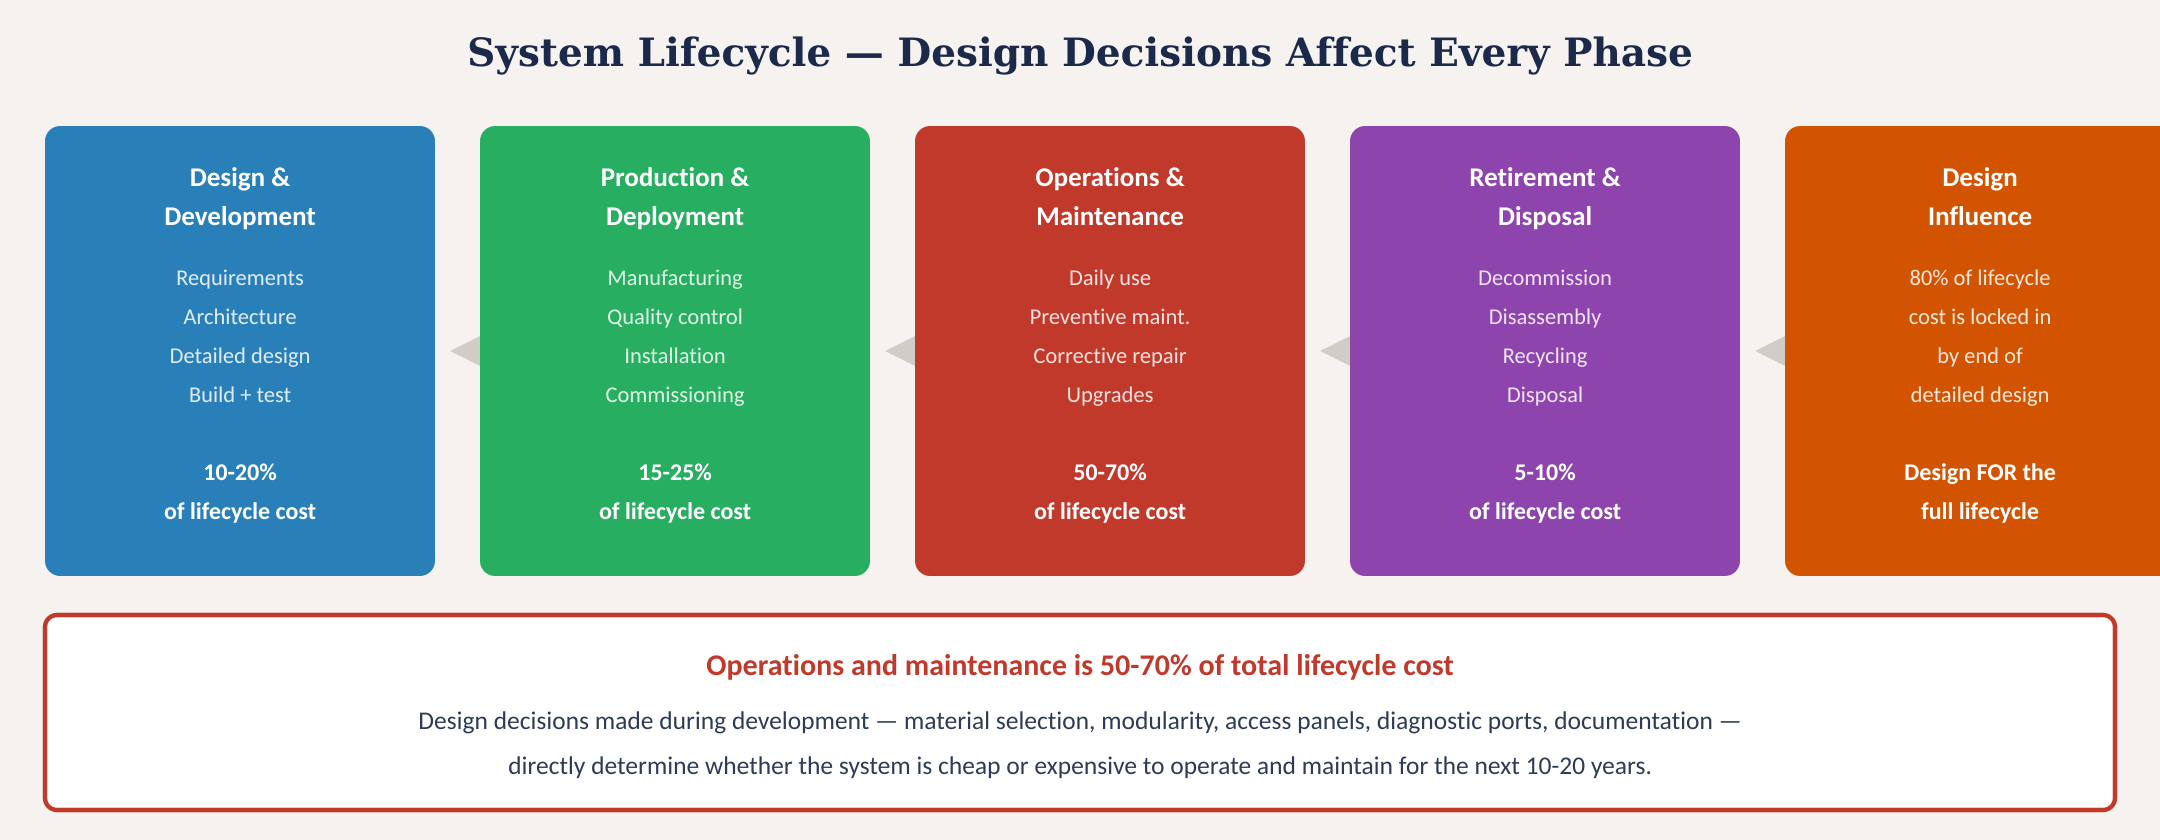
\includegraphics[width=\textwidth]{master_figs/fig_system_lifecycle.png}
\caption{System lifecycle with cost distribution.}\end{figure}

\begin{figure}[htbp]\centering
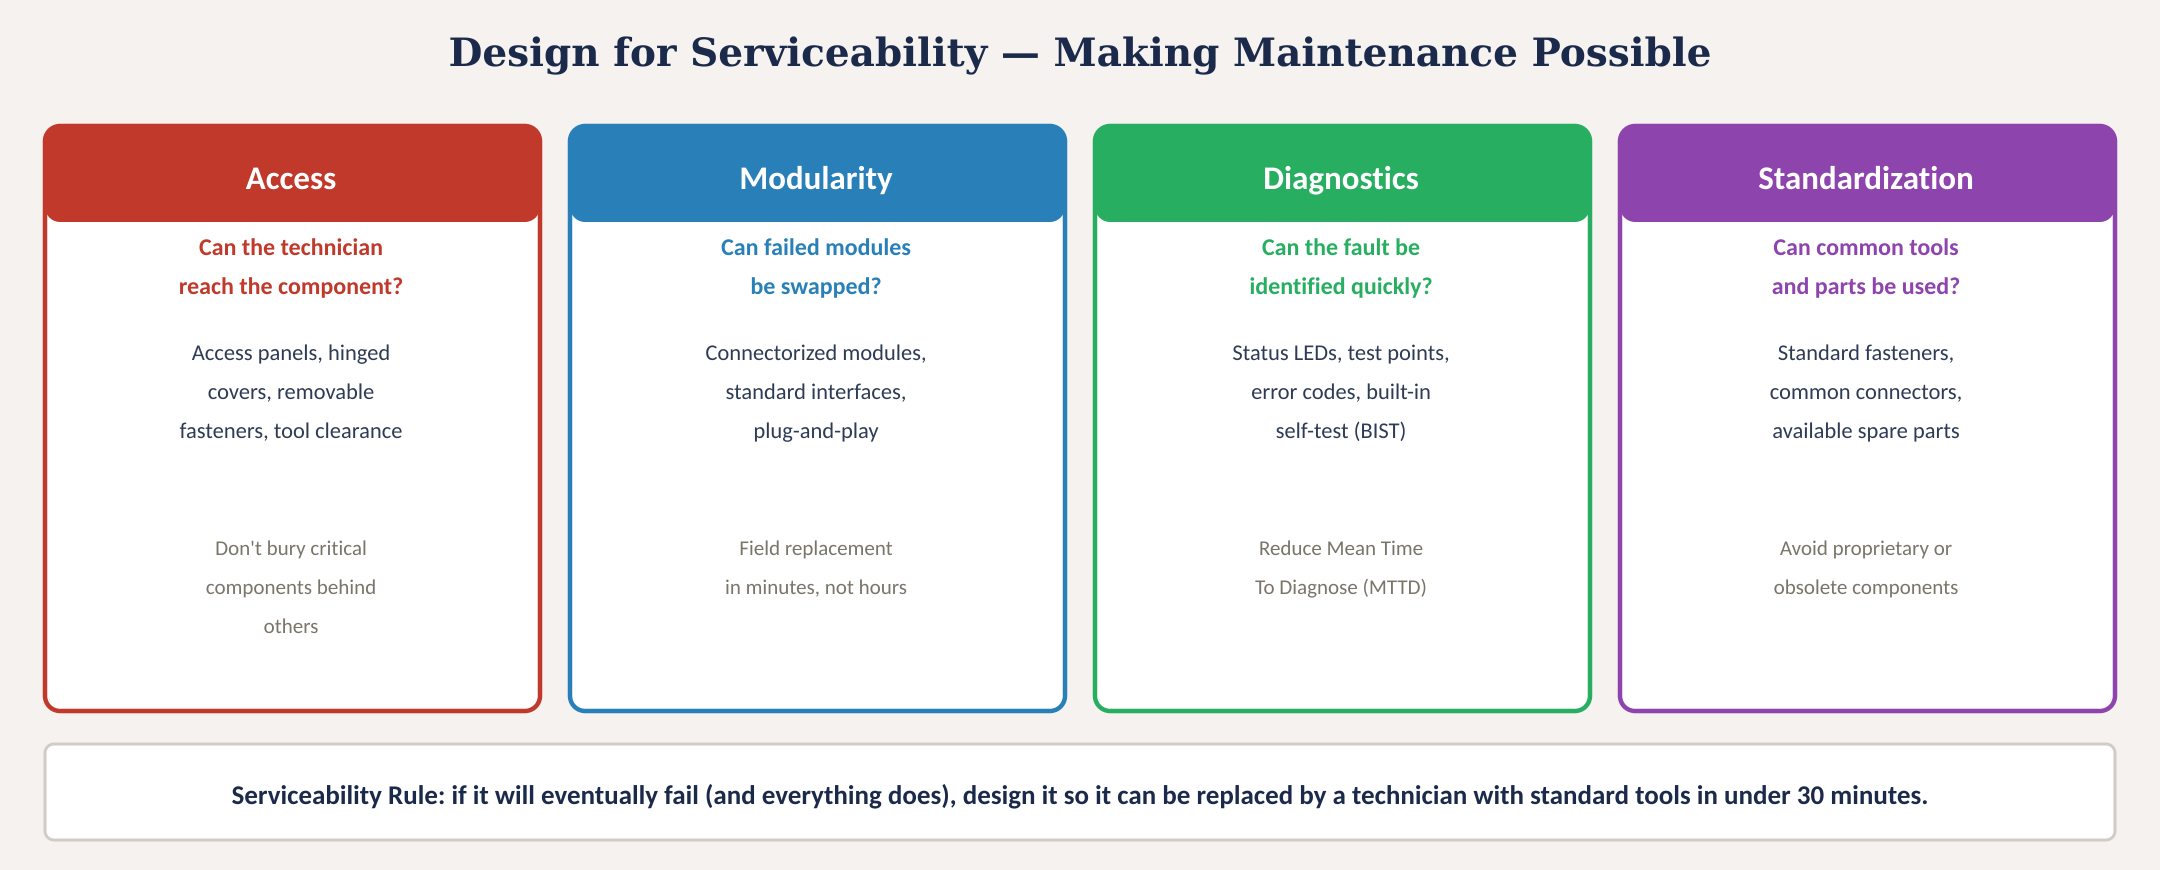
\includegraphics[width=\textwidth]{master_figs/fig_serviceability.png}
\caption{Four serviceability principles.}\end{figure}

\begin{figure}[htbp]\centering
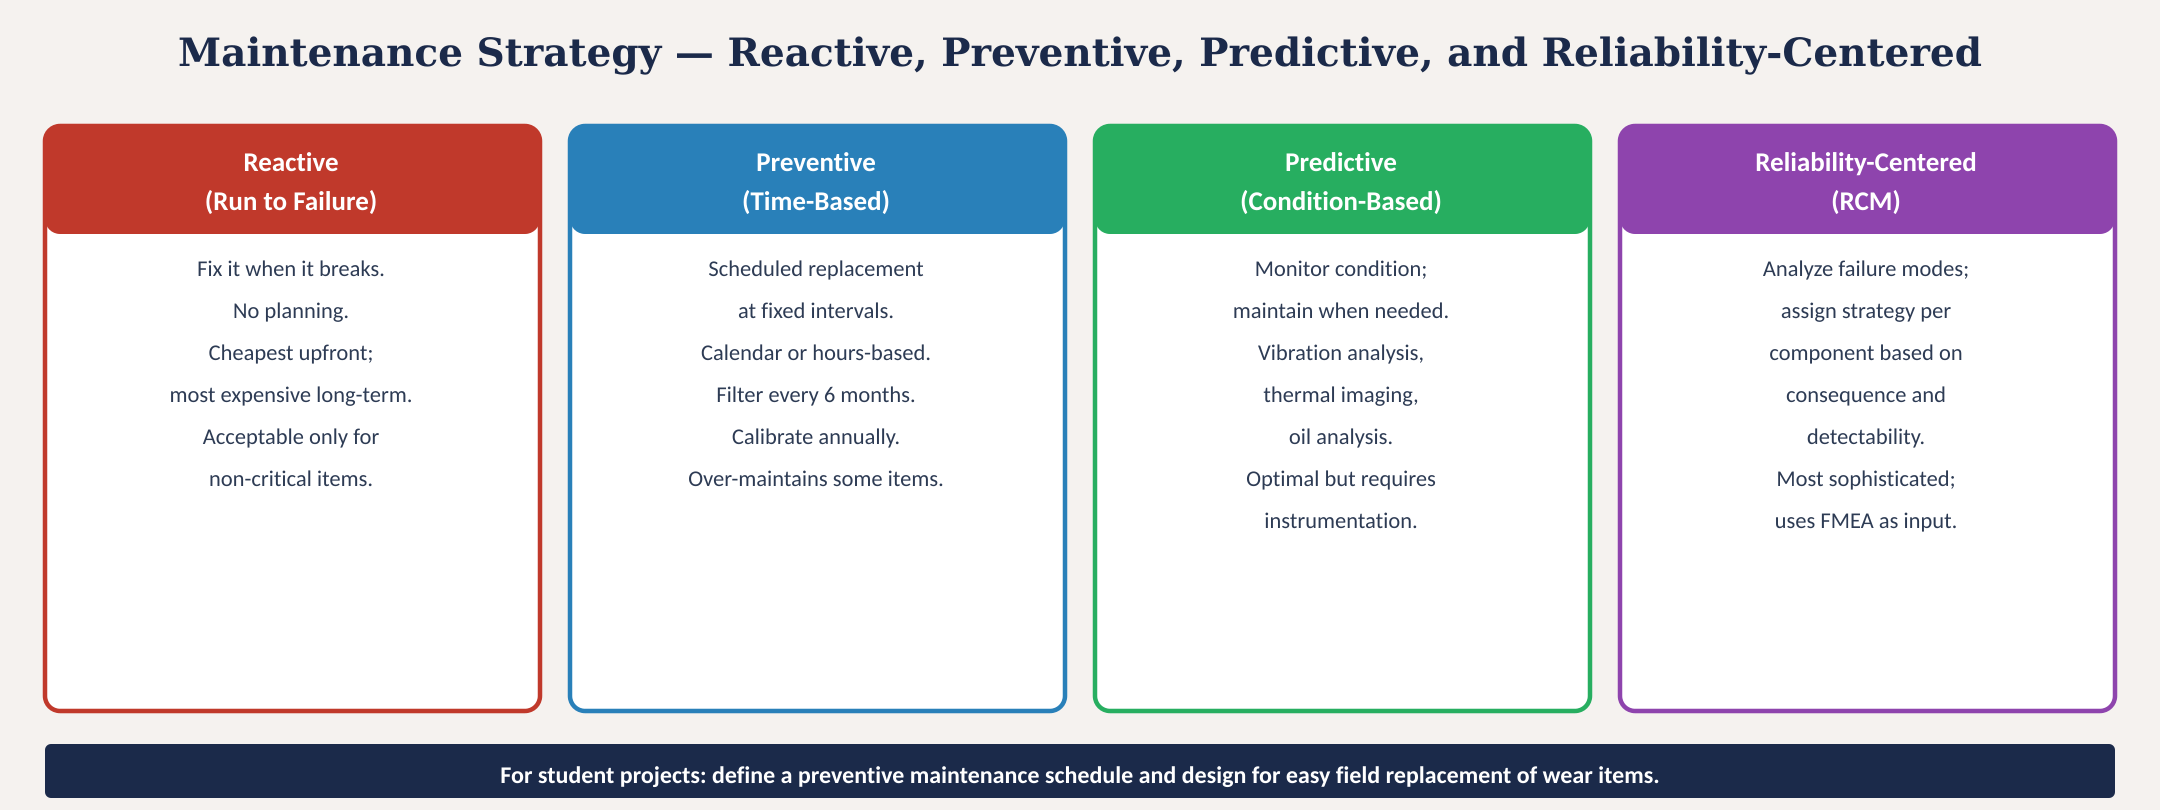
\includegraphics[width=\textwidth]{master_figs/fig_maintenance_strategies.png}
\caption{Maintenance strategies from reactive to RCM.}\end{figure}

\begin{figure}[htbp]\centering
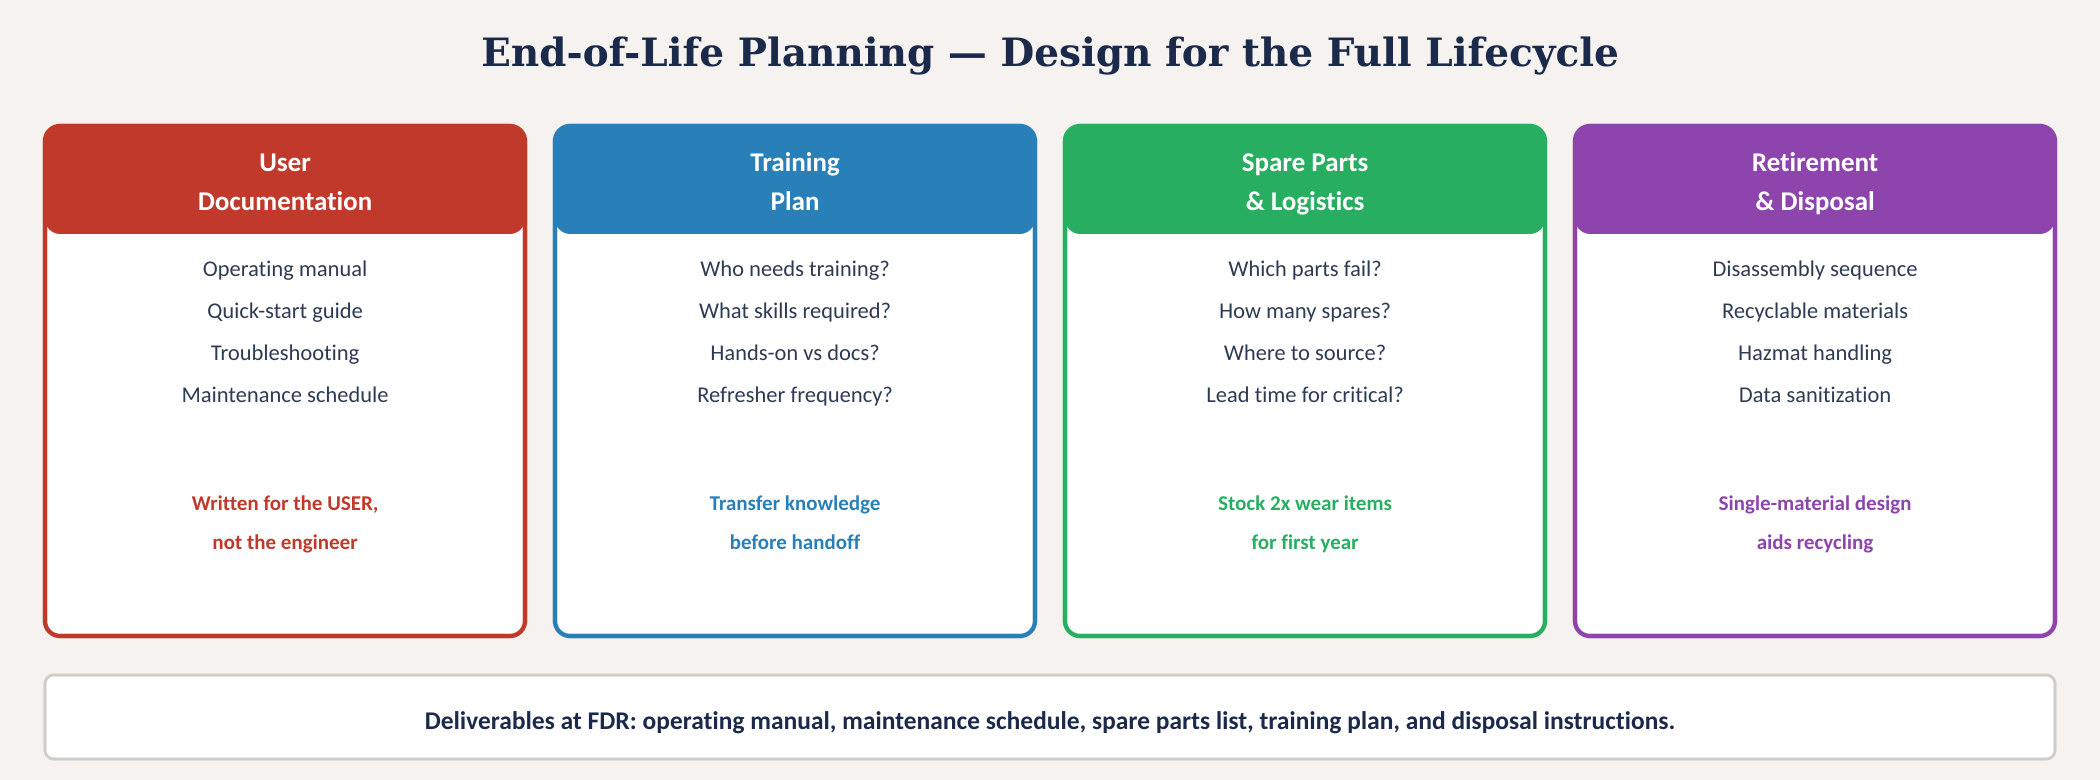
\includegraphics[width=\textwidth]{master_figs/fig_eol_planning.png}
\caption{End-of-life planning deliverables.}\end{figure}

\section{Lifecycle Thinking}
Operations and maintenance accounts for 50--70\% of total lifecycle cost — far more than development. 80\% of that cost is locked in by decisions made during concept and preliminary design. This means design-for-serviceability, maintainability, and disposability must be considered DURING design.

\section{Design for Serviceability}
Four principles: \textbf{Access} (can the technician reach the component? Use access panels, hinged covers, quick-release fasteners), \textbf{Modularity} (can failed modules be swapped? Connectorized, independently testable), \textbf{Diagnostics} (can the fault be identified? Status LEDs, test points, error codes, BIST), \textbf{Standardization} (can common tools and parts be used? Standard fasteners, multi-source components).

\subsection{Reliability Metrics}
MTBF (Mean Time Between Failures) and MTTR (Mean Time To Repair) combine to give Availability:
\[
A = \frac{\text{MTBF}}{\text{MTBF} + \text{MTTR}}
\]
Improving MTTR through better serviceability design is often cheaper than improving MTBF through better components. FMEA identifies failure modes and prioritizes design improvements.


\subsection{The Bathtub Curve}
Component failure rate follows three phases: (1)~\textbf{Infant mortality} (decreasing rate): manufacturing defects fail early. Mitigate with burn-in testing. (2)~\textbf{Useful life} (constant rate): random failures at steady rate; the MTBF region. (3)~\textbf{Wear-out} (increasing rate): fatigue, corrosion, seal degradation. Mitigate with preventive replacement.

For student projects, most failures occur in Phase~1 (build quality). Burn in your system for 48+ hours before final demo.

\subsection{FMECA: Failure Modes, Effects, and Criticality Analysis}
FMECA extends FMEA by adding \textbf{Criticality Analysis}. For MEGN~301, use simplified FMEA with RPN (Risk Priority Number = Severity $\times$ Occurrence $\times$ Detection, each 1--10). Focus design effort on top-5 RPN items.

\subsection{Writing Maintainability Requirements}
Examples of maintainability requirements:
\begin{itemize}[nosep,leftmargin=1.5em]
\item ``The system shall allow sensor replacement without disassembling the enclosure.''
\item ``The system shall provide visual indication (LED) of power, communication, and fault status.''
\item ``The system shall allow firmware update via USB without opening the enclosure.''
\item ``All field-replaceable modules shall use tool-free connectors (no soldering).''
\end{itemize}

\begin{greenshieldbox}[GreenShield: O\&M Requirement Trace]
\small
\begin{tabularx}{\textwidth}{l X l}
\toprule
\textbf{Req ID} & \textbf{O\&M Requirement} & \textbf{Parent Need} \\
\midrule
OM-001 & Sensor replacement w/o enclosure disassembly & Operator cannot solder \\
OM-002 & Status LEDs for power, comms, fault & Remote monitoring need \\
OM-003 & Battery replacement $<$5 min & Off-grid solar concept \\
\bottomrule
\end{tabularx}
\end{greenshieldbox}

\begin{keyconceptbox}[Industry SE Parallels]
\begin{itemize}[nosep,leftmargin=1.5em]
\item \textbf{INCOSE SEH 4th ed.}: \S4.12--4.15 (Transition, Operation, Maintenance, Disposal).
\item \textbf{NASA SP-2016-6105 Rev~2}: Ch.~6.3 Reliability, Maintainability, and Availability.
\item \textbf{MIL-STD-1629A}: FMECA procedures.
\end{itemize}
\end{keyconceptbox}

\section{Artifact Handoff: What Chapter 6 Produces}
\begin{table}[htbp]\centering\small
\begin{tabularx}{\textwidth}{l X l}
\toprule
\textbf{Artifact} & \textbf{Description} & \textbf{Used In} \\
\midrule
O\&M Manual & Quick-start, operating, maintenance, troubleshooting guides & FDR \\
FMEA/FMECA & Failure mode analysis with RPN ranking & Design iteration \\
Spare Parts List & Wear items with vendors and intervals & Handoff package \\
\bottomrule
\end{tabularx}
\end{table}

\section{Maintenance Planning}
Four strategies: \textbf{Reactive} (run to failure — cheapest upfront, most expensive long-term), \textbf{Preventive} (scheduled replacement at fixed intervals), \textbf{Predictive} (condition-based monitoring), \textbf{Reliability-Centered} (FMEA-driven strategy per component). For student projects: define a preventive schedule and design for easy field replacement.

Build a maintenance schedule: identify wear items, define replacement intervals, create a spare parts list with vendors and lead times, and establish a calibration schedule.

\section{Documentation, Training, and End-of-Life}
Four documentation types: Quick-Start Guide (1 page, 10-minute setup), Operating Manual (complete reference by task), Maintenance Manual (step-by-step procedures with photos), Troubleshooting Guide (symptom-based flowcharts).

Training plan: identify audiences (operators, maintainers, trainers), methods (hands-on, written, video), and competency assessment. Knowledge transfer: document design rationale, known limitations, and workarounds.


\subsection{Design for Disassembly (DfD)}
Sustainability begins with designing systems that can be taken apart. Write this as a formal requirement:

\begin{quote}
\textbf{DfD-REQ-001}: The system shall be fully disassembled into its base material categories (metal, polymer, electronics, hazardous) using only standard hand tools (Phillips screwdriver, hex key set, pliers) in $\leq$5 minutes by a single technician.
\end{quote}

This is a \textbf{testable requirement}; verify it by demonstration (TAID method ``D'') at FDR. Time the disassembly; if it exceeds 5 minutes, the design fails the requirement. Practical rules: use fasteners instead of adhesives, avoid mixed-material bonding (epoxy on sensors is fast but makes recycling impossible), label material type on each component or enclosure panel, and design snap-fits to be releasable (not permanently locked).

End-of-life: design for disassembly (fasteners not adhesives), single-material design for recyclability, hazardous material handling (batteries, solvents), data sanitization.


\subsection{The Bathtub Curve}
Component failure rate follows the ``bathtub curve'':
\begin{enumerate}[nosep,leftmargin=1.5em]
\item \textbf{Infant mortality} (decreasing rate): manufacturing defects and weak components fail early. Mitigate with burn-in testing and quality inspection.
\item \textbf{Useful life} (constant rate): random failures at a steady rate. This is the MTBF region.
\item \textbf{Wear-out} (increasing rate): fatigue, corrosion, seal degradation, bearing wear. Mitigate with preventive replacement before onset.
\end{enumerate}
For student projects, most failures occur in Phase~1 (build quality). Burn-in your system for 48+ hours before the final demonstration.

\subsection{FMECA: Failure Modes, Effects, and Criticality Analysis}
\textbf{Important}: Your FMEA should have \emph{started} during concept generation and architecture (Chapters~2--3), not here. By the O\&M phase, you are updating the FMEA with field-observed failure data and refining RPN scores, not creating it from scratch. If your team's first FMEA appears at FDR, it is too late to design out any failure mode it reveals.

FMECA extends FMEA by adding \textbf{Criticality Analysis}. For MEGN~301, use simplified FMEA with RPN (Risk Priority Number = Severity $\times$ Occurrence $\times$ Detection, each 1--10). Focus design effort on the top 5 RPN items.

\subsection{Writing Maintainability Requirements}
Examples of often-neglected maintainability requirements:
\begin{itemize}[nosep,leftmargin=1.5em]
\item ``The system shall allow sensor replacement without disassembling the enclosure.''
\item ``The system shall provide LED indication of power, communication, and fault status.''
\item ``The system shall allow firmware update via USB without opening the enclosure.''
\item ``All field-replaceable modules shall use tool-free connectors.''
\end{itemize}

\begin{greenshieldbox}[GreenShield: O\&M Requirement Trace]
\small
\begin{tabularx}{\textwidth}{l X l}
\toprule
\textbf{Req ID} & \textbf{O\&M Requirement} & \textbf{Parent Need} \\
\midrule
OM-001 & Sensor replacement without enclosure disassembly & Operator cannot solder \\
OM-002 & Status LEDs for power, comms, fault & Remote monitoring \\
OM-003 & Battery replacement $<$5 min & Off-grid concept \\
OM-004 & All wear items documented with intervals & Long-term operation \\
\bottomrule
\end{tabularx}
\end{greenshieldbox}

\begin{keyconceptbox}[Industry SE Parallels]
\begin{itemize}[nosep,leftmargin=1.5em]
\item \textbf{INCOSE SEH 4th ed.}: Sec.\ 4.12--4.15 (Transition, Operation, Maintenance, Disposal).
\item \textbf{NASA SP-2016-6105 Rev 2}: Ch.\ 6.3 (Reliability, Maintainability, Availability).
\item \textbf{IEC 60300}: Dependability management standards.
\item \textbf{MIL-STD-1629A}: Procedures for performing FMECA.
\end{itemize}
\end{keyconceptbox}

\section{Artifact Handoff: What Chapter 6 Produces}
\begin{table}[htbp]\centering\small
\begin{tabularx}{\textwidth}{l X l}
\toprule
\textbf{Artifact} & \textbf{Description} & \textbf{Forward Reference} \\
\midrule
O\&M Manual & Quick-start, operating, maintenance, troubleshooting guides & FDR deliverable \\
FMEA/FMECA & Failure mode analysis with RPN ranking & Design iteration \\
Spare Parts List & Wear items with vendors, lead times, replacement intervals & Handoff package \\
\bottomrule
\end{tabularx}
\end{table}

\section{Operational Concepts}
Every engineered system has an operational context: who uses it, where, how often, for how long, and under what conditions. The operational concept document (ConOps) describes this context and drives design decisions for reliability, maintainability, and user interface.

\textbf{Duty cycle}: how much of the time is the system operating? A continuously running process monitor (100\% duty cycle) has very different reliability requirements than a laboratory instrument used 2 hours per week (1.2\% duty cycle). High duty cycles demand higher-reliability components and shorter maintenance intervals.

\textbf{Operating environment}: indoor laboratory (controlled temperature, clean, stable power) vs.\ outdoor field installation (temperature extremes, moisture, vibration, unreliable power) vs.\ vehicle-mounted (high vibration, temperature cycling, EMI from engine). The environment determines the required IP rating, vibration qualification, temperature range, and EMC compliance.

\textbf{Operator skill level}: a research instrument operated by a PhD engineer can tolerate a complex interface and manual calibration procedures. A production tool operated by a technician must be intuitive with minimal training. A consumer product must be operable by anyone with no training. Design the interface for the least skilled expected operator.

\section{Reliability Engineering Basics}
\textbf{Mean Time Between Failures (MTBF)}: the average time a system operates before a failure occurs. For electronic systems, MTBF is predicted from component failure rates using MIL-HDBK-217 or the FIDES methodology. The system MTBF is approximately the reciprocal of the sum of all component failure rates: $\text{MTBF}_{\text{system}} \approx 1/\sum \lambda_i$.

\textbf{Reliability}: the probability that the system operates without failure for a specified time. For exponentially distributed failures: $R(t) = e^{-t/\text{MTBF}}$. For a system with MTBF $= 10{,}000$ hours, the probability of surviving 1000 hours without failure is $R = e^{-1000/10000} = 0.905$ (90.5\%).

\textbf{Availability}: the fraction of time the system is operational: $A = \text{MTBF}/(\text{MTBF} + \text{MTTR})$ where MTTR is the Mean Time To Repair. A system with MTBF $= 10{,}000$ hours and MTTR $= 2$ hours has availability $= 99.98\%$.

\section{Maintainability Design Principles}
\textbf{Accessibility}: components that require periodic maintenance (filters, batteries, calibration adjustments) must be accessible without disassembling the entire system. Place maintenance items on the exterior or behind easily removed panels.

\textbf{Standardized fasteners}: use the minimum number of fastener types. Ideally, the entire system can be serviced with one screwdriver size. Avoid exotic fastener types (Torx, tri-wing, pentalobe) unless security is a requirement.

\textbf{Modular replacement}: design subsystems as Line Replaceable Units (LRUs) that can be swapped in the field without specialized tools or calibration. A failed sensor module should be replaceable by unplugging a connector, removing two screws, and plugging in a new module. Total repair time target: $< 15$ minutes for any single-point failure.

\textbf{Diagnostic capability}: include built-in self-test (BIST) features that identify the failed subsystem. An LED that blinks a fault code, a serial output that reports sensor status, or a display that shows system health enables rapid diagnosis. Without diagnostics, troubleshooting is trial-and-error, which is slow and risks introducing new problems.

\textbf{Spare parts strategy}: identify the components most likely to fail (wear parts, connectors, fuses) and stock spares. For MEGN~301 projects, include a ``recommended spares'' list in the maintenance manual.

\section{User Documentation}
A delivered system requires three documents:

\textbf{User manual}: how to operate the system. Step-by-step instructions for startup, normal operation, shutdown, and common adjustments. Written for the end user (non-engineer). Include photographs, not just text.

\textbf{Maintenance manual}: how to maintain and repair the system. Scheduled maintenance procedures (cleaning, calibration, consumable replacement). Troubleshooting guide (symptom $\to$ probable cause $\to$ corrective action). Exploded assembly diagrams showing part numbers and locations.

\textbf{Technical reference}: for the engineer who will eventually modify or upgrade the system. Complete schematics, firmware source code, mechanical drawings, BOM, calibration data, and design rationale. This is essentially the FDR package, archived for future reference.

\section{Preventive Maintenance Scheduling}
Based on component life data and operating conditions, create a maintenance schedule:

\begin{itemize}[nosep,leftmargin=1.5em]
\item \textbf{Daily}: visual inspection, check indicator lights, verify normal operation.
\item \textbf{Weekly}: clean sensors and optical surfaces, check fluid levels, verify calibration against reference.
\item \textbf{Monthly}: inspect wiring and connectors for damage, exercise manual overrides, backup data and firmware.
\item \textbf{Annually}: replace batteries, recalibrate all sensors against traceable standards, inspect mechanical wear items (bearings, seals, belts), update firmware to latest version.
\end{itemize}
\section{Failure Analysis and Root Cause Investigation}
When a system fails in operation, a structured failure analysis prevents recurrence:

\textbf{Preserve the evidence}: do not immediately ``fix'' the failure. Photograph the system in its failed state. Record sensor logs, error messages, and environmental conditions at the time of failure. If a component physically failed (burned resistor, cracked solder joint, stripped gear), save the failed part for examination.

\textbf{Fault tree analysis}: work backward from the failure event to identify all possible causes. Draw a tree diagram with the top event (system failure) and branch into causes and sub-causes. For ``motor stopped running'': branches include power supply failure (fuse blown, wire disconnected), motor failure (winding open, bearing seized), driver failure (MOSFET destroyed, control signal absent), and software failure (watchdog reset, state machine stuck).

\textbf{5 Whys}: for each branch of the fault tree, ask ``why?'' repeatedly until the root cause is identified. ``Motor stopped'' $\to$ why? ``Bearing seized'' $\to$ why? ``Lubrication depleted'' $\to$ why? ``No lubrication schedule in maintenance plan'' $\to$ root cause: inadequate maintenance documentation. The corrective action addresses the root cause (add lubrication to the maintenance schedule), not just the symptom (replace the bearing).

\section{Warranty and Service Planning}
For products intended for deployment beyond the classroom:

\textbf{Warranty period}: how long does the manufacturer (your team) guarantee the product will work? Industry standard for electronic products: 1--3 years. During the warranty period, the manufacturer repairs or replaces the product at no cost.

\textbf{Service model}: who performs maintenance and repair? Three models:

(1) \emph{Return to manufacturer}: the user sends the product back for repair. Longest downtime but ensures repairs are done correctly. Appropriate for complex, high-value products.

(2) \emph{Field service}: a trained technician visits the user's site. Fastest repair but most expensive per incident. Appropriate for critical equipment that cannot be offline.

(3) \emph{User-serviceable}: the user performs routine maintenance and simple repairs using the maintenance manual. Lowest cost but requires adequate documentation and training. The GreenShield model: design for user serviceability with a clear maintenance manual.

\section{Technical Data Package}
At the end of the project, the team delivers a complete Technical Data Package (TDP) that enables anyone to reproduce, maintain, modify, and eventually retire the system:

\begin{itemize}[nosep,leftmargin=1.5em]
\item System Design Requirements Document (SDRD), final revision
\item Mechanical drawings (CAD files, 2D drawings, assembly instructions)
\item Electrical schematics and PCB layout files
\item Bill of Materials with supplier links and current pricing
\item Firmware source code with build instructions and version history
\item Calibration procedure and data
\item Test plan, test procedures, and test results (VCRM)
\item User manual
\item Maintenance manual with spare parts list
\item Disassembly and disposal procedure (Chapter~9)
\item Design rationale document (key decisions with justification)
\end{itemize}

The TDP is the team's professional legacy. A complete TDP demonstrates engineering maturity; an incomplete one demonstrates technical debt.

\section{Obsolescence Management}
Electronic components have shorter market lifetimes than the products they go into. An IC available today may be discontinued in 3--5 years. Strategies:

\textbf{Design with widely used, multi-sourced components}: the ESP32 has millions of units in production; it will be available for years. An obscure sensor from a single manufacturer may be discontinued without notice.

\textbf{Document alternatives}: for each critical component, identify at least one alternative that could be substituted with minor redesign. Record these in the BOM notes.

\textbf{Lifetime buy}: if a critical component is announced for end-of-life (EOL), purchase enough stock for the expected remaining production run. This is a common industrial practice but rarely relevant for MEGN~301 projects.

\textbf{Modular design}: isolating the component-specific interface in a replaceable module means that when a component becomes obsolete, only the module needs redesign, not the entire system.
\section{Practice Questions}
\begin{enumerate}[leftmargin=1.5em]
\item A system has MTBF = 2000 hrs and MTTR = 24 hrs. Calculate availability. Propose two design changes to improve availability, one targeting MTBF and one targeting MTTR.
\item Write a quick-start guide (1 page, numbered steps) for a greenhouse temperature monitoring system.
\item Your project sponsor asks why you budgeted \$200 for spare parts on a \$2000 project. Justify the expenditure.
\item Identify all wear items in an electromechanical system with a DC motor, belt drive, pressure sensor, and lithium battery. Define replacement intervals for each.
\item Sketch the bathtub curve and label all three regions. Your system fails twice in the first week then runs flawlessly for 6 months. What region were the initial failures in, and how should you have prevented them?
\item Write a simplified FMEA (Severity/Occurrence/Detection, 1--10 each) for a greenhouse frost protection system with at least 5 failure modes. Calculate RPN for each.
\item Your sponsor asks why you need an O\&M manual for a one-semester student project. Argue why it is still necessary.
\end{enumerate}

\subsection{Answers}
\begin{enumerate}[leftmargin=1.5em]
\item Availability = MTBF/(MTBF+MTTR) = 2000/(2000+24) = 98.8\%. Improving MTBF: use industrial-grade components with higher rated life; add redundancy (dual sensors). Improving MTTR: add diagnostic LEDs and test points for faster fault isolation; use modular, connectorized design so a failed module can be swapped in $<$5 minutes instead of 24 hours.
\item Quick-start guide: (1) Unbox system. (2) Mount sensor probe inside greenhouse at plant height using provided bracket. (3) Connect sensor cable to controller box (keyed connector). (4) Plug wall adapter into 120\,VAC outlet. (5) Verify green POWER LED is on. (6) Set temperature threshold using the dial on the front panel (default: 3\,\degC{}). (7) Verify amber MONITORING LED blinks once per second. (8) Test: hold ice cube near sensor. Within 30\,s, red HEATER LED should illuminate. Setup complete.
\item The \$200 spare parts budget is insurance against project failure. Motors wear out, sensors break, PCBs develop faults during testing, and connectors get damaged during repeated assembly/disassembly. Without spares, a single component failure can halt the project for 1--3 weeks (ordering + shipping). At \$200/\$2000 = 10\% of project cost, this is standard engineering practice. Industry typically budgets 5--15\% of project cost for spares and consumables.
\item Wear items: DC motor brushes (replace at 2000--5000 hrs), belt (inspect at 500 hrs, replace at 1000 hrs or on visible cracking), pressure sensor diaphragm (inspect annually, replace at first sign of drift), lithium battery (capacity degrades; replace when capacity $<$80\% of rated, typically 300--500 charge cycles). Additionally: all O-rings and seals in fluid connections (annual replacement), and any connectors subject to repeated mating cycles.
\item Bathtub curve: decreasing (infant mortality), constant (useful life), increasing (wear-out). Two failures in week one = infant mortality phase. Prevention: (a) burn-in test for 48+ hours before deployment, (b) inspect all solder joints and connections during assembly, (c) verify all power rails under load before system-level testing. The flawless 6-month period = useful life phase with constant (low) failure rate.
\item FMEA example (abbreviated): Sensor reads high (S=8, O=3, D=4, RPN=96), Relay stuck closed (S=9, O=2, D=6, RPN=108), MCU brown-out (S=7, O=4, D=5, RPN=140), GSM no signal (S=5, O=3, D=3, RPN=45), Power supply fails open (S=8, O=2, D=7, RPN=112). Action priority: MCU brown-out first (decoupling + supervisor), then power supply (add status LED + fuse), then relay (add thermal fuse), then sensor (add second sensor for comparison).
\item The O\&M manual is necessary because: (a) it is a primary FDR deliverable, the project is not complete without it; (b) the instructor and future teams need to operate, maintain, and build upon your work; (c) writing the manual forces you to think about failure modes, maintenance procedures, and spare parts, improving the design; (d) in industry, a product without O\&M documentation is undeliverable.
\end{enumerate}



% ================================================================
\chapter{Post-Build Testing, Verification \& Validation}

\section{Why Testing Is a Separate Engineering Activity}
Building the system is not the end of the engineering process; it is the beginning of a critical phase that determines whether the system actually works. Testing reveals the gap between what you designed and what you built. Verification asks: ``did we build the product right?'' (does it meet its specifications). Validation asks: ``did we build the right product?'' (does it satisfy the user's actual needs). Both must be answered affirmatively before the system is ready for deployment.

In MEGN~301, this chapter addresses what happens after your GreenShield prototype is assembled and powered on for the first time. The activities described here occur between subsystem integration (Chapter~5) and the Final Design Review (FDR), and they produce the evidence that the FDR review board needs to assess your project's success.

\section{Test Planning and Documentation}
\subsection{The Test Plan}
A test plan is a document that specifies what will be tested, how, by whom, with what equipment, and what constitutes pass/fail. It should be written during the design phase (Chapter~4) and refined during integration. Key elements:

\textbf{Test ID}: unique identifier (e.g., TVR-007 for Test/Verification/Requirement 007).

\textbf{Requirement traced}: the specific ``shall'' statement being verified (from the SDRD).

\textbf{Test method}: one of four categories from systems engineering: Test (T), Analysis (A), Inspection (I), or Demonstration (D).

\textbf{Test procedure}: step-by-step instructions that another engineer could follow to reproduce the test. Include setup, equipment list, input conditions, measurement points, and acceptance criteria.

\textbf{Pass/fail criteria}: quantitative thresholds derived directly from the requirement. ``The motor shall produce at least 0.5\,N$\cdot$m of torque at 500\,RPM'' becomes ``PASS if measured torque $\geq 0.5$\,N$\cdot$m at $500 \pm 10$\,RPM; FAIL otherwise.''

\textbf{Test data record}: a template for recording the raw data, environmental conditions, equipment serial numbers, and tester's name. This is the evidence file for the FDR.

\subsection{Verification Cross-Reference Matrix (VCRM)}
The VCRM is a table that maps every requirement in the SDRD to its corresponding test. It answers: ``for each requirement, how do we know it is met?'' A gap in the VCRM (a requirement with no corresponding test) means that requirement is unverified; it could be met or not, and nobody knows. An incomplete VCRM is one of the most common deficiencies found at FDR.

\begin{greenshieldbox}[GreenShield Template: VCRM Format]
\begin{tabularx}{\textwidth}{l l l l l}
\toprule
\textbf{Req ID} & \textbf{Requirement} & \textbf{Method} & \textbf{Test ID} & \textbf{Status} \\
\midrule
SYS-001 & Shall operate on 12\,V DC & T & TVR-001 & PASS \\
SYS-002 & Shall weigh $<$2\,kg & I & TVR-002 & PASS \\
SYS-003 & Shall maintain 50$\pm$1\,\degC{} & T & TVR-003 & FAIL (see NCR-01) \\
\bottomrule
\end{tabularx}
Any FAIL result must be documented in a Non-Conformance Report (NCR) with root cause analysis and corrective action plan.
\end{greenshieldbox}

\section{Functional Testing}
Functional testing verifies that each function specified in the requirements is operational. It is the most basic level of testing: does the system do what it is supposed to do?

\textbf{Power-on self-test (POST)}: verify the system initializes correctly. Check: power LED illuminates, MCU boots (serial output or indicator), all sensors report plausible values (not NaN, not railed), all actuators respond to a brief test command (motor spins for 0.5\,s, LED blinks, valve clicks). The POST should be the first thing you run after integration, and it should be automated in firmware.

\textbf{Input-output verification}: for each sensor, apply a known input and verify the output is within the calibrated range. For each actuator, command a known output and verify the physical response. This confirms that the wiring, signal conditioning, firmware, and calibration are all correct.

\textbf{Nominal operation test}: run the system through its normal operating sequence (the ``happy path''). For a temperature controller: set the target, wait for the system to reach setpoint, verify stability, change the setpoint, verify the transition. Document the results with time-stamped data and photographs.

\section{Performance Testing}
Performance testing measures how well the system performs its functions. It goes beyond ``does it work?'' to ``how well does it work?''

\textbf{Accuracy testing}: compare the system's output to a calibrated reference across the operating range. For a temperature controller: measure the actual temperature with a calibrated reference thermometer at 5--10 setpoints spanning the range. Plot the error (system reading minus reference) vs.\ setpoint. The maximum error must be within the accuracy specification.

\textbf{Repeatability testing}: repeat the same measurement or operation 10--20 times under identical conditions. Compute the standard deviation. The repeatability must be within the specification. If the system meets the accuracy spec on average but has high scatter (poor repeatability), it is unreliable even if individual tests happen to pass.

\textbf{Response time testing}: measure the time from a step input (setpoint change, disturbance) to the output reaching the specified percentage of its final value (typically 90\% or 95\%). Compare to the response time specification. For control systems: measure rise time, settling time, and overshoot from the step response data.

\textbf{Boundary and stress testing}: operate the system at the extremes of its specified range. Test at the maximum and minimum input, the maximum and minimum power supply voltage ($\pm$10\% typical), the maximum and minimum ambient temperature, and the maximum load. Verify that the system still meets all specifications at these extremes. Systems that pass nominal testing but fail at boundaries have insufficient design margin.

\section{Environmental and Robustness Testing}
\textbf{Vibration and shock}: for portable or vehicle-mounted systems, shake or drop the system and verify continued operation. Even a brief vibration test (hand-shake the enclosure while monitoring sensor outputs) reveals loose connections, poorly secured components, and resonant structural elements.

\textbf{Thermal cycling}: if the system will operate in varying temperatures, cycle it between the temperature extremes 5--10 times and verify operation at each extreme. Thermal cycling stresses solder joints, connector contacts, and adhesive bonds.

\textbf{EMI susceptibility}: operate the system near a running motor, a switching power supply, or a cell phone transmitting. Monitor sensor outputs for noise, glitches, or erroneous readings. If the system is sensitive to EMI, improve shielding and grounding before deployment.

\textbf{Water and dust exposure}: if the system will operate outdoors or in industrial environments, test resistance to splash (IP rating). Even a brief spray test reveals unsealed enclosure joints, exposed connectors, and inadequate conformal coating.

\section{Validation: Does It Solve the Problem?}
Verification confirms the system meets its specifications. Validation confirms the specifications themselves are correct: that meeting them actually solves the user's problem. Validation is harder because it requires engagement with real users in realistic conditions.

\textbf{User acceptance testing (UAT)}: give the system to a representative user (not a team member) and observe them operating it. Note: where they hesitate, what they do wrong, what they find confusing, and whether the outcome meets their expectations. The user's experience often reveals requirements that were missed or misinterpreted.

\textbf{Field trial}: operate the system in its intended environment for an extended period (days to weeks). Monitor for degradation, unexpected failure modes, environmental effects, and user feedback. The field trial often reveals issues that laboratory testing cannot: intermittent failures, long-term drift, user workflow conflicts, and environmental exposures not anticipated in the test plan.

\textbf{Stakeholder review}: present the test results to all stakeholders (user, sponsor, advisor, safety officer) and obtain explicit acceptance. The FDR serves this function in MEGN~301.

\section{Non-Conformance and Corrective Action}
When a test fails, the response follows a structured process:

(1) \textbf{Document the failure}: what was tested, what was expected, what was observed, and what the deviation is. This is the Non-Conformance Report (NCR).

(2) \textbf{Root cause analysis}: why did it fail? Use the ``5 Whys'' technique: ask ``why'' iteratively until the root cause (not just the symptom) is identified. ``The motor stalled'' $\to$ why? ``Insufficient torque'' $\to$ why? ``Current limited by the MOSFET driver'' $\to$ why? ``Gate voltage only 3.3\,V, MOSFET needs 5\,V for full enhancement'' $\to$ root cause: wrong MOSFET selected for 3.3\,V logic.

(3) \textbf{Corrective action}: fix the root cause, not just the symptom. Replace the MOSFET with a logic-level type, not just increase the motor voltage.

(4) \textbf{Retest}: after the corrective action, retest the specific requirement that failed. Also retest any related requirements that could have been affected by the change (regression testing).

(5) \textbf{Close the NCR}: document the corrective action taken, the retest results, and the final disposition (PASS after rework, or Accept-as-is with justification, or Reject/Redesign).

\section{Test Report and FDR Evidence Package}
The test report is the primary evidence document for the FDR. It should include:

\begin{itemize}[nosep,leftmargin=1.5em]
\item Test plan (what was supposed to be tested)
\item VCRM with status of each requirement (PASS/FAIL/UNTESTED)
\item Raw test data with timestamps, equipment used, and environmental conditions
\item Photographs and videos of key tests
\item Analysis of any failed tests (NCRs with root cause and corrective action)
\item Summary statistics (number of requirements, number verified, number of failures, number of open NCRs)
\item Conclusion: overall system readiness assessment
\end{itemize}

\begin{warningbox}[Test What You Ship, Ship What You Test]
The system presented at FDR must be the same system that was tested. Any modification made after testing (even a ``minor'' firmware update or a ``quick'' wiring fix) invalidates the test results for any requirement that could be affected by the change. If you make changes after testing, retest the affected requirements and update the test report.
\end{warningbox}

\section{Test Equipment for MEGN 301}
The following equipment is available in the MEGN~301 lab and should be used for post-build testing:

\textbf{Digital multimeter (DMM)}: measures DC/AC voltage, current, and resistance. Use for: verifying power supply voltages, checking continuity of wiring, measuring motor current draw, and validating sensor output ranges. Accuracy: $\pm$0.5\% for DC voltage, adequate for most checks.

\textbf{Oscilloscope}: visualizes time-varying signals. Use for: verifying PWM frequency and duty cycle, checking for noise on sensor signals, measuring signal rise times, debugging communication buses (UART, I2C, SPI), and observing motor drive waveforms. The oscilloscope reveals problems invisible to the DMM: ringing, noise spikes, ground bounce, and timing errors.

\textbf{Function generator}: produces known waveforms (sine, square, triangle) for input to the system. Use for: testing filter frequency response, verifying amplifier gain and bandwidth, and simulating sensor signals during software development (before the real sensor is available).

\textbf{Power supply (bench)}: provides adjustable, current-limited DC voltage. Use for: powering the system during testing (before batteries are connected), varying the supply voltage to test robustness ($\pm$10\% supply variation), and current-limiting to prevent damage during initial power-on.

\textbf{Reference instruments}: calibrated thermometer, precision weights, calibrated pressure source, or other reference standards appropriate to the measurand. Use for: accuracy verification tests.

\section{Automated Testing}
For systems with many requirements or repetitive test procedures, automate the testing through firmware:

\textbf{Built-in self-test (BIST)}: firmware routine that exercises each subsystem and reports pass/fail. Run BIST after every firmware update and before every demonstration. The BIST results are logged with timestamp and can be included in the FDR evidence package.

\textbf{Automated data collection}: for accuracy and repeatability tests, program the MCU to automatically cycle through setpoints, record measurements, and compute statistics. This eliminates operator variability and produces consistent, timestamped data.

\textbf{Regression testing}: after any design change (firmware update, component substitution, wiring modification), re-run the full automated test suite to verify that the change did not break previously passing requirements. This is called regression testing and is standard practice in software engineering.

\section{Statistical Analysis of Test Results}
Test results must be analyzed statistically to determine whether requirements are met:

\textbf{Accuracy}: compute the mean error (bias) and the standard deviation (scatter) across the calibration range. The total accuracy (95\% confidence) is: $|$bias$| + 2s$. This must be within the accuracy requirement.

\textbf{Repeatability}: compute the standard deviation of $N$ repeated measurements at the same condition. The repeatability (95\%) is $2s$. Compare to the repeatability requirement.

\textbf{Response time}: from $N$ step-response tests, compute the mean and standard deviation of the settling time. Report as mean $\pm 2s$. The upper bound (mean $+ 2s$) must be within the response time requirement to ensure 95\% of responses meet the spec.

\textbf{Pass/fail decision}: a requirement is ``PASS'' only if the measured performance meets the specification with the stated confidence level. If the measured value is right at the specification limit (e.g., accuracy $= 1.0$\,\degC{} against a $\leq 1.0$\,\degC{} requirement), consider whether measurement uncertainty could place the true performance above the limit. A result that passes only because of favorable measurement noise is not truly passing.

\section{Common Testing Mistakes}
(1) \textbf{Testing in ideal conditions only}: the lab is 22\,\degC{}, the power supply is clean, there is no vibration. The real environment may be different. Test at the specified environmental extremes.

(2) \textbf{Confirming instead of testing}: the tester expects a pass and interprets ambiguous results as passing. Use blind testing (the tester does not know which condition is being measured) or automated testing to eliminate bias.

(3) \textbf{Insufficient sample size}: one successful test does not prove the requirement is met. Perform $\geq 10$ repetitions for statistical validity.

(4) \textbf{Not documenting failures}: a test that fails and is ``fixed'' without documentation is a lost learning opportunity and an audit risk. Every failure must be documented in an NCR.

(5) \textbf{Testing the demo, not the requirement}: the team demonstrates that the system ``works'' but does not verify the specific quantitative requirements. ``It controls temperature'' is not evidence that ``it controls temperature to $\pm$1\,\degC{}.''
\section{Practice Questions}
\begin{enumerate}[leftmargin=1.5em]
\item Your system has 25 requirements in the SDRD. You have completed testing on 20 of them (18 PASS, 2 FAIL). What is your verification coverage? What should you present at FDR regarding the 5 untested requirements?
\item A test reveals that your temperature controller maintains $50 \pm 2.5$\,\degC{} against a requirement of $50 \pm 1$\,\degC{}. Write an NCR: document the non-conformance, propose a root cause, and suggest a corrective action.
\item Explain the difference between verification and validation using the GreenShield project as an example. Give one specific test for each.
\item Your system passes all laboratory tests but fails during the first outdoor field trial due to direct sunlight heating the enclosure above the operating temperature limit. What type of testing should have been included in the test plan to catch this?
\item Design a power-on self-test (POST) sequence for a system with: one temperature sensor, one motor, one pump, one LCD display, and an ESP32 microcontroller. List each check and the expected result.
\end{enumerate}

\subsection{Answers}
\begin{enumerate}[leftmargin=1.5em]
\item Verification coverage $= 20/25 = 80\%$. At FDR: present the 18 PASS results, the 2 FAIL results with NCRs and corrective action status, and a plan for completing the 5 untested requirements (schedule, resources needed). The FDR board may conditionally accept the design with a requirement to complete the remaining tests by a specified date.
\item NCR: Requirement SYS-TEMP-001 specifies $50 \pm 1$\,\degC{}. Measured: $50 \pm 2.5$\,\degC{} over 30 minutes. Deviation: $1.5\times$ the allowable tolerance. Root cause: PID integral gain too low, allowing slow oscillation. Corrective action: increase $K_i$ from 0.3 to 0.8 and add derivative action ($K_d = 2$). Retest after tuning.
\item Verification: ``The system shall maintain temperature within $\pm$1\,\degC{} of setpoint.'' Test: measure the temperature with a calibrated reference at the setpoint for 30 minutes. This verifies the specification is met. Validation: ``The system shall keep the user's beverage at a comfortable drinking temperature.'' Test: give the system to 5 users with their beverages. Observe whether they find the temperature satisfactory. This validates that the specification itself is correct (maybe $\pm$1\,\degC{} at 50\,\degC{} is not what users actually want; they might prefer 60\,\degC{}).
\item Environmental testing: specifically, solar radiation (thermal loading) testing. The test plan should have included a test with a heat lamp simulating solar heating to characterize the enclosure temperature rise under direct sunlight. Additionally, the requirements should have specified the environmental conditions (max ambient + solar load), and the thermal design should have included sun shielding or ventilation.
\item POST sequence: (1) LCD: display ``POST\ldots'' (visual confirmation display works). (2) Temperature sensor: read value; PASS if 10--40\,\degC{} (plausible room temperature); FAIL if $<$0 or $>$50 or NaN. (3) Motor: energize for 0.5\,s at 20\% PWM; PASS if current draw detected ($>$50\,mA); FAIL if zero current (open circuit) or $>$2\,A (short). (4) Pump: energize for 0.5\,s; PASS if current draw in expected range. (5) ESP32 WiFi: scan for networks; PASS if $\geq$1 network found. (6) Display results: ``POST PASS'' (all green) or list failures in red.
\end{enumerate}
% ================================================================
\chapter{End of Life \& System Retirement}

\section{Why End of Life Matters}
Every engineered system eventually reaches the end of its useful life. The decisions made during the design phase determine whether end-of-life (EOL) is a manageable, planned event or an expensive, hazardous crisis. Responsible engineering requires considering the complete life cycle: design, manufacture, use, maintenance, and retirement. This chapter addresses the final phase, which is the most commonly neglected in student projects and early-career engineering.

The European Union's Waste Electrical and Electronic Equipment (WEEE) Directive, the Restriction of Hazardous Substances (RoHS) Directive, and similar regulations worldwide make EOL planning a legal requirement for commercial products. Even for MEGN~301 prototypes, understanding EOL principles demonstrates professional maturity and prepares you for industry practice.

\section{Failure Modes That Trigger Retirement}
Systems are retired when they can no longer perform their intended function at acceptable cost or risk:

\textbf{Wear-out failure}: components degrade with use. Bearings develop play, seals harden and leak, brushes wear to nubs, solder joints fatigue from thermal cycling, and batteries lose capacity. Wear-out is predictable and can be mitigated by maintenance and part replacement, but eventually the cumulative degradation makes continued operation uneconomical.

\textbf{Technological obsolescence}: the system still functions but is outperformed by newer technology at lower cost. A 10-year-old data acquisition system with 12-bit resolution and 100\,kS/s is functionally obsolete when current devices offer 24-bit and 1\,MS/s for the same price. Obsolescence is driven by Moore's Law for electronics and by continuous improvement in manufacturing processes.

\textbf{Component obsolescence}: a critical component (IC, sensor, connector) is discontinued by the manufacturer and no equivalent replacement is available. This is increasingly common as component life cycles shorten. Designing with widely available, multi-sourced components extends the system's serviceable life.

\textbf{Regulatory obsolescence}: new safety, environmental, or performance regulations make the system non-compliant. A product containing lead-based solder became non-compliant in the EU after RoHS. A vehicle emissions system may become obsolete when emission standards tighten.

\textbf{Economic obsolescence}: maintenance costs exceed the cost of replacement. When annual repair costs approach 50\% of replacement cost, retirement and replacement is typically more economical.

\section{Design for End of Life (DfEOL)}
DfEOL decisions made during the design phase dramatically affect EOL cost and environmental impact.

\subsection{Design for Disassembly (DfD)}
Products designed for disassembly can be efficiently separated into material streams for recycling. Key principles:

\textbf{Minimize material variety}: use the fewest number of different materials. A product with aluminum, steel, ABS, polycarbonate, silicone, and neoprene requires six separation steps; one with only aluminum and ABS requires two.

\textbf{Mark materials}: stamp or mold the material identification code (SPI resin codes for plastics: \#1 PET, \#2 HDPE, \#5 PP, \#7 ABS) on every plastic part. Without marking, recyclers cannot sort materials and the parts go to landfill.

\textbf{Use reversible fasteners}: screws (especially standardized sizes) allow disassembly with common tools. Snap fits that are designed for disassembly (with a tool-accessible release tab) are also acceptable. Adhesives, ultrasonic welds, and blind rivets prevent disassembly and force destructive separation.

\textbf{Modular architecture}: group components by material and by end-of-life fate. A module containing only the PCB and electronics can be sent to an e-waste processor. A module containing only aluminum structural parts can go directly to a metal recycler. Mixed modules (electronics glued to a steel frame) require manual separation that is often uneconomical.

\begin{greenshieldbox}[GreenShield DfD Requirement]
All GreenShield projects SHALL be disassemblable into material-homogeneous modules using only hand tools (Phillips screwdriver, hex keys, pliers) within 5 minutes. This is a formal course requirement, not a suggestion. Document the disassembly procedure with photographs in the FDR package.

\textbf{The Disassembly Metric}: at FDR, the review board will time a disassembly demonstration. A team member who did \emph{not} perform the original assembly will disassemble the system while another team member records the time. The target: $T_{\text{disassembly}} \leq 5$ minutes to separate into $\geq 3$ material-homogeneous streams (metals, plastics, electronics/battery). Systems exceeding 5 minutes or requiring destructive separation (cutting, prying, breaking adhesive bonds) receive a sustainability deduction. This metric transforms ``Design for Disassembly'' from a qualitative aspiration into a verifiable engineering requirement.
\end{greenshieldbox}

\subsection{Design for Recycling (DfR)}
Beyond disassembly, DfR ensures the separated materials can actually be recycled:

\textbf{Avoid material contamination}: a steel screw in an aluminum part contaminates the aluminum melt. Use same-material fasteners where possible, or use fasteners that are easily removable.

\textbf{Avoid composite materials}: fiber-reinforced plastics, metal-plastic laminates, and overmolded assemblies cannot be separated into their constituent materials and are generally landfilled.

\textbf{Avoid hazardous materials}: lead (solder), cadmium (some plating), mercury (certain switches and sensors), hexavalent chromium (some corrosion treatments), and brominated flame retardants (some PCB materials) are regulated by RoHS and WEEE and complicate recycling. Use lead-free solder (SAC305), RoHS-compliant components, and halogen-free PCB substrates.

\subsection{Design for Remanufacturing}
Remanufacturing returns a used product to like-new condition by replacing worn components while retaining the structural elements. It requires: standardized interfaces (so replacement parts from the next generation fit), accessible wear parts (bearings, seals, brushes located for easy replacement), and robust structural elements (designed for multiple service lives).

Remanufacturing reduces environmental impact by 80--95\% compared to manufacturing from raw materials, because the energy-intensive structural components (castings, machined housings, stamped frames) are reused.

\section{Battery End of Life}
Lithium batteries (LiPo, Li-ion, LFP) require special EOL handling because they contain flammable electrolytes, toxic electrode materials, and store significant electrical energy even when ``dead'' (a ``depleted'' LiPo still holds $\sim$3.0\,V).

\textbf{Collection and transportation}: discharged batteries are classified as hazardous materials for shipping. They must be individually packaged in non-conductive material, with terminals taped to prevent short circuits. Damaged or swollen batteries require fireproof containers for transport.

\textbf{Recycling process}: batteries are mechanically shredded in an inert atmosphere, then hydrometallurgically processed to recover lithium, cobalt, nickel, and copper. Recovery rates: cobalt $> 95\%$, nickel $> 90\%$, lithium $\sim$50\% (improving with new processes). The recovered metals re-enter the battery supply chain.

\textbf{Second-life applications}: EV batteries that no longer meet automotive performance requirements (below 80\% capacity) often have sufficient capacity for stationary energy storage. Repurposing for grid storage extends the useful life by 5--10 years before final recycling.

\begin{warningbox}[Never Dispose of Lithium Batteries in Regular Trash]
Lithium batteries in landfills are punctured by compactors, causing thermal runaway (fire and toxic gas release). They are the leading cause of recycling facility fires. All lithium batteries must be returned to designated collection points (Best Buy, Home Depot, university recycling centers) or shipped to licensed battery recyclers (e.g., Call2Recycle).
\end{warningbox}

\section{Electronics End of Life}
Printed circuit boards contain: copper (traces and vias), tin and lead or tin-silver-copper (solder), gold (connector fingers and wire bond pads), fiberglass (substrate), epoxy (FR-4 resin), and various metals in components (iron, nickel, tantalum, rare earths). PCBs are classified as e-waste and must be processed by licensed e-waste recyclers.

The recycling process: (1) mechanical shredding, (2) magnetic separation (ferrous metals), (3) eddy-current separation (non-ferrous metals), (4) smelting to recover copper and precious metals, (5) controlled incineration of organic fraction (fiberglass, epoxy) with emissions treatment. Recovery rates for precious metals exceed 98\%; base metals 90--95\%.

\textbf{Data security}: if the system contains non-volatile memory (EEPROM, flash, SD card) with sensitive data (user information, calibration secrets, firmware IP), the memory must be securely erased or physically destroyed before recycling.

\section{Mechanical Component End of Life}
\textbf{Metals}: aluminum, steel, copper, and brass are infinitely recyclable without degradation. Aluminum recycling uses only 5\% of the energy required for primary production. Ensure parts are free of non-metallic contaminants (adhesives, plastics, coatings) before recycling, or accept the lower-value ``mixed metal'' stream.

\textbf{Plastics}: thermoplastics (ABS, PET, PP, HDPE) can be melted and reprocessed, but each recycling cycle degrades the polymer (reduced strength, discoloration). Thermosets (epoxy, phenolic) and elastomers (silicone, neoprene) cannot be remelted and are typically landfilled or incinerated for energy recovery. 3D-printed PLA is industrially compostable but does not degrade in home compost or landfill conditions.

\textbf{Fasteners}: mixed fasteners (steel screws in aluminum parts) contaminate both material streams. During disassembly, sort fasteners by material. Stainless steel and zinc-plated steel are both recyclable but must be separated.

\section{System Retirement Procedure}
A structured retirement procedure ensures safety, data preservation, and responsible disposal:

\begin{enumerate}[leftmargin=1.5em]
\item \textbf{Decommission}: disconnect from power, drain fluids, discharge capacitors, remove batteries. Lock out/tag out per safety procedures.
\item \textbf{Data preservation}: download all logged data, calibration records, and maintenance history. Archive for the required retention period (7 years for quality records per ISO~9001).
\item \textbf{Data destruction}: securely erase or destroy non-volatile memory containing sensitive information.
\item \textbf{Hazardous material removal}: remove batteries, fluids (oil, coolant), mercury-containing components, and any materials requiring special handling. Package for hazardous waste disposal.
\item \textbf{Disassembly}: separate into material-homogeneous modules per the DfD procedure.
\item \textbf{Material disposition}: route each material stream to the appropriate recycler or disposal pathway. Document the disposition of each module.
\item \textbf{Record keeping}: file the retirement record documenting the date, responsible person, material dispositions, and any hazardous waste manifests.
\end{enumerate}

\section{Life Cycle Cost and Total Cost of Ownership}
The total cost of ownership (TCO) includes all costs from acquisition through retirement:
\begin{equation}
\text{TCO} = C_{\text{acquisition}} + \sum_{t=1}^{L} \frac{C_{\text{operating}}(t) + C_{\text{maintenance}}(t)}{(1+r)^t} + \frac{C_{\text{disposal}}}{(1+r)^L}
\end{equation}
where $L$ is the service life (years), $r$ is the discount rate, and the summation accounts for the time value of money. For many systems, the acquisition cost is only 20--30\% of TCO; operating and maintenance costs dominate. Designing for low maintenance cost (reliable components, easy access to wear parts, self-diagnostic firmware) reduces TCO more than reducing the purchase price.

\section{Life Cycle Assessment: A Simplified Approach for MEGN 301}
A full Life Cycle Assessment (LCA) per ISO~14040 is a months-long effort. For MEGN~301, a simplified assessment captures the key insights:

\textbf{Step 1: Material inventory.} Weigh each component or estimate from CAD models. Categorize by material: aluminum, steel, ABS, PLA, copper (PCB + wire), lithium (battery), silicone, glass (LCD), etc.

\textbf{Step 2: Embodied energy.} Multiply each material mass by its embodied energy factor (MJ/kg): aluminum 170, steel 25, ABS 95, PLA 55, copper 60, lithium battery 400, glass 15, silicone 110. Sum to get total embodied energy.

\textbf{Step 3: Use-phase energy.} Power consumption $\times$ operating hours $\times$ expected lifetime. A 10\,W device operating 8 hours/day for 5 years: $10 \times 8 \times 365 \times 5 = 146{,}000$\,Wh $= 526$\,MJ.

\textbf{Step 4: Compare.} If the total embodied energy (Step 2) is 50\,MJ and the use-phase energy (Step 3) is 526\,MJ, then 91\% of the life-cycle energy is in the use phase. Design effort should focus on reducing power consumption, not reducing material weight. Conversely, if the product is passive (no power consumption), 100\% of the impact is in materials, and material selection and recyclability dominate.

\textbf{Step 5: End-of-life credit.} Recycling recovers some embodied energy. Aluminum recycling saves 95\% of primary production energy. Steel: 75\%. Plastics: 50--80\% (depending on contamination). Subtract the recycling credit from the total to get the net life-cycle energy.

\section{Circular Economy Principles}
The traditional linear economy follows ``take-make-dispose'': extract raw materials, manufacture products, use them, and discard them. The \textbf{circular economy} aims to keep materials in use indefinitely through:

\textbf{Refuse}: eliminate unnecessary products and features. Does the product really need a full-color LCD, or would a simple LED indicator suffice?

\textbf{Reduce}: minimize material use. Topology optimization, thin-wall design, and lightweighting reduce the mass (and embodied energy) of each product.

\textbf{Reuse}: design for multiple use cycles without reprocessing. Refillable containers, rechargeable batteries, and modular upgradeable electronics extend the useful life.

\textbf{Repair}: design for easy repair with standard tools and available spare parts. A product that lasts 10 years with one repair is more sustainable than one that lasts 3 years and is discarded.

\textbf{Refurbish}: return used products to like-new condition by replacing worn components and updating firmware/software.

\textbf{Remanufacture}: disassemble, clean, inspect, and reassemble with new wear parts. The structural components serve multiple product generations.

\textbf{Recycle}: recover materials for use in new products. This is the last resort in the circular hierarchy, not the first.

\section{Regulatory Landscape}
\textbf{WEEE Directive} (EU): producers are financially responsible for collecting and recycling end-of-life electrical and electronic equipment. Products must be marked with the crossed-out wheelie bin symbol. Consumers can return e-waste to retailers free of charge.

\textbf{RoHS Directive} (EU): restricts the use of lead, mercury, cadmium, hexavalent chromium, PBB, and PBDE in electrical equipment. Maximum concentrations: 0.1\% by weight (0.01\% for cadmium). Applies to products sold in the EU regardless of where they are manufactured.

\textbf{REACH Regulation} (EU): requires registration of chemical substances used in products. Substances of Very High Concern (SVHCs) must be disclosed to customers and may be restricted or banned.

\textbf{California Proposition 65}: requires warnings for products containing chemicals known to cause cancer or reproductive harm. Broadly applicable because products sold online may reach California consumers.

\textbf{EPA regulations} (US): governs disposal of hazardous waste including batteries, mercury-containing devices, and PCBs (polychlorinated biphenyls, found in old transformer oil and some capacitors). Improper disposal carries civil and criminal penalties.

\section{Product Takeback and Extended Producer Responsibility}
Under Extended Producer Responsibility (EPR) laws, the manufacturer bears the cost of collecting and recycling their products at end of life. This creates a direct financial incentive to design for recyclability: a product that costs \$5 to recycle is more profitable than one that costs \$50.

Design strategies to reduce takeback cost: (1) minimize material variety (fewer recycling streams), (2) eliminate hazardous materials (avoids special handling), (3) design for automated disassembly (reduces labor cost), (4) mark all materials clearly (enables automated sorting), and (5) make the product compact when disassembled (reduces shipping cost for returns).
\section{Practice Questions}
\begin{enumerate}[leftmargin=1.5em]
\item Your GreenShield prototype contains: an aluminum enclosure, an ABS 3D-printed housing, a PCB with ESP32, a 2000\,mAh LiPo battery, a DC motor, silicone tubing, and stainless steel fasteners. Write a disassembly procedure and identify the disposal pathway for each component.
\item Calculate the TCO for a system with acquisition cost \$500, annual operating cost \$50, annual maintenance cost \$100, disposal cost \$75, service life 5 years, and discount rate 5\%. Compare to just the acquisition cost.
\item A competitor's product uses adhesive to bond the battery to the frame, making battery replacement impossible. Your product uses a screwed battery compartment. Compare the EOL implications. Which design is more sustainable, and why?
\item Research the RoHS Directive. List the six originally restricted substances and their maximum concentration limits. Which of these might be present in a typical MEGN~301 prototype?
\item Your team's motor has a rated life of 5000 hours. The system operates 8 hours/day, 250 days/year. When should the motor be replaced? What design feature would make this replacement easier?
\end{enumerate}

\subsection{Answers}
\begin{enumerate}[leftmargin=1.5em]
\item Disassembly: (1) Remove 4 screws from enclosure lid (Phillips \#2). (2) Disconnect battery JST connector; remove battery from Velcro mount. $\to$ Battery recycler (Call2Recycle). (3) Unscrew PCB (4$\times$ M3). Disconnect motor and tubing connectors. $\to$ PCB to e-waste recycler. (4) Remove motor (2$\times$ M3). $\to$ Motor to e-waste (contains copper and magnets). (5) Pull silicone tubing from barb fittings. $\to$ Landfill (silicone not recyclable). (6) Separate ABS housing (no fasteners to aluminum). $\to$ ABS: plastics recycler (\#7). (7) Aluminum enclosure + SS screws. $\to$ Separate screws (steel) from enclosure (aluminum). Both to metal recycler. Time: $\sim$4 minutes.
\item TCO $= 500 + \sum_{t=1}^{5} (50+100)/(1.05)^t + 75/(1.05)^5 = 500 + 150(4.329) + 75(0.784) = 500 + 649 + 59 = \$1{,}208$. The acquisition cost (\$500) is only 41\% of TCO. Operating and maintenance (\$649) dominate.
\item Adhesive-bonded battery: battery cannot be replaced when degraded (entire product discarded, $\sim$2 years). Battery cannot be separated for recycling (contaminated with adhesive). Product life limited by battery life. Screwed compartment: battery replaced in 2 minutes, extending product life by 2--3 battery generations ($\sim$6--8 years). Battery cleanly removable for recycling. The screwed design is more sustainable by a factor of 3--4$\times$ in product lifetime and eliminates the adhesive contamination problem.
\item RoHS restricts: lead ($<$0.1\%), mercury ($<$0.1\%), cadmium ($<$0.01\%), hexavalent chromium ($<$0.1\%), PBB ($<$0.1\%), PBDE ($<$0.1\%). In a typical MEGN~301 prototype: lead may be present in hand-soldered joints if leaded solder (Sn63/Pb37) is used instead of lead-free. Hexavalent chromium may be present in some zinc-plated fasteners. Solution: use SAC305 lead-free solder and verify fastener plating is RoHS-compliant.
\item Service life: $5000/(8 \times 250) = 2.5$ years. Plan motor replacement at 2 years (before failure, with safety margin). Design for easy replacement: mount the motor with a quick-release bracket (two screws), use a detachable electrical connector (not hardwired), and include the motor part number in the maintenance manual.
\end{enumerate}
\part{Technical Reference}

\chapter{Electrical \& Fluid Connectors}

% ── Title Block ───────────────────────────────────────────────────────


\vspace{1em}

% ── Learning Outcomes ─────────────────────────────────────────────────



\vspace{1em}

% ══════════════════════════════════════════════════════════════════════
\section{Electrical Connectors}
% ══════════════════════════════════════════════════════════════════════

\subsection{Connector Anatomy}

Every electrical connector consists of three fundamental elements:

\begin{enumerate}[leftmargin=1.5em]
  \item \textbf{Contacts}. The conductive pins (male) and sockets (female) that carry electrical current. Typical base metals are phosphor bronze and beryllium copper (BeCu), plated with either gold (best corrosion resistance, lowest contact resistance) or tin (lower cost, adequate for benign environments).

  \item \textbf{Housing}. The insulating body that mechanically positions and electrically isolates the contacts. Common housing materials include:
  \begin{itemize}[nosep]
    \item Nylon (PA66); general purpose, good toughness, low cost.
    \item PBT (polybutylene terephthalate); higher stiffness, better chemical resistance.
    \item LCP (liquid crystal polymer); highest temperature rating, used in reflow-soldered connectors.
  \end{itemize}

  \item \textbf{Termination}. The mechanical and electrical joint between the wire conductor and the contact. The five major termination methods are detailed in Section~\ref{sec:termination}.
\end{enumerate}

\subsection{Gender Convention}

\begin{itemize}[leftmargin=1.5em]
  \item \textbf{Male} (plug/header): pins protrude from the connector face.
  \item \textbf{Female} (receptacle/socket): pins are received into sockets.
  \item In wire-to-wire assemblies, one cable carries the plug, the other the receptacle.
  \item In wire-to-board applications, the board-mounted header is typically male.
\end{itemize}

\subsection{Keying and Polarization}

Connectors use physical features to ensure correct mating orientation and prevent damage from incorrect insertion. Common keying methods include key slots, asymmetric housing profiles, color coding, and differentiated contact arrangements.

\begin{warningbox}[Design Rule]
Always specify keyed connectors when your design has multiple similar-looking connections. Incorrect mating can destroy components, and in student projects this is one of the most common causes of electrical failure on first power-up.
\end{warningbox}


\subsection{Connection Types}

Electrical connectors are classified by \emph{what} they connect:

\begin{table}[htbp]
\centering
\small
\begin{tabularx}{\textwidth}{l X X}
  \toprule
  \textbf{Type} & \textbf{Description} & \textbf{Typical Examples} \\
  \midrule
  Wire-to-Wire & Joins two discrete wires or cable harnesses. Both sides are free-hanging connectors. &
    Molex Mini-Fit Jr., JST SM, Deutsch DT, automotive weatherpacks \\[4pt]
  Wire-to-Board & Connects a wire harness to a printed circuit board (PCB). One side is a cable connector; the other is soldered to the board. &
    JST XH/PH, Molex KK 254, pin headers with crimp housings \\[4pt]
  Board-to-Board & Connects two PCBs directly, often in stacked or mezzanine configurations. No wires involved. &
    Board-to-board headers, mezzanine connectors, card-edge connectors \\
  \bottomrule
\end{tabularx}
\caption{Electrical connector classification by connection type.}
\end{table}

\begin{figure}[htbp]
\centering
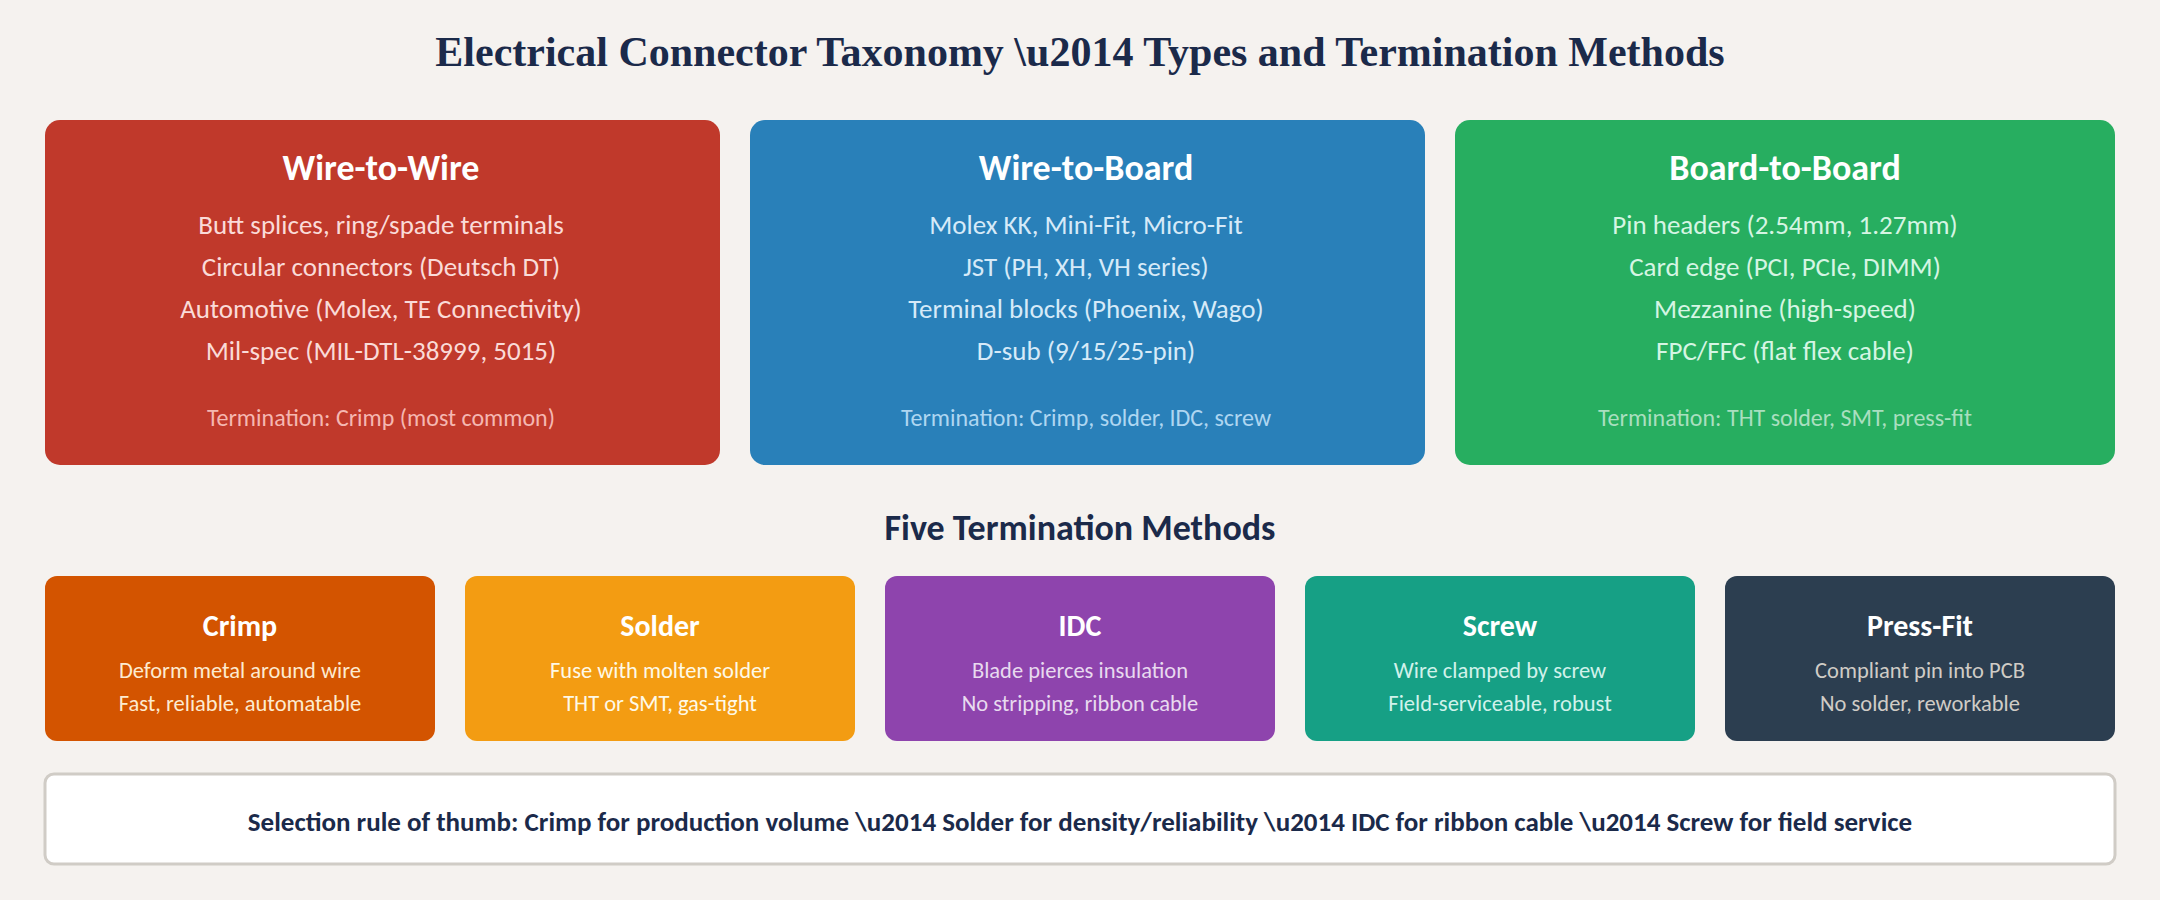
\includegraphics[width=\textwidth]{master_figs/fig1_connector_taxonomy.png}
\caption{Electrical connector taxonomy by connection type with five termination methods~[1],~[2].}
\label{fig:connector_taxonomy}
\end{figure}

\subsection{Harsh-Environment Connectors}

Students designing vehicle harnesses, outdoor systems, or launch hardware will encounter connectors engineered for abuse. Understanding the physical components of these systems is essential for specifying them correctly.

\textbf{Deutsch DT / DTM Series} (automotive/off-highway): These use a wedgelock that mechanically retains all contacts simultaneously, independent of the wire seal. Each cavity receives a silicone wire seal that grips the insulation OD, providing IP67/IP69K protection. Contacts are stamped-and-formed with a barrel crimp; the crimp must capture both the conductor and the insulation for strain relief. Deutsch connectors are the de facto standard for SAE Baja, Formula SAE, and agricultural equipment harnesses.

\textbf{MIL-DTL-38999 Series III} (aerospace/defense): A bayonet-coupled circular connector with a self-locking coupling ring that resists vibration. Uses machined contacts (not stamped) with interference-fit rear grommets for environmental sealing. Rated for extreme vibration (per MIL-STD-810), wide temperature ranges ($-65$ to $+200$\,\degC{}), and EMI shielding via conductive shell-to-shell contact. If your design involves launch hardware, flight systems, or classified defense work, 38999 is the starting point.

\textbf{Common to both}: Proper barrel crimps are critical; the crimp must form a gas-tight cold weld in the conductor barrel \emph{and} a secure grip in the insulation barrel. Using generic pliers instead of a calibrated ratchet tool produces crimps that look acceptable but fail under vibration or thermal cycling.


\subsection{Termination Methods}
\label{sec:termination}

The termination method is how the wire conductor is mechanically and electrically bonded to the connector contact. Each method involves different tools, skill levels, and performance characteristics.

\subsubsection{Crimp}

A precision die compresses a metal barrel around a stripped wire conductor, creating a gas-tight joint through cold-welding at the metal interface.

\begin{itemize}[nosep,leftmargin=1.5em]
  \item \textbf{Strengths}: Fast, repeatable, no heat required, excellent vibration resistance, gas-tight joint resists corrosion.
  \item \textbf{Limitations}: Requires calibrated crimp tools (hand ratchet or pneumatic); die must match the contact exactly. Poor crimps are invisible failures.
  \item \textbf{Best for}: Production wiring, automotive harnesses, harsh-environment connectors.
  \item \textbf{Quality verification}: Pull-test a sample of crimps per IPC/WHMA-A-620. Cross-section crimps periodically to verify cold-weld zone.
\end{itemize}

\begin{warningbox}[Pin Extraction: Use the Right Tool]
In prototype environments, students inevitably insert a contact into the wrong cavity. \textbf{Never} yank the wire or use a paperclip to extract a crimped pin; this damages the housing retention lance and the contact, creating an unreliable connection that will fail in service. Every connector family has a specific extraction tool (typically a thin-walled sleeve that depresses the retention lance). Keep the correct extraction tools on hand alongside your crimp tools; they cost a few dollars and save hours of rework and scrapped housings.
\end{warningbox}

\subsubsection{Solder}

Molten solder alloy (typically SAC305 lead-free or Sn63/Pb37) forms a metallurgical bond between wire and contact.

\begin{itemize}[nosep,leftmargin=1.5em]
  \item \textbf{Strengths}: Low contact resistance, well-understood process, easy visual inspection.
  \item \textbf{Limitations}: Requires heat (risk of insulation damage), not reworkable without desoldering tools, solder joints are brittle under vibration and thermal cycling.
  \item \textbf{Best for}: Board-level connections (through-hole and SMT), prototype wiring, low-vibration environments.
\end{itemize}

\subsubsection{Insulation Displacement Contact (IDC)}

A sharp, slotted contact blade pierces through wire insulation and makes contact with the conductor, all in a single operation.

\begin{itemize}[nosep,leftmargin=1.5em]
  \item \textbf{Strengths}: Extremely fast, no stripping required, good for mass-termination of ribbon cables.
  \item \textbf{Limitations}: Limited to small wire gauges (typically 22--28~AWG), not suitable for high-vibration environments, contact can relax over time.
  \item \textbf{Best for}: Ribbon cable connectors, low-current signal wiring, internal PCB connections.
\end{itemize}

\subsubsection{Screw Terminal}

A screw clamp compresses the wire conductor against a metal plate or barrel inside the terminal block.

\begin{itemize}[nosep,leftmargin=1.5em]
  \item \textbf{Strengths}: Tool-free or simple screwdriver, field-serviceable, wide wire gauge range, easy to inspect.
  \item \textbf{Limitations}: Bulky, screws can loosen under vibration, relatively high contact resistance compared to crimp.
  \item \textbf{Best for}: Panel-mount terminal blocks, DIN-rail wiring, power distribution, industrial controls.
\end{itemize}

\subsubsection{Press-Fit (Compliant Pin)}

A specially shaped contact pin (often an ``eye-of-needle'' or ``action pin'' geometry) is pressed into a plated through-hole on a PCB, creating a gas-tight interference fit.

\begin{itemize}[nosep,leftmargin=1.5em]
  \item \textbf{Strengths}: No solder required, excellent reliability, eliminates solder joint fatigue, good for backplane connectors.
  \item \textbf{Limitations}: Requires controlled insertion force and tooling, board must have proper hole tolerances, not field-reworkable.
  \item \textbf{Best for}: Backplane connectors, automotive ECU headers, high-reliability board-level connections.
\end{itemize}

\begin{tipbox}[Termination Method Selection Summary]

\end{tipbox}

\begin{figure}[htbp]
\centering
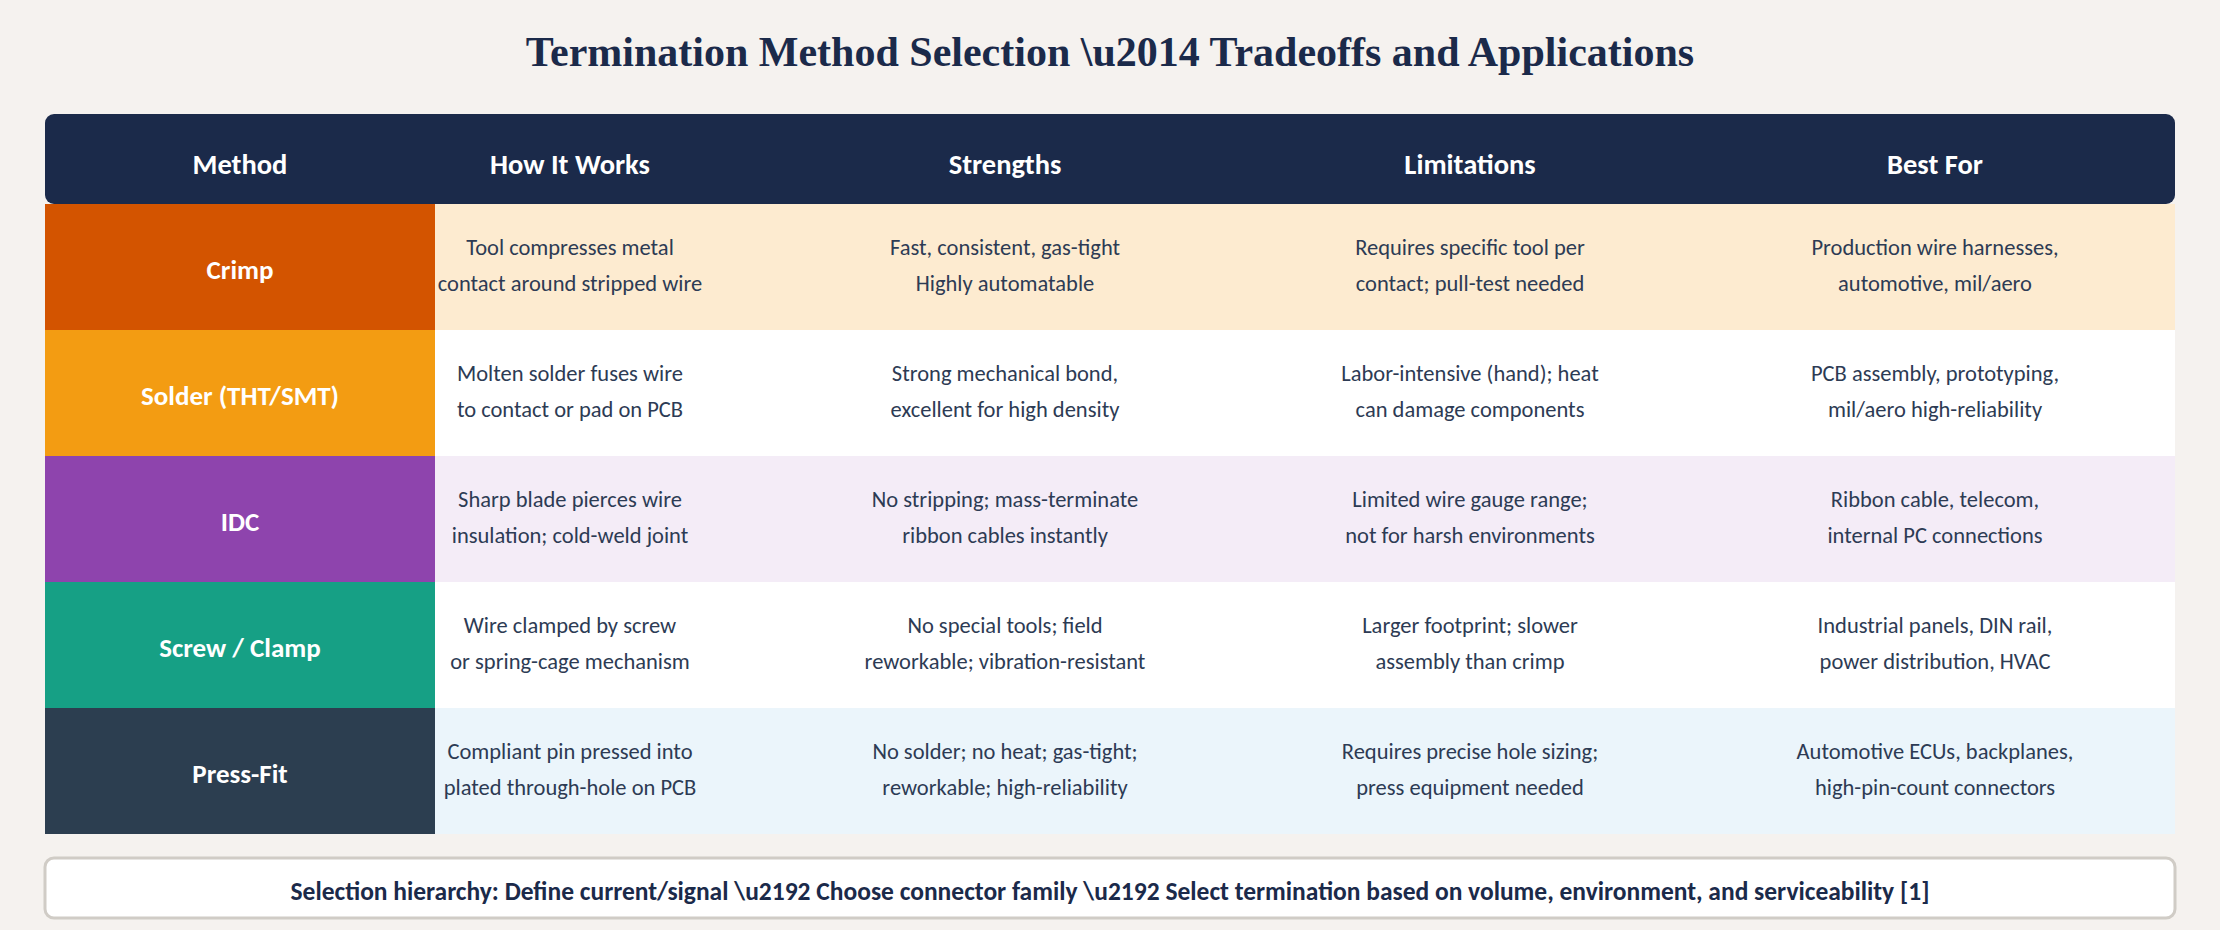
\includegraphics[width=\textwidth]{master_figs/fig2_termination_matrix.png}
\caption{Termination tradeoff matrix; mechanism, strengths, limitations, and best applications~[1],~[2].}
\label{fig:termination_matrix}
\end{figure}


\subsection{Key Electrical Specifications}
\label{sec:elecspecs}

When specifying an electrical connector in your design documentation, you must define each of the following parameters.

\subsubsection{Current Rating}

The maximum continuous current per contact, in amperes. This depends on contact size, material, plating type, and number of loaded contacts. 

\begin{warningbox}[Thermal Derating]
Always derate for multi-pin loaded connectors. When adjacent contacts all carry current, thermal stacking raises the temperature inside the housing, reducing each contact's effective capacity. A connector rated at 10\,A per contact at 25\,\degC{} may only safely handle 7\,A per contact at 85\,\degC{} ambient. Manufacturers provide derating curves; never ignore them.
\end{warningbox}

\begin{tipbox}[Bridging to Wire Selection (AWG)]
The connector's current rating sets the \emph{minimum} wire gauge you can use. Standard practice: select wire whose ampacity (per NEC Table~310.16 or MIL-W-22759 for aerospace) meets or exceeds the derated connector contact rating. Common reference points for chassis wiring in free air at 30\,\degC{}: 22~AWG $\approx$ 7\,A, 18~AWG $\approx$ 10\,A, 16~AWG $\approx$ 13\,A, 14~AWG $\approx$ 17\,A, 12~AWG $\approx$ 23\,A, 10~AWG $\approx$ 33\,A. Always verify that the connector contact accepts your chosen wire gauge; crimp contacts are rated for a specific AWG range (e.g., 18--22~AWG), and using the wrong gauge produces unreliable crimps.
\end{tipbox}

\subsubsection{Voltage Rating}

The maximum working voltage (VAC or VDC). This is determined by creepage (surface distance) and clearance (air gap) distances between adjacent contacts, as specified by IEC~61984~[2]. 

\textbf{Important}: Always specify the \emph{rated working voltage}, not the dielectric withstand (breakdown) voltage. Working voltage includes safety margin; breakdown voltage does not.

\subsubsection{Contact Resistance}

The electrical resistance measured across a mated contact pair, typically in milliohms (m$\Omega$). Gold-plated contacts achieve $<$20\,m$\Omega$; tin-plated contacts may range from 20--50\,m$\Omega$ when new.

\textbf{Why it matters}: At 10\,A, even 50\,m$\Omega$ of contact resistance produces:
\begin{equation}
  P = I^2 R = (10)^2 \times 0.050 = 0.5\,W \text{ of heat per contact}
\end{equation}
Contact resistance increases with mating cycles and in corrosive environments. Always verify with a milliohm meter during commissioning.

\subsubsection{IP Rating (Ingress Protection)}

Defined by IEC~60529~[3], the IP code uses two digits:
\begin{itemize}[nosep,leftmargin=1.5em]
  \item \textbf{First digit (0--6)}: Protection against solid objects, from ``no protection'' (0) to ``dust-tight'' (6).
  \item \textbf{Second digit (0--9K)}: Protection against liquids, from ``no protection'' (0) to ``high-pressure, high-temperature washdown'' (9K).
\end{itemize}

\begin{table}[htbp]
\centering
\small
\begin{tabular}{c l l}
  \toprule
  \textbf{IP Rating} & \textbf{Meaning} & \textbf{Typical Application} \\
  \midrule
  IP20 & Finger-safe; no liquid protection & Indoor panel wiring \\
  IP54 & Dust-protected; splash-proof & General industrial \\
  IP67 & Dust-tight; 1\,m immersion for 30\,min & Outdoor, vehicle, marine \\
  IP68 & Dust-tight; continuous submersion & Submersible equipment \\
  IP69K & Dust-tight; high-pressure washdown & Food/pharma equipment \\
  \bottomrule
\end{tabular}
\caption{Common IP ratings and their applications.}
\end{table}

\subsubsection{Mating Cycles}

The rated number of connect/disconnect operations before mechanical or electrical degradation. Ranges vary enormously:
\begin{itemize}[nosep,leftmargin=1.5em]
  \item 25--50 cycles: permanent/semi-permanent installations.
  \item 500--1,000 cycles: periodic maintenance access.
  \item 5,000--10,000+ cycles: test fixtures, instrumentation.
\end{itemize}
Gold plating significantly outlasts tin plating. Contact wear directly increases resistance over mating life.


\subsection{Electrical Connector Failure Modes}
\label{sec:elecfailure}

Understanding failure modes is essential for designing robust connections. These are listed roughly in order of how commonly they cause problems in practice.

\subsubsection{Fretting Corrosion}

\textbf{Mechanism}: Micro-motion from vibration (amplitudes as small as 10\,$\mu$m) wears through the contact plating, exposing base metal. Oxides form on the exposed metal, creating high-resistance debris particles that accumulate at the contact interface.

\textbf{Why it's dangerous}: Fretting corrosion is the most insidious failure mode because it develops slowly, manifests as intermittent contact, and is difficult to diagnose. Resistance may fluctuate between normal and open-circuit depending on vibration state.

\textbf{Mitigations}:
\begin{itemize}[nosep,leftmargin=1.5em]
  \item Gold plating (resists oxide formation).
  \item Higher contact normal force (resists micro-motion).
  \item Strain-relief on cables (reduces transmitted vibration).
  \item Secondary locking features on connectors.
\end{itemize}

\begin{figure}[htbp]
\centering
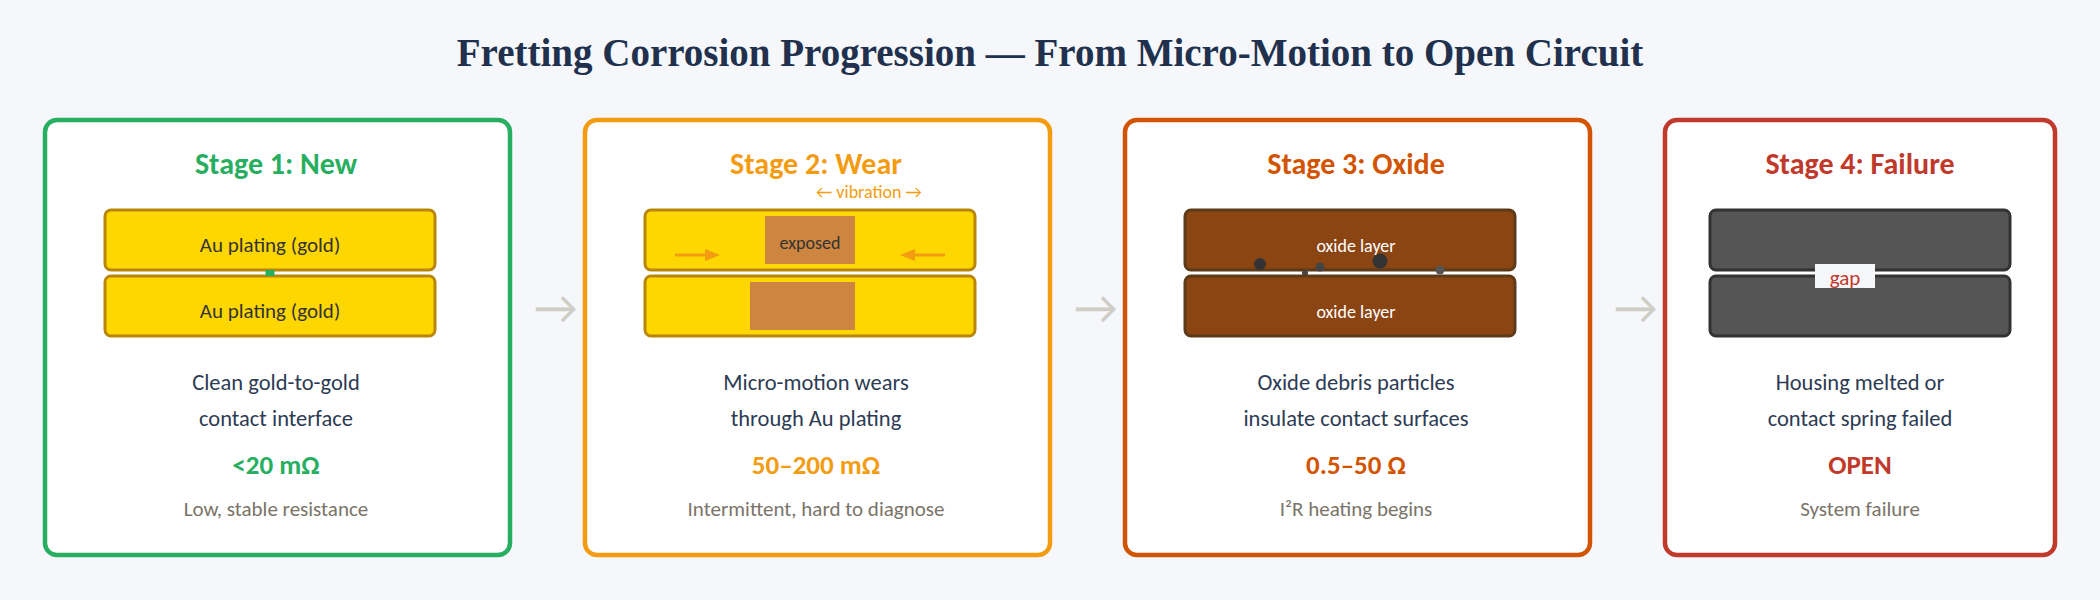
\includegraphics[width=\textwidth]{master_figs/fig7_fretting_progression.png}
\caption{Fretting corrosion progression, from clean gold-plated contacts through oxide accumulation to open-circuit failure. Note resistance escalation across stages.}
\label{fig:fretting_progression}
\end{figure}

Figure~\ref{fig:fretting_progression} illustrates the four-stage progression of fretting corrosion.  At Stage~1, clean gold-plated contacts exhibit stable resistance below 20\,m$\Omega$. Vibration-induced micro-motion gradually wears through the plating at Stage~2, intermittently exposing base metal and raising resistance to 50--200\,m$\Omega$, often misdiagnosed as a ``loose connection.'' By Stage~3, accumulated oxide debris insulates the contact surfaces, resistance climbs to the ohm range, and $I^2R$ heating accelerates further degradation. Stage~4 is outright failure: melted housing, collapsed contact springs, or open circuit. Because Stage~2 symptoms are intermittent and position-dependent, fretting often passes bench-top continuity checks only to fail under dynamic load, a pattern students must learn to recognize.

\subsubsection{Overheating ($I^2 R$ Heating)}

\textbf{Mechanism}: Exceeding the current rating causes resistive heating at the contact interface. Heat accumulates in the housing, softening thermoplastic materials and potentially igniting adjacent insulation or components.

\textbf{Mitigations}:
\begin{itemize}[nosep,leftmargin=1.5em]
  \item Never exceed rated current; derate for ambient temperature.
  \item Select contacts with lower resistance (gold plating, larger cross-section).
  \item Distribute high currents across multiple contacts.
\end{itemize}

\subsubsection{Creep and Stress Relaxation}

\textbf{Mechanism}: Contact springs gradually lose their clamping force at elevated temperatures. The contact normal force decreases over time, increasing resistance and accelerating other failure modes.

\textbf{Mitigations}:
\begin{itemize}[nosep,leftmargin=1.5em]
  \item Specify beryllium copper (BeCu) contacts for any application above 60\,\degC{} continuous. BeCu resists creep far better than brass or phosphor bronze.
  \item Overspecify contact normal force for high-temperature applications.
\end{itemize}

\subsubsection{Moisture Ingress}

\textbf{Mechanism}: Water bridges between contacts, causing electrochemical corrosion, increased resistance, or direct short circuits.

\textbf{Mitigations}:
\begin{itemize}[nosep,leftmargin=1.5em]
  \item Specify appropriate IP rating per IEC~60529~[3].
  \item Use sealed connectors with O-ring face seals and wire seals for any outdoor, vehicle, or washdown application.
  \item Apply conformal coating on exposed PCB connections.
\end{itemize}


% ══════════════════════════════════════════════════════════════════════
\section{Fluid System Connectors}
% ══════════════════════════════════════════════════════════════════════

\subsection{Threaded Pipe Fitting Standards}

Two incompatible tapered thread standards dominate global pipe fitting. Geography determines which you encounter.

\subsubsection{NPT: National Pipe Taper (ASME B1.20.1)}

\begin{itemize}[leftmargin=1.5em]
  \item \textbf{Thread angle}: \ang{60} with pointed crests and roots.
  \item \textbf{Taper}: 1:16 (\textonequarter\,inch per inch of thread length, equivalent to \textthreequarters\,inch per foot).
  \item \textbf{Sealing mechanism}: Thread interference creates a metal-to-metal wedge seal. Because the thread form has clearance at crests and roots, NPT joints \emph{always} require supplemental sealing; either PTFE (Teflon) tape or anaerobic pipe dope.
  \item \textbf{NPTF variant}: ``Dryseal'' NPT uses a modified thread form with tighter root/crest tolerances that crushes metal at the interface, theoretically sealing without sealant. In practice, sealant is still recommended.
  \item \textbf{Size range}: 1/8\,in.\ to 24\,in.\ nominal pipe size (NPS).
  \item \textbf{Pressure rating}: Up to 15000\,psi depending on material and size.
  \item \textbf{Geography}: Dominant in the United States and Canada.
\end{itemize}

\subsubsection{BSP: British Standard Pipe (ISO 228 / ISO 7-1)}

\begin{itemize}[leftmargin=1.5em]
  \item \textbf{Thread angle}: \ang{55} Whitworth form with rounded crests and roots.
  \item \textbf{Two sub-types}:
  \begin{itemize}[nosep]
    \item \textbf{BSPT} (designation ``R''): Tapered threads, seals like NPT via thread interference plus sealant.
    \item \textbf{BSPP} (designation ``G''): Parallel (straight) threads that \emph{do not} seal on the threads. Sealing is achieved with a bonded washer or O-ring compressed against a flat face.
  \end{itemize}
  \item \textbf{Size range}: 1/8\,in.\ to 6\,in.\ (inch-denominated but used globally outside North America).
  \item \textbf{Pressure rating}: Up to 6000\,psi typical.
  \item \textbf{Geography}: Dominant in Europe, Asia, and most of the world outside North America.
\begin{warningbox}[The Point of No Return: Thread Galling]
NPT threads are tapered at 60\degC{}. BSP threads are tapered at 55\degC{}. A 55\degC{} BSP fitting \emph{will} start threading into a 60\degC{} NPT port---and then seize. In stainless steel, this produces \textbf{galling}: a cold-weld that permanently fuses the two components. Both parts become scrap metal. There is no recovery.

\textbf{The Finger Test}: before applying any wrench, thread the fitting by hand. If you cannot achieve at least \textbf{three full turns by finger pressure alone}, STOP. The threads are incompatible, cross-threaded, or contaminated. Any attempt to force the connection with a wrench will result in irreversible damage. Verify the thread standard (NPT vs.\ BSP), clean both threads, apply appropriate sealant (Teflon tape for NPT, bonded washer for BSP parallel), and try again.
\end{warningbox}
\end{itemize}


\begin{warningbox}[Thread Galling: The Point of No Return]
In stainless steel or aluminum, forcing a mismatched or cross-threaded fitting with a wrench causes \textbf{galling}; a cold-weld that permanently destroys both components. Once galling begins, reaching for a bigger wrench turns a \$50 component into a \$100 mistake (two destroyed parts plus the replacement).

\textbf{The Finger Test}: if you cannot thread a fitting at least three full turns by hand, \textbf{STOP}. You are either cross-threaded or mixing thread standards. No amount of force or sealant can fix galled threads.

\textbf{Prevention for stainless-on-stainless connections}: apply nickel-based anti-seize compound (e.g., Permatex Nickel Anti-Seize or Loctite LB 8023) to the male threads before assembly. Anti-seize reduces friction and prevents the metal-to-metal adhesion that initiates galling. This is mandatory for any stainless steel fluid fitting in your design.
\end{warningbox}

\begin{warningbox}[Critical Incompatibility]
NPT (\ang{60} pointed threads) and BSP (\ang{55} rounded threads) are \textbf{NOT} interchangeable. They may appear to engage for a few turns but will not seal properly. Cross-threading causes galling, thread damage, and leaks that may develop catastrophically under pressure. \textbf{Always} verify thread standard with a thread pitch gauge before assembly.
\end{warningbox}

\begin{table}[htbp]
\centering
\small
\begin{tabularx}{\textwidth}{l X X}
  \toprule
  \textbf{Feature} & \textbf{NPT (ASME B1.20.1)} & \textbf{BSP (ISO 228 / ISO 7-1)} \\
  \midrule
  Thread angle & \ang{60}, pointed crests/roots & \ang{55} Whitworth, rounded crests/roots \\
  Taper & 1:16 (all NPT tapered) & BSPT tapered; BSPP parallel \\
  Sealing & Thread interference + sealant & BSPT: thread + sealant; BSPP: washer/O-ring \\
  Geography & U.S., Canada & Europe, Asia, rest of world \\
  Max pressure & 15000\,psi & 6000\,psi typical \\
  \bottomrule
\end{tabularx}
\caption{NPT vs.\ BSP thread comparison.}
\end{table}

\begin{figure}[htbp]
\centering
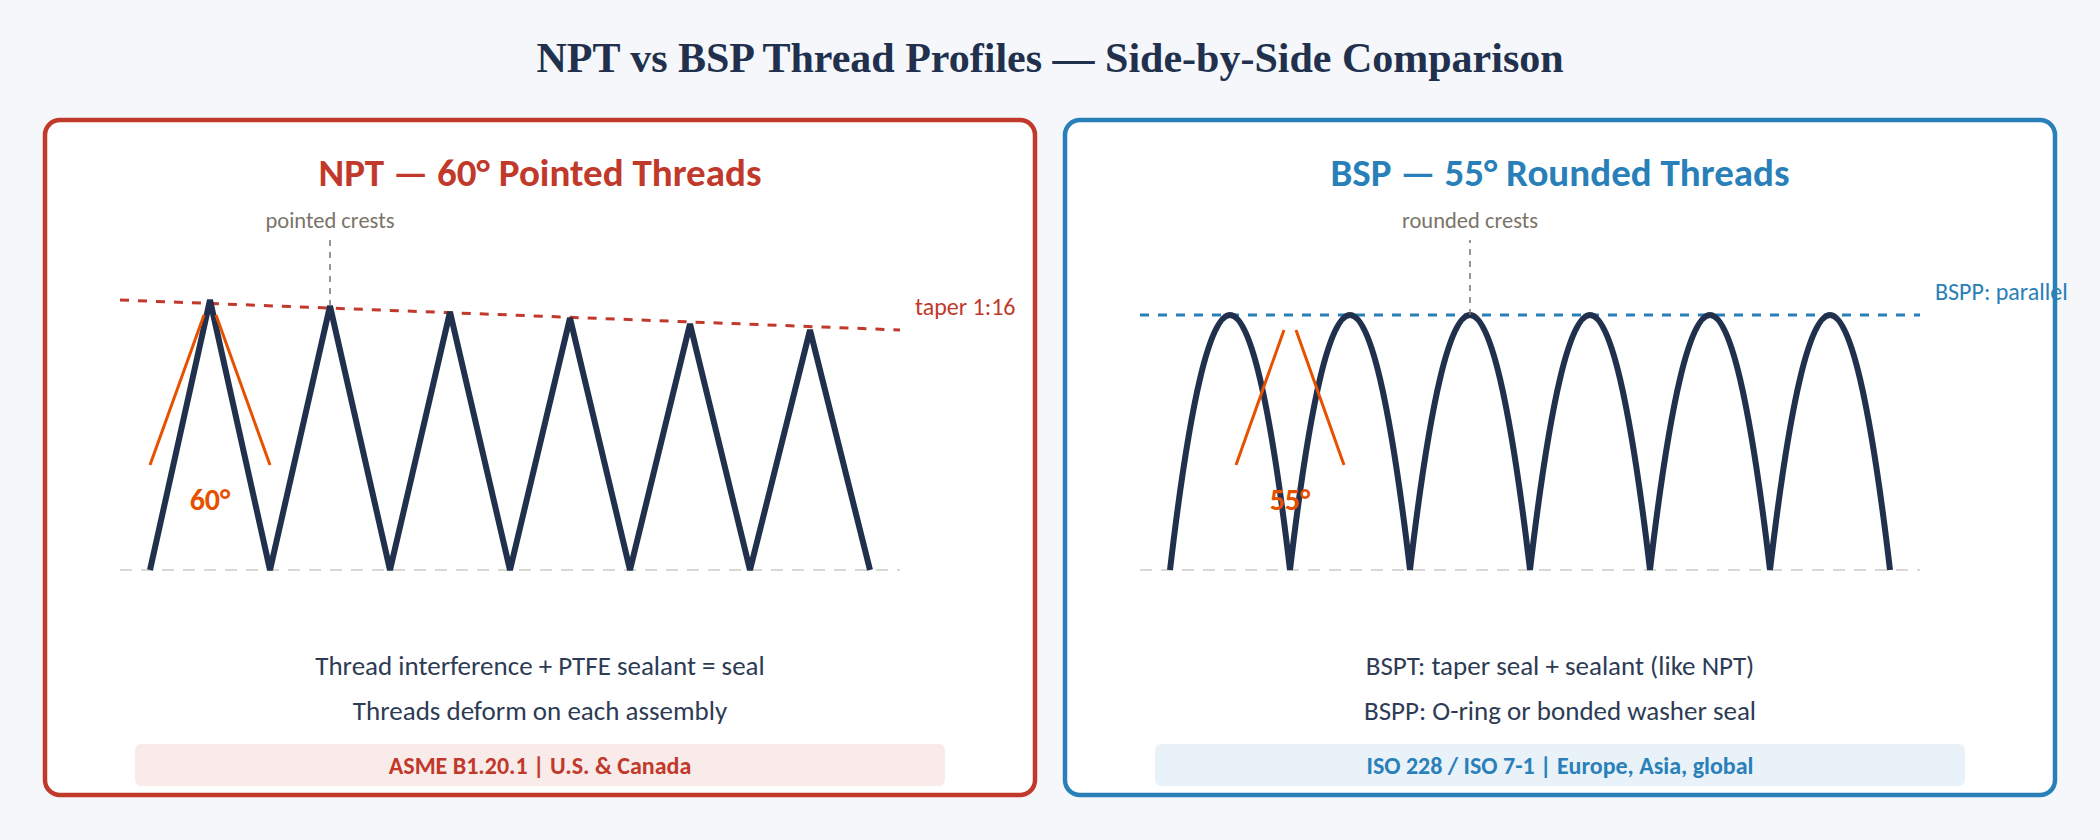
\includegraphics[width=\textwidth]{master_figs/fig5_thread_profiles.png}
\caption{NPT vs.\ BSP thread profiles; note the pointed \ang{60} crests on NPT versus the rounded \ang{55} Whitworth crests on BSP. These subtle geometric differences make the two standards completely incompatible.}
\label{fig:thread_profiles}
\end{figure}

Figure~\ref{fig:thread_profiles} places the two thread forms side by side so the geometric distinction is immediately visible. NPT's \ang{60} pointed crests create a wedging action as the taper engages; metal deforms at each assembly, which is why PTFE sealant is required and why each reassembly cycle slightly degrades the thread. BSP's \ang{55} Whitworth form uses rounded crests that are less prone to galling but follow an entirely different pitch schedule. The BSPP (parallel) variant does not seal on the thread at all; the thread merely provides clamping force while an O-ring or bonded washer creates the pressure boundary against a flat face. This is a critical distinction: applying PTFE tape to a BSPP fitting is a common student mistake that serves no purpose and can actually prevent proper washer compression.


\subsection{Tube Fittings and Quick-Connect Couplings}

Unlike threaded pipe fittings (which connect pipes), tube fittings connect \emph{tubing}; a product specified by outside diameter (OD) and wall thickness, with tighter dimensional tolerances than pipe.

\subsubsection{JIC 37$^{\circ}$\ Flare (SAE J514)}

The tube end is flared to a \ang{37} cone that mates with a matching seat in the fitting body. The joint seals metal-to-metal; no sealant, tape, or elastomeric seal is required. The fitting uses a straight (non-tapered) thread; the thread provides clamping force only and does not contribute to sealing.

\begin{itemize}[nosep,leftmargin=1.5em]
  \item Reassemblable without degradation (unlike taper threads which deform with each assembly).
  \item The hydraulic industry standard worldwide.
  \item Pressure ratings to 10000\,psi.
  \item AN (Army--Navy) fittings are the military equivalent of JIC, with identical \ang{37} geometry.
\end{itemize}

\subsubsection{Compression Fittings (Swagelok-type)}

One or two ferrules (metal rings) are swaged (compressed) onto the tube OD when the nut is tightened. The ferrule bites into the tube, creating both a grip and a seal.

\begin{itemize}[nosep,leftmargin=1.5em]
  \item No welding, brazing, flaring, or special tools required.
  \item Tube OD is the sizing basis (1/4\,in., 3/8\,in., 1/2\,in., etc.).
  \item \textbf{Gaugeable}: Many designs include a visual indicator (gap gauge) so you can verify proper assembly by inspection.
  \item Pressure ratings up to 20000\,psi for medium-pressure configurations.
  \item Brands: Swagelok, Parker CPI/A-LOK, Ham-Let.
\end{itemize}

\subsubsection{Push-to-Connect}

The tube pushes into the fitting body. An internal collet (toothed ring) grips the tube OD, and an O-ring provides the seal. Assembly is one-handed and tool-free.

\begin{itemize}[nosep,leftmargin=1.5em]
  \item Common in pneumatics (air systems), typically up to $\$\sim\$$250\,psi.
  \item Common brands: SMC, Festo, John Guest.
  \item Fast assembly but limited to lower pressures and non-critical sealing applications.
\end{itemize}

\subsubsection{Quick-Disconnect (QD) Couplings}

Two halves, a plug and a socket, connect and disconnect by hand, often with a locking sleeve or collar. Self-sealing valves in one or both halves prevent fluid loss on disconnect.

\begin{itemize}[nosep,leftmargin=1.5em]
  \item \textbf{Flat-face}: Minimal fluid spillage on disconnect, used in clean or environmentally sensitive applications.
  \item \textbf{Poppet-valve}: Spring-loaded valve seals on disconnect, less expensive but more spillage.
  \item Common applications: hydraulic tool circuits, coolant loops, test equipment.
\end{itemize}

\begin{table}[htbp]
\centering
\small
\begin{tabularx}{\textwidth}{l c c X}
  \toprule
  \textbf{Fitting Family} & \textbf{Pressure} & \textbf{Seal Type} & \textbf{Key Characteristic} \\
  \midrule
  JIC 37$^{\circ}$\ Flare & 10000\,psi & Metal-to-metal & Reassemblable; hydraulic standard \\
  Compression & 20000\,psi & Ferrule swage & No special tools; gaugeable \\
  Push-to-Connect & 250\,psi & O-ring & Tool-free; pneumatics \\
  Quick-Disconnect & Varies & Valve + O-ring & Hand-connect; self-sealing \\
  \bottomrule
\end{tabularx}
\caption{Tube fitting and coupling comparison.}
\end{table}

\begin{figure}[htbp]
\centering
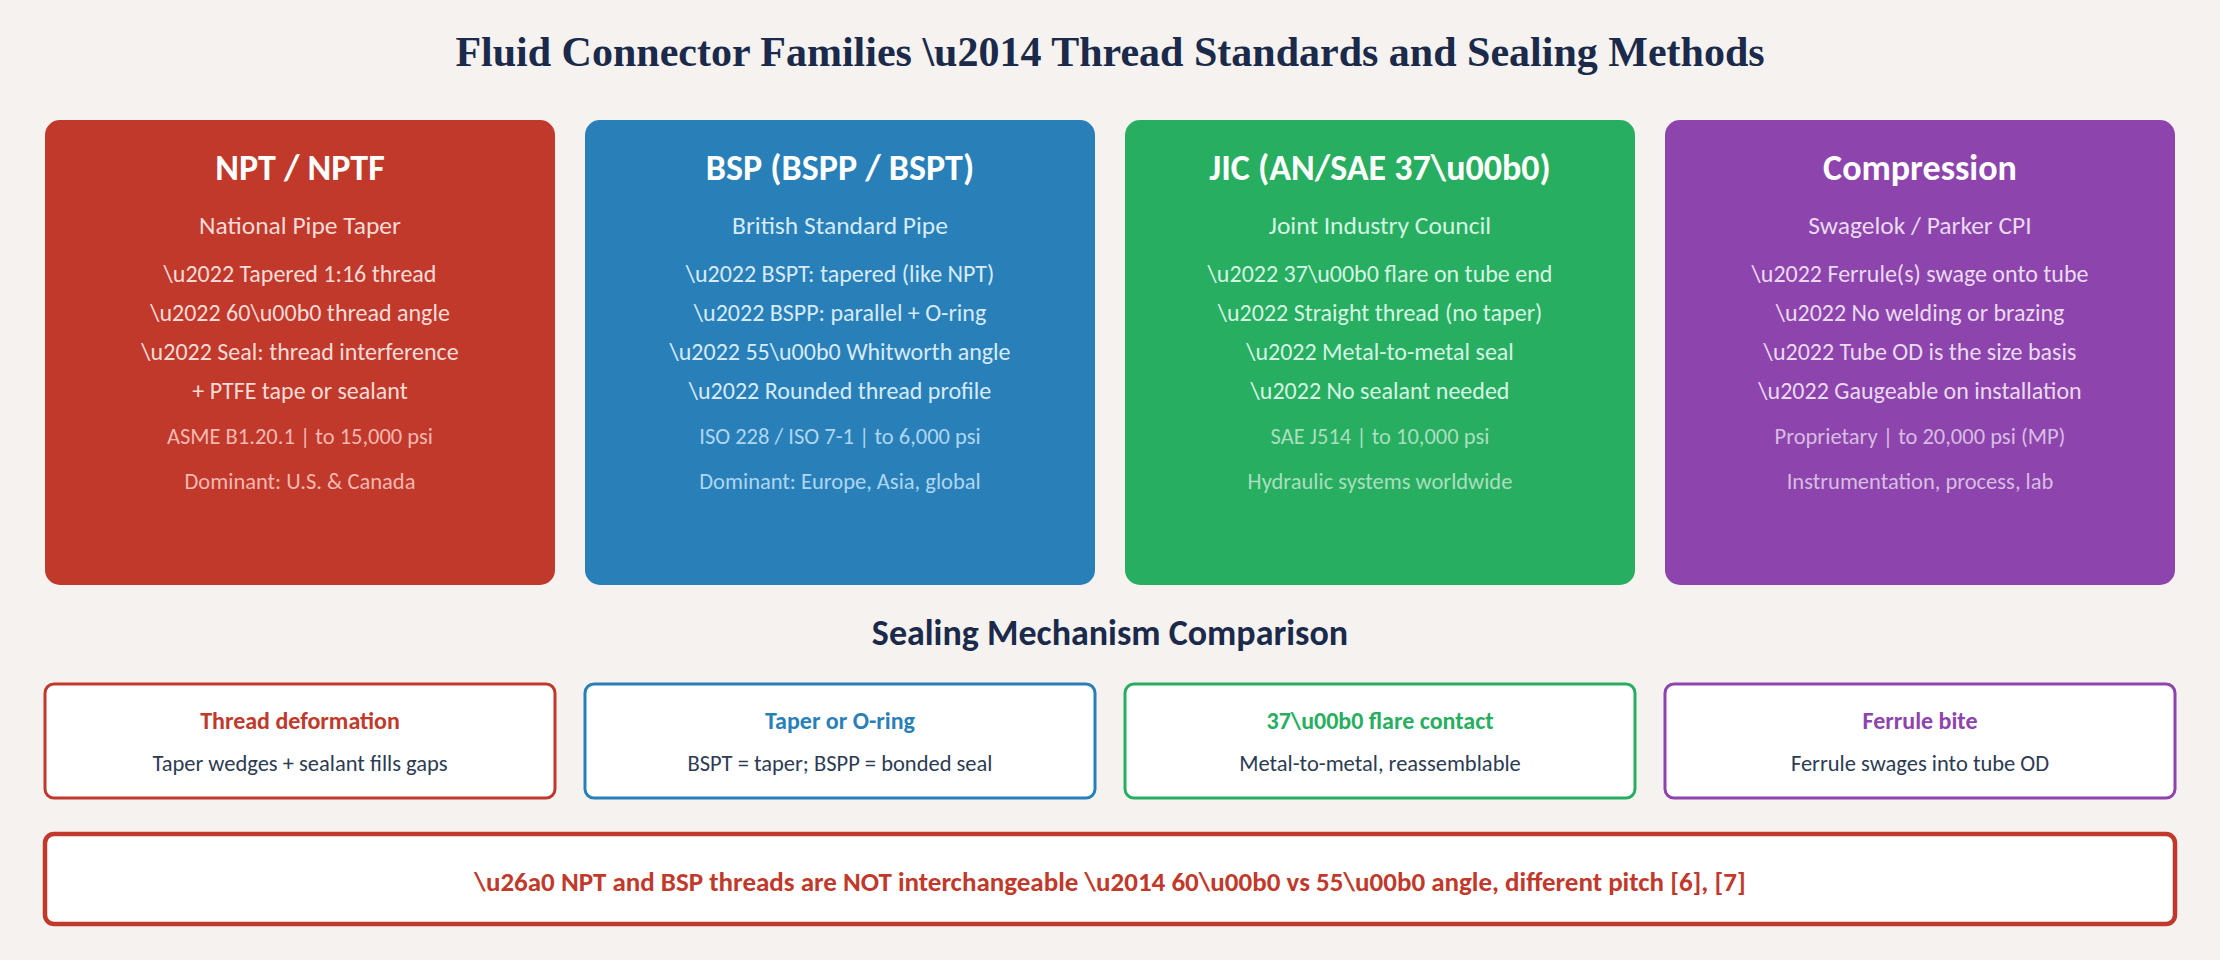
\includegraphics[width=\textwidth]{master_figs/fig3_fluid_connectors.png}
\caption{Four major fluid connector families with thread standards, pressure ratings, and sealing mechanisms.}
\label{fig:fluid_connectors}
\end{figure}

\begin{figure}[htbp]
\centering
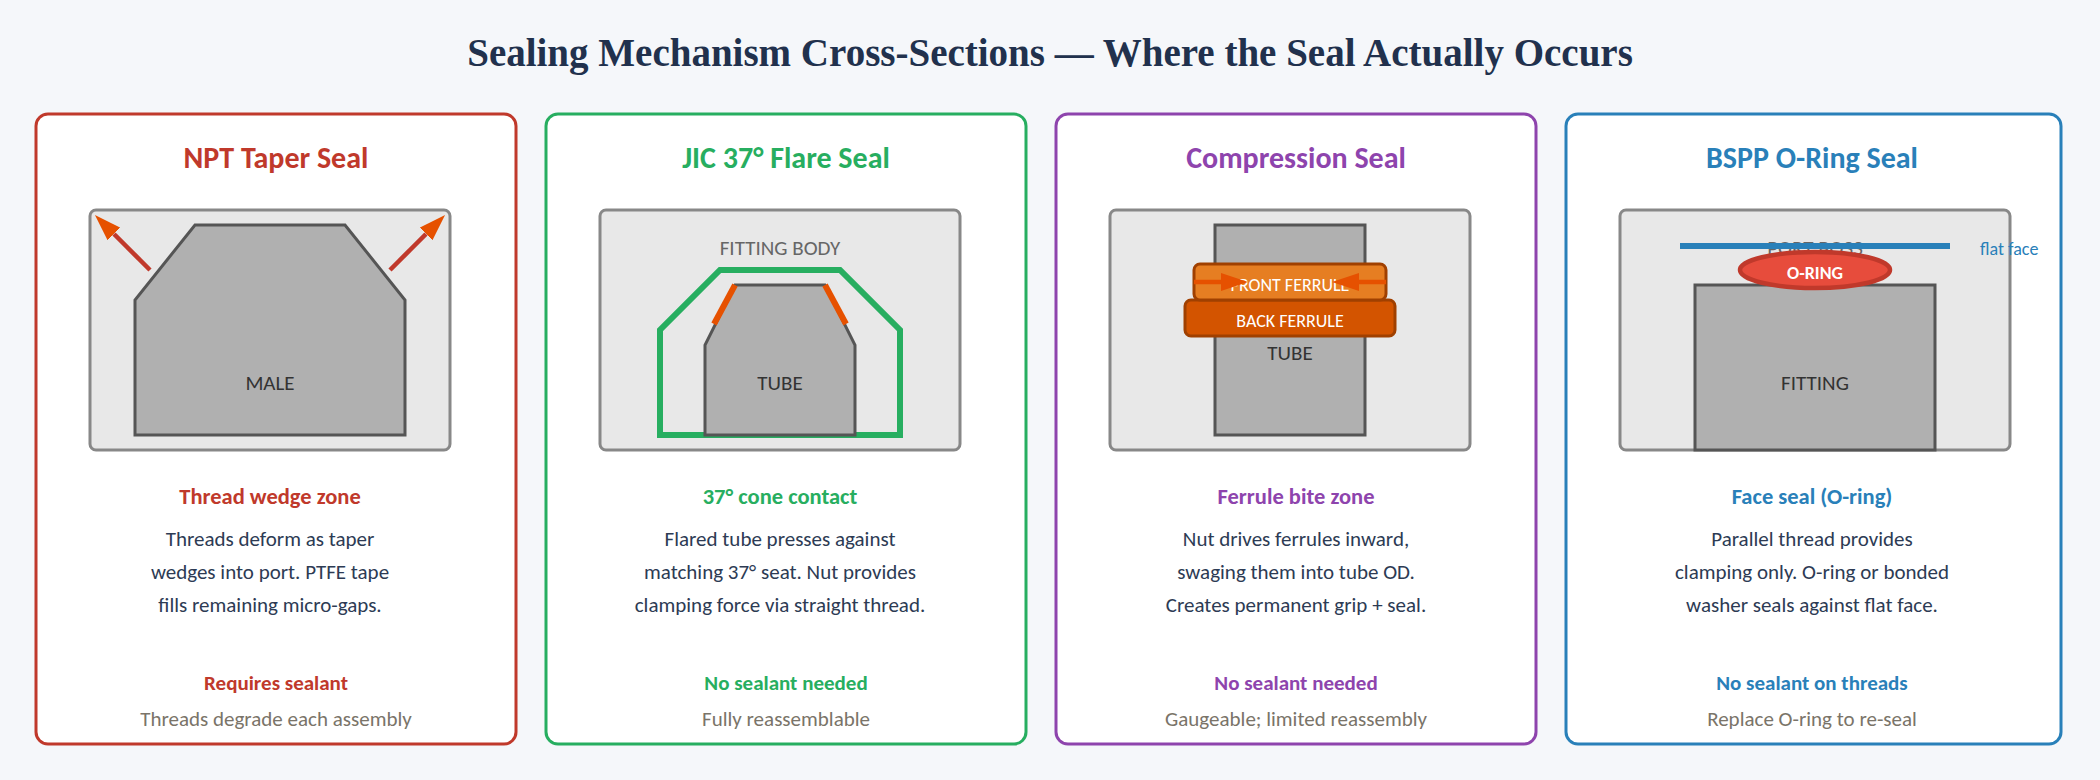
\includegraphics[width=\textwidth]{master_figs/fig6_seal_cross_sections.png}
\caption{Sealing mechanism cross-sections showing exactly where each seal forms: NPT thread wedge, JIC \ang{37} flare cone contact, compression ferrule bite zone, and BSPP face-seal O-ring.}
\label{fig:seal_cross_sections}
\end{figure}

Figure~\ref{fig:seal_cross_sections} shows the internal geometry of each sealing method so students can visualize \emph{why} proper torque and assembly procedures matter. In the NPT taper seal, the thread flanks themselves deform to create a pressure boundary, which is why sealant is mandatory to fill the remaining micro-gaps and why repeated assembly progressively damages the seal surfaces. In the JIC \ang{37} flare, the cone-shaped tube end presses against a matching seat in the fitting body; the straight thread provides clamping force only. This metal-to-metal geometry is fully reassemblable because the sealing surfaces do not deform. In compression fittings, the front ferrule bites radially into the tube OD while the back ferrule provides axial grip; the nut drives both ferrules during initial makeup. Once swaged, the ferrule is permanently deformed, which limits reassembly. In the BSPP face seal, the parallel thread clamps the fitting against the port face while an O-ring in a groove creates the pressure boundary, the thread contributes zero sealing.


\subsection{Key Fluid Connector Specifications}
\label{sec:fluidspecs}

When specifying a fluid connector in your design documentation, define each of the following.

\subsubsection{Working Pressure}

The maximum continuous operating pressure (psi or bar). Always specify \emph{working} pressure, not burst pressure. Standard safety factors:
\begin{itemize}[nosep,leftmargin=1.5em]
  \item Hydraulic: burst $\geq 4\times$ working.
  \item Pneumatic: burst $\geq 3\times$ working.
  \item \textbf{Design rule}: Never operate above 25\% of burst pressure.
\end{itemize}

\subsubsection{Temperature Range}

Temperature determines seal material selection:

\begin{table}[htbp]
\centering
\small
\begin{tabularx}{\textwidth}{l c X}
  \toprule
  \textbf{Seal Material} & \textbf{Range} & \textbf{Notes} \\
  \midrule
  Buna-N (Nitrile, NBR) & $-40$ to 250\,$^{\circ}$F & General purpose; petroleum-compatible \\
  Viton (FKM) & $-20$ to 400\,$^{\circ}$F & Chemical resistance; fuel systems \\
  PTFE (Teflon) & $-100$ to 500\,$^{\circ}$F & Widest range; chemically inert; no elasticity \\
  EPDM & $-65$ to 300\,$^{\circ}$F & Steam/water service; not oil-compatible \\
  \bottomrule
\end{tabularx}
\caption{Seal material temperature ranges and applications.}
\end{table}

Always verify seal compatibility with both the fluid \emph{and} the operating temperature.

\subsubsection{Fluid Compatibility}

Verify fitting body material and seal material against the working fluid using manufacturer chemical compatibility charts:
\begin{itemize}[nosep,leftmargin=1.5em]
  \item \textbf{Stainless steel}: Resists most chemicals; highest cost.
  \item \textbf{Brass}: Common for water, air, and general service; not for ammonia or acetylene.
  \item \textbf{Carbon steel}: Standard for hydraulic oil systems; requires corrosion protection.
\end{itemize}

\subsubsection{Thread / Tube Size}

\begin{itemize}[nosep,leftmargin=1.5em]
  \item \textbf{Threaded fittings}: Specified by Nominal Pipe Size (NPS). Note that NPS does \emph{not} equal the actual outside diameter. For example, 1/2\,in.\ NPS pipe has an OD of 0.840\,in.
  \item \textbf{Tube fittings}: Specified by tube outside diameter (OD). Common sizes: 1/4\,in., 3/8\,in., 1/2\,in.
  \item \textbf{Always measure with calipers and thread gauges}. Never assume a size by visual inspection.
\end{itemize}

\subsubsection{End Configuration}

Select the geometry that connects the fitting to your system: straight, elbow (45$^{\circ}$\ or 90$^{\circ}$), tee, cross, union, reducer, or bulkhead. 

\begin{tipbox}[Minimize Joints]
Every fitting joint is a potential leak point. Design your routing to minimize the total number of fittings in a line. Avoid stacking street elbows in series; use a single 90$^{\circ}$\ elbow or a pre-bent tube run instead.
\end{tipbox}


\subsection{Fluid Connector Failure Modes}
\label{sec:fluidfailure}

\subsubsection{Cross-Threading}

\textbf{Mechanism}: Attempting to mate NPT into BSP (or vice versa), or even same-standard threads started at an angle, destroys thread profiles and causes immediate or delayed leaks.

\textbf{Mitigations}:
\begin{itemize}[nosep,leftmargin=1.5em]
  \item Always verify thread standard with a thread pitch gauge before assembly.
  \item Start threads by hand for at least two full turns before applying a wrench.
  \item NPT: \ang{60} pointed threads. BSP: \ang{55} rounded threads. They \emph{feel} similar but are not compatible.
\end{itemize}

\subsubsection{Over-Tightening}

\textbf{Mechanism}: Excessive torque cracks port bosses (especially aluminum and cast iron), deforms compression ferrules beyond recovery, and splits flare cones. Over-tightening destroys more fittings than under-tightening.

\textbf{Mitigations}:
\begin{itemize}[nosep,leftmargin=1.5em]
  \item Always use manufacturer-specified torque values.
  \item Use a calibrated torque wrench, not a ``feel'' wrench.
  \item For Swagelok-type fittings, follow the turns-past-finger-tight specification exactly.
\end{itemize}

\subsubsection{Seal Degradation}

\textbf{Mechanism}: O-rings and gaskets deteriorate from chemical attack (incompatible fluid), UV exposure, thermal cycling, and simple age. Seals swell, harden, crack, or take a permanent compression set.

\textbf{Mitigations}:
\begin{itemize}[nosep,leftmargin=1.5em]
  \item Establish replacement intervals based on seal material and service conditions.
  \item Keep spare seal kits on hand.
  \item Verify seal material compatibility with the fluid and temperature range before installation.
\end{itemize}

\subsubsection{Vibration Fatigue}

\textbf{Mechanism}: Cyclic stress at tube-to-fitting junctions nucleates fatigue cracks. Under pressure, these cracks propagate to failure; potentially a sudden, high-pressure fluid release.

\textbf{Mitigations}:
\begin{itemize}[nosep,leftmargin=1.5em]
  \item Use proper tube support clamps spaced per manufacturer recommendations.
  \item Route tubing to avoid sharp bends and unsupported cantilever lengths.
  \item Include flexible hose segments at vibration sources (pumps, engines).
\end{itemize}

\begin{warningbox}[High-Pressure Fluid Injection Injury]
A hydraulic line leak may be invisible; a pinhole stream at 2000\,psi can penetrate skin and inject fluid deep into tissue, causing catastrophic damage that requires emergency surgery within hours. \textbf{Never} check for hydraulic leaks by running a bare hand along a pressurized line. Use a piece of cardboard or a thermal camera instead. This is one of the most serious and least-understood hazards in hydraulic system work, and students designing or testing any pressurized fluid system must be explicitly aware of it before commissioning.
\end{warningbox}


% ══════════════════════════════════════════════════════════════════════
\section{Selection and Design Practice}
% ══════════════════════════════════════════════════════════════════════

\subsection{Connector Selection Logic}

Whether electrical or fluid, connector selection follows a universal logic sequence:

\begin{enumerate}[leftmargin=1.5em]
  \item \textbf{Rating}: What current, voltage, pressure, or flow must it handle?
  \item \textbf{Environment}: Temperature range, vibration, moisture/IP, chemical exposure?
  \item \textbf{Serviceability}: How often must it be connected/disconnected? What tools are available?
  \item \textbf{Cost}: What is the budget per connection, including tooling?
  \item \textbf{Standards}: Which industry/regulatory standards apply (IEC, SAE, ASME, MIL)?
  \item \textbf{Space}: What are the physical envelope constraints?
\end{enumerate}

\begin{figure}[htbp]
\centering
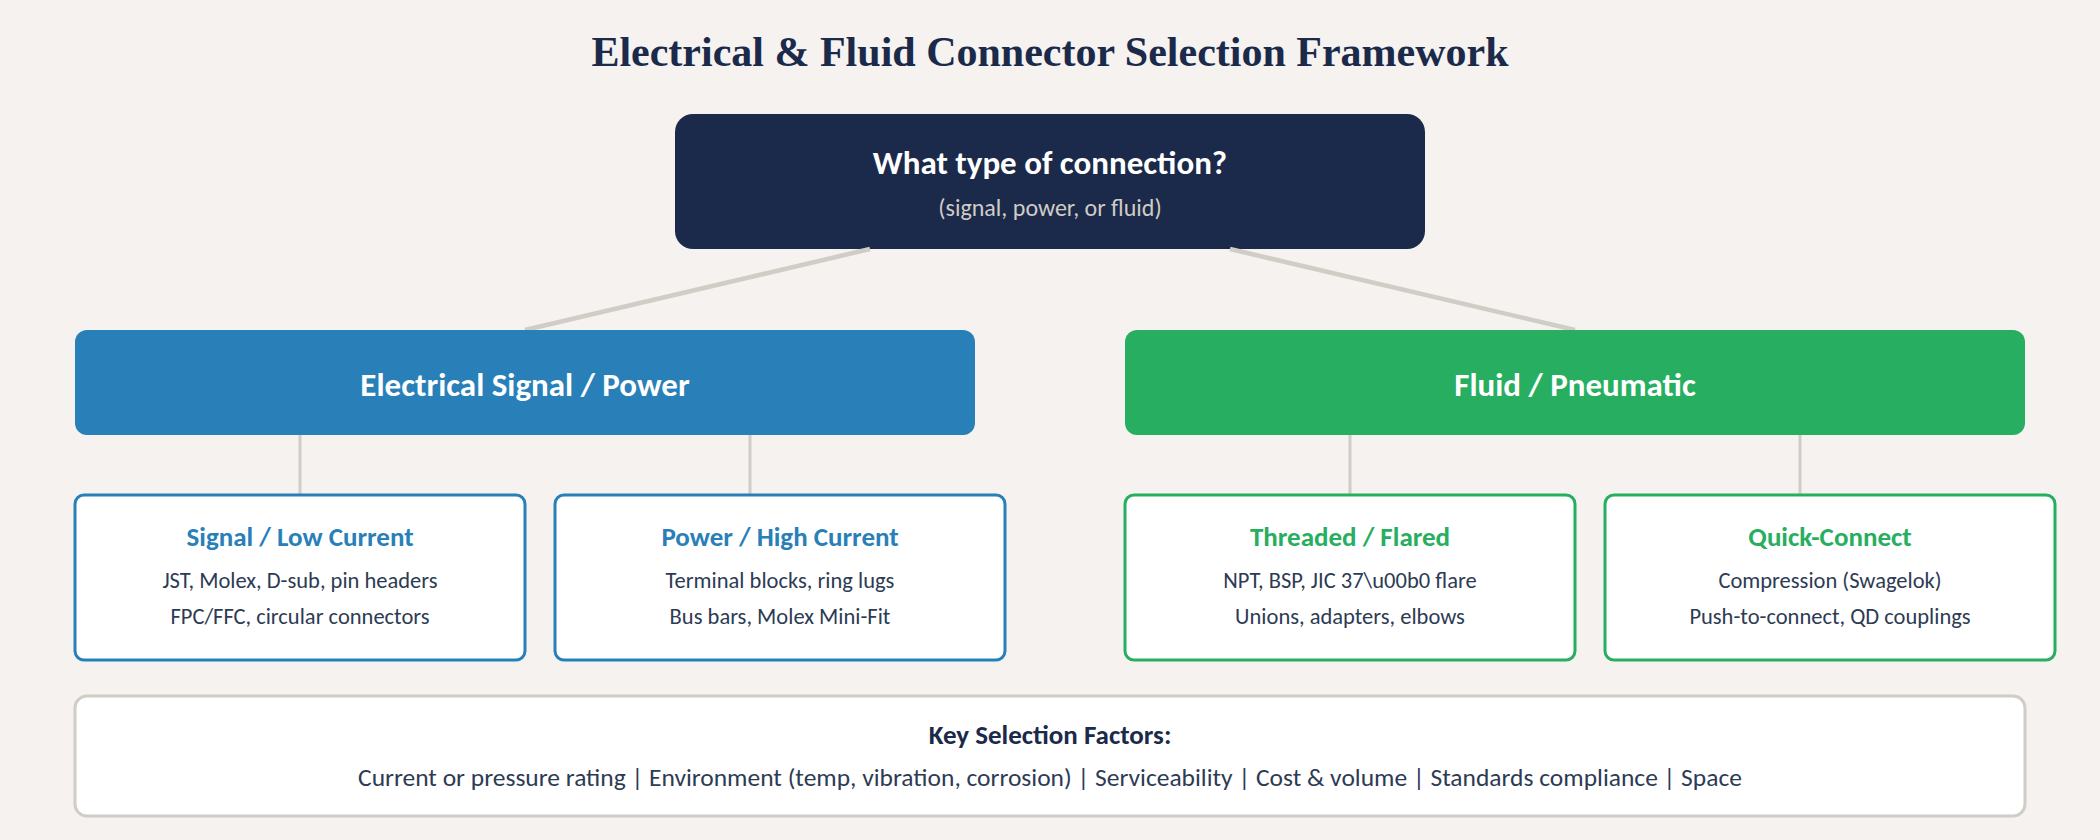
\includegraphics[width=\textwidth]{master_figs/fig4_selection_framework.png}
\caption{Decision tree for electrical and fluid connector selection.}
\label{fig:selection_framework}
\end{figure}

\begin{tipbox}[Spec the Connector First]
The connector determines wire gauge, tube OD, termination tooling, and housing envelope. Select the connector family first (based on rating, environment, and serviceability), then design the wiring or tubing around it, not the other way around.
\end{tipbox}

\subsection{Design Rules of Thumb}

\begin{enumerate}[leftmargin=1.5em]
  \item \textbf{Derate everything.} Never operate at 100\% of rated current, pressure, or temperature. A 25\% safety margin is minimum engineering practice; 50\% is professional practice for critical systems.

  \item \textbf{Design for Assembly (DFA).} Provide wrench clearance around fittings. Group fluid connections for leak-test access. Use consistent connector families within a subsystem to reduce tool count and spare parts inventory.

  \item \textbf{For fluid systems}: Verify thread standard with a gauge before assembly. Use manufacturer torque specifications. Pressure-test every joint before commissioning; hydrostatic test at $1.5\times$ working pressure per ASME B31.3~[8].

  \item \textbf{For electrical systems}: Pull-test a sample of crimps per IPC/WHMA-A-620. Verify contact resistance with a milliohm meter. Document every connector in your wire harness schedule.

  \item \textbf{Document every choice.} Record part number, manufacturer, specifications, and selection rationale in your Bill of Materials (BOM). Your future self and your teammates will need this information for procurement, assembly, and troubleshooting.
\end{enumerate}


\subsection{Key Standards Reference}

\begin{longtable}{l l p{7.5cm}}
  \toprule
  \textbf{Standard} & \textbf{Org} & \textbf{Scope} \\
  \midrule
  \endfirsthead
  \toprule
  \textbf{Standard} & \textbf{Org} & \textbf{Scope} \\
  \midrule
  \endhead
  IEC 61984~[2] & IEC & Electrical connector safety requirements, testing, and performance criteria \\
  IEC 60529~[3] & IEC & IP ingress protection rating system (IP67, IP68, IP69K) \\
  MIL-DTL-38999~[4] & U.S.\ DoD & Military circular connectors for high-performance, harsh-environment applications \\
  UL 486A-486B & UL & Safety certification for wire connectors: crimp, solder, and IDC terminations \\
  SAE J514~[5] & SAE & JIC 37$^{\circ}$\ flare hydraulic tube fittings; dimensions and performance requirements \\
  ASME B1.20.1~[6] & ASME & NPT tapered pipe thread form, dimensions, and tolerances \\
  ISO 228 / ISO 7-1~[7] & ISO & BSP parallel (BSPP) and tapered (BSPT) pipe thread standards \\
  ASME B31.3~[8] & ASME & Process piping code; materials, fabrication, inspection, and testing \\
  \bottomrule
\end{longtable}


% ══════════════════════════════════════════════════════════════════════
\section{Applying Connectors in Your Design Projects}
% ══════════════════════════════════════════════════════════════════════

Incorrect connector selection is one of the most common failure modes in student design projects. The following workflow ensures systematic coverage.

\begin{enumerate}[leftmargin=1.5em]
  \item \textbf{Create a connection schedule early.} List every electrical and fluid joint in your design. Classify each by type (wire-to-wire, wire-to-board, NPT, JIC, etc.). This becomes a living document through your design reviews.

  \item \textbf{For every electrical connection, specify}: connector family, pin count, current rating (derated), voltage rating, IP rating, termination method, wire gauge, and mating cycles.

  \item \textbf{For every fluid connection, specify}: fitting standard (NPT, BSP, JIC, or compression), nominal size, working pressure, seal material, fluid compatibility, and assembly torque.

  \item \textbf{Build a complete BOM} with manufacturer part numbers and procurement sources. Recommended suppliers:
  \begin{itemize}[nosep]
    \item Electrical: Digi-Key, Mouser, Newark, Allied.
    \item Fluid: Swagelok, Parker, McMaster-Carr, Grainger.
  \end{itemize}

  \item \textbf{Design review milestones}:
  \begin{itemize}[nosep]
    \item \textbf{PDR}: Present your connection schedule.
    \item \textbf{CDR}: Present datasheets and torque specifications.
    \item \textbf{FDR}: Demonstrate assembly procedures and test results.
  \end{itemize}

  \item \textbf{Test every connection before commissioning}: Pull-test electrical crimps, measure contact resistance with a milliohm meter, and pressure-test all fluid joints at $1.5\times$ working pressure.
\end{enumerate}


% ══════════════════════════════════════════════════════════════════════
\section{Quick-Reference Summary}
% ══════════════════════════════════════════════════════════════════════

\begin{keyconceptbox}[Five Key Takeaways]
\begin{enumerate}[nosep,leftmargin=1.5em]
  \item Electrical connectors are classified by \emph{what they connect} (wire-to-wire, wire-to-board, board-to-board) and \emph{how they terminate} (crimp, solder, IDC, screw, press-fit).
  \item For every electrical connection, specify: current rating, voltage rating, IP rating, contact resistance, and mating cycles, and derate for temperature.
  \item Fluid connectors require matching thread standards. NPT $\neq$ BSP. JIC 37$^{\circ}$\ flare and compression fittings avoid the pitfalls of tapered-thread sealing.
  \item Failure modes differ by domain: electrical joints fail from fretting corrosion and $I^2R$ overheating; fluid joints fail from cross-threading and seal degradation.
  \item Every connector specification follows the same logic: \textbf{rating $\to$ environment $\to$ serviceability $\to$ cost $\to$ standards $\to$ space}. Document everything in your BOM.
\end{enumerate}
\end{keyconceptbox}


% ══════════════════════════════════════════════════════════════════════
\section{Artifact Handoff: What This Chapter Supports}
\begin{table}[htbp]\centering\small
\begin{tabularx}{\textwidth}{l X l}
\toprule
\textbf{Artifact} & \textbf{Description} & \textbf{Forward Reference} \\
\midrule
Connector Specifications & Selected connectors with ratings in BOM & Ch.~5 (ICDs) \\
Wire/Tube Routing & Harness design and fluid line layout & Assembly drawings \\
\bottomrule
\end{tabularx}
\end{table}


\begin{keyconceptbox}[Requirements Mapping: From Connector Specs to Shall-Statements]
Connector specifications generate system requirements:
\begin{itemize}[nosep,leftmargin=1.5em]
\item ``Outdoor deployment in rain'' $\to$ SYS-REQ: All external connectors shall be rated IP67 or higher.
\item ``Field-replaceable sensor'' $\to$ SYS-REQ: Sensor connections shall use keyed, tool-free connectors rated for $\geq$100 mating cycles.
\item ``Motor draws 8\,A continuous'' $\to$ CONN-REQ: Motor power connectors shall be rated for $\geq$10\,A continuous (20\% margin) with 12\,AWG wire termination.
\item ``Hydraulic test pressure 200\,psi'' $\to$ CONN-REQ: All fluid fittings shall be rated for $\geq$800\,psi working pressure ($4\times$ safety factor per hydraulic standard).
\end{itemize}
Every connector in your BOM must trace to a requirement. If you cannot write a shall-statement for it, you have not justified the selection.
\end{keyconceptbox}

\section{Practice Questions for Quiz Preparation}
% ══════════════════════════════════════════════════════════════════════

Use these questions to test your understanding. Answers follow on the next page.

\subsection{Conceptual Questions}

\begin{enumerate}[leftmargin=1.5em]
  \item What are the three fundamental elements of every electrical connector?

  \item A connector is rated at 15\,A per contact at 25\,\degC{}. Your design has an ambient temperature of 75\,\degC{} and all 12 contacts are loaded. Why should you \emph{not} assume 15\,A per contact is safe?

  \item Explain why fretting corrosion is considered the ``most insidious'' electrical connector failure mode.

  \item You need to connect a hydraulic line rated at 5000\,psi that will be disconnected for maintenance monthly. Which fitting family is most appropriate? Why?

  \item A colleague suggests using PTFE tape on a BSPP fitting. Is this correct? Explain.

  \item What is the difference between rated working voltage and dielectric withstand voltage? Which should appear in your design documentation?

  \item Why does NPS (Nominal Pipe Size) create confusion when specifying fittings?

  \item Describe two mitigations for vibration fatigue in fluid tubing systems.

  \item You measure 50\,m$\Omega$ contact resistance on a connector carrying 8\,A. How much power is dissipated as heat at that contact? Is this a concern?

  \item Compare the sealing mechanisms of NPT, JIC 37$^{\circ}$\ flare, and compression fittings. Which requires sealant?
\end{enumerate}

\subsection{Application / Scenario Questions}

\begin{enumerate}[resume,leftmargin=1.5em]
  \item Your design team is designing an outdoor weather station. You need a 6-pin connector for sensor signals (all under 500\,mA) that will be installed once and never disconnected. What IP rating, plating, and mating-cycle specification would you select? Justify your choices.

  \item A pneumatic system in your project uses 1/4\,in.\ OD nylon tubing at 80\,psi. Recommend a fitting type and explain why.

  \item Your design uses both NPT and BSP components (sourced from U.S.\ and European manufacturers). What steps must you take to ensure safe assembly?

  \item You are specifying connectors for a cooling loop carrying a 50/50 ethylene glycol--water mix at 200\,$^{\circ}$F and 50\,psi. What seal material would you select? What body material?

  \item At your CDR, a reviewer asks: ``How did you verify your crimp terminations are reliable?'' Describe the test procedure you would reference.

  \item \textbf{Diagnostic scenario}: Your team's prototype passes a low-voltage continuity check on the bench (all connections show $<$1\,$\Omega$), but the system experiences intermittent sensor dropouts and a motor controller that occasionally faults when the prototype is running on a vibration table or driving over rough terrain. Where do you start your investigation, and what failure modes should you suspect? Describe the diagnostic steps you would take, referencing at least three concepts from this module.
\end{enumerate}


\newpage
\subsection{Answers}

\begin{enumerate}[leftmargin=1.5em]
  \item Contacts (conductive pins/sockets), housing (insulating body), and termination (wire-to-contact joint).

  \item Two derating effects compound: (a) elevated ambient temperature reduces the thermal headroom of the housing, and (b) thermal stacking from all 12 contacts being loaded raises the internal housing temperature further. The manufacturer's derating curve must be consulted; actual safe current per contact could be as low as 10\,A or less.

  \item Fretting corrosion develops slowly from micro-vibration, manifests as intermittent (not permanent) high resistance, is invisible without disassembly, and is difficult to reproduce during troubleshooting. By the time symptoms are consistent, oxide debris has accumulated extensively.

  \item JIC 37$^{\circ}$\ flare (SAE J514). It handles 10000\,psi (well above 5000\,psi), provides a metal-to-metal seal that doesn't degrade with reassembly, and is designed for repeated disconnect/reconnect without special tools beyond standard wrenches. Compression would also work but ferrules deform on initial assembly, making reassembly less reliable.

  \item Incorrect. BSPP (G-type) uses parallel threads that do \emph{not} seal on the threads. Sealing is achieved with a bonded washer or O-ring against a flat face. PTFE tape is used on \emph{tapered} threads (NPT, BSPT) where the thread interference provides the primary seal. Applying tape to BSPP serves no useful purpose and may prevent proper washer compression.

  \item Working voltage is the maximum voltage at which the connector is rated for continuous, safe operation, including creepage and clearance margins per IEC 61984. Dielectric withstand (breakdown) voltage is the voltage at which insulation fails; it is a destructive test limit, not an operating specification. Always specify working voltage in design documentation.

  \item NPS is a nominal designation, not a physical dimension. For example, 1/2\,in.\ NPS has an OD of 0.840\,in. Engineers unfamiliar with this convention may attempt to match fittings by measuring OD, leading to incorrect specifications. Always reference the NPS table and verify with thread gauges.

  \item (a) Install tube support clamps at manufacturer-recommended intervals to eliminate unsupported spans. (b) Include flexible hose segments at vibration sources (pumps, engines) to decouple cyclic motion from rigid tubing.

  \item $P = I^2R = (8)^2 \times 0.050 = 3.2\,W$. Yes, this is a concern; 3.2\,W of localized heat will raise the contact and housing temperature significantly. This level of contact resistance suggests degraded contacts that should be inspected and potentially replaced.

  \item NPT: Thread interference creates a wedge seal, but clearance at crests/roots requires supplemental sealant (PTFE tape or pipe dope). JIC 37$^{\circ}$: Metal-to-metal cone seal at the flared tube end; no sealant required. Compression: Ferrule swaged onto tube OD creates the seal mechanically; no sealant required. Only NPT (and BSPT) requires sealant.

  \item IP67 (dust-tight, survives 1\,m immersion for rain/flooding protection). Gold plating (resists corrosion in outdoor environment with humidity and temperature cycling). 25--50 mating cycles (permanent installation, only disconnected for rare maintenance). Lower mating cycle connectors are less expensive and can be more robust.

  \item Push-to-connect fittings. At 80\,psi with nylon tubing, this is well within the 250\,psi range of push-to-connect. Benefits: tool-free assembly, compatible with nylon tubing, easy reconfiguration, and widely available in 1/4\,in.\ OD size from SMC, Festo, or John Guest.

  \item (a) Create a thread identification chart for the project listing which ports are NPT and which are BSP. (b) Verify every connection with a thread pitch gauge (\ang{60} = NPT, \ang{55} = BSP) before assembly. (c) If adaptation is needed, use NPT-to-BSP adapter fittings from a reputable manufacturer. Never force-thread. (d) Label all ports on your assembly drawings with thread standard.

  \item Seal: Viton (FKM); compatible with ethylene glycol, rated to 400\,$^{\circ}$F (above the 200\,$^{\circ}$F operating temperature). Body: stainless steel or brass (both compatible with glycol--water). Avoid carbon steel unless corrosion-protected, as glycol solutions can be mildly corrosive to unprotected ferrous metals.

  \item Reference IPC/WHMA-A-620 standard. Procedure: (a) Pull-test a statistical sample of crimps at the specified force for the wire gauge and contact size. (b) Cross-section a sample crimp to verify the cold-weld zone under magnification. (c) Measure contact resistance across each mated pair with a milliohm meter; verify $<$20\,m$\Omega$ for gold-plated contacts. (d) Document results with crimp force values, pass/fail criteria, and inspector sign-off.

  \item This scenario synthesizes three interconnected failure modes. \textbf{Primary suspect: fretting corrosion.} The hallmark is a system that passes static bench testing but fails under dynamic load, exactly the intermittent, vibration-dependent behavior described in the fretting progression (Section~\ref{sec:elecfailure}, Figure~\ref{fig:fretting_progression}). Diagnostic steps: (a)~Measure contact resistance across every mated connector pair with a milliohm meter \emph{while the system is subject to vibration} (tap on connectors, flex cables). Resistance that fluctuates from milliohms to ohms on disturbance confirms fretting. (b)~Check for $I^2R$ heating: use a thermal camera to identify hot connectors under load. A connector running 10\,A through a fretting contact at 500\,m$\Omega$ dissipates 5\,W, enough to soften a nylon housing. (c)~Inspect strain relief: if cables transmit vehicle vibration directly to the contact zone, fretting is accelerated regardless of plating. (d)~Check connector specifications: are tin-plated contacts being used in a high-vibration application where gold plating is warranted? Is the contact normal force sufficient? (e)~For the motor controller faults specifically, consider whether the power connector is derated for the actual ambient temperature inside the enclosure under operation. Resolution: replace affected contacts with gold-plated equivalents, add proper strain-relief clamps, install secondary locking features (CPA clips), and retest under dynamic load with milliohm monitoring.
\end{enumerate}


% ══════════════════════════════════════════════════════════════════════


\subsection{Application Scenario Answers}
\begin{enumerate}[leftmargin=1.5em, start=11]
\item \textbf{Redesigning a student project from soldered connections to connectors}:

\textbf{Step 1}: Identify every wire-to-wire and wire-to-board connection in the system. Create a connection table: source, destination, signal type (power/signal/data), current, voltage, mating cycles expected.

\textbf{Step 2}: Group connections by subsystem boundary. Each subsystem-to-subsystem boundary gets one multi-pin connector (e.g., sensor module connects to controller via one 4-pin JST-XH: VCC, GND, SDA, SCL).

\textbf{Step 3}: Select connector families. For low-current signals ($<$1\,A): JST-XH (wire-to-board, 2.5\,mm pitch, rated 3\,A, keyed). For power ($>$1\,A): XT30 (rated 30\,A, gendered, compact) or Anderson Powerpole (genderless, stackable). For board-to-board: standard 2.54\,mm pin headers with locking housings.

\textbf{Step 4}: Create a wiring diagram showing every connector with pin assignments, wire colors, and wire gauges. This diagram is a CDR deliverable.

\textbf{Step 5}: Label every connector pair with matching alphanumeric codes (J1/P1, J2/P2, etc.) on both the connector and the wiring diagram.

Benefits: any subsystem can be disconnected, tested independently, and reconnected. Failed modules can be swapped without soldering. The system can be disassembled for transport and reassembled on-site.
\end{enumerate}

\chapter{Power Supplies, Motors \& Pumps}

\vspace{1em}




\vspace{1em}

% ══════════════════════════════════════════════════════════════════════
\section{Power Supply Selection}
% ══════════════════════════════════════════════════════════════════════

\subsection{What a Power Supply Does}

A power supply converts electrical energy from a source, AC mains, battery, solar panel, or USB, into one or more regulated DC voltage rails that your circuits and actuators require. Every component in your design has a specific voltage and current requirement. A typical student project might need 3.3\,V for the microcontroller, 5\,V for sensors and logic, and 12\,V or 24\,V for motors and solenoids. The power supply must deliver all of these simultaneously with adequate regulation and current capacity.

\subsection{Linear Regulators (LDO)}

Linear regulators are the simplest power supply topology. They are essentially a controllable series resistance that drops the input voltage to the desired output, dissipating the excess as heat.

\begin{equation}
  P_{\text{waste}} = (V_{\text{in}} - V_{\text{out}}) \times I_{\text{load}}, \qquad \eta = \frac{V_{\text{out}}}{V_{\text{in}}} \times 100\%
\end{equation}

An LM7805 producing 5\,V from 12\,V at 1\,A wastes 7\,W as heat with only 42\% efficiency. A low-dropout (LDO) regulator reduces the minimum input-to-output voltage difference to as little as 200\,mV, improving efficiency when the differential is small.

\begin{tipbox}[When to Use an LDO]
Use LDOs when: (1) the voltage drop is small ($<2\,V$), (2) current is under $\$\sim\$$1\,A, (3) noise matters (analog sensors, audio, ADCs), or (4) simplicity matters (only 2 capacitors, no inductor needed). Common devices: LM7805 (5\,V/1\,A), AMS1117-3.3 (3.3\,V/1\,A), MCP1700 (3.3\,V/250\,mA, ultra-low quiescent current).
\end{tipbox}

\subsection{Switching Regulators (DC-DC Converters)}

Switching regulators chop the input voltage at high frequency (100\,kHz--2\,MHz) and use an inductor to transfer energy efficiently, achieving 85--95\% efficiency.

\subsubsection{Buck (Step-Down): $V_{\text{out}} < V_{\text{in}}$}

The workhorse of DC-DC conversion. A switching FET, inductor, and capacitor step voltage down. Typical efficiency 85--95\%. Common devices: LM2596 (3\,A), MP1584 (3\,A), TPS54302 (3\,A). Pre-built module boards are available for under \$2; recommended for student projects because the critical PCB layout is already done.

\textbf{Example}: 12\,V battery $\to$ 5\,V at 2\,A. At 90\% efficiency, waste heat is only 1.1\,W compared to 14\,W for a linear regulator.

\subsubsection{Boost (Step-Up): $V_{\text{out}} > V_{\text{in}}$}

Stores energy in an inductor during the switch-on phase, then releases it at higher voltage during switch-off. Typical efficiency 80--93\%. Common devices: MT3608 (2\,A), TPS61088 (10\,A). Important limitation: most boost converters cannot fully disconnect the load from the input.

\subsubsection{Buck-Boost: $V_{\text{out}} \gtrless V_{\text{in}}$}

Handles input voltage that swings above and below the output; essential for battery applications. A LiPo cell ranges from 4.2\,V (full) to 3.0\,V (depleted). If your circuit needs 3.3\,V, the input crosses the output during discharge. Only buck-boost works through this transition. Common: TPS63020 (3.6\,A), LTC3780.

\begin{warningbox}[EMI from Switching Regulators]
All switching regulators generate electromagnetic interference at their switching frequency. This can corrupt ADC readings, cause radio interference, and inject noise into audio circuits. Always follow the datasheet layout recommendations: keep switching traces short, use a continuous ground plane, and place input/output capacitors as close to the regulator as physically possible. When powering noise-sensitive circuits, add an LDO downstream of the switcher as a noise filter.
\end{warningbox}

\subsection{AC-DC Power Supplies}

For systems that plug into AC mains (120/240\,VAC), you need an AC-to-DC conversion stage with galvanic isolation to separate lethal mains voltage from safe low-voltage outputs.

\begin{warningbox}[Student Project Rule]
\textbf{Never design your own AC-DC converter.} Always use a pre-certified wall adapter (UL/CE listed) that provides a regulated DC output. These are fully enclosed, safety-certified, and eliminate all mains-voltage hazards from your design. If a wall adapter cannot meet your requirements, use an enclosed industrial supply (Mean Well, TDK-Lambda) with proper enclosure design.
\end{warningbox}


\begin{warningbox}[LiPo Battery Safety: This Is Not Optional]
A lithium-polymer battery that is overcharged, over-discharged, punctured, or short-circuited can undergo thermal runaway: \textbf{fire and toxic gas release} within seconds. A LiPo fire in a campus lab is a safety emergency that can end careers and close facilities. \textbf{Mandatory rules for MEGN~301}:
\begin{itemize}[nosep,leftmargin=1.5em]
\item \textbf{Never} charge a LiPo without a functional Battery Management System (BMS) with cell-level overvoltage, undervoltage, and overcurrent protection.
\item \textbf{Never} leave a charging LiPo unattended.
\item \textbf{Always} charge and store LiPo batteries in a fireproof LiPo safety bag.
\item \textbf{Never} use a battery with a puffy or swollen pouch; it is generating gas internally.
\item Violation of these rules is grounds for immediate lab access revocation.
\end{itemize}
\end{warningbox}

\subsection{Key Power Supply Specifications}
\label{sec:psu_specs}

\begin{table}[htbp]
\centering\small
\begin{tabularx}{\textwidth}{l X}
  \toprule
  \textbf{Specification} & \textbf{Description} \\
  \midrule
  Output Voltage & Nominal output with tolerance (e.g., 5.0\,V $\pm$2\%). Must match each load rail. \\
  Output Current & Max continuous delivery. Must exceed total load current with $\geq$20\% margin. \\
  Regulation & Line regulation: output change when input varies. Load regulation: output change when load varies. Expressed as \% or mV. \\
  Ripple \& Noise & Peak-to-peak AC on the DC output. Switchers: 20--100\,mV. LDOs: $<$1\,mV. \\
  Efficiency & $P_{\text{out}} / P_{\text{in}} \times 100\%$. LDO: 40--80\%. Buck: 85--95\%. Determines waste heat and battery life. \\
  Isolation \& Safety & Galvanic isolation for AC-DC. Look for UL/CSA/CE marks. \\
  \bottomrule
\end{tabularx}
\caption{Key power supply specifications.}
\end{table}

\subsection{Power Supply Failure Modes}

\begin{itemize}[leftmargin=1.5em]
  \item \textbf{Overcurrent}: Motor inrush can be 6--10$\times$ running current. Size for peak, not average.
  \item \textbf{Thermal failure}: Every supply has a derating curve; output current decreases with ambient temperature.
  \item \textbf{Input transients}: Voltage spikes from motor switching. Mitigate with input capacitors and TVS diodes.
  \item \textbf{Capacitor aging}: Electrolytic caps dry out, increasing ripple. Use 105\,\degC{} rated caps.
\end{itemize}


\begin{figure}[htbp]
\centering
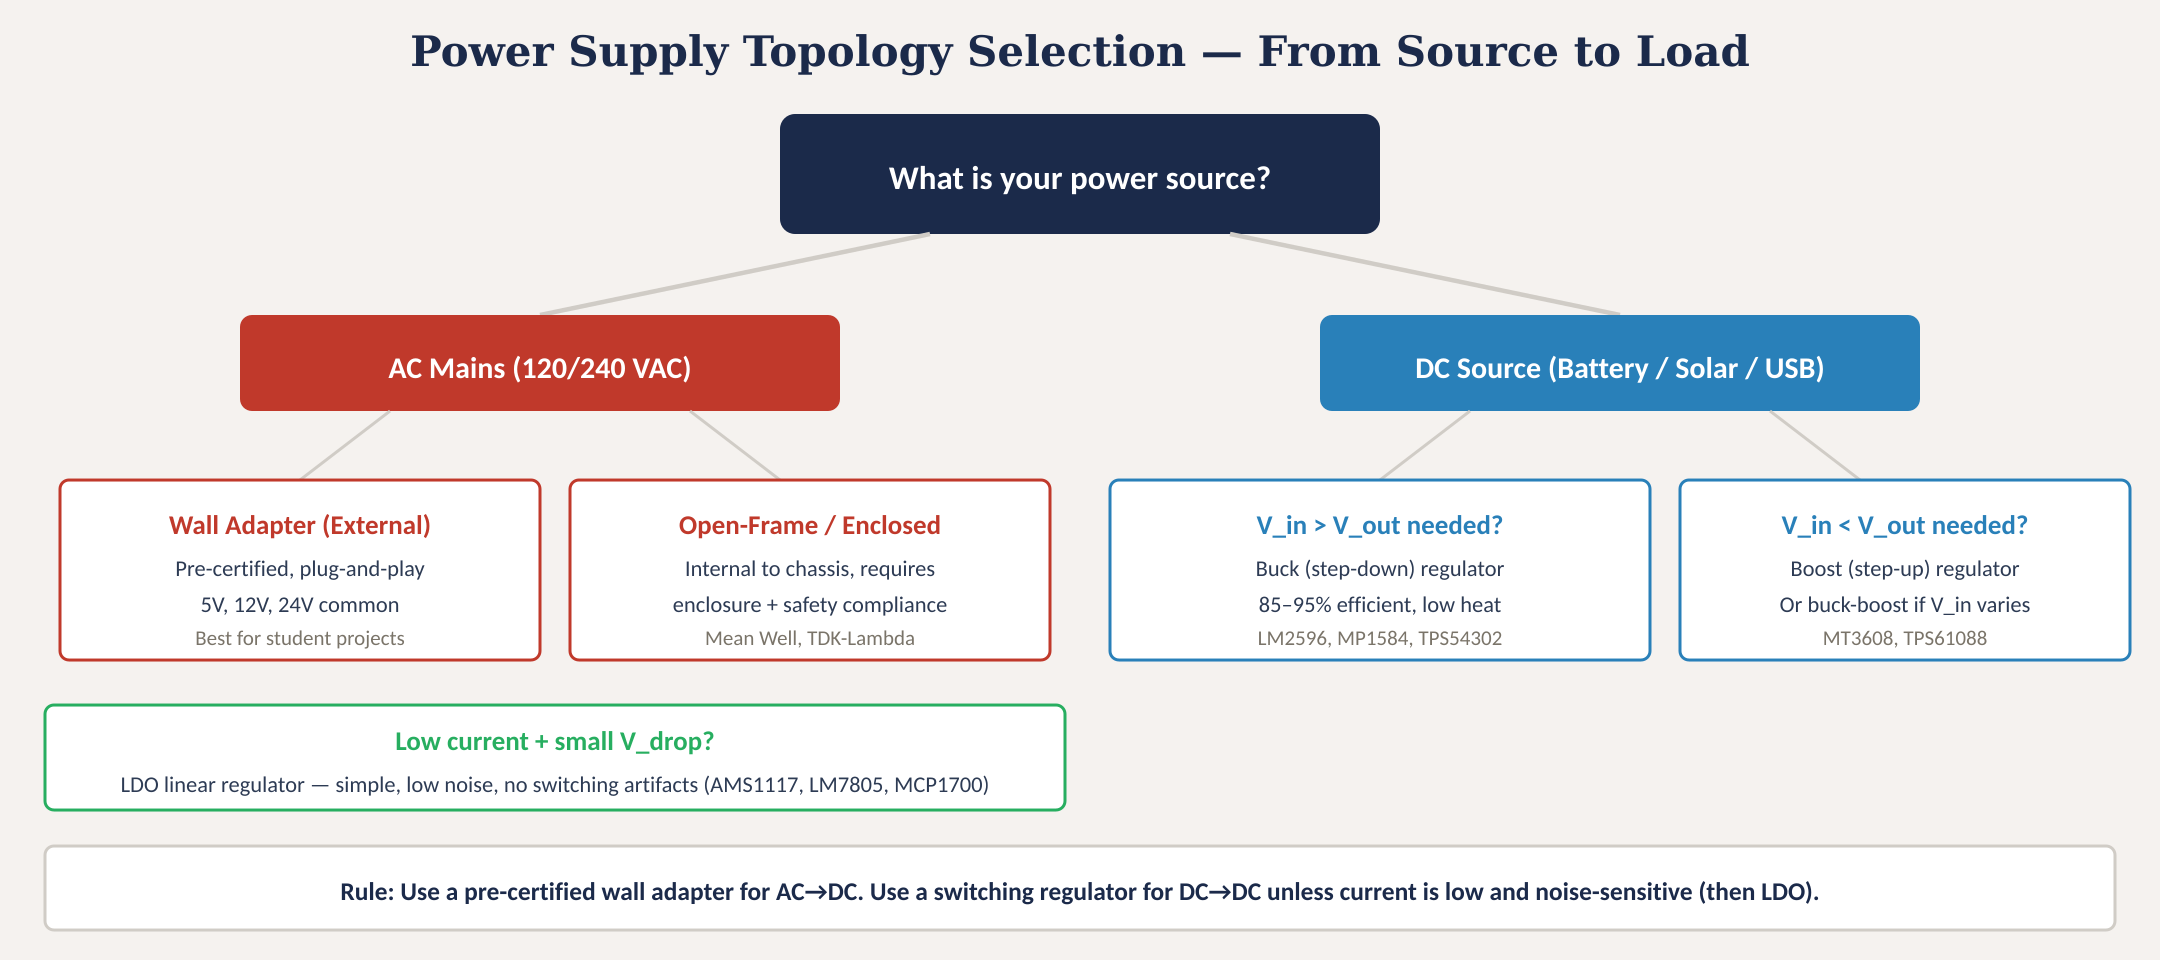
\includegraphics[width=\textwidth]{master_figs/fig_psu_topology.png}
\caption{Power supply topology decision tree, from source type through voltage conversion to specific regulator selection.}
\label{fig:psu_topology}
\end{figure}


% ══════════════════════════════════════════════════════════════════════
\section{DC Motors}
% ══════════════════════════════════════════════════════════════════════

\subsection{Motor Fundamentals}

Every DC motor operates on the Lorentz force: a current-carrying conductor in a magnetic field experiences a force. Two equations govern motor behavior:

\begin{align}
  \tau &= K_t \times I \quad \text{(torque is proportional to current)} \\
  V_{\text{back-EMF}} &= K_e \times \omega \quad \text{(back-EMF is proportional to speed)}
\end{align}

At stall ($\omega = 0$), back-EMF is zero and current is limited only by winding resistance: $I_{\text{stall}} = V / R_{\text{winding}}$. This is typically 6--10$\times$ the rated running current and causes rapid overheating.

\subsection{Brushed DC Motors}

Simplest motor type. Mechanical commutation via carbon brushes on a copper commutator. Apply voltage, it spins; reverse polarity, it reverses. Speed control via PWM. The torque-speed curve is linear from stall torque at zero speed to no-load speed at zero torque.

\textbf{Advantages}: Cheap, simple to drive (just PWM + H-bridge), widely available.

\textbf{Limitations}: Brush wear limits lifetime (1,000--5,000 hours), EMI from brush arcing, moderate efficiency (70--85\%).

\subsection{Brushless DC (BLDC) Motors}

Permanent magnets on the rotor, three-phase windings on the stator. An Electronic Speed Controller (ESC) sequentially energizes the stator phases. The motor \emph{cannot function without its ESC}; they are an inseparable system.

\textbf{Advantages}: 85--95\% efficiency, 10,000+ hour life, higher power density, flat torque curve in the mid-range, lower EMI.

\textbf{Limitations}: Requires ESC (adds cost and complexity), cannot be driven directly from DC, commutation tuning matters.

\subsection{Stepper Motors}

Rotate in discrete angular steps (typically \ang{1.8} = 200 steps/rev). Open-loop positioning: count steps to know position without an encoder. NEMA 17 is the standard frame size for student projects. Driver boards (A4988, TMC2209) accept step/direction signals from any microcontroller.

\textbf{Advantages}: Precise positioning, high holding torque, no encoder needed.

\textbf{Limitations}: Torque drops rapidly with speed, runs hot (always energized), skips steps silently under overload.

\subsection{Servo Motors}

A motor + encoder + controller in a closed-loop system. Hobby servos (SG90, MG996R) are self-contained with PWM control. Industrial servos use BLDC motors with high-resolution encoders and dedicated controllers running PID loops at kHz rates.

\begin{figure}[htbp]
\centering
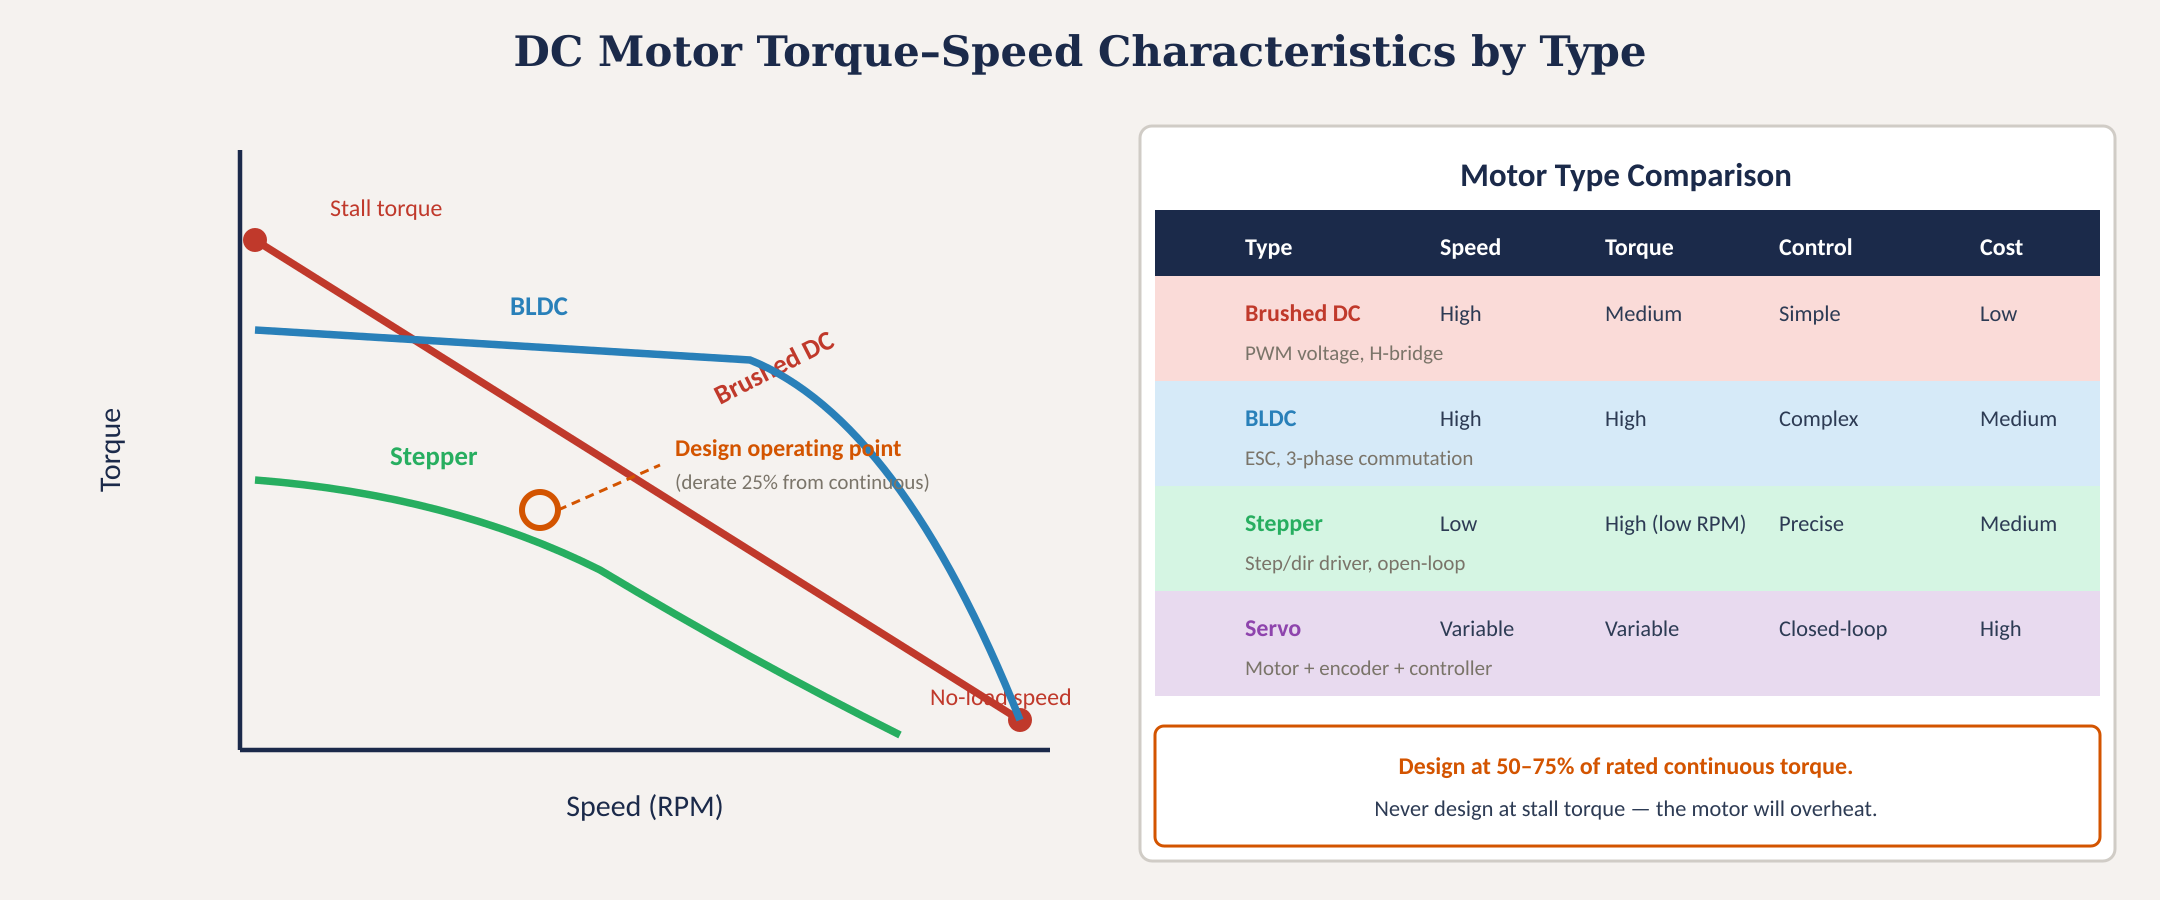
\includegraphics[width=\textwidth]{master_figs/fig_motor_curves.png}
\caption{Torque--speed characteristics for brushed DC (linear), BLDC (flat mid-range), and stepper (high-torque at low RPM) with comparison table.}
\label{fig:motor_curves}
\end{figure}

\subsection{Key Motor Specifications}

\begin{table}[htbp]
\centering\small
\begin{tabularx}{\textwidth}{l X}
  \toprule
  \textbf{Specification} & \textbf{Description} \\
  \midrule
  Rated Voltage & Nominal operating voltage. Must match your supply rail. \\
  No-Load Speed & Max speed with no load (RPM). Actual speed under load is lower. \\
  Stall Torque & Max torque at zero speed. \textbf{NOT your design point}; stall current overheats the motor. \\
  Rated / Continuous Torque & Torque the motor delivers indefinitely. Your design ceiling. Derate to 50--75\%. \\
  Rated Current & Current at rated torque. Sizes your driver and power supply. \\
  Torque Constant ($K_t$) & Torque per ampere (N$\cdot$m/A). Calculate required current: $I = \tau_{\text{load}} / K_t$. \\
  \bottomrule
\end{tabularx}
\caption{Key motor specifications.}
\end{table}

\begin{warningbox}[Never Design at Stall Torque]
Stall current = $V_{\text{rated}} / R_{\text{winding}}$, typically 6--10$\times$ the rated running current. At stall, all electrical power converts to heat in the windings. A motor will overheat and fail within seconds to minutes. Always design at 50--75\% of the \emph{continuous} rated torque.
\end{warningbox}

\subsection{Motor Drive Electronics}
\label{sec:motor_drivers}

Every motor type needs a matched driver circuit:

\begin{itemize}[leftmargin=1.5em]
  \item \textbf{H-Bridge (Brushed DC)}: Four transistors for bidirectional current. L298N (2A, legacy), BTS7960 (43A), DRV8871 (3.6A). \textbf{Must include flyback diodes}; back-EMF from inductive loads will destroy unprotected transistors.
  \item \textbf{ESC (BLDC)}: Converts DC + throttle signal to three-phase AC. Drone ESCs are cheap and widely available. Use bidirectional or 4-quadrant ESC for reversing.
  \item \textbf{Stepper Driver}: Converts step + direction signals into motor phase currents. A4988 (2A), DRV8825 (2.5A), TMC2209 (2A, silent). \textbf{Set the current limit potentiometer before powering on.}
  \item \textbf{Servo Controller}: Hobby servos need only a PWM signal (1--2\,ms pulse, 50\,Hz). Industrial servos require dedicated controllers.
\end{itemize}


% ══════════════════════════════════════════════════════════════════════
\section{Pumps}
% ══════════════════════════════════════════════════════════════════════

\subsection{Positive Displacement vs.\ Dynamic}

\textbf{Positive displacement (PD)} pumps trap a fixed volume per cycle and force it into the discharge. Flow is proportional to speed and nearly independent of pressure. Self-priming. Pulsating flow. Types: gear, diaphragm, peristaltic, piston, vane.

\textbf{Dynamic (centrifugal)} pumps impart kinetic energy to the fluid via a spinning impeller. Flow varies with discharge pressure (follows a pump curve). Smooth, continuous flow. \emph{Not} self-priming. Best for high-volume, lower-pressure applications.

\subsection{Pump Types}

\subsubsection{Gear Pumps}
Two meshing gears trap fluid between teeth and housing. Self-priming, handles viscous fluids (oil, glycol). Constant flow rate. Used in hydraulic systems and lubrication. Primary failure mode: wear from particle contamination. Always use inline filtration.

\subsubsection{Diaphragm Pumps}
A flexible diaphragm oscillates to create suction and discharge. Seal-less design isolates fluid from moving parts. Self-priming, handles corrosive and abrasive fluids. Pulsating flow requires dampeners.

\subsubsection{Peristaltic Pumps}
Rollers compress a flexible tube, pushing fluid forward. Zero contamination risk; fluid only contacts the tube. Easy maintenance: swap the tube. Gentle on shear-sensitive fluids. Limited to $\$\sim\$$30\,psi. Tube fatigue is the primary maintenance concern.

\subsubsection{Centrifugal / Impeller Pumps}
Spinning impeller accelerates fluid radially. Smooth, high-volume flow. Requires flooded suction (not self-priming). Poor with viscous fluids. Small 12V DC impeller pumps are widely available for student cooling and circulation projects.

\begin{figure}[htbp]
\centering
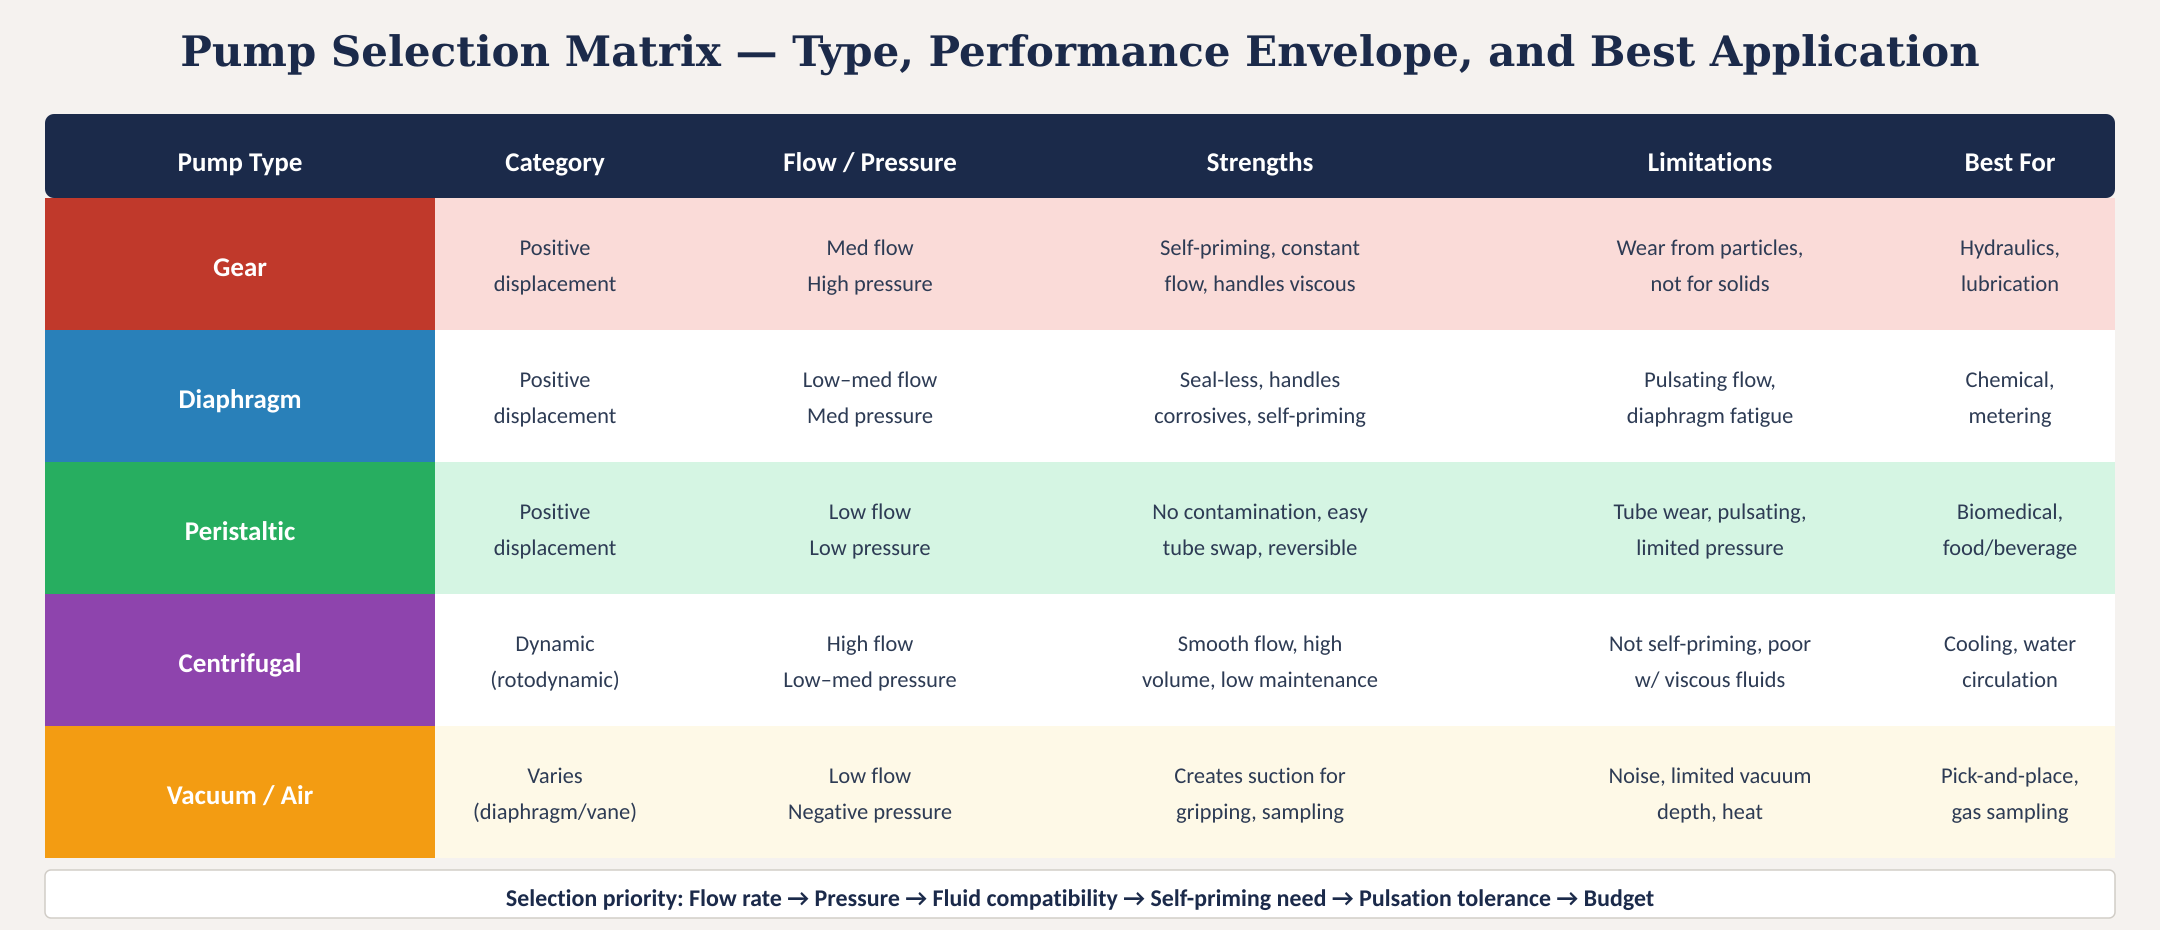
\includegraphics[width=\textwidth]{master_figs/fig_pump_matrix.png}
\caption{Pump selection matrix; type, performance envelope, strengths, limitations, and best applications.}
\label{fig:pump_matrix}
\end{figure}

\subsection{Key Pump Specifications}

\begin{table}[htbp]
\centering\small
\begin{tabularx}{\textwidth}{l X}
  \toprule
  \textbf{Specification} & \textbf{Description} \\
  \midrule
  Flow Rate & Volume per unit time (L/min, mL/min). Must meet demand with $\geq$25\% margin. \\
  Discharge Pressure / Head & Max pressure (psi/bar) or total dynamic head (ft/m). Must exceed system losses. \\
  Fluid Compatibility & Wetted materials must be compatible with the pumped fluid. Check seal charts. \\
  Self-Priming & PD pumps: yes. Centrifugal: no (must be flooded). \\
  Motor Integration & Many small pumps include integrated 12V/24V DC motors; specify the assembly. \\
  \bottomrule
\end{tabularx}
\caption{Key pump specifications.}
\end{table}


% ══════════════════════════════════════════════════════════════════════

\subsection{Worked Example: Motor Selection for a Belt Conveyor}

\textbf{Requirements}: Move 1\,kg payload at 0.1\,m/s on a horizontal belt conveyor. Belt drive with 50\,mm diameter driven roller.

\textbf{Step 1: Calculate load torque.}
Conveyor force = payload weight + belt friction = $(1.0 \times 9.81) + (1.0 \times 9.81 \times 0.3) = 12.75$\,N (assuming $\mu = 0.3$ for belt on roller).

Torque at roller = $F \times r = 12.75 \times 0.025 = 0.319$\,N$\cdot$m.

\textbf{Step 2: Calculate required speed.}
Roller angular velocity = $v/r = 0.1/0.025 = 4.0$\,rad/s = 38.2\,RPM.

\textbf{Step 3: Select motor with margin.}
Required motor torque (with 2$\times$ margin): $0.319 \times 2 = 0.638$\,N$\cdot$m at 38\,RPM. A typical NEMA~17 stepper (0.44\,N$\cdot$m rated) is insufficient. Options: (a) 12\,V DC gearmotor with 50:1 ratio (Pololu 37D: 0.8\,N$\cdot$m at 50\,RPM, \$25), or (b) NEMA~17 stepper with 5:1 planetary gearbox (0.44 $\times$ 5 $\times$ 0.95 = 2.09\,N$\cdot$m at 40\,RPM, \$40).

\textbf{Step 4: Verify power budget.}
$P = \tau \times \omega = 0.319 \times 4.0 = 1.28$\,W mechanical. At 70\% motor efficiency: $P_{electrical} = 1.28/0.70 = 1.83$\,W. At 12\,V: $I = 1.83/12 = 0.15$\,A running. Stall current (Pololu 37D): 5.5\,A. Power supply must handle 5.5\,A inrush.

\textbf{Step 5: Select driver.}
DC gearmotor: L298N H-bridge (2\,A continuous, inadequate for 5.5\,A stall). Better: BTS7960 (43\,A, \$8). Include flyback diodes (integrated in BTS7960).

\textbf{BOM entries}: Motor: Pololu 4756 (12V 50:1 37D gearmotor), \$24.95. Driver: BTS7960 module, \$7.50. Mounting: Pololu 1084 bracket, \$7.49.

\section{Selection and Design Practice}
% ══════════════════════════════════════════════════════════════════════

\subsection{Unified Selection Framework}

\begin{figure}[htbp]
\centering
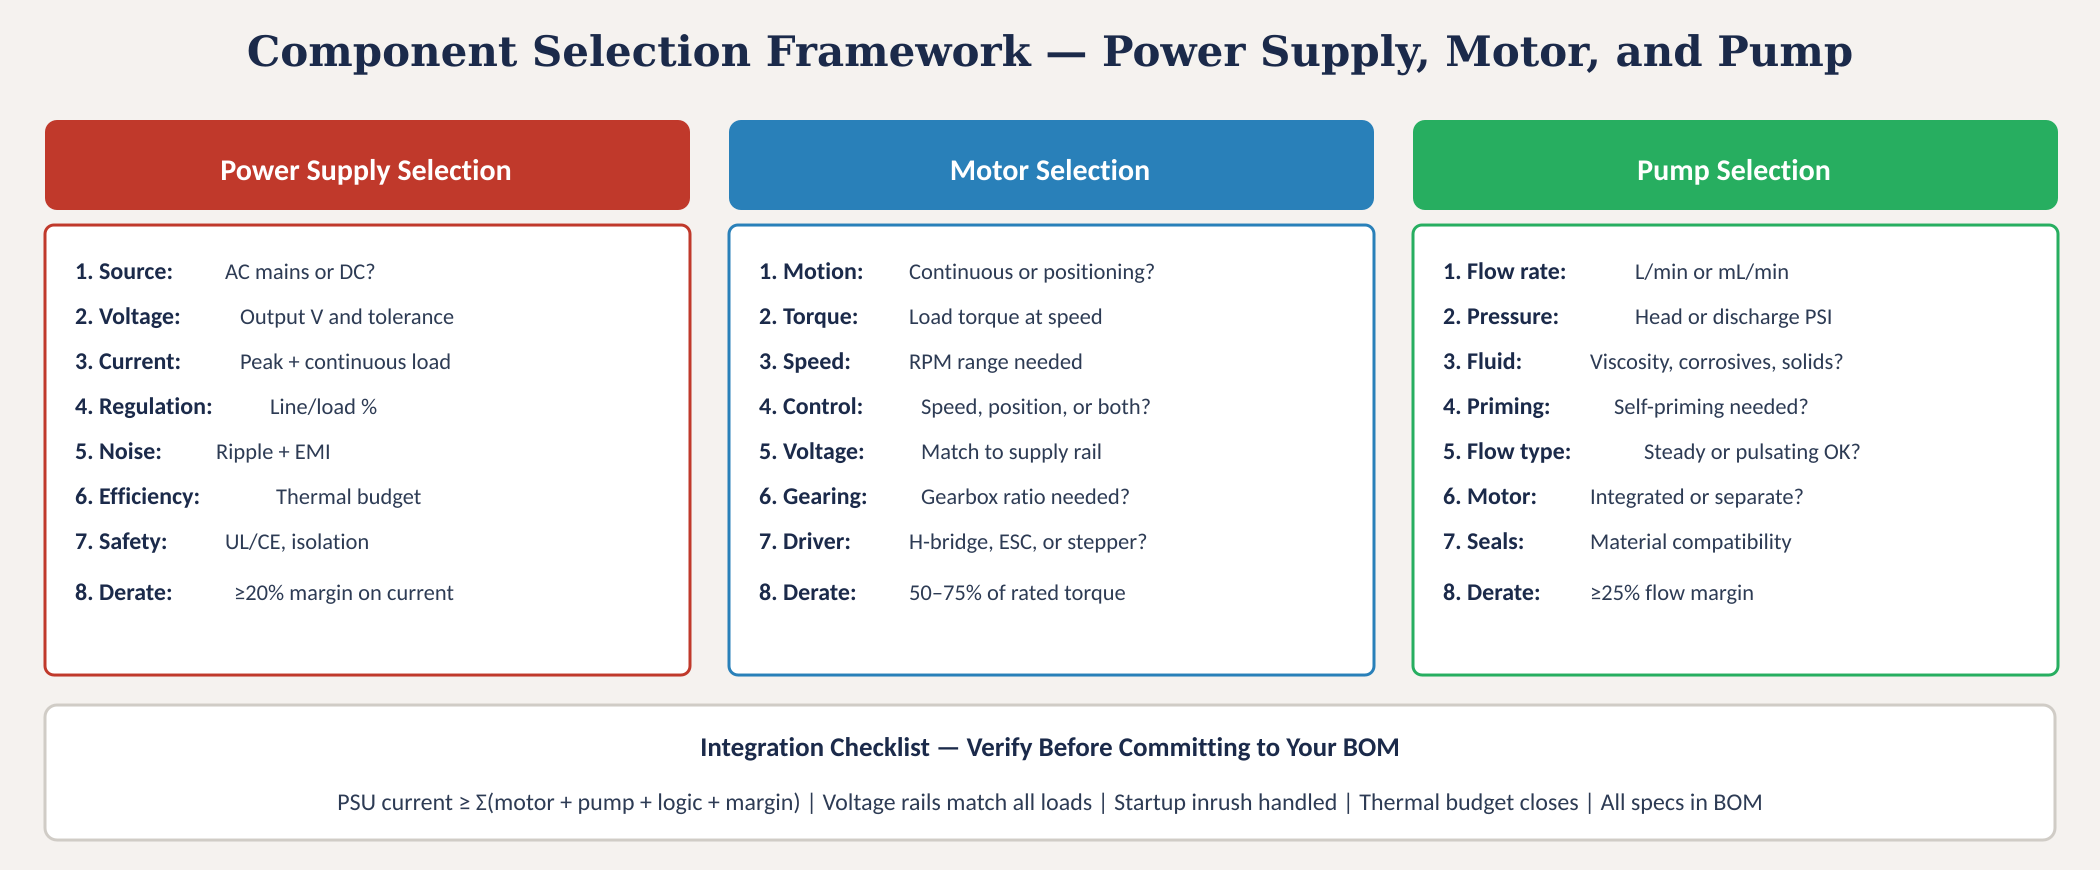
\includegraphics[width=\textwidth]{master_figs/fig_selection_framework.png}
\caption{Parallel selection flows for power supply, motor, and pump with integration verification checklist.}
\label{fig:selection_framework_b}
\end{figure}

\subsection{Design Rules}

\begin{enumerate}[leftmargin=1.5em]
  \item \textbf{Build a power budget spreadsheet first.} List every component with its voltage rail, continuous current, and peak current. Sum the columns. Add 25\% margin.
  \item \textbf{Calculate mechanical load torque before selecting a motor.} $\tau = F \times r$ for linear-to-rotary. Include friction, inertia, and acceleration torque. Select a motor with rated torque $\geq 1.5\times$ your load.
  \item \textbf{For fluid systems, map your complete flow circuit}, pipe lengths, fittings, elevation, filters, to calculate total system head loss. Select a pump whose curve crosses your system curve with margin.
  \item \textbf{Motor inrush is the \#1 power supply problem.} A motor rated at 2\,A running may draw 15\,A at startup. Size your supply for inrush, or use soft-start circuits.
  \item \textbf{Separate power and signal grounds.} Run motor power on dedicated wires back to the supply. Never share ground wires between motors and sensitive electronics.
  \item \textbf{Document everything in your BOM:} part number, manufacturer, voltage, current, torque, flow rate, and procurement source.
\end{enumerate}

\begin{keyconceptbox}[Five Key Takeaways]
\begin{enumerate}[nosep,leftmargin=1.5em]
  \item Power supplies: use pre-certified wall adapters for AC-DC; switching regulators for efficient DC-DC; LDOs only for low-current, noise-sensitive loads.
  \item Motors: match type to control need; brushed DC for simplicity, BLDC for efficiency, stepper for open-loop positioning, servo for closed-loop precision. Every motor needs a driver.
  \item Pumps: positive displacement for precise flow and self-priming; centrifugal for high-volume smooth flow. Match wetted materials to your fluid.
  \item Derating is non-negotiable: 20\% current margin on power supplies, 25--50\% torque margin on motors, 25\% flow margin on pumps.
  \item Integration: build a power budget first, size for inrush, separate power and signal grounds, document every selection in your BOM.
\end{enumerate}
\end{keyconceptbox}


% ══════════════════════════════════════════════════════════════════════
\section{Artifact Handoff: What This Chapter Supports}
\begin{table}[htbp]\centering\small
\begin{tabularx}{\textwidth}{l X l}
\toprule
\textbf{Artifact} & \textbf{Description} & \textbf{Forward Reference} \\
\midrule
Power Budget & Voltage rails, current draws, margin analysis & Ch.~9 (protection), Ch.~5 (integration) \\
Motor Selection & Torque/speed calcs, driver selection, BOM entry & Ch.~11 (transmission), BOM \\
Pump Selection & Flow/pressure calcs, wetted material verification & BOM, test plan \\
\bottomrule
\end{tabularx}
\end{table}

\section{Power Supply Noise and Its Effect on Measurement}
Every switching power supply generates output ripple at the switching frequency (typically 100\,kHz--2\,MHz) and its harmonics. This ripple propagates to every powered circuit, including sensitive analog signal conditioning.

\textbf{Ripple specification}: a ``12\,V, 5\,A'' switching supply may have 50--200\,mV peak-to-peak ripple. For a 14-bit ADC with $\pm$10\,V range (LSB $= 1.22$\,mV), 50\,mV of ripple is 41\,LSBs of noise, potentially dominating the measurement uncertainty.

\textbf{Mitigation}: (1) use a linear post-regulator (LDO) between the switching supply and the analog circuits. The LDO's PSRR (Power Supply Rejection Ratio) attenuates the ripple by 40--70\,dB. A 50\,mV ripple becomes $< 0.05$\,mV after an LDO with 60\,dB PSRR. (2) Add LC filtering: a 100\,$\mu$H inductor followed by 100\,$\mu$F capacitor provides $\sim$40\,dB attenuation at 100\,kHz. (3) Physically separate the analog and digital power paths on the PCB, connecting them only at the power entry point.

\section{Battery Selection for Portable Systems}
\textbf{Lithium Polymer (LiPo)}: 3.7\,V nominal, 4.2\,V charged, 3.0\,V discharged. Energy density: 150--250\,Wh/kg. Most common for student projects. Available in standard sizes from 500\,mAh to 10{,}000\,mAh. Requires BMS (Battery Management System) for charge control and overdischarge protection. \textbf{Never charge unattended; never charge above 4.2\,V; never discharge below 3.0\,V.}

\textbf{Lithium Iron Phosphate (LFP/LiFePO4)}: 3.2\,V nominal. Lower energy density but inherently safer (no thermal runaway). Better cycle life (2000+ vs.\ 500 for LiPo). Preferred for applications where safety is paramount.

\textbf{NiMH}: 1.2\,V nominal. Robust, safe, well-understood. Lower energy density than lithium. Good for applications where cost matters more than weight. Standard AA and AAA sizes simplify replacement.

\textbf{Runtime estimation}: runtime $= C_{\text{battery}}(\text{mAh}) / I_{\text{average}}(\text{mA})$\,hours. A 2000\,mAh battery powering a 200\,mA average load: $2000/200 = 10$\,hours. Derate by 20\% for real-world conditions (self-discharge, temperature, aging): effective runtime $\approx 8$\,hours.
\section{Practice Questions}
% ══════════════════════════════════════════════════════════════════════

\subsection{Conceptual Questions}

\begin{enumerate}[leftmargin=1.5em]
  \item What is the fundamental difference between how a linear regulator and a switching regulator convert voltage?

\begin{keyconceptbox}[Requirements Mapping: From Motor Curves to Shall-Statements]
A motor's torque--speed curve directly generates testable requirements:
\begin{itemize}[nosep,leftmargin=1.5em]
\item ``System shall move payload at 0.5\,m/s'' $\to$ Calculate wheel RPM from diameter, verify the motor's torque at that RPM exceeds load torque with $\geq$50\% margin.
\item ``Motor runs continuously'' $\to$ MOT-REQ: Motor current at operating point shall be $\leq$75\% of continuous rated current. Calculate: $I_{req} = \tau_{load} / K_t$.
\item ``Battery life 4 hours'' $\to$ PSU-REQ: Battery capacity $\geq I_{avg} \times 4 \times 1.3$ (aging margin).
\item ``Pump delivers 2\,L/min at 10\,psi'' $\to$ PUMP-REQ: Pump shall deliver $\geq$2.5\,L/min at $\geq$12\,psi system head loss (25\% margin).
\end{itemize}
If your requirement says ``0.5\,m/s'' but the motor cannot produce the required torque at the corresponding RPM, the requirement and hardware are in conflict. The torque--speed curve resolves this \emph{before} you order parts.
\end{keyconceptbox}

  \item A 12\,V motor has a winding resistance of 0.5\,$\Omega$ and a rated current of 4\,A. What is the stall current? Why is this dangerous?

  \item Explain why a BLDC motor cannot function without an ESC, while a brushed DC motor can operate with just a battery connection.

  \item Your project needs to regulate a LiPo battery (3.0\,--4.2\,V) down to 3.3\,V. Why would a standard buck converter fail during battery discharge?

  \item Compare the self-priming capability of gear pumps versus centrifugal pumps. How does this affect installation design?

  \item Why must you include flyback diodes when driving a motor with an H-bridge? What happens without them?

  \item A power supply is rated at 10\,A at 25\,$^{\circ}$C. If your enclosure reaches 50\,$^{\circ}$C, can you still draw 10\,A? Explain.

  \item What is the primary advantage of a peristaltic pump over a gear pump for biomedical applications?
\end{enumerate}

\subsection{Application / Scenario Questions}

\begin{enumerate}[resume,leftmargin=1.5em]
  \item Your design uses a 24\,V wall adapter powering two DC motors (24\,V, 3\,A each running, 20\,A stall each) and an Arduino (5\,V, 200\,mA). Design the power architecture: what regulators are needed, what is the minimum supply current rating, and how do you handle motor inrush?

  \item You need to pump ethylene glycol coolant at 2\,L/min through a closed cooling loop with 3\,m of tubing, six fittings, and no elevation change. Which pump type do you recommend and why? What seal material?

  \item Your team selects a NEMA 17 stepper for a linear stage. The required force is 20\,N at 50\,mm/s using a 10\,mm lead screw. Calculate the required torque and verify whether a standard NEMA 17 (0.4\,N$\cdot$m rated) is adequate.

  \item \textbf{Diagnostic scenario}: Your prototype's motor operates normally when powered from a bench supply but stutters and resets the microcontroller when powered from the project's 12\,V battery pack. The battery is fully charged. What is the most likely cause, and how do you fix it?
\end{enumerate}

\subsection{Answers}

\begin{enumerate}[leftmargin=1.5em]
  \item A linear regulator dissipates excess voltage as heat (acts as a variable resistor). A switching regulator rapidly switches the input on/off and uses an inductor to transfer energy efficiently, achieving 85--95\% efficiency versus 40--80\% for linear.

  \item $I_{\text{stall}} = V/R = 12/0.5 = 24\,A$; six times the rated current. At stall, all 288\,W ($24 \times 12$) converts to heat in the windings. The motor will overheat and fail within seconds.

  \item A brushed DC motor has mechanical commutation (brushes and commutator) that automatically reverses current in the rotor windings. A BLDC motor's rotor has permanent magnets and the stator windings must be energized in a precise three-phase sequence by the ESC, which reads rotor position via Hall sensors or back-EMF sensing. Without the ESC, there is no commutation and no rotation.

  \item A buck converter requires $V_{\text{in}} > V_{\text{out}}$ to regulate. When the LiPo discharges below 3.3\,V (which happens as the cell depletes toward 3.0\,V), the buck cannot maintain the output. A buck-boost converter is required because it handles the input crossing the output voltage.

  \item Gear pumps are self-priming: they can draw fluid up from below the pump inlet by creating suction through the gear tooth spaces. Centrifugal pumps are not self-priming and require a flooded suction (pump inlet below fluid level). This means centrifugal pumps must be installed below the tank or use a foot valve and check valve to maintain prime.

  \item A motor is an inductive load. When current is suddenly switched off, the collapsing magnetic field generates a voltage spike (back-EMF) that can be many times the supply voltage. Without flyback diodes, this spike destroys the H-bridge transistors. Flyback diodes clamp the spike by providing a current path for the decaying magnetic energy.

  \item No. Every power supply has a thermal derating curve. At 50\,$^{\circ}$C, the supply has less thermal headroom to dissipate heat. A typical derating might reduce capacity to 70--80\% of the 25\,$^{\circ}$C rating, meaning 7\,--8\,A. Always check the datasheet derating curve.

  \item The fluid in a peristaltic pump only contacts the inside of a disposable tube; no seals, rotors, or metal surfaces touch the fluid. This eliminates contamination risk and allows easy sterilization by swapping the tube. A gear pump has fluid contact with gears, housing, and shaft seals, making sterilization far more difficult.

  \item Architecture: wall adapter provides 24\,V rail directly to motors via H-bridges. A buck converter (e.g., LM2596) steps 24\,V down to 5\,V for the Arduino. Minimum supply current: continuous = $2 \times 3 + 0.2 = 6.2\,A$, but inrush = $2 \times 20 = 40\,A$ simultaneously. A 10\,A supply with bulk capacitance ($\geq$4700\,$\mu$F) on the motor rail to absorb inrush, plus staggered motor startup in firmware (start one motor, wait 500\,ms, start the second), is the practical solution.

  \item A small DC centrifugal impeller pump is appropriate: the loop is closed (no priming issue if pump is at the bottom), flow is moderate, ethylene glycol is low viscosity, and smooth non-pulsating flow is preferred for cooling. Seal material: Viton (FKM) or EPDM; both compatible with ethylene glycol at moderate temperatures.

  \item Torque = force $\times$ lead / ($2\pi \times$ efficiency). $\tau = 20 \times 0.010 / (2\pi \times 0.9) = 0.035$\,N$\cdot$m. The NEMA 17 at 0.4\,N$\cdot$m rated torque provides $0.4 / 0.035 = 11.4\times$ margin. However, at the required speed: $50\text{ mm/s} / 10\text{ mm/rev} = 5\text{ rev/s} = 300\text{ RPM}$. Check the stepper's torque-speed curve at 300 RPM; torque typically drops to 40--60\% of holding torque, giving 0.16--0.24\,N$\cdot$m. Still adequate ($4.6$--$6.9\times$ margin), but verify on the actual datasheet curve.

  \item Most likely cause: the battery cannot supply the motor inrush current. Unlike a bench supply (which can deliver virtually unlimited current), a battery has internal resistance. During motor startup, the inrush current ($6$--$10\times$ running) causes a voltage drop across the battery's internal resistance, drooping the 12\,V rail. If it drops below the buck converter's minimum input or the microcontroller's brown-out threshold ($\$\sim\$$2.7\,V for most AVR/ARM), the MCU resets. Fix: add a large bulk capacitor ($\geq$4700\,$\mu$F) on the battery rail close to the motor driver, use a battery with lower internal resistance (higher C-rating), implement soft-start in firmware, and add a separate regulated supply for the MCU with adequate input capacitance.
\end{enumerate}


% ══════════════════════════════════════════════════════════════════════

\chapter{Power Architecture \& Circuit Safety}

\vspace{1em}




\vspace{1em}


% ══════════════════════════════════════════════════════════════════════
\section{Power Architecture}
\label{sec:arch}
% ══════════════════════════════════════════════════════════════════════

\subsection{System-Level Design}

A well-designed power system flows from source through three functional stages before reaching the loads. The \textbf{input stage} is where power enters through a single, well-defined connector. This is where you place first-line protections: a keyed connector (prevents miswiring), reverse polarity protection, an input fuse, and a TVS diode for transient suppression. The \textbf{regulation stage} converts raw input voltage into the specific rails your system needs, commonly cascading from the highest voltage down (e.g., 24\,V input $\to$ 12\,V motor rail $\to$ 5\,V sensor rail $\to$ 3.3\,V MCU rail). The \textbf{distribution stage} delivers regulated power to each load through individual protection, per-rail fuses or electronic current limiters that prevent a fault in one subsystem from cascading.

\begin{figure}[htbp]
\centering
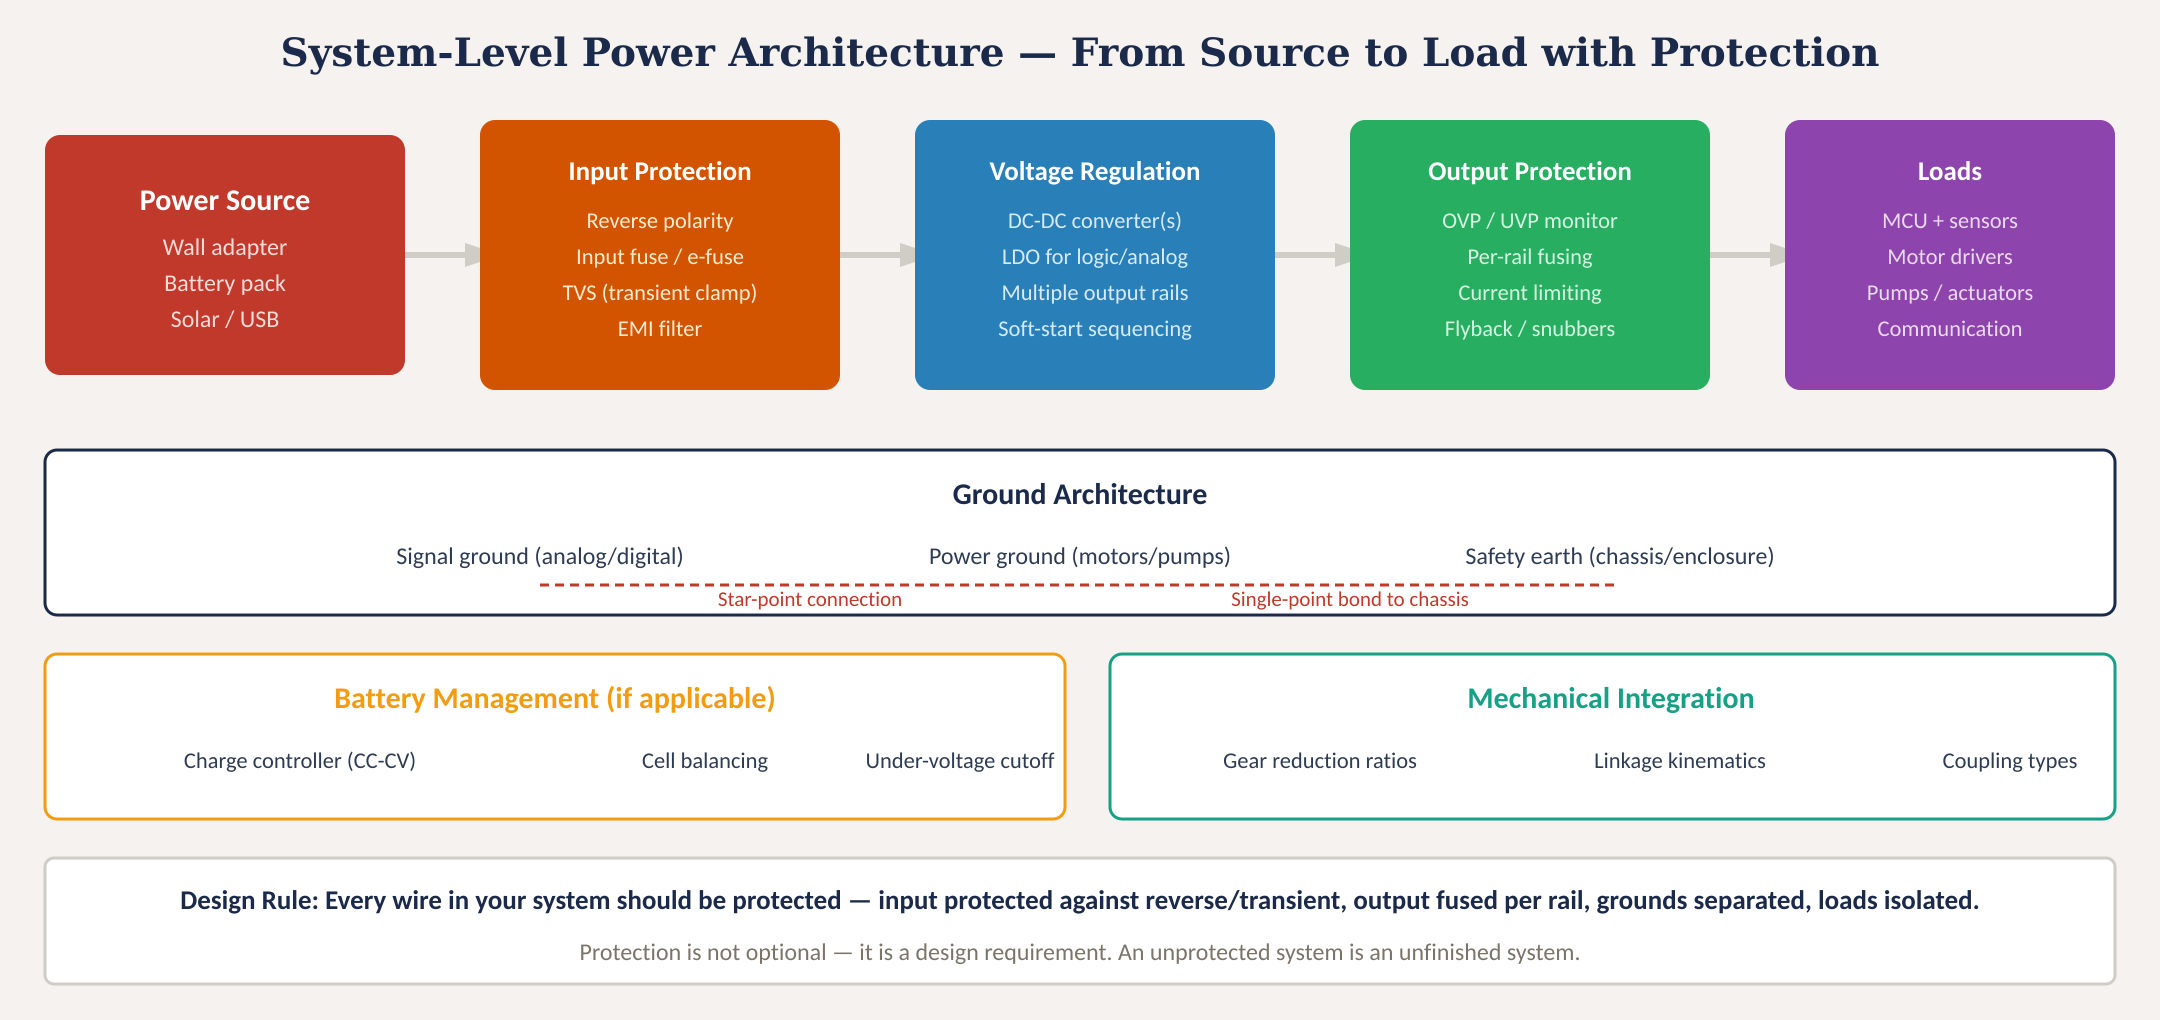
\includegraphics[width=\textwidth]{master_figs/fig_power_architecture.png}
\caption{System-level power architecture from source to load with protection stages, ground architecture, battery management, and mechanical integration.}
\label{fig:architecture}
\end{figure}

\subsection{Grounding Strategy}
\label{sec:grounding}

Ground is not a magical zero-volt reference; it is a real conductor with real resistance and inductance. When a motor draws 5\,A through a ground trace with 50\,m$\Omega$ resistance, there is a 250\,mV drop along that trace. If your ADC's ground reference shares that path, your sensor readings are corrupted.

\subsubsection{Star-Point Grounding}
Run separate ground conductors from each subsystem back to a single point near the power supply. Motor ground, sensor ground, and MCU ground each get their own conductor. They meet at \emph{one star point}. This prevents motor return current from flowing through sensor ground paths.

\subsubsection{Three Ground Domains}
\begin{itemize}[nosep,leftmargin=1.5em]
  \item \textbf{Signal ground}: analog sensors, ADCs, digital logic. Low current, noise-sensitive.
  \item \textbf{Power ground}: motors, pumps, solenoids, heaters. High current, noisy.
  \item \textbf{Safety earth}: metal enclosure, chassis. Fault-current path for AC-powered systems.
\end{itemize}

\begin{warningbox}[The \#1 Debugging Time Sink]
Poor grounding is the single most common cause of difficult-to-diagnose intermittent failures in student projects. If your sensor readings are noisy, your MCU resets when a motor starts, or your serial communication drops characters; check your grounding first.
\end{warningbox}

\subsubsection{AC Mains Safety}
Use a Class~II (double-insulated) wall adapter whenever possible; no earth ground connection is needed. If you must use an internal open-frame supply, bond the metal enclosure to earth ground through a 3-prong inlet with proper strain relief. \textbf{Never defeat a ground prong.}

\subsubsection{Signal Isolation}
Use optocouplers or digital isolators (Si8620, ADUM1201) to pass signals between high-voltage and low-voltage domains. Essential when controlling AC loads (relays, triacs) from a microcontroller.


\subsection{Battery Integration}
\label{sec:battery}

Lithium cells (LiPo, Li-ion, LiFePO\textsubscript{4}) store enormous energy density and can cause fire or explosion if mishandled. A Battery Management System (BMS) is \textbf{mandatory}:

\begin{itemize}[nosep,leftmargin=1.5em]
  \item Overcharge cutoff: 4.2\,V/cell maximum.
  \item Deep-discharge cutoff: 3.0\,V/cell minimum (irreversible damage below this).
  \item Overcurrent / short-circuit shutoff.
  \item Cell balancing for multi-cell packs.
\end{itemize}

Common modules: TP4056 (single-cell charger, CC-CV profile), BQ25895 (buck-boost charger IC), BQ76940 (multi-cell BMS). During development, always store and charge lithium batteries in a fireproof LiPo-safe bag. \textbf{Never charge unattended without a BMS.}

\begin{tipbox}[DC Generation Sources (Solar, Alternator)]
Solar panels produce variable voltage; use an MPPT charge controller to extract maximum power. Always include a blocking diode to prevent battery discharge through the panel at night. For alternators: rectify the AC output, regulate with a charge controller, and add TVS/MOV protection against load-dump voltage spikes if the battery disconnects while the alternator is running.
\end{tipbox}


% ══════════════════════════════════════════════════════════════════════

\subsection{Power Budget Spreadsheet: How to Build One}
The power budget is a spreadsheet with one row per component and the following columns:

\begin{table}[htbp]\centering\small
\begin{tabularx}{\textwidth}{l l c c c X}
\toprule
\textbf{Component} & \textbf{Rail} & \textbf{$I_{typ}$ (mA)} & \textbf{$I_{peak}$ (mA)} & \textbf{Duty (\%)} & \textbf{$I_{avg}$ (mA)} \\
\midrule
ESP32 (active) & 3.3V & 80 & 240 & 10 & 8.0 \\
ESP32 (deep sleep) & 3.3V & 0.01 & --- & 90 & 0.009 \\
DS18B20 sensor & 3.3V & 1.5 & 1.5 & 100 & 1.5 \\
SIM800L (TX) & 4.0V & 200 & 2000 & 1 & 2.0 \\
Relay coil & 12V & 80 & 80 & 5 & 4.0 \\
\midrule
\multicolumn{4}{l}{\textbf{3.3V rail total}} & & \textbf{9.5} \\
\multicolumn{4}{l}{\textbf{3.3V rail peak}} & & \textbf{241.5} \\
\multicolumn{4}{l}{\textbf{12V rail total}} & & \textbf{4.0} \\
\bottomrule
\end{tabularx}
\caption{GreenShield power budget example.}
\end{table}

The peak column sizes your regulators and fuses. The average column sizes your battery. Add 25\% margin to both. If the SIM800L's 2\,A peak on the 4\,V rail shares a regulator with the ESP32, that regulator must handle 2.24\,A peak; a common sizing mistake.

\section{Protection Circuits}
\label{sec:protection}
% ══════════════════════════════════════════════════════════════════════

The philosophy is \textbf{defense in depth}: layer multiple protections so that each catches what the previous one missed. No single device guards against all threats.

\begin{figure}[htbp]
\centering
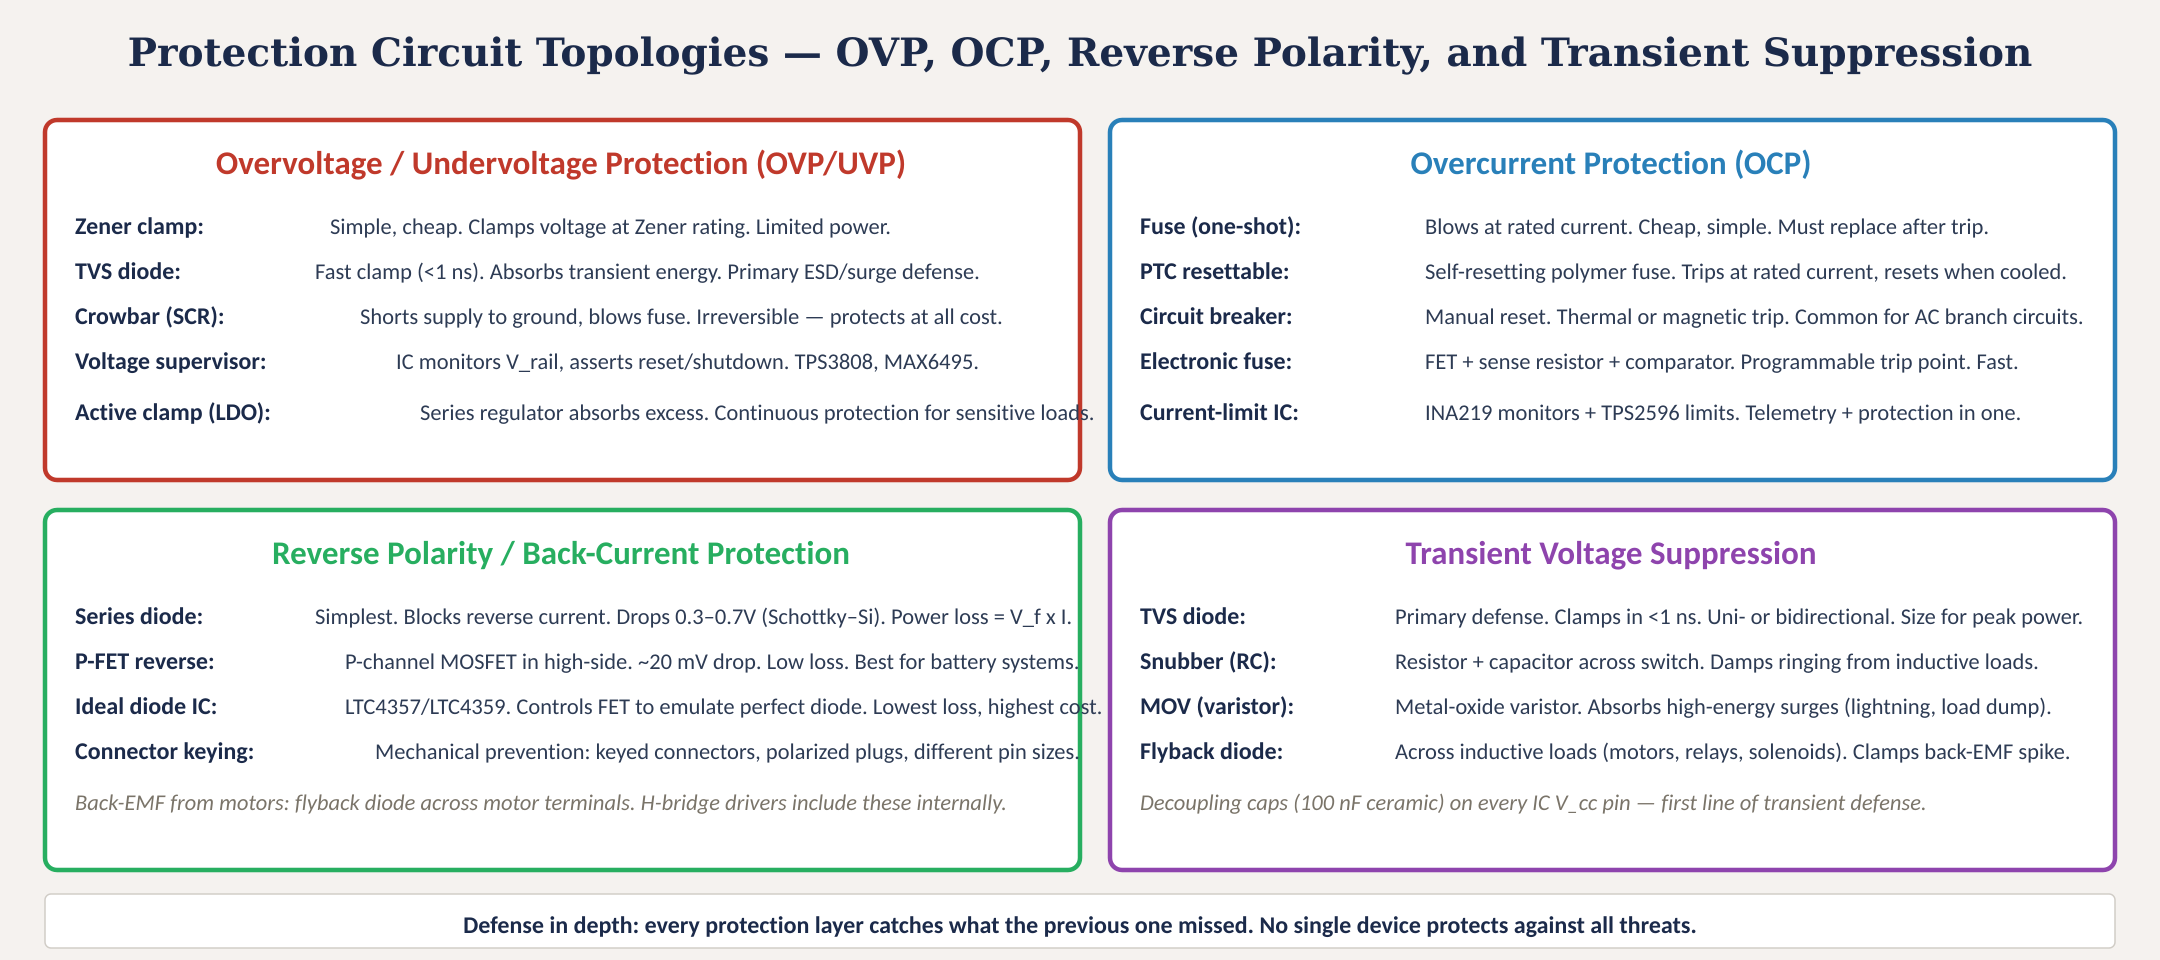
\includegraphics[width=\textwidth]{master_figs/fig_protection_topologies.png}
\caption{Four protection categories: OVP/UVP, OCP, reverse polarity/back-current, and transient suppression with specific device options.}
\label{fig:protection}
\end{figure}


\subsection{Overvoltage and Undervoltage Protection (OVP / UVP)}

\textbf{Overvoltage} pushes components beyond absolute maximum ratings; gate oxide breakdown, latch-up, permanent damage. \textbf{Undervoltage} causes unpredictable behavior: brown-outs, corrupted flash memory, and erratic execution.

\subsubsection{Zener Clamp}
A Zener diode across the supply rail conducts when voltage exceeds its breakdown value, clamping the rail. Simple and cheap but limited by power dissipation ($P = (V_{\text{spike}} - V_Z) \times I$). Select $V_Z$ slightly above your nominal rail (e.g., 5.6\,V Zener for a 5\,V rail).

\subsubsection{TVS Diode}
A Transient Voltage Suppressor; essentially a heavy-duty bidirectional Zener optimized for high peak power. Responds in $<$1\,ns. The primary defense against ESD, inductive spikes, and power supply transients. \textbf{Every power input in a professional design has a TVS diode.}

\textbf{Selection}: standoff voltage $\geq$ operating voltage; clamping voltage $<$ component absolute maximum rating. Common series: SMAJ, SMBJ, 1.5KE.

\subsubsection{Voltage Supervisor IC}
Monitors the supply rail and asserts a reset or shutdown signal when voltage is out of range. Does not clamp; it shuts the system down gracefully. Essential for microcontroller brown-out protection. Common: TPS3808 (adjustable OVP/UVP), MAX6495 (OVP with FET control), TLV803 (simple reset).

\subsubsection{Crowbar Circuit}
An SCR (thyristor) fires when voltage exceeds a threshold, shorting the supply to ground and blowing the upstream fuse. \textbf{Irreversible}; the fuse must be replaced. Used as a last resort when the overvoltage source has enough sustained energy to overwhelm a clamp.


\subsection{Overcurrent Protection (OCP)}
\label{sec:ocp}

Every power rail must have current limiting. A short circuit without protection delivers the full energy of the supply into the fault.

\subsubsection{Fuses (One-Shot)}
A fusible element melts at its rated current. \textbf{Fast-blow} for sensitive electronics; \textbf{slow-blow} (time-delay) for motor circuits where inrush exceeds steady-state. The fuse must blow \emph{before} the wire or component is damaged. Must be accessible for replacement.

\subsubsection{PTC Resettable Fuses}
Polymer PTC (positive temperature coefficient) devices. Resistance increases dramatically at the trip point, limiting current. Self-resets when cooled. Slower than traditional fuses. Best for USB ports and sensor circuits where the fault is intermittent.

\subsubsection{Electronic Fuses (eFuse)}
A MOSFET in series with the load, controlled by a current-sense amplifier. Programmable trip point, fast response, automatic retry or latched shutdown. Provides current \emph{limiting} (not just cutting); can hold current at a safe level during motor inrush. Common: TPS2596, LTC4368, MAX14690.

\subsubsection{Circuit Breakers}
Thermal or magnetic trip mechanism with manual reset. Common for AC branch circuits (15\,A, 20\,A per NEC). In DC systems, used for battery main disconnects. \textbf{Must be DC-rated}; an AC breaker may not safely interrupt DC arcs because DC does not cross zero.

\begin{warningbox}[Fuse + Wire Sizing Rule]
The fuse must blow before the wire overheats. This means the fuse rating must be \emph{below} the wire's ampacity. Size them together using NEC Table 310.16 or AWG ampacity charts: the fuse protects the wire, the wire carries the current, and the load defines the requirement.
\end{warningbox}


\subsection{Reverse Polarity and Back-Current Protection}
\label{sec:reverse}

A battery connected backwards forward-biases body diodes of every downstream MOSFET and IC, often destroying the entire board in milliseconds.

\subsubsection{Series Diode}
Simplest approach. A Schottky diode ($\$\sim\$$0.3\,V drop) or silicon diode ($\$\sim\$$0.7\,V drop) in the positive rail blocks reverse current. Power loss = $V_f \times I_{\text{load}}$. Best for low-current ($<$2\,A) circuits where the voltage drop is acceptable.

\subsubsection{P-Channel MOSFET}
A P-FET in the high-side power path conducts when polarity is correct (body diode initially conducts, pulling gate low, fully enhancing the FET) and blocks when reversed. Voltage drop = $I \times R_{DS(\text{on})}$, typically 10\,--50\,m$\Omega$. At 5\,A with 20\,m$\Omega$: only 0.1\,V drop, 0.5\,W loss. \textbf{Best for battery-powered systems.} Common: Si2301, IRLML6402, DMG2307L.

\subsubsection{Ideal Diode IC}
An IC controlling an external N-FET to emulate a perfect diode with $\$\sim\$$20\,mV forward drop. Lowest loss, fastest reverse blocking, highest cost. LTC4357, LTC4359, MAX40200. Also used for OR-ing redundant supplies and solar/battery combining.

\subsubsection{Mechanical Prevention}
Keyed connectors, polarized plugs, and different-sized pins physically prevent reverse connection. The first line of defense. Always use polarized connectors for DC power.


\subsection{Transient Voltage Suppression}
\label{sec:transient}

Every time you switch an inductive load, motor, relay, solenoid, you create a voltage transient. The physics: $V = -L \times dI/dt$. Current cannot change instantaneously in an inductor, so the collapsing magnetic field generates a spike that can reach hundreds of volts from a 12\,V motor.

\begin{figure}[htbp]
\centering
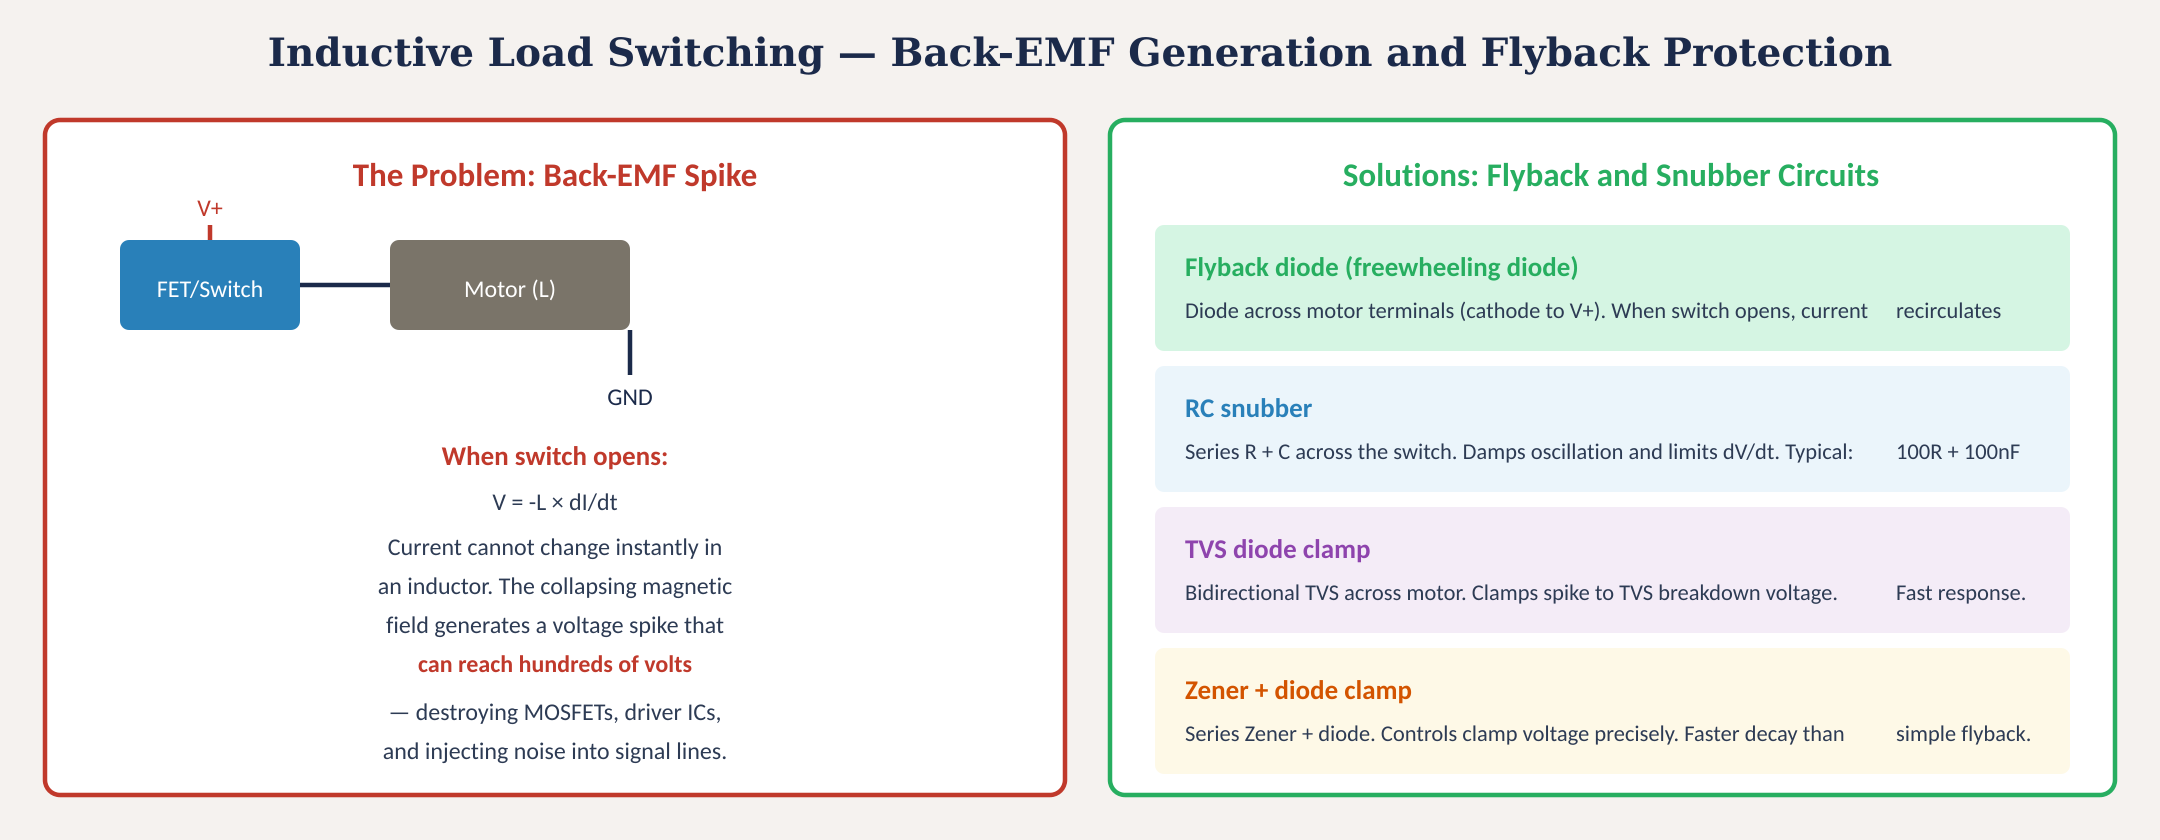
\includegraphics[width=\textwidth]{master_figs/fig_back_emf.png}
\caption{Back-EMF generation from inductive load switching and four protection solutions: flyback diode, RC snubber, TVS clamp, and Zener+diode.}
\label{fig:backemf}
\end{figure}

\subsubsection{Flyback Diode (Freewheeling Diode)}
\textbf{The single most important protection for inductive loads.} A diode across the motor, relay, or solenoid (cathode to V+) provides a current path when the switch opens. Without it, the collapsing field generates a spike that destroys the switching device. Use a fast-recovery or Schottky diode. H-bridge driver ICs include these internally, but if you drive a relay or solenoid with a bare MOSFET, you \textbf{must} add one externally.

\subsubsection{RC Snubber}
A resistor-capacitor network across a switch or relay contact. The capacitor absorbs the initial spike; the resistor dissipates energy and damps oscillation. Typical starting values: 100\,$\Omega$ + 100\,nF for relay contacts. Tune by observing the transient on an oscilloscope.

\subsubsection{TVS Diode (Board-Level)}
Place a TVS across each power rail at the board edge where external cables connect. Absorbs energy from ESD, cable transients, and motor switching spikes propagating through the power bus.

\subsubsection{Decoupling Capacitors}
100\,nF ceramic capacitors on \textbf{every} IC $V_{CC}$ pin, as close to the pin as physically possible. These absorb high-frequency transients before they reach the IC. For power regulators, add bulk capacitance (10\,--100\,$\mu$F) per the datasheet. \textbf{Decoupling is not optional.}


% ══════════════════════════════════════════════════════════════════════
\section{Electromechanical Integration}
\label{sec:mechint}
% ══════════════════════════════════════════════════════════════════════

\begin{figure}[htbp]
\centering
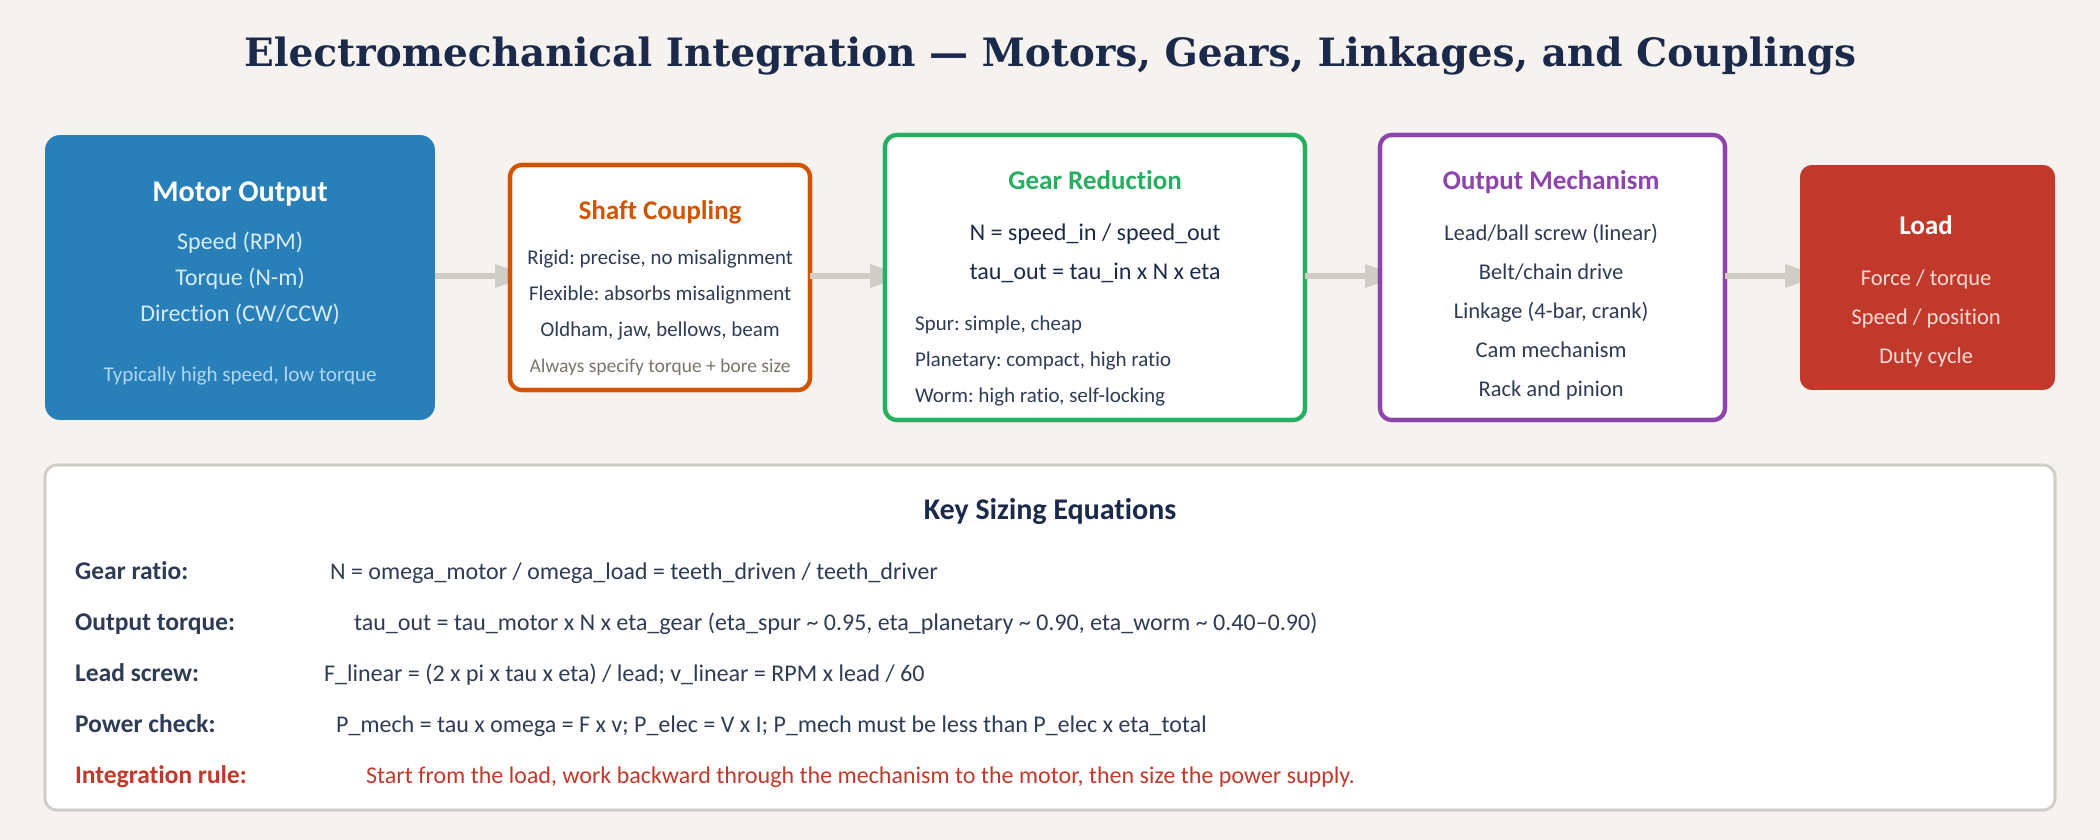
\includegraphics[width=\textwidth]{master_figs/fig_mech_integration.png}
\caption{Motor-to-load power flow through coupling, gear reduction, and output mechanism with key sizing equations.}
\label{fig:mech}
\end{figure}

\subsection{Gear Reduction}

Motors run efficiently at high speed and low torque. Loads typically need the opposite. Gearboxes trade speed for torque:
\begin{equation}
  \tau_{\text{out}} = \tau_{\text{motor}} \times N \times \eta_{\text{gear}}
\end{equation}
where $N$ is the gear ratio ($\omega_{\text{in}} / \omega_{\text{out}}$) and $\eta$ is the gearbox efficiency.

\begin{table}[htbp]
\centering\small
\begin{tabularx}{\textwidth}{l l X}
  \toprule
  \textbf{Type} & \textbf{Efficiency} & \textbf{Characteristics} \\
  \midrule
  Spur & 95--98\% & Simplest, cheapest. External parallel-axis mesh. Available in stock gearmotors. \\
  Planetary & 85--95\%/stage & Compact, coaxial, high torque density. 3:1 to 100:1 per stage. \\
  Worm & 40--90\% & Very high ratios (20:1--300:1) in one stage. Self-locking at high ratios. \\
  \bottomrule
\end{tabularx}
\caption{Gear reduction types and efficiencies.}
\end{table}

\subsection{Output Mechanisms}

\begin{itemize}[leftmargin=1.5em]
  \item \textbf{Shaft couplings}: rigid (zero misalignment tolerance) or flexible (jaw, Oldham, bellows, beam). Beam couplings are the standard for stepper motors.
  \item \textbf{Lead/ball screws}: convert rotary to linear. $F = 2\pi \tau \eta / \text{lead}$. Lead screws are self-locking; ball screws are not.
  \item \textbf{Timing belt drives} (GT2, HTD): positive engagement, no slip. Standard for CNC and 3D printers.
  \item \textbf{Linkages} (4-bar, crank-slider, cam): complex output paths. Torque varies through the cycle; size the motor for peak, not average.
\end{itemize}

\begin{keyconceptbox}[Integration Rule]
\textbf{Start from the load and work backward}: calculate the force/torque and speed the load requires $\to$ select the mechanism and gear ratio $\to$ calculate the motor torque $\to$ select the motor $\to$ calculate the current draw $\to$ size the power supply. The power check: $P_{\text{mech}} = \tau \omega = F v$ must be $\leq P_{\text{elec}} \times \eta_{\text{total}}$.
\end{keyconceptbox}


% ══════════════════════════════════════════════════════════════════════
\section{Safety Design Checklist}
\label{sec:checklist}
% ══════════════════════════════════════════════════════════════════════

Every item must be addressed before commissioning:

\begin{enumerate}[leftmargin=1.5em]
  \item Input has reverse polarity protection (P-FET or series diode).
  \item Input has a fuse or electronic current limiter rated for expected peak current.
  \item TVS diode on every power input where external cables connect.
  \item Voltage supervisor on MCU power rail (brown-out reset).
  \item Flyback diode on every inductive load not protected by the driver IC.
  \item Per-rail fusing; each output rail has its own current protection.
  \item 100\,nF decoupling capacitor on every IC $V_{CC}$ pin.
  \item Signal and power grounds separated, joined at a single star point.
  \item Enclosure bonded to earth ground (if using internal AC-DC supply).
  \item All wire gauges sized for their maximum current with appropriate derating.
\end{enumerate}

\begin{keyconceptbox}[Requirements Mapping: From Protection Specs to Shall-Statements]
Protection circuit design generates system requirements:
\begin{itemize}[nosep,leftmargin=1.5em]
\item ``System survives reverse battery'' $\to$ SYS-REQ: The power input shall include reverse-polarity protection limiting leakage to $<$1\,mA.
\item ``Motor inrush must not reset MCU'' $\to$ PWR-REQ: The MCU supply rail shall maintain $\geq$2.7\,V during motor inrush transients up to 15\,A for 100\,ms.
\item ``ESD at user connectors'' $\to$ SYS-REQ: User-accessible interfaces shall withstand $\pm$8\,kV contact discharge per IEC 61000-4-2.
\end{itemize}
Build your power budget spreadsheet \emph{first}, then derive protection requirements from worst-case currents and voltages.
\end{keyconceptbox}


% ══════════════════════════════════════════════════════════════════════
\section{Grounding Architecture}
The grounding strategy is the single most impactful decision for system noise performance:

\textbf{Single-point (star) ground}: all ground returns converge at one physical point. Prevents ground loops (current from one subsystem flowing through another's ground return and creating noise). The star point is typically at the power entry connector. This is the standard for mixed analog/digital systems.

\textbf{Multi-point ground}: each subsystem connects to the nearest ground plane point. Used in high-frequency systems ($>$1\,MHz) where the inductance of long ground wires to the star point would cause resonance. For MEGN~301 projects operating below 1\,MHz: use star grounding.

\textbf{Split ground plane}: on the PCB, use a continuous ground plane under the analog section and a separate continuous ground plane under the digital section, connected at a single point (the star bridge). This prevents digital switching current from flowing under the analog circuits, which would inject noise.

\section{Electromagnetic Compatibility (EMC) Basics}
Every MEGN~301 system is both an EMI source (motors, switching regulators, digital clocks radiate) and an EMI victim (sensors, ADCs, communication lines are susceptible). Basic EMC design rules:

\textbf{Minimize loop areas}: the magnetic field radiated by a current loop is proportional to the loop area. Keep the current path and its return path as close together as possible. A ground plane provides the minimum-area return path for every trace above it.

\textbf{Filter at boundaries}: when a signal enters or leaves the system enclosure, it should pass through a filter (RC low-pass for analog signals, ferrite bead for digital signals, TVS diode for ESD protection). The enclosure boundary is where external EMI enters and internal EMI escapes.

\textbf{Separate noisy and sensitive circuits}: physically separate motor drivers, switching regulators, and high-speed digital circuits from analog sensors and amplifiers. On a PCB: place them on opposite sides. In an enclosure: use separate compartments or shielding barriers.

\textbf{Decouple every IC}: 100\,nF ceramic capacitor within 5\,mm of every IC power pin. This provides local charge storage for fast switching transients, preventing them from propagating through the power bus to other ICs.
\section{Practice Questions}
\label{sec:practice}
% ══════════════════════════════════════════════════════════════════════

\subsection{Conceptual Questions}

\begin{enumerate}[leftmargin=1.5em]
  \item Explain why star-point grounding prevents motor noise from corrupting ADC readings. What happens if motor current returns through a shared ground trace?

  \item A TVS diode has a standoff voltage of 12\,V and a clamping voltage of 19.9\,V at 10\,A. Is this suitable for protecting a 12\,V circuit whose components have a 20\,V absolute maximum rating?

  \item Compare a series Schottky diode versus a P-channel MOSFET for reverse polarity protection at 5\,A. Calculate the power loss for each (Schottky $V_f = 0.3\,V$, P-FET $R_{DS(\text{on})} = 20\,\text{m}\Omega$).

  \item Why must a DC circuit breaker be specifically rated for DC voltage? What is the hazard of using an AC-rated breaker on a DC circuit?

  \item A relay coil has 50\,mH inductance and draws 100\,mA at 12\,V. If the switch opens in 1\,$\mu$s, estimate the back-EMF spike voltage ($V = L \times dI/dt$). Why does this destroy a 60\,V MOSFET?

  \item What is the difference between a crowbar circuit and a TVS diode clamp? When would you use each?

  \item Explain why decoupling capacitors must be placed as close to the IC power pin as possible, not just ``somewhere on the same board.''
\end{enumerate}

\subsection{Application / Scenario Questions}

\begin{enumerate}[resume,leftmargin=1.5em]
  \item Your robot uses a 4S LiPo battery (14.8\,V nominal, 16.8\,V max charge, 12.0\,V cutoff) powering two DC motors (5\,A each continuous, 30\,A each stall), a Raspberry Pi (5\,V, 2.5\,A), and three servos (6\,V, 1\,A each peak). Design the complete power architecture: draw a block diagram showing every rail, regulator, and protection device. Specify part numbers where possible.

  \item Your project team's prototype works perfectly on the bench but fails intermittently in the field. Symptoms: the motor runs fine, but the microcontroller occasionally resets, and analog sensor readings drift by 200\,mV when the motor switches direction. Diagnose the root cause and propose a fix using concepts from this module.

  \item A classmate argues that a flyback diode is unnecessary because ``the motor driver IC already handles back-EMF.'' Under what conditions is the classmate correct? Under what conditions is the classmate dangerously wrong?

  \item Design a protection scheme for a solar panel (18\,V open-circuit, 5\,A short-circuit) charging a 3S LiPo (11.1\,V nominal) that also powers a 12\,V water pump. Include reverse-current blocking, charge control, and load protection.
\end{enumerate}

\subsection{Answers}

\begin{enumerate}[leftmargin=1.5em]
  \item In a shared ground, motor current ($I_M$) flows through the same trace as sensor return current. The trace has resistance $R$, so the sensor sees a ground voltage offset of $V_{\text{noise}} = I_M \times R$. With star-point grounding, motor current returns through its own dedicated conductor, so the sensor ground conductor carries only the small sensor current. The noise voltage on the sensor ground drops from $I_M \times R$ to $I_{\text{sensor}} \times R$, which is typically orders of magnitude smaller.

  \item Yes; the standoff voltage (12\,V) is at or above the operating voltage, so the TVS does not conduct during normal operation. The clamping voltage (19.9\,V) is below the 20\,V absolute maximum, so the TVS clamps before the components are damaged. However, the margin is very tight (0.1\,V). A TVS with a 16.7\,V or lower clamping voltage would provide better margin. Always verify the clamping voltage at the expected peak current, not just the rated value.

  \item Schottky: $P = V_f \times I = 0.3 \times 5 = 1.5\,W$. P-FET: $P = I^2 \times R_{DS} = 25 \times 0.020 = 0.5\,W$. The P-FET dissipates one-third the power. At 5\,A, the Schottky also drops the voltage rail by 0.3\,V, which may push the rail below the minimum operating voltage of downstream components. The P-FET drops only 0.1\,V. For battery-powered systems where efficiency and voltage headroom matter, the P-FET is strongly preferred.

  \item AC current crosses zero 120 times per second (at 60\,Hz), which naturally extinguishes any arc at the breaker contacts. DC current never crosses zero, so a DC arc can sustain indefinitely. An AC-rated breaker's contacts and arc chute may not be designed to extinguish a sustained DC arc, potentially causing the breaker to fail to interrupt the circuit, or worse, catch fire internally.

  \item $V = L \times dI/dt = 0.050 \times (0.100 / 0.000001) = 5000\,V$. This 5\,kV spike (in theory) far exceeds the 60\,V MOSFET's drain-source breakdown voltage. In practice, the MOSFET avalanches and the spike is clamped at the breakdown voltage, but the energy dissipated during avalanche can destroy the device. A flyback diode clamps the spike to approximately $V_{\text{supply}} + V_f \approx 12.7\,V$, well within the MOSFET's rating.

  \item A TVS diode \emph{clamps} the voltage; it conducts just enough to limit the voltage and absorbs the transient energy, then stops conducting when the voltage returns to normal. Operation is non-destructive. A crowbar circuit \emph{shorts} the supply to ground via an SCR, deliberately blowing the upstream fuse. It is destructive (fuse replacement required) but provides guaranteed protection when the overvoltage has enough sustained energy to overwhelm a TVS. Use TVS for transient spikes (ESD, inductive switching); use crowbar for sustained overvoltage from a failed regulator.

  \item Decoupling caps work by providing a low-impedance path for high-frequency transients to bypass the IC rather than entering through the power pins. The trace between the capacitor and the IC pin has inductance proportional to its length. A long trace adds enough inductance to negate the capacitor's effectiveness at high frequencies. Placing the cap within a few millimeters of the pin minimizes this parasitic inductance and keeps the bypass impedance low at the frequencies where transients occur.

  \item Architecture: Battery $\to$ main fuse (80\,A, covers dual motor stall) $\to$ reverse polarity P-FET (IRLML6402 or similar) $\to$ TVS diode (18\,V standoff) $\to$ power distribution bus. Motor rail: direct from battery through individual 40\,A slow-blow fuses per motor, H-bridge drivers with integrated flyback diodes. 5\,V rail: buck converter (e.g., LM2596 or MP1584, 3A rated) from battery bus, with 100\,$\mu$F bulk cap + 100\,nF ceramic decoupling. 6\,V servo rail: buck converter (adjustable output set to 6\,V, 5A rated, TPS54560) with per-servo PTC fuses. BMS: 4S BMS module with 12.0\,V cutoff, 16.8\,V overcharge protection, and cell balancing. Grounds: star-point near main fuse; separate motor ground bus and logic ground bus.

  \item Root cause: ground-coupled motor noise. When the motor reverses direction via the H-bridge, the current transient creates a voltage spike on the shared ground that (a) momentarily shifts the MCU's ground reference, triggering a brown-out reset, and (b) offsets the ADC's reference voltage by 200\,mV, corrupting readings. Fix: (a)~separate motor power ground and MCU signal ground, joining at a star point near the battery; (b)~add a voltage supervisor (TPS3808) on the MCU rail to hold the MCU in clean reset during transients rather than allowing corrupted execution; (c)~add bulk capacitance (470\,$\mu$F) on the MCU's supply rail to absorb the transient; (d)~add a TVS diode on the motor power bus.

  \item The classmate is correct when using a properly rated H-bridge driver IC (like L298N, DRV8871, BTS7960) that includes integrated flyback/freewheeling diodes across the output MOSFETs. These diodes handle the back-EMF from the motor. The classmate is \textbf{dangerously wrong} when: (a)~driving a relay, solenoid, or valve directly from a bare MOSFET or BJT; these loads have no integrated protection; (b)~the motor's back-EMF exceeds the driver's clamping capability; or (c)~using a driver module where the ``protection diodes'' are actually for the logic section, not the motor outputs. \textbf{Rule}: verify in the driver's datasheet that flyback diodes are explicitly rated for the motor's inductive energy.

  \item Solar input: blocking diode (Schottky, e.g., MBR2045) prevents battery discharge through panel at night. MPPT charge controller (e.g., Genasun GV-5 or Victron 75/15) sized for 3S LiPo with 12.6\,V charge termination. Reverse polarity: P-FET on both the solar input and the battery connector. TVS diode (18\,V standoff) on the solar input for transient protection. Load: battery feeds pump through a slow-blow fuse (3\,A for a 2\,A pump). Flyback diode across pump motor terminals. Voltage supervisor monitors battery voltage and disables pump via a load switch when battery drops below 10.5\,V to protect cells. The charge controller's MPPT algorithm ensures maximum solar harvest even as panel voltage varies with sun angle and temperature.
\end{enumerate}


% ══════════════════════════════════════════════════════════════════════



\chapter{Mechanical Fasteners \& Bearings}

\vspace{1em}

Every mechanical system is held together by fasteners and supported by bearings. Selecting the wrong bolt grade, under-torquing a critical joint, or choosing a bearing that cannot handle the load will cause your system to fail; often catastrophically and without warning. This chapter covers the fastener and bearing knowledge you need to specify these components correctly in your BOM and engineering drawings.

\vspace{1em}

\section{Threaded Fasteners}

\subsection{Bolt and Screw Anatomy}
A threaded fastener converts rotational torque into axial clamping force (preload) that holds a joint together. Key parameters: \textbf{nominal diameter} (major diameter, e.g., M6 = 6\,mm), \textbf{pitch} (distance between threads; metric specifies pitch in mm; imperial uses TPI), \textbf{thread length}, and \textbf{head type} (hex, socket, flat, pan, button).

\textbf{Bolts} pass through clearance holes and clamp with a nut. \textbf{Screws} thread into a tapped hole. \textbf{Machine screws} use fine threads in tapped metal. \textbf{Self-tapping screws} form their own threads in plastic or sheet metal.

\subsection{Thread Standards}

\begin{tipbox}[Metric and Imperial Do Not Mix]
M6$\times$1.0 and 1/4-20 UNC look nearly identical (6.0\,mm vs.\ 6.35\,mm diameter). They will partially engage but strip immediately under load. Always verify with a thread gauge or package markings.
\end{tipbox}

\textbf{Unified (inch)}: UNC (Coarse) for general assembly, fewer turns, tolerant of damage. UNF (Fine) for vibration-sensitive and precision applications. \textbf{Metric (ISO)}: Designated M$d \times p$ (e.g., M6$\times$1.0). Coarse pitch is the default. Fine pitch for vibration resistance. Metric is the global standard, use for new designs unless interfacing with existing inch hardware.

\subsection{Bolt Grades and Strength}

\begin{figure}[htbp]\centering
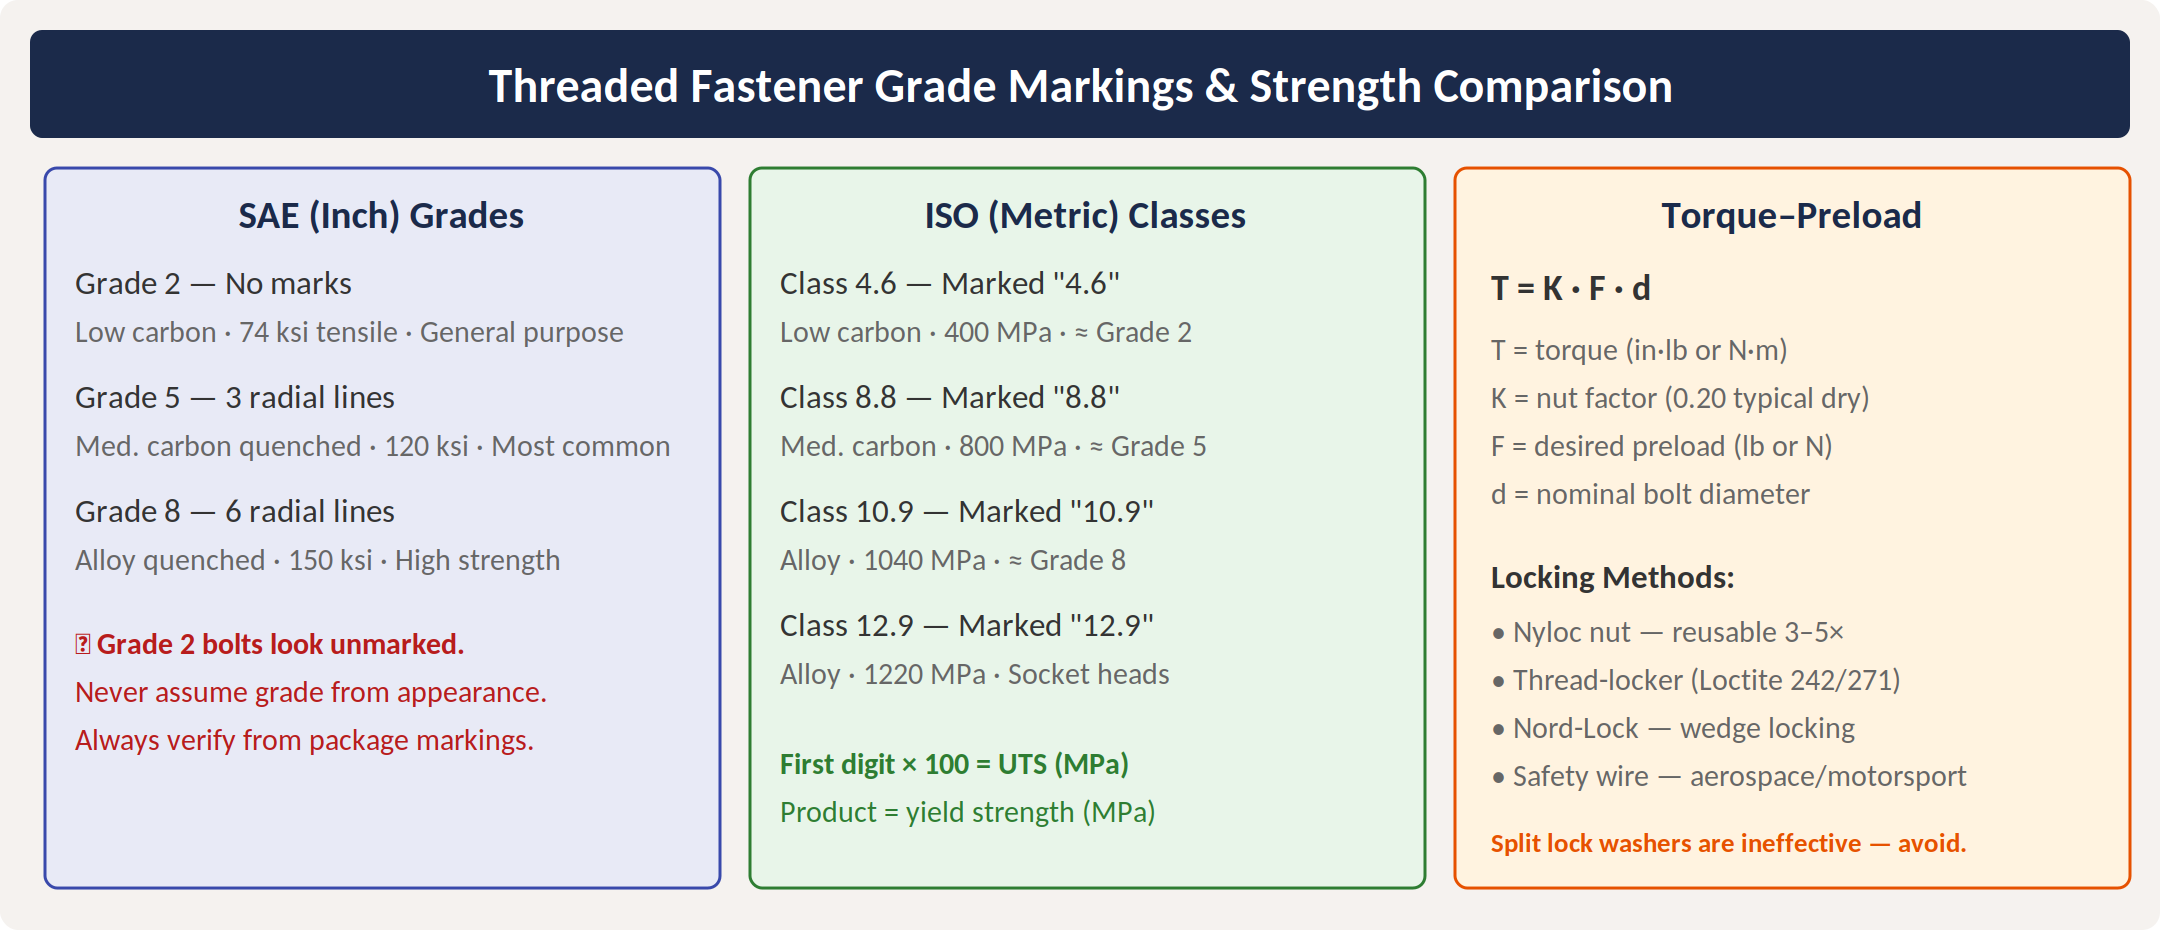
\includegraphics[width=\textwidth]{master_figs/fig_bolt_grades.png}
\caption{SAE and ISO bolt grade markings with strength data and torque-preload relationship.}\label{fig:grades}
\end{figure}

\textbf{SAE (inch)}: Grade~2 (no marks, 74\,ksi, general purpose), Grade~5 (3 radial lines, 120\,ksi, most common structural), Grade~8 (6 radial lines, 150\,ksi, high strength). \textbf{ISO (metric)}: Class~4.6 ($\approx$ Gr.~2), 8.8 ($\approx$ Gr.~5), 10.9 ($\approx$ Gr.~8), 12.9 (socket heads, 1220\,MPa). The first digit $\times$100 gives the UTS in MPa; the product of digits gives yield.

\begin{tipbox}[Specify the Grade]
Never list just ``M6 hex bolt'' in your BOM. Always specify: M6$\times$1.0$\times$25, Class 8.8, zinc plated. Missing the grade means the vendor ships 4.6 at half the strength.
\end{tipbox}

\subsection{Torque and Preload}
The purpose of tightening a bolt is to generate \textbf{preload} (clamping force). The torque-preload relationship:
\begin{equation}
T = K \cdot F \cdot d
\end{equation}
where $T$ = applied torque, $K$ = nut factor (0.20 dry steel, 0.15 lubricated, 0.12 anti-seize), $F$ = desired preload (typically 75\% of proof load), $d$ = nominal diameter. \textbf{90\% of applied torque is lost to friction}; only 10\% generates clamping force.

\subsection{Locking Methods}
Vibration loosens fasteners. Four reliable methods:
\begin{itemize}[nosep,leftmargin=1.5em]
\item \textbf{Nyloc nut}: nylon insert deforms around threads. Reusable 3--5$\times$. Max 120\,\degC{}.
\item \textbf{Thread-locker}: Loctite 242 (blue, removable) for general use; 271 (red, permanent) for critical joints.
\item \textbf{Nord-Lock washers}: wedge-locking. Positive mechanical lock independent of friction. Gold standard.
\item \textbf{Safety wire}: drilled bolt heads wired in pairs. Aerospace and motorsport.
\end{itemize}

\begin{tipbox}[Split Lock Washers Are Ineffective]
Despite ubiquity, split lock washers have been shown in NASA and Junker vibration testing to provide no meaningful locking action. They flatten at low preloads. Use nyloc nuts or thread-locker instead.
\end{tipbox}

\subsection{Non-Threaded Fasteners}
\textbf{Rivets}: permanent fasteners for sheet materials. Blind (pop) rivets install from one side. \textbf{Pins}: dowel (precision alignment), roll/spring (self-retaining), clevis (quick connect/disconnect for linkages). \textbf{Retaining rings}: external E-clips on shafts, internal in bores; inexpensive axial retention for bearings and gears. \textbf{Snap-fits}: integral plastic features; cantilever design with strain $\leq$2\% for ABS, $\leq$4\% for PP.

\begin{tipbox}[MEGN 301 Sourcing]
McMaster-Carr ships next-day to Golden and stocks every fastener here. Bolt Depot and Albany County Fasteners for bulk. For 3D-printed snap-fits, prototype in PLA, final in PETG or nylon.
\end{tipbox}

\section{Bearings}
\subsection{What Bearings Do}
Bearings support a rotating or sliding shaft while minimizing friction. Every bearing balances: \textbf{load capacity}, \textbf{speed}, \textbf{precision}, and \textbf{life}.

\subsection{Bearing Types}
\begin{figure}[htbp]\centering
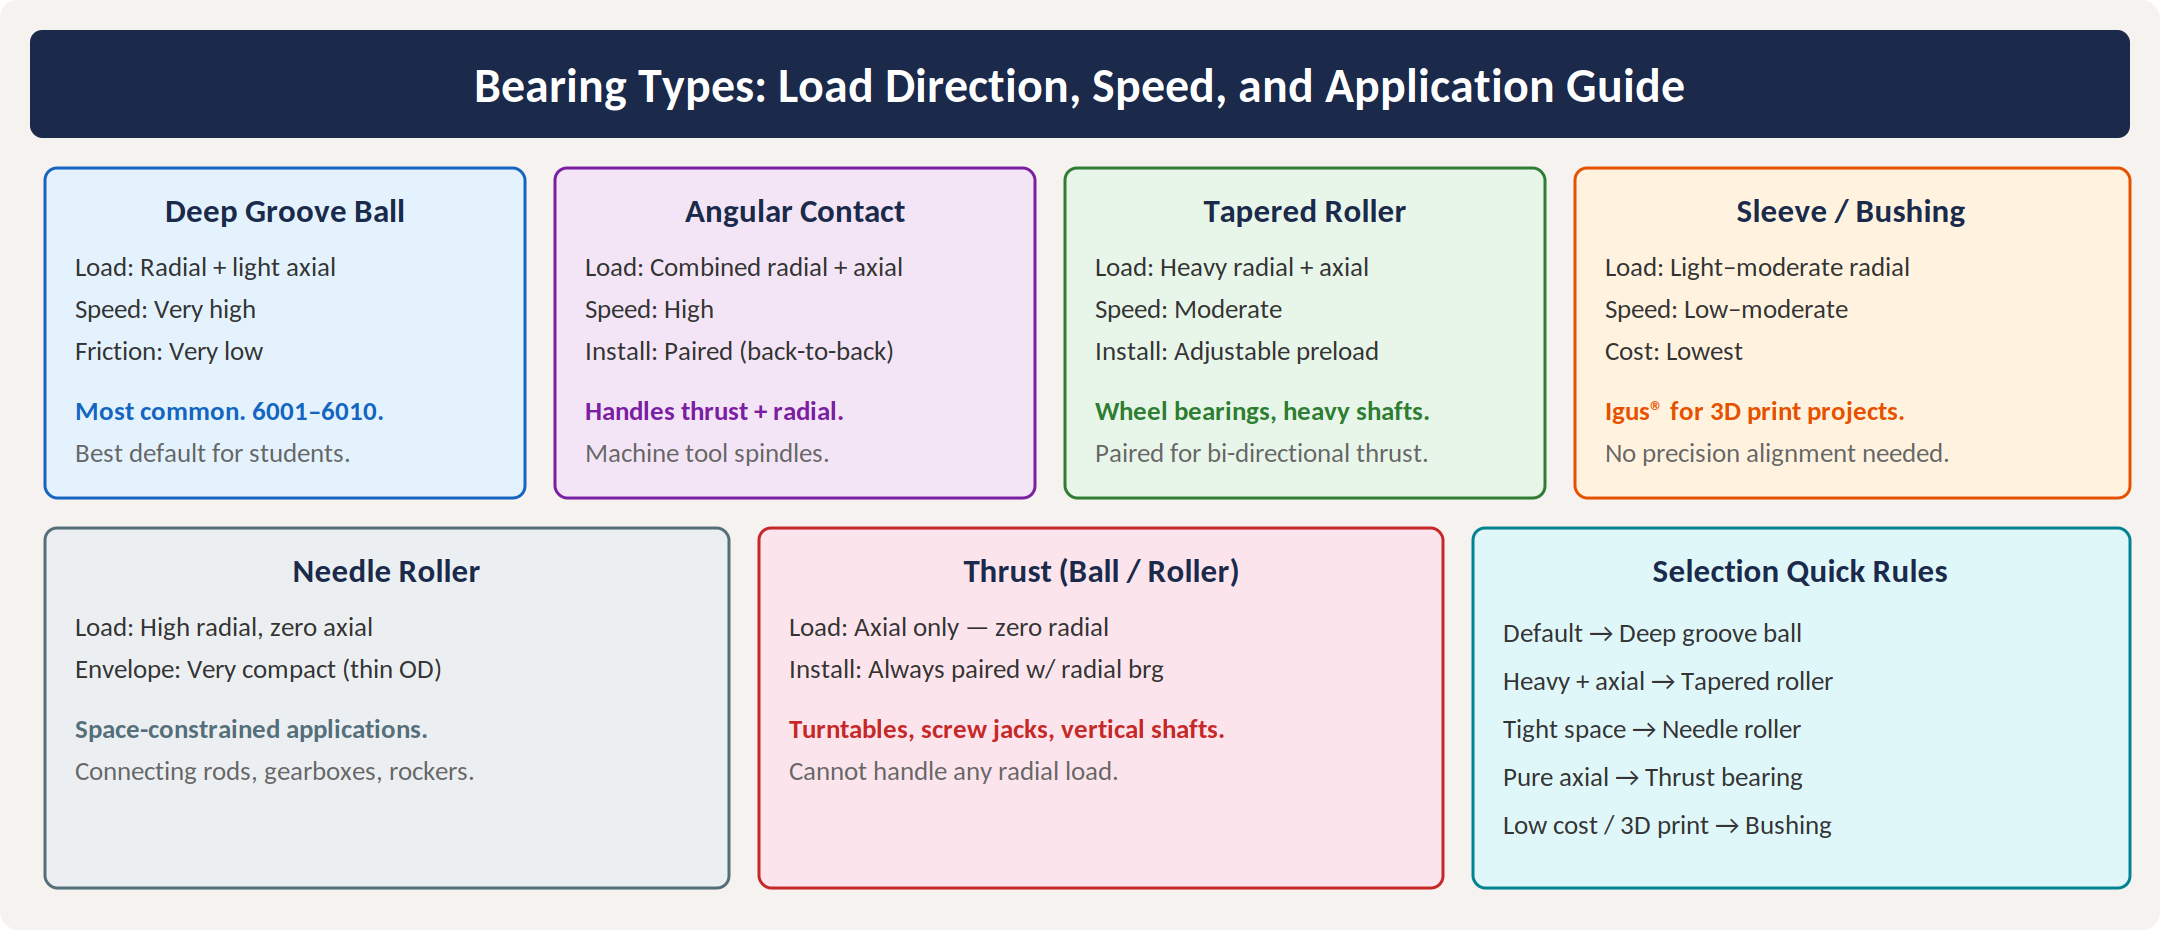
\includegraphics[width=\textwidth]{master_figs/fig_bearing_types.png}
\caption{Six bearing types with load direction, speed capability, and application guidance.}\label{fig:btypes}
\end{figure}

\textbf{Deep groove ball} (6000 series): default for students. Radial + light axial, high speed, low cost. \textbf{Angular contact}: combined radial + axial; installed in pairs. \textbf{Tapered roller}: heavy combined loads (wheel bearings). \textbf{Needle roller}: compact, high radial, zero axial. \textbf{Thrust}: axial only; always pair with a radial bearing. \textbf{Sleeve/bushing}: no rolling elements, low cost, quiet. Igus iglide\textregistered{} polymer bushings are excellent for 3D-printed housings.

\subsection{Bearing Selection}
\begin{figure}[htbp]\centering
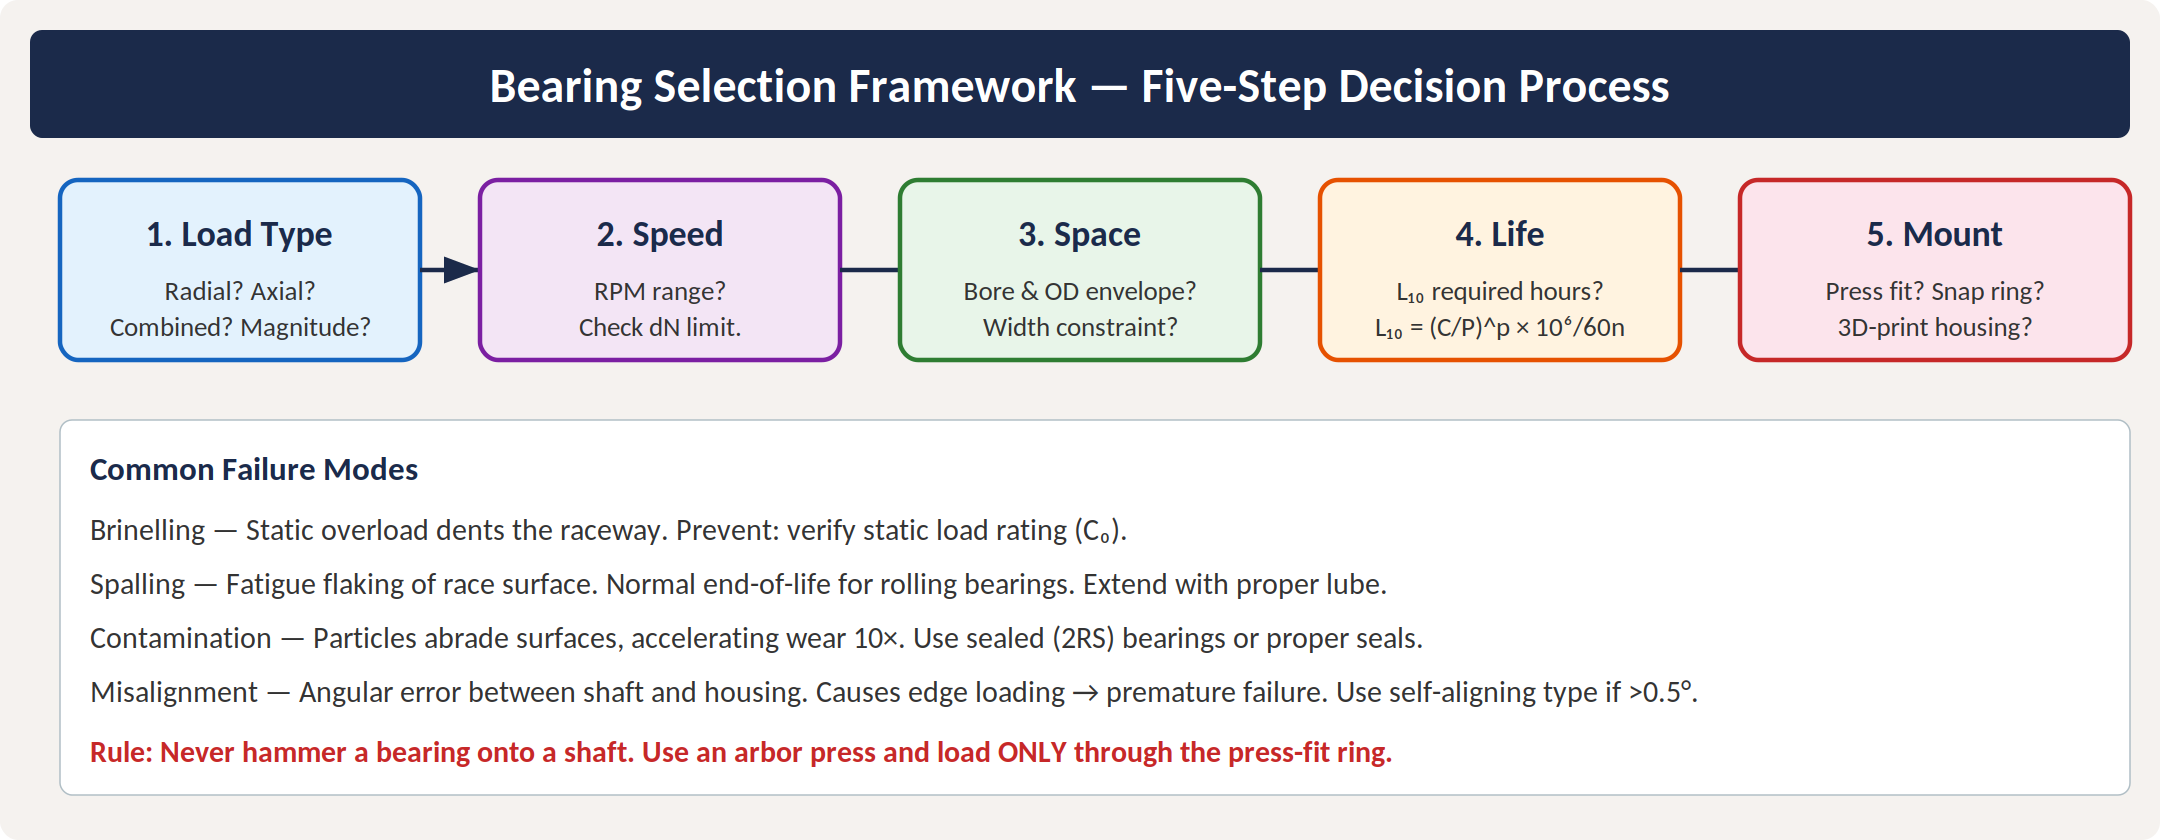
\includegraphics[width=\textwidth]{master_figs/fig_bearing_selection.png}
\caption{Five-step bearing selection framework with common failure modes.}\label{fig:bsel}
\end{figure}

Five steps: (1) \textbf{Load type and magnitude}; calculate equivalent dynamic load $P$. (2) \textbf{Speed}; check limiting RPM. (3) \textbf{Space}; bore and OD constraints. (4) \textbf{Life}; $L_{10} = (C/P)^p \times 10^6 / (60n)$ hours. (5) \textbf{Mounting}; press fit, retaining ring, adhesive.

\begin{tipbox}[Bearing Sizing for Student Projects]
(1) Select shaft diameter. (2) Look up matching bearing (8\,mm shaft $\to$ 608-2RS, \$2). (3) Verify $C \geq 3\times$ max load. (4) Order 2RS (sealed) variant. Done.
\end{tipbox}

\subsection{Mounting Bearings}
\textbf{Press fit}: bore interference fit on shaft (0.005--0.015\,mm). Use an arbor press; press only on the fitted ring.

\begin{tipbox}[Mounting Bearings in 3D Prints]
FDM tolerance $\pm$0.2--0.3\,mm. For bearing pockets: design 0.1--0.2\,mm undersize and ream to fit, or 0.05\,mm oversize with retaining compound (Loctite 638). Always test-fit with a prototype print.
\end{tipbox}

\begin{warningbox}[Never Hammer a Bearing]
Striking a bearing transmits shock through rolling elements, creating brinelling dents. These cause vibration, noise, and premature failure. Always use an arbor press or soft-jaw vise.
\end{warningbox}

\subsection{Failure Modes}
\textbf{Brinelling}: static overload dents raceway. \textbf{Spalling}: fatigue flaking (normal end-of-life). \textbf{Contamination}: particles accelerate wear $10\times$; use sealed (2RS) bearings. \textbf{Misalignment}: angular error causes edge loading.


\subsection{Thread Engagement Table}
\begin{table}[htbp]\centering\small
\begin{tabularx}{\textwidth}{l c c X}
\toprule
\textbf{Material} & \textbf{Min Engagement} & \textbf{Preferred} & \textbf{Notes} \\
\midrule
Steel & 1.0$d$ & 1.5$d$ & Standard for structural joints \\
Aluminum & 1.5$d$ & 2.0$d$ & Softer threads require more engagement \\
Cast iron & 1.5$d$ & 2.0$d$ & Brittle; threads can crack if overtorqued \\
Plastic (ABS) & 2.0$d$ & 2.5$d$ & Use coarse thread; consider threaded insert \\
Brass & 1.5$d$ & 2.0$d$ & Avoid for high-torque applications \\
\bottomrule
\end{tabularx}
\caption{Minimum thread engagement by material.}
\end{table}

\subsection{Threaded Inserts for 3D-Printed Parts}
Direct threading into FDM plastic is unreliable; the threads strip under moderate torque. Three better options: \textbf{Heat-set brass inserts} (pressed in with a soldering iron; strongest, most professional), \textbf{press-fit inserts} (pushed into undersized holes; adequate for light loads), and \textbf{captive nuts} (hex nut trapped in a designed pocket during printing). Heat-set inserts (McMaster \#94180A series) are the recommended solution for MEGN~301 projects.

\subsection{Bolt Selection Checklist}
\begin{enumerate}[nosep,leftmargin=1.5em]
\item Determine joint loads (tension, shear, or combined).
\item Select thread standard (metric for new designs).
\item Select grade/class based on load with $\geq$2$\times$ safety factor.
\item Size diameter from shear/tension calculations.
\item Determine length: grip length + nut + washer + 2--3 exposed threads.
\item Specify head type based on tool access and flush requirements.
\item Specify locking method based on vibration environment.
\item Calculate and specify torque value.
\item Add all details to BOM entry.
\end{enumerate}

\section{Design Rules of Thumb}
\begin{enumerate}[leftmargin=1.5em]
\item Thread engagement: min 1.5$d$ in steel, 2$d$ in aluminum, 2.5$d$ in plastic.
\item Bolt spacing: min 3$d$ center-to-center, 2$d$ from edge.
\item Inner ring press fit to shaft; outer ring sliding fit to housing (rotating-shaft case).
\item Always specify grade, material, finish, and torque in assembly documentation.
\end{enumerate}


\begin{keyconceptbox}[Requirements Mapping: From Fastener Specs to Shall-Statements]
Mechanical joining generates system requirements:
\begin{itemize}[nosep,leftmargin=1.5em]
\item ``Vibration environment (field deployment)'' $\to$ MECH-REQ: All structural fasteners shall use positive locking (nyloc, thread-locker, or Nord-Lock). Split washers shall not be used.
\item ``Enclosure opens for maintenance'' $\to$ MECH-REQ: Enclosure fasteners shall be captive (retained in the cover after removal) and require only a \#2 Phillips driver.
\item ``Shaft supports 50\,N radial load at 1500\,RPM'' $\to$ BRG-REQ: Shaft bearing shall have $L_{10} \geq 5000$\,hrs at the specified load and speed. Bearing type: deep-groove ball, sealed (2RS).
\end{itemize}
\end{keyconceptbox}

\section{Threaded Fastener Design}
\subsection{Bolt Sizing}
The primary design criterion for a bolted joint is the clamping force. The bolt must provide sufficient clamping force to prevent joint separation under the maximum expected external load, plus a safety factor. The clamping force is related to the tightening torque by:
\begin{equation}
T = K \cdot d \cdot F_i
\end{equation}
where $T$ is the torque, $K$ is the nut factor (approximately 0.2 for dry steel, 0.15 for lubricated), $d$ is the nominal bolt diameter, and $F_i$ is the initial clamping force (preload). For the joint to remain clamped under external load $F_{\text{ext}}$: $F_i > F_{\text{ext}} / (1 - C)$ where $C$ is the joint stiffness ratio (typically 0.1--0.3 for metal-on-metal joints).

\subsection{Thread Engagement}
The minimum thread engagement length to develop full bolt strength: for steel bolts in steel: $L_e \geq 1.0d$ (one diameter). For steel bolts in aluminum: $L_e \geq 1.5d$ (the aluminum threads are weaker). For steel bolts in plastic: $L_e \geq 2.5d$ or use threaded inserts (Heli-Coils).

\subsection{Thread Locking}
Under vibration, threaded fasteners can loosen. Prevention methods: (1) \textbf{Nylon-insert lock nuts} (Nyloc): a nylon collar in the nut provides friction that resists loosening. Effective, low cost, one-time use. (2) \textbf{Thread-locking adhesive} (Loctite): blue (242) for medium strength (removable with hand tools), red (271) for permanent (requires heat to remove). (3) \textbf{Split lock washers}: limited effectiveness; largely replaced by Nordlock wedge-locking washers. (4) \textbf{Safety wire}: for high-vibration aerospace applications (drilling the bolt head and wiring to an adjacent bolt).

\section{Bearing Selection and Installation}
\subsection{Bearing Types}
\textbf{Deep groove ball bearings}: the most common type. Support radial loads and moderate axial loads. Available in standard metric sizes (e.g., 608: 8\,mm bore, 22\,mm OD, used in skateboards and 3D printer wheels). Low friction, high speed capability.

\textbf{Angular contact ball bearings}: designed for combined radial and axial loads. Used in pairs (back-to-back or face-to-face) to support axial loads in both directions. Common in spindle applications.

\textbf{Needle roller bearings}: thin rollers provide high radial load capacity in a compact radial envelope. Used where space is limited (hinge pins, rocker arms).

\textbf{Sleeve (journal) bearings}: a plain cylindrical surface (bronze, PTFE, or polymer) with lubricant film between shaft and bearing. Simple, low cost, quiet. Adequate for low-speed, low-load applications (drawer slides, door hinges, cable pulleys).

\subsection{Bearing Sizing}
Bearings are sized by their rated life, which depends on the applied load:
\begin{equation}
L_{10} = \left(\frac{C}{P}\right)^3 \text{ (ball bearings)} \qquad L_{10} = \left(\frac{C}{P}\right)^{10/3} \text{ (roller bearings)}
\end{equation}
where $L_{10}$ is the life in millions of revolutions (90\% survival probability), $C$ is the basic dynamic load rating (from the catalog), and $P$ is the equivalent dynamic load. For a 608 bearing ($C = 3.45$\,kN) under 100\,N radial load: $L_{10} = (3450/100)^3 = 41{,}063$ million revolutions. At 1000\,RPM: this is 683,000 hours, far exceeding any project lifetime. Bearings in MEGN~301 projects are almost never load-limited; select based on size, availability, and cost.

\subsection{Bearing Installation}
Press the bearing onto the shaft by applying force to the inner ring (not the outer ring). For housing installation: press on the outer ring. Never apply force through the rolling elements (this creates dents in the raceways, called brinelling, which causes noise and premature failure). Use an arbor press with a properly sized tube that contacts only the ring being pressed. For light press fits: use a dead-blow hammer with a bearing installation tool. Apply a thin film of oil to the shaft and housing bore before installation.

\section{Design for Assembly (DfA)}
\textbf{Minimize part count}: every part that can be eliminated saves assembly time, reduces potential failure points, and simplifies inventory. Challenge every part: can it be combined with an adjacent part? Can its function be achieved by a feature of another part?

\textbf{Design for top-down assembly}: parts should assemble from one direction (typically gravity-assisted, top-down). Avoid requiring the assembler to flip, rotate, or hold the assembly in unstable orientations.

\textbf{Self-locating features}: use chamfers, tapers, and guide pins to align parts during assembly. A part that can only be assembled one way (poka-yoke) eliminates assembly errors.

\textbf{Standard hardware}: use the minimum number of fastener types and sizes. Ideally, one M3 screw size for all internal fasteners and one M5 for external/structural fasteners. This minimizes the tool kit and eliminates wrong-fastener errors.
\section{Fastener Material Selection}
\textbf{Low-carbon steel (Grade 2/SAE J429)}: the most common and cheapest fastener material. Tensile strength $\sim$510\,MPa. Adequate for most non-critical applications. Usually zinc-plated for corrosion resistance (adequate for indoor use; inadequate for outdoor or wet environments).

\textbf{Medium-carbon steel (Grade 5/SAE J429)}: quenched and tempered. Tensile strength $\sim$830\,MPa. Standard for automotive and structural applications. Three radial marks on the hex head identify Grade~5.

\textbf{Alloy steel (Grade 8/SAE J429)}: highest standard grade. Tensile strength $\sim$1040\,MPa. Six radial marks. Use when high clamping force is needed in a small bolt (e.g., mounting a motor that generates high vibration).

\textbf{Stainless steel (A2/304 and A4/316)}: corrosion resistant but lower strength than Grade 5 ($\sim$700\,MPa for A2). Non-magnetic (mostly). Use in wet environments, food equipment, and medical devices. Galling risk: stainless-on-stainless threads can cold-weld during tightening. Always use anti-seize compound (nickel-based: Permatex Nickel Anti-Seize or Loctite LB~8023) on stainless fasteners.

\textbf{Nylon and other polymers}: electrically insulating, non-marring, lightweight. Very low strength ($\sim$70\,MPa). Use for PCB mounting, panel retention, and applications where electrical isolation is required.

\section{Metric vs.\ Imperial Fasteners}
MEGN~301 uses metric fasteners exclusively (M2, M2.5, M3, M4, M5, M6, M8). Key dimensions:

\begin{itemize}[nosep,leftmargin=1.5em]
\item M3: 3.0\,mm diameter, 0.5\,mm pitch, 2.5\,mm hex socket (most common for electronics/small mechanisms)
\item M4: 4.0\,mm, 0.7\,mm pitch, 3.0\,mm hex
\item M5: 5.0\,mm, 0.8\,mm pitch, 4.0\,mm hex (structural connections)
\item M6: 6.0\,mm, 1.0\,mm pitch, 5.0\,mm hex
\end{itemize}

\textbf{Never mix metric and imperial fasteners in the same assembly}. They are not interchangeable: an M6 bolt ($6.0\times 1.0$\,mm) will cross-thread into a 1/4-20 UNC hole ($6.35\times 1.27$\,mm), destroying both threads.

\section{Threaded Insert Technology}
When bolting into soft materials (3D-printed plastic, wood, aluminum sheet), direct threading provides insufficient strength and wear resistance. Threaded inserts solve this:

\textbf{Heat-set inserts} (brass, knurled): heated with a soldering iron and pressed into a slightly undersized hole in thermoplastic. The plastic melts around the knurls and re-solidifies, creating a permanent, high-pullout-strength metal thread. Standard for 3D-printed enclosures. Use an insert tip on the soldering iron for consistent installation.

\textbf{Heli-Coil inserts} (stainless steel wire coils): installed into a tapped hole of the correct Heli-Coil drill and tap size. Create a wear-resistant thread in aluminum, magnesium, and other soft metals. Standard for aerospace and automotive repair of stripped threads.

\textbf{Press-in inserts} (brass, steel): pressed into a hole with an arbor press. The knurled exterior grips the surrounding material. Used in plastic injection-molded parts and machined assemblies.

\section{Adhesive Bonding}
When mechanical fasteners are impractical (thin materials, aesthetic requirements, vibration-sensitive joints), adhesives provide an alternative:

\textbf{Cyanoacrylate (CA, ``super glue'')}: fast cure (seconds), high shear strength ($\sim$20\,MPa), brittle. Good for: bonding small plastic parts, tacking components during assembly, and strain gauge installation. Poor gap-filling; requires intimate contact.

\textbf{Epoxy (two-part)}: slow cure (5 minutes to 24 hours depending on formulation), very high strength ($\sim$35\,MPa shear, $\sim$70\,MPa tensile), excellent gap-filling, chemical resistant. Standard structural adhesive. 5-minute epoxy is convenient but weaker than 24-hour types.

\textbf{Silicone (RTV)}: flexible, waterproof, temperature resistant ($-60$ to $+200$\,\degC{}). Low strength ($\sim$2\,MPa). Use for sealing, vibration isolation, and potting electronics. Not a structural adhesive.

\textbf{Thread-locking adhesive} (Loctite): applied to bolt threads to prevent loosening. Blue (242): medium strength, removable with hand tools. Red (271): permanent, requires heat ($\sim$250\,\degC{}) to remove. Purple (222): low strength, for small screws (M2--M6) that must be removable.

\begin{warningbox}[Adhesive Surface Preparation]
Adhesive strength depends critically on surface cleanliness. Always clean bonding surfaces with isopropanol (IPA) before applying adhesive. For metals: abrade lightly with 320-grit sandpaper, then clean with IPA. For plastics: IPA wipe only (abrasion can create micro-cracks that weaken the joint). For 3D-printed PLA: adhesion is poor on smooth surfaces; lightly sand to create mechanical interlock.
\end{warningbox}
\section{Practice Questions}
\begin{enumerate}[leftmargin=1.5em]
\item Your design uses an M8$\times$1.25 bolt in tapped aluminum. Minimum thread engagement depth? If limited to 10\,mm, is this sufficient?
\item A joint experiences severe vibration. Compare nyloc, Loctite 242, and Nord-Lock. Recommend one.
\item Your BOM lists ``1/4-20 bolt, qty 12'' with no other info. What is wrong? Rewrite it properly.
\item Select a bearing for an 8\,mm shaft at 3000\,RPM with 50\,N radial load. Specify designation, type, expected life.
\item A teammate suggests press-fitting bearings into PLA housings. Identify two problems and propose solutions.
\item Belt-driven stage idler pulley bearings grind after one week. Likely causes and diagnosis?
\item An M6 Class 8.8 bolt has proof load $\approx$16.3\,kN. Calculate torque for 75\% proof load preload ($K=0.20$).
\end{enumerate}

\subsection{Answers}
\begin{enumerate}[leftmargin=1.5em]
\item Min = 2$\times$8\,mm = 16\,mm for aluminum. 10\,mm = 1.25$d$; insufficient. Use through-bolt with nut, Heli-Coil insert, or thicker boss.
\item Nord-Lock for severe vibration with frequent disassembly. Loctite 271 (red) for permanent assembly. Nyloc for general use.
\item Missing: grade, head type, length, material/finish, torque. Correct: ``1/4-20 UNC $\times$ 1.00\,in hex cap, SAE Grade 5, zinc, qty 12. Torque: 8.0\,ft-lb with Loctite 242.''
\item 608-2RS: 8\,mm bore, 22\,mm OD. $C = 3.45$\,kN, $P = 0.05$\,kN. $L_{10} = (3.45/0.05)^3 \times 10^6/(60 \times 3000) = 918{,}000$\,hrs.
\item PLA: low HDT ($\$\sim\$$60\,\degC{}), creeps under load $\to$ pocket enlarges. Tolerance $\pm$0.2\,mm makes press fit unreliable. Fix: use PETG/nylon, ream pocket, or use retaining compound.
\item Contamination, misalignment, or open (unsealed) bearings. Diagnosis: spin by hand (gritty = contamination), check housing alignment, inspect seals. Replace with 2RS type.
\item $F = 0.75 \times 16{,}300 = 12{,}225$\,N. $T = 0.20 \times 12{,}225 \times 0.006 = 14.7$\,N$\cdot$m.
\end{enumerate}


\chapter{Mechanical Power Transmission}

\vspace{1em}

Power transmission converts motor output (torque and speed) into the motion your system needs. Every element, belt, chain, gear, shaft, linkage, lead screw, trades speed for torque (or vice versa), and every one introduces losses. Selecting the right transmission is the bridge between your electrical power budget and the mechanical work your system must perform.

\vspace{1em}

\section{Fundamental Relationships}
Three equations govern all power transmission:
\begin{align}
\text{Gear ratio:} \quad GR &= N_2/N_1 = \omega_1/\omega_2 = \tau_2/\tau_1 \\
\text{Power:} \quad P &= \tau \times \omega \\
\text{Efficiency:} \quad \eta &= P_{\text{out}}/P_{\text{in}}
\end{align}
\textbf{Speed down $\to$ torque up} by the gear ratio; power constant minus losses. Multi-stage efficiency compounds: $0.95^3 = 85.7\%$.

\section{Belt and Pulley Drives}
\subsection{V-Belts}
Wedge cross-section grips by friction. Allows slip (protects downstream). 90--95\% efficient. Requires tension adjustment.

\subsection{Timing Belts (Synchronous)}
Toothed belts mesh with toothed pulleys; no slip, positive drive. 97--99\% efficient.

\begin{tipbox}[GT2 Timing Belts for Student Projects]
GT2 profile (2\,mm pitch, 6\,mm width) is the standard for student projects, 3D printers, and hobby CNC. \$3--8/meter on Amazon. Pulleys 16--60 tooth for \$2--5. Always use flanged pulleys to prevent belt tracking.
\end{tipbox}

\subsection{Flat and Round Belts}
Flat belts on crowned pulleys for long center distances. Round belts (O-ring) for low-load, compact drives.

\section{Chain Drives}
Roller chain: positive engagement, 95--98\% efficient, high loads and shock tolerance. \#25 (1/4\,in pitch) for student projects. Minimum 17 teeth on small sprocket.

\begin{tipbox}[Chain Requires Lubrication]
Dry chain wears at $10\times$ the rate of lubricated chain. Apply chain lubricant (not WD-40) every 20--50 operating hours. A worn chain skips teeth; sudden and dangerous.
\end{tipbox}

\section{Gear Trains}

\begin{figure}[htbp]\centering
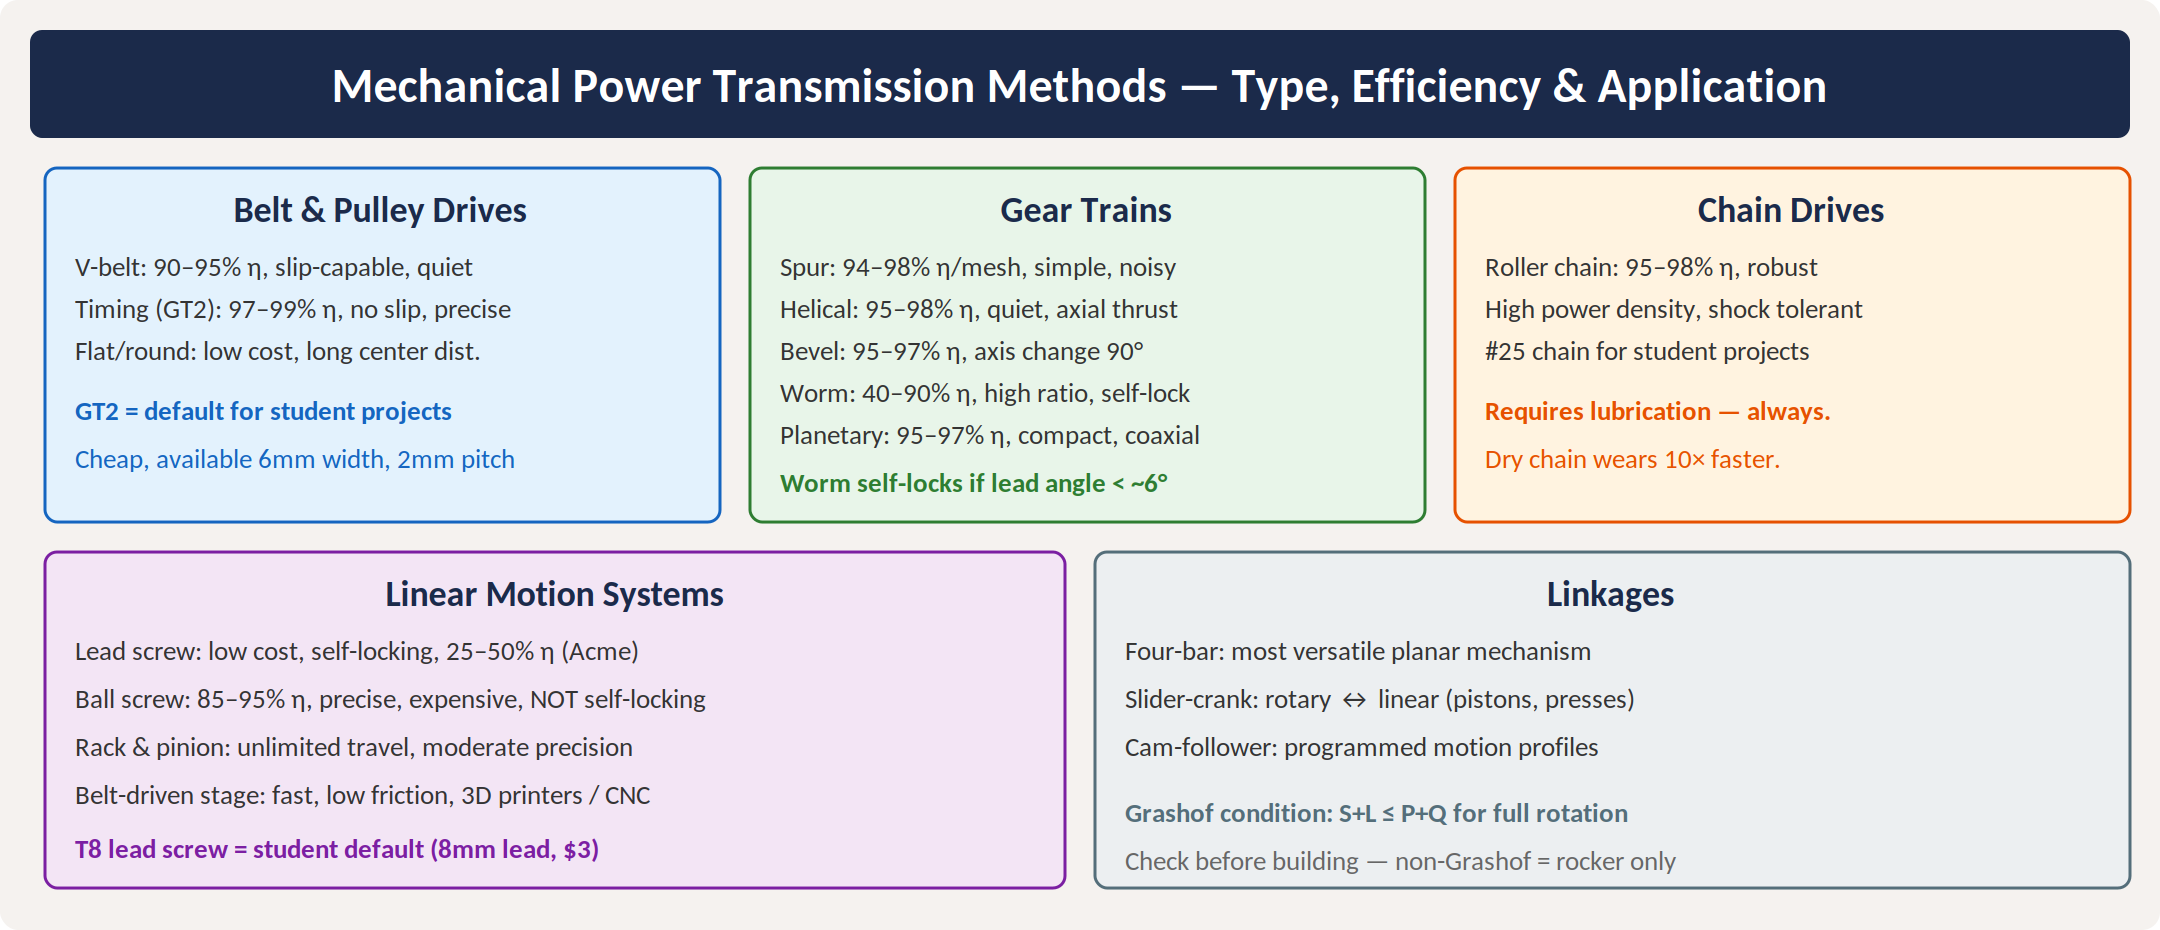
\includegraphics[width=\textwidth]{master_figs/fig_power_transmission_types.png}
\caption{Power transmission methods with efficiency, characteristics, and recommendations.}\label{fig:ptypes}
\end{figure}

\textbf{Spur}: straight teeth, 94--98\%/mesh, noisy at speed. \textbf{Helical}: angled teeth, quieter, generates axial thrust. \textbf{Bevel}: intersecting shafts (90$^{\circ}$). \textbf{Worm}: high ratio single-stage (5:1--100:1), 40--90\% efficient, \textbf{self-locking} when lead angle $<$$\$\sim\$$\ang{6}. \textbf{Planetary}: compact, coaxial, 95--97\%/stage.

\begin{tipbox}[Gear Selection for Student Projects]
ServoCity (servocity.com) sells matched spur gear sets with standardized shafts and hubs. McMaster has individual gears in any size. For 3D-printed gears: PETG or nylon, module $\geq$1.5, add 0.1--0.2\,mm backlash.
\end{tipbox}


\subsection{Gear Train Design Process}
\begin{enumerate}[nosep,leftmargin=1.5em]
\item Calculate required output torque and speed from the load.
\item Calculate gear ratio: $GR = \omega_{motor} / \omega_{load}$.
\item Select gear type based on noise, efficiency, and axis orientation requirements.
\item If $GR > 10$: use multi-stage (two spur stages) or single-stage worm/planetary.
\item Size gears for tooth bending stress and surface contact stress (Lewis equation for bending: $\sigma = W_t / (b \cdot m \cdot Y)$).
\item For student projects: select stock gears from ServoCity or McMaster and verify that the rated torque exceeds your load with $\geq$2$\times$ margin.
\item Specify mounting: shaft diameter, key or set screw, bearing supports, and housing.
\end{enumerate}

\subsection{Backlash and Precision}
Backlash is the angular play between mating gear teeth (or belt-pulley engagement). It causes positioning error and control-loop instability. Standard spur gears have 0.05--0.10\,mm backlash. For precision applications: use anti-backlash gears (split gear with spring preload), ball screws (inherently low backlash), or harmonic drives (zero backlash). For most MEGN~301 projects, standard backlash is acceptable.

\section{Shafts and Couplings}
\subsection{Shaft Design}
Shafts transmit torque and support rotating components. Default: 1045 steel. Size for torque with safety factor. Keyways add $\$\sim\$$25\% stress concentration.

\subsection{Shaft-Hub Connections}
\textbf{Keyway}: rectangular key transmits torque; standard sizes from ANSI B17.1. \textbf{Set screw}: clamps hub to flat; low torque, adequate for light student loads. \textbf{D-shaft}: flat on shaft engages matching hub flat; common on stepper motors.

\subsection{Couplings}
\textbf{Rigid}: zero misalignment tolerance. \textbf{Flexible}: jaw coupling (elastomer spider, shock absorption), beam coupling (zero backlash), Oldham (parallel offset), universal joint (large angles).

\section{Linear Motion}
\subsection{Lead Screws}
Acme-thread, 25--50\% efficient, \textbf{self-locking}. T8$\times$8 (8\,mm dia, 8\,mm lead) is the student default (\$3--8 with brass nut).

\subsection{Ball Screws}
Recirculating balls, 85--95\% efficient, precise, \textbf{not self-locking}. More expensive.

\subsection{Rack and Pinion}
Unlimited travel, moderate precision. Force = torque / pinion pitch radius.

\subsection{Belt-Driven Linear Stages}
Timing belt on two pulleys, carriage on linear rails. Fast, low friction. GT2 + MGN12 rail for student projects.

\section{Linkages}
\textbf{Four-bar}: most versatile planar mechanism. Grashof condition: $S + L \leq P + Q$ for full rotation. \textbf{Slider-crank}: rotary $\leftrightarrow$ linear (pistons, presses). Stroke = $2\times$ crank radius. \textbf{Cam-follower}: programmed motion profiles from cam shape.

\section{Selection Framework}
\begin{figure}[htbp]\centering
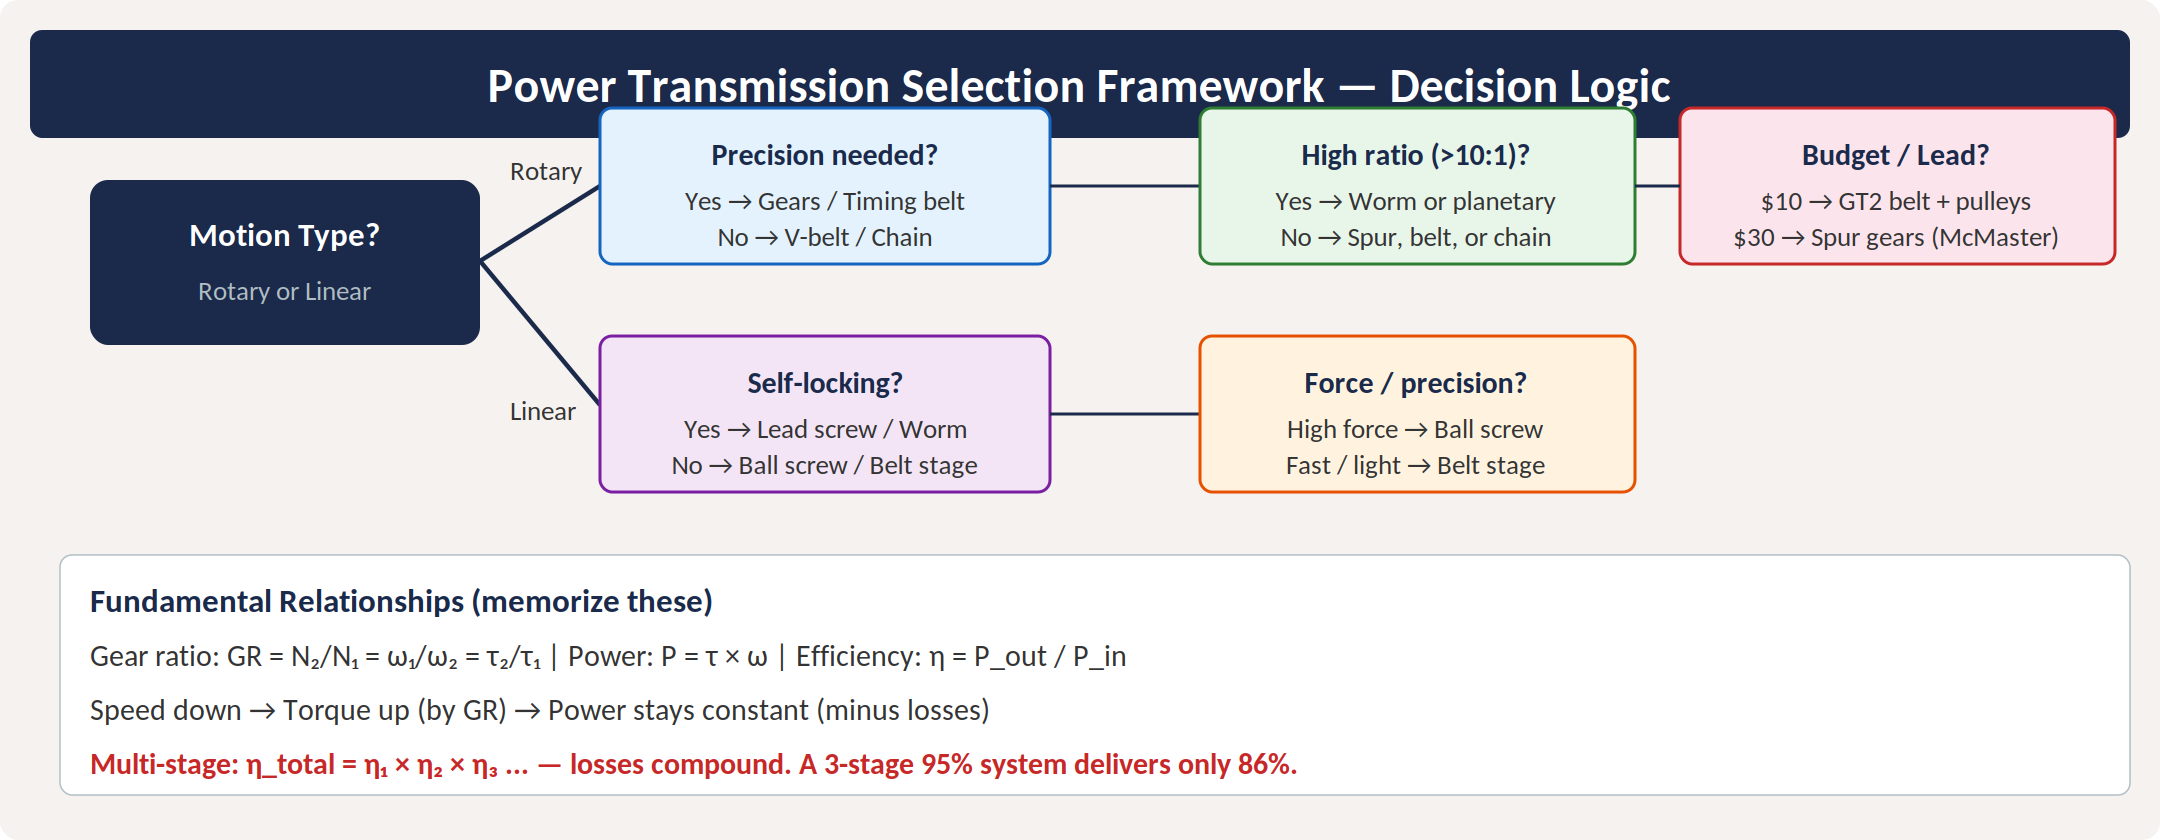
\includegraphics[width=\textwidth]{master_figs/fig_power_trans_selection.png}
\caption{Power transmission selection: motion type, precision, self-locking, ratio, budget.}\label{fig:ptsel}
\end{figure}

\begin{keyconceptbox}[Five Key Takeaways]
\begin{enumerate}[nosep,leftmargin=1.5em]
\item Speed down = torque up. Calculate output torque before selecting transmission.
\item GT2 belts and T8 lead screws are student defaults. Start there.
\item Efficiency compounds multiplicatively. Minimize stages.
\item Self-locking (lead screws, worms) holds position without power. Non-self-locking (ball screws, spur gears) needs a brake.
\item Every rotating joint needs a bearing. Every coupling needs defined misalignment tolerance.
\end{enumerate}
\end{keyconceptbox}


\begin{keyconceptbox}[Requirements Mapping: From Transmission Specs to Shall-Statements]
Power transmission design generates system requirements:
\begin{itemize}[nosep,leftmargin=1.5em]
\item ``Linear stage positions to $\pm$0.1\,mm'' $\to$ MECH-REQ: Lead screw shall have $\leq$0.05\,mm backlash. Anti-backlash nut required.
\item ``System holds position when unpowered'' $\to$ MECH-REQ: Transmission shall be self-locking (lead screw or worm gear with lead angle $<$\ang{6}).
\item ``Gear ratio 10:1 in minimum space'' $\to$ MECH-REQ: Use planetary gearbox ($\leq$40\,mm diameter) with $\geq$95\% efficiency per stage.
\end{itemize}
Calculate the required output torque and speed \emph{from requirements} before selecting any transmission hardware.
\end{keyconceptbox}

\section{Power Transmission Fundamentals}
Mechanical power transmission converts the motor's output (speed and torque at the motor shaft) into the required speed and torque at the load. The fundamental relationship:
\begin{equation}
P = T \cdot \omega
\end{equation}
where $P$ is power (W), $T$ is torque (N$\cdot$m), and $\omega$ is angular velocity (rad/s). Power is conserved (minus friction losses), so reducing speed increases torque proportionally: $T_{\text{out}} = T_{\text{in}} \times (N_{\text{in}}/N_{\text{out}}) \times \eta$ where $\eta$ is the efficiency.

\section{Gear Trains}
\subsection{Spur Gears}
The most common gear type for parallel shafts. Gear ratio: $i = N_2/N_1 = d_2/d_1$ where $N$ is the number of teeth and $d$ is the pitch diameter. For a 20-tooth pinion driving a 60-tooth gear: $i = 3$, meaning the output speed is $1/3$ of the input and the output torque is $3\times$ the input (minus friction).

\textbf{Module (metric)} or \textbf{diametral pitch (imperial)} defines the tooth size: module $m = d/N$ (mm). Common modules for small mechanisms: 0.5, 1.0, 1.5, 2.0\,mm. Both gears in a mesh must have the same module.

\textbf{Pressure angle}: typically 20\degC{} (standard). The 14.5\degC{} pressure angle is obsolete but still encountered on legacy equipment. Do not mesh gears with different pressure angles.

\textbf{Backlash}: the clearance between mating gear teeth. Necessary for thermal expansion and lubrication, but introduces positioning error. For precision applications, use anti-backlash gears (split gears with spring preload) or zero-backlash harmonic drives.

\subsection{Compound Gear Trains}
For large speed reductions ($i > 10$), use multiple stages. A two-stage train with $i_1 = 5$ and $i_2 = 4$ gives total $i = 20$ with two compact stages rather than one impractically large gear. Planetary gear sets achieve ratios of 3--10 in a single compact stage and are used in servo drives, cordless tool transmissions, and automotive automatic transmissions.

\section{Belt and Chain Drives}
\textbf{Timing belts} (synchronous belts): positive engagement (no slip). Tooth profiles: GT2 (2\,mm pitch, standard for 3D printers and small mechanisms), HTD (higher torque capacity for larger systems). Advantages: precise speed ratio, no lubrication, quiet. Sizing: select belt width for the required torque; the belt manufacturer's catalog provides power ratings per unit width for each tooth profile.

\textbf{V-belts}: friction drive (slight slip under load). Simple, tolerant of misalignment, absorbs vibration. Used in industrial machinery, HVAC, and automotive accessories. Not suitable for precise positioning.

\textbf{Roller chain}: positive engagement, high torque capacity. Standard sizes: \#25 (1/4-inch pitch), \#35 (3/8-inch), \#40 (1/2-inch). Requires lubrication and tensioning. Noisy at high speed. Used in bicycles, motorcycles, and industrial conveyors.

\section{Lead Screws and Linear Motion}
Converting rotary motion to linear motion:

\textbf{Lead screws}: a threaded rod turns in a nut, translating rotary motion to linear motion. The lead $l$ (linear distance per revolution) determines the speed and force: $v = l \cdot n$ (speed), $F = 2\pi T/(l \cdot \eta)$ (force). Standard trapezoidal (ACME) thread: $\eta \approx 40\%$. Ball screws (recirculating ball bearings in the nut): $\eta \approx 90\%$, but 10$\times$ the cost.

\textbf{Rack and pinion}: a spur gear (pinion) meshes with a linear gear (rack). Linear speed $= \pi d n$ where $d$ is the pinion pitch diameter. Used in CNC machines, steering systems, and linear actuators.

\section{Coupling Selection}
Couplings connect two shafts and transmit torque. They must accommodate misalignment between the shafts:

\textbf{Rigid couplings}: no misalignment tolerance. Used only when shafts are precisely aligned (lathe spindles, precision instruments). Types: sleeve, clamp, keyed.

\textbf{Flexible couplings}: accommodate angular, parallel, and axial misalignment. Types: jaw (elastomer insert absorbs vibration; most common in student projects), beam (single-piece helical cut; allows angular and axial flex), Oldham (sliding disk; accommodates parallel offset), and universal joint (large angular misalignment for non-parallel shafts).

\textbf{Selection criteria}: (1) torque rating $\geq 2\times$ the maximum torque (safety factor for shock loads), (2) bore size matches both shafts, (3) misalignment tolerance $\geq$ the expected misalignment (typically $\pm$1\degC{} angular and $\pm$0.5\,mm parallel for student assemblies), (4) set screw or clamp style (clamp is preferred; set screws can loosen and damage the shaft).

\section{Efficiency and Heat Generation}
Every transmission element converts some input power to heat through friction. Typical efficiencies: spur gears 95--98\% per stage, timing belt 95--98\%, roller chain 95--98\%, V-belt 90--95\%, worm gear 40--90\% (depending on ratio), lead screw 30--50\% (ACME), ball screw 85--95\%.

For a two-stage spur gear train driving a lead screw: $\eta_{\text{total}} = 0.97 \times 0.97 \times 0.40 = 0.376$ (37.6\%). A 10\,W motor delivers only 3.76\,W to the load; 6.24\,W is dissipated as heat in the gear teeth and screw thread. This heat must be managed (lubrication, heat sinking, duty cycle limits) or the mechanism will overheat and seize.
\section{Gear Design for 3D-Printed Prototypes}
3D printing enables rapid prototyping of custom gears, but the material properties and dimensional accuracy impose limitations:

\textbf{FDM (PLA, ABS, PETG)}: layer lines on tooth flanks increase friction and noise. Typical tolerance: $\pm$0.2\,mm, which limits the minimum module to $m \geq 1.5$\,mm (smaller teeth do not print accurately). Tooth strength is limited by the layer adhesion (Z-direction strength is 30--70\% of XY strength). Print gears with teeth oriented in the XY plane for maximum strength. Expect 50--100 hours of operation before significant wear; suitable for proof-of-concept but not production.

\textbf{SLA (resin)}: much finer detail (tolerance $\pm$0.05\,mm), enabling module $\geq 0.5$\,mm. Smoother tooth surfaces reduce friction. However, standard SLA resins are brittle; use tough or engineering resins for functional gears. UV degradation limits outdoor use.

\textbf{Design tips}: (1) increase backlash to $1.5\times$ the standard value to accommodate print tolerance, (2) add a 0.5\,mm fillet at the tooth root to reduce stress concentration (which FDM's layer structure amplifies), (3) print a test gear pair and verify meshing before printing the full mechanism.

\section{Motor-to-Load Matching}
The motor must be selected to match the load's torque and speed requirements through the transmission. The design procedure:

\textbf{Step 1}: determine the load requirements at the output shaft. What torque ($T_{\text{load}}$) and speed ($n_{\text{load}}$) does the application need?

\textbf{Step 2}: select a gear ratio. $i = n_{\text{motor}}/n_{\text{load}}$. The motor's rated speed is typically 3000--12{,}000\,RPM; the load speed is often 10--500\,RPM.

\textbf{Step 3}: calculate the motor torque requirement. $T_{\text{motor}} = T_{\text{load}} / (i \times \eta)$ where $\eta$ is the transmission efficiency.

\textbf{Step 4}: select a motor whose rated torque exceeds $T_{\text{motor}}$ with a safety factor of $\geq 1.5$. Also verify that the motor's rated speed matches $n_{\text{load}} \times i$.

\textbf{Step 5}: verify the power. $P_{\text{motor}} = T_{\text{motor}} \times \omega_{\text{motor}} \geq T_{\text{load}} \times \omega_{\text{load}} / \eta$.

\begin{greenshieldbox}[GreenShield: Motor Selection for a Pump Drive]
The pump requires $T_{\text{load}} = 0.3$\,N$\cdot$m at $n_{\text{load}} = 300$\,RPM. Using a 2-stage spur gear reduction with $i = 10$ and $\eta = 0.94$: $T_{\text{motor}} = 0.3/(10 \times 0.94) = 0.032$\,N$\cdot$m at $n_{\text{motor}} = 3000$\,RPM. Power: $P = 0.3 \times 300 \times 2\pi/60 = 9.4$\,W. Select a motor rated for $\geq 0.048$\,N$\cdot$m (1.5$\times$ safety factor) at 3000\,RPM, with $\geq 15$\,W power rating. A typical 12\,V, 380-size brushed DC motor meets these requirements.
\end{greenshieldbox}

\section{Linear Actuator Design}
For applications requiring linear force (clamping, pressing, positioning), convert rotary motor output to linear motion:

\textbf{Lead screw actuator}: motor $\to$ coupling $\to$ lead screw $\to$ nut. Linear speed $v = l \times n$ (lead $\times$ RPM). Force $F = 2\pi T_{\text{motor}} \times i / l \times \eta$. Self-locking when the lead angle $< \arctan(\mu)$ (typically $< 5$\degC{}), meaning the load cannot back-drive the motor. This is useful for holding position without power.

\textbf{Belt-driven linear stage}: motor $\to$ timing pulley $\to$ belt $\to$ carriage. Linear speed $v = \pi d n$ (pulley diameter $\times$ RPM). Not self-locking; the carriage moves freely when the motor is unpowered (use a brake or worm gear if holding is needed). Very fast: typical belt-driven CNC axes achieve 200--500\,mm/s.

\textbf{Rack and pinion}: motor $\to$ pinion gear $\to$ rack. Linear speed $v = \pi d n$. Compact, high force, bidirectional. Common in CNC routers and industrial automation.

\section{Vibration and Noise in Power Transmission}
Gear noise arises from tooth meshing: each tooth engagement creates a brief impulse that excites structural resonances. Noise is proportional to speed, load, and gear quality. Mitigation: (1) use helical gears instead of spur (gradual engagement reduces impact), (2) increase gear quality grade (AGMA 8 or higher), (3) use plastic or composite gears for light loads (inherent damping reduces noise), (4) enclose the gear train in a housing with vibration-damping mounts.

Belt drives are inherently quieter than gears (flexible belt absorbs vibration). Chain drives are the noisiest (metal-on-metal impact at each link engagement). For noise-sensitive applications (laboratory instruments, medical devices, consumer products): use timing belts or direct drive (no transmission, oversized motor at the load speed).
\begin{keyconceptbox}[Requirements Mapping: Power Transmission]
\textbf{From technical specs to ``shall'' statements:}

A timing belt drive using a GT2 belt with a 20-tooth pulley ($d = 12.73$\,mm) at 3000\,RPM produces linear speed $v = \pi \times 0.01273 \times 3000/60 = 2.0$\,m/s. This becomes: ``SYS-SPD-001: The linear stage shall achieve a travel speed of $2.0 \pm 0.1$\,m/s. \emph{Verification: Test --- measure travel time over 500\,mm using a stopwatch ($N = 10$ trials).}''

A two-stage gear train ($i = 20$, $\eta = 0.94$) with a motor rated at 0.05\,N$\cdot$m delivers $0.05 \times 20 \times 0.94 = 0.94$\,N$\cdot$m at the output. This becomes: ``SYS-TRQ-001: The output shaft shall deliver $\geq 0.9$\,N$\cdot$m at 150\,RPM. \emph{Verification: Test --- measure stall torque with a spring scale at a known radius.}''
\end{keyconceptbox}
\section{Practice Questions}
\begin{enumerate}[leftmargin=1.5em]
\item A NEMA~17 stepper produces 0.4\,N$\cdot$m at 200\,RPM. You need 2.0\,N$\cdot$m at 40\,RPM. What gear ratio is required? What efficiency must the transmission achieve?
\item Compare GT2 timing belt vs.\ roller chain for a 3:1 reduction on a small conveyor. Which do you choose and why?
\item Your linear stage uses a T8$\times$8 lead screw driven by a stepper at 200\,RPM. Calculate the linear speed in mm/s. If the stage must move 200\,mm, how long does the motion take?
\item A worm gear set has a 30:1 ratio and 60\% efficiency. Input power is 50\,W. What is the output power? Is this set self-locking?
\item Your project needs a mechanism that converts continuous motor rotation into a back-and-forth linear stroke of 50\,mm. Propose two different mechanism solutions and compare them.
\item A 4-bar linkage has link lengths 40, 100, 70, and 80\,mm. Check the Grashof condition. Which link(s) can make a full revolution?
\item Your belt-driven linear stage stalls under load. The stepper motor skips steps but does not overheat. Diagnose the root cause and propose fixes.
\end{enumerate}

\subsection{Answers}
\begin{enumerate}[leftmargin=1.5em]
\item $GR = 2.0/0.4 = 5:1$ (or $200/40 = 5:1$). Check: $P_{in} = 0.4 \times (200 \times 2\pi/60) = 8.38$\,W. $P_{out} = 2.0 \times (40 \times 2\pi/60) = 8.38$\,W for 100\% efficiency. With real losses, the transmission must be $\geq$100\% to deliver full torque; meaning the motor is marginally sized. Derate: need $\geq$85\% efficient transmission (GT2 belt: 97\%, spur gear: 94\% work; worm at 60\% does not).
\item GT2 belt: no lubrication, clean, quiet, 97\% efficient, \$10 total. Chain: requires lube, messy, noisier, 96\% efficient, \$15. For a small indoor conveyor, GT2 wins on cleanliness, cost, and simplicity. Chain is better if the conveyor sees high shock loads or outdoor contamination.
\item Linear speed = lead $\times$ RPM / 60 = 8\,mm $\times$ 200/60 = 26.7\,mm/s. Time = 200/26.7 = 7.5\,s.
\item $P_{out} = 50 \times 0.60 = 30$\,W. At 30:1 ratio, the lead angle is very low ($\ll$\ang{6}), so yes; self-locking.
\item (a) Slider-crank: crank radius = 25\,mm, continuous rotation $\to$ 50\,mm stroke. Simple, constant stroke. (b) Belt-driven stage with limit switches: motor reverses at each end. Variable stroke and speed via firmware. Slider-crank is simpler mechanically; belt stage is more flexible.
\item $S = 40, L = 100, P = 70, Q = 80$. $S + L = 140$. $P + Q = 150$. $140 \leq 150$. Grashof satisfied. The shortest link (40\,mm) can make full revolution. If grounded, it is the crank.
\item Motor torque is sufficient (no overheating) but the belt/pulley system cannot transmit the load. Causes: belt tension too low (belt slips on pulley teeth), pulley set screw loose (pulley spins on shaft), or load exceeds belt rating. Fixes: increase belt tension, verify set screws, check that belt width and tooth count match the load.
\end{enumerate}

\chapter{Designing for Injection Molding}

\vspace{1em}




\vspace{1em}


% ══════════════════════════════════════════════════════════════════════
\section{Injection Molding Fundamentals}
% ══════════════════════════════════════════════════════════════════════

\subsection{Process Overview}

Injection molding produces plastic parts by forcing molten thermoplastic into a precision steel mold under high pressure. The machine has two units: the \textbf{injection unit} (barrel, screw, heater bands, nozzle) melts pellets and injects them, and the \textbf{clamping unit} (platens, tie bars, hydraulic or toggle mechanism) holds the mold closed. Machines are rated by clamp force (tons) and shot size (oz or g).

The mold has two halves: the \textbf{cavity} (A-side, stationary, forms the outside/cosmetic surface) and the \textbf{core} (B-side, moving, forms the inside surface). The \textbf{parting line} is where the halves meet. Inside the mold, a \textbf{runner system} distributes melt from the nozzle to the gate, \textbf{cooling channels} extract heat, and \textbf{ejector pins} push the part out.

\subsection{The Four-Phase Cycle}

\begin{figure}[htbp]
\centering
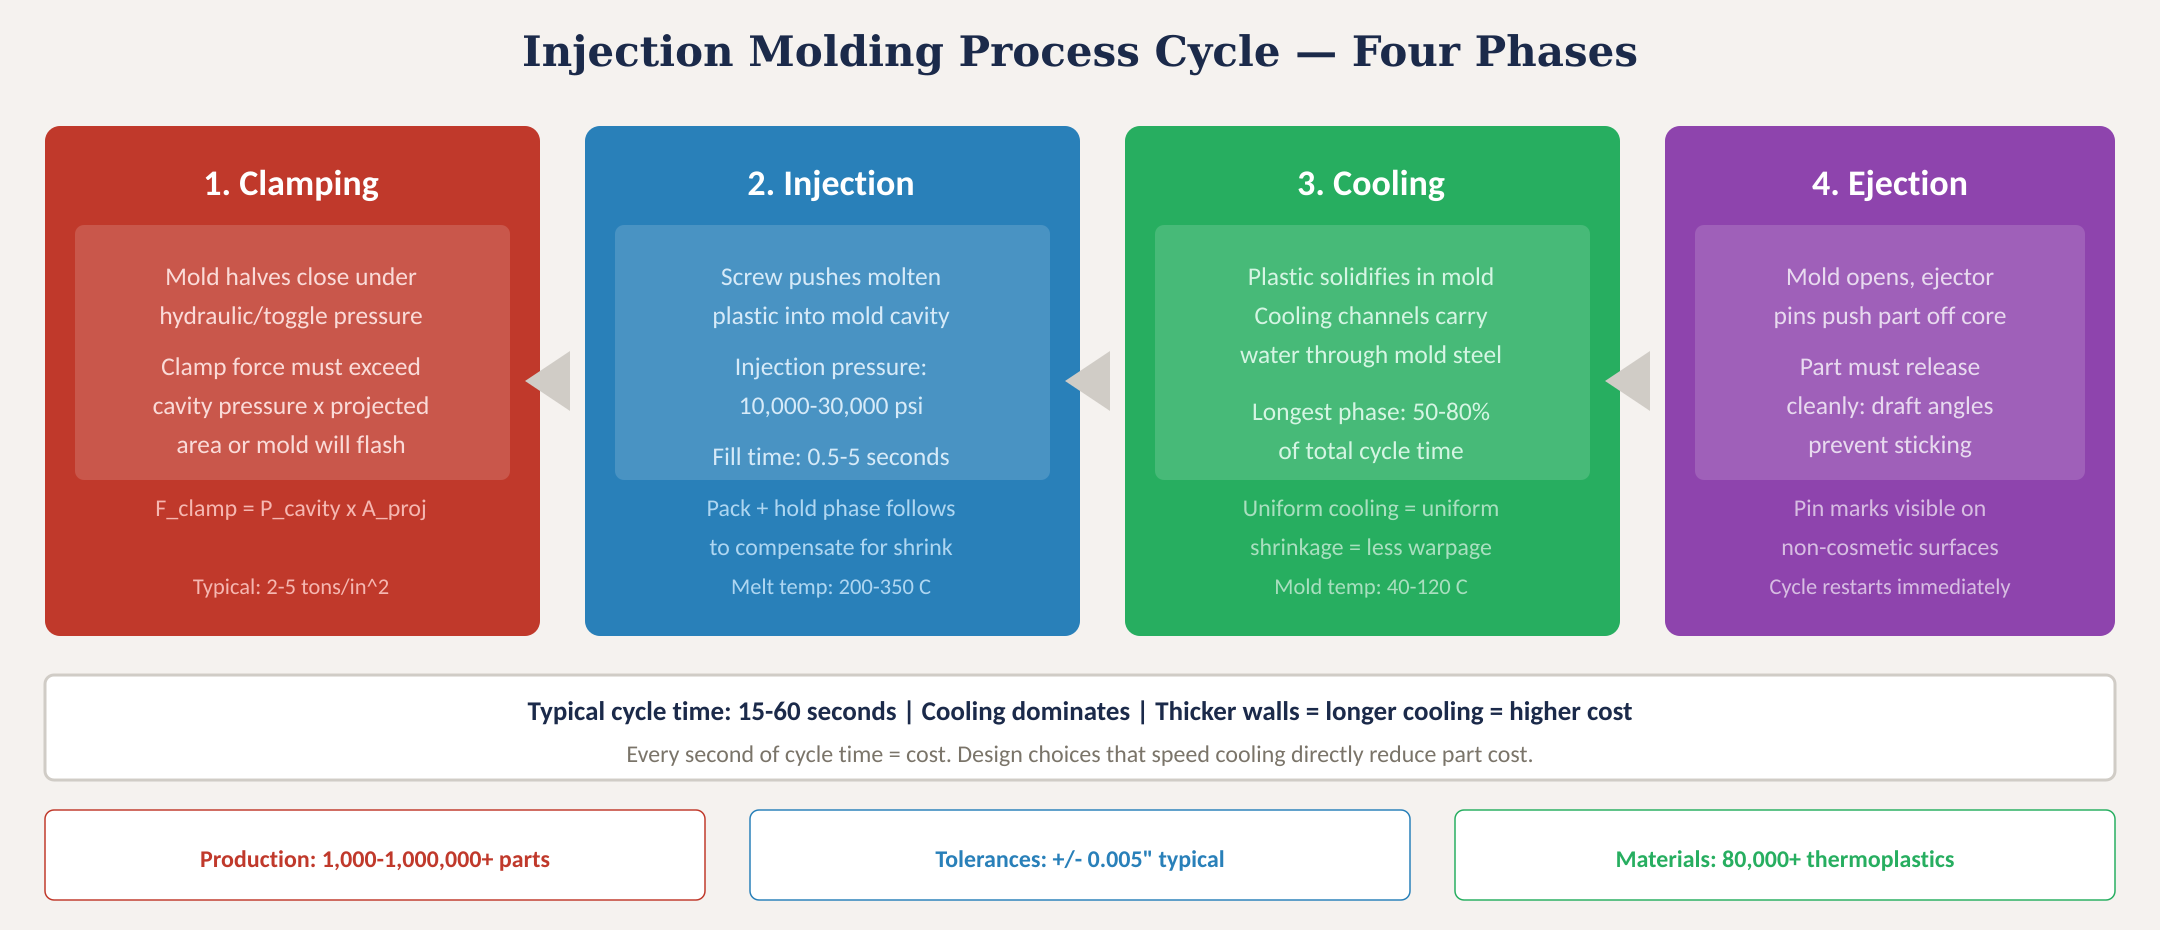
\includegraphics[width=\textwidth]{master_figs/fig_process_cycle.png}
\caption{Four-phase injection molding cycle with process parameters, timing, and production capabilities.}
\label{fig:cycle}
\end{figure}

\begin{enumerate}[leftmargin=1.5em]
  \item \textbf{Clamping}: Mold halves close under force. Required clamp force:
  \begin{equation}
    F_{\text{clamp}} = P_{\text{cavity}} \times A_{\text{projected}}
  \end{equation}
  Typical cavity pressures: 2--5~tons/in$^2$. A part with 10~in$^2$ projected area needs 20--50 tons of clamp force.

  \item \textbf{Injection}: The screw pushes molten plastic into the cavity at 10,000--30,000~psi. Fill time: 0.5--5~seconds. A \textbf{pack-and-hold} phase follows to compensate for volumetric shrinkage as the plastic cools. Without adequate packing, parts have sink marks and are undersized. Melt temperatures range from 200\,$^{\circ}$C (PE) to 350\,$^{\circ}$C (PC, nylon).

  \item \textbf{Cooling}: Plastic solidifies in the mold. This is the \textbf{longest phase}: 50--80\% of total cycle time. Cooling water flowing through channels in the mold steel extracts heat. \textbf{Uniform cooling = uniform shrinkage = minimal warpage.} Mold temperatures: 40--120\,\degC{} depending on material. Cooling time scales with the \emph{square} of wall thickness; doubling wall thickness quadruples cooling time.

  \item \textbf{Ejection}: Mold opens, ejector pins push part off the core. Part must have \textbf{draft angles} so it releases cleanly. Pin marks are visible on non-cosmetic (B-side) surfaces. The cycle restarts immediately.
\end{enumerate}

\begin{warningbox}[Cycle Time = Cost]
Typical total cycle: 15--60~seconds. Every additional second of cycle time increases part cost. Wall thickness is the primary driver; every millimeter of additional wall can add 5--15~seconds of cooling per cycle. Design the thinnest wall that meets structural and flow requirements.
\end{warningbox}


\subsection{Material Selection}
\label{sec:materials}

\begin{table}[htbp]
\centering\small
\begin{tabularx}{\textwidth}{l l X c l}
  \toprule
  \textbf{Material} & \textbf{Trade Names} & \textbf{Key Properties} & \textbf{Shrink} & \textbf{Common Uses} \\
  \midrule
  ABS & Cycolac & Good impact, easy to mold/paint, 80\,\degC & 0.5--0.7\% & Enclosures, LEGO \\
  PC & Lexan & High impact, optical clarity, 130\,\degC, UV-sensitive & 0.5--0.7\% & Lenses, phone cases \\
  PP & Pro-fax & Chemical resistant, living hinge, low cost & 1.0--2.5\% & Containers, caps \\
  Nylon (PA) & Zytel & High strength/stiffness, absorbs moisture & 0.8--1.5\% & Gears, connectors \\
  POM & Delrin & Low friction, dimensional stability, fatigue & 1.8--2.5\% & Gears, zippers \\
  PC/ABS & Bayblend & PC toughness + ABS processability & 0.5--0.7\% & Laptops, power tools \\
  PBT & Valox & Good electrical, chemical resistant & 1.5--2.0\% & Electrical connectors \\
  TPE/TPU & Santoprene & Flexible, rubber-like, overmoldable & 0.5--2.0\% & Grips, seals \\
  \bottomrule
\end{tabularx}
\caption{Common injection molding thermoplastics.}
\end{table}

\textbf{Selection criteria}: Match the \emph{cheapest} material that satisfies all of the following; mechanical loads (tensile, impact, flex), thermal environment (HDT, continuous use temperature, UL94 flammability), chemical exposure (solvents, UV, oils), aesthetics (gloss, texture, transparency, paintability), and processing (MFI, shrinkage, moisture sensitivity). Glass-fiber reinforcement increases stiffness 2--3$\times$ but reduces impact and abrades the mold.

\begin{tipbox}[Shrinkage Matters]
When hot plastic cools it contracts. The mold cavity is cut \emph{larger} than the finished part by the shrinkage factor. High-shrinkage materials (PP at 1--2.5\%) require more generous tolerances than low-shrinkage materials (ABS at 0.5--0.7\%). Crystalline polymers (PP, nylon, POM) shrink more than amorphous ones (ABS, PC, PS).
\end{tipbox}


% ══════════════════════════════════════════════════════════════════════
\section{Design for Manufacturing (DFM) Rules}
\label{sec:dfm}
% ══════════════════════════════════════════════════════════════════════

\begin{figure}[htbp]
\centering
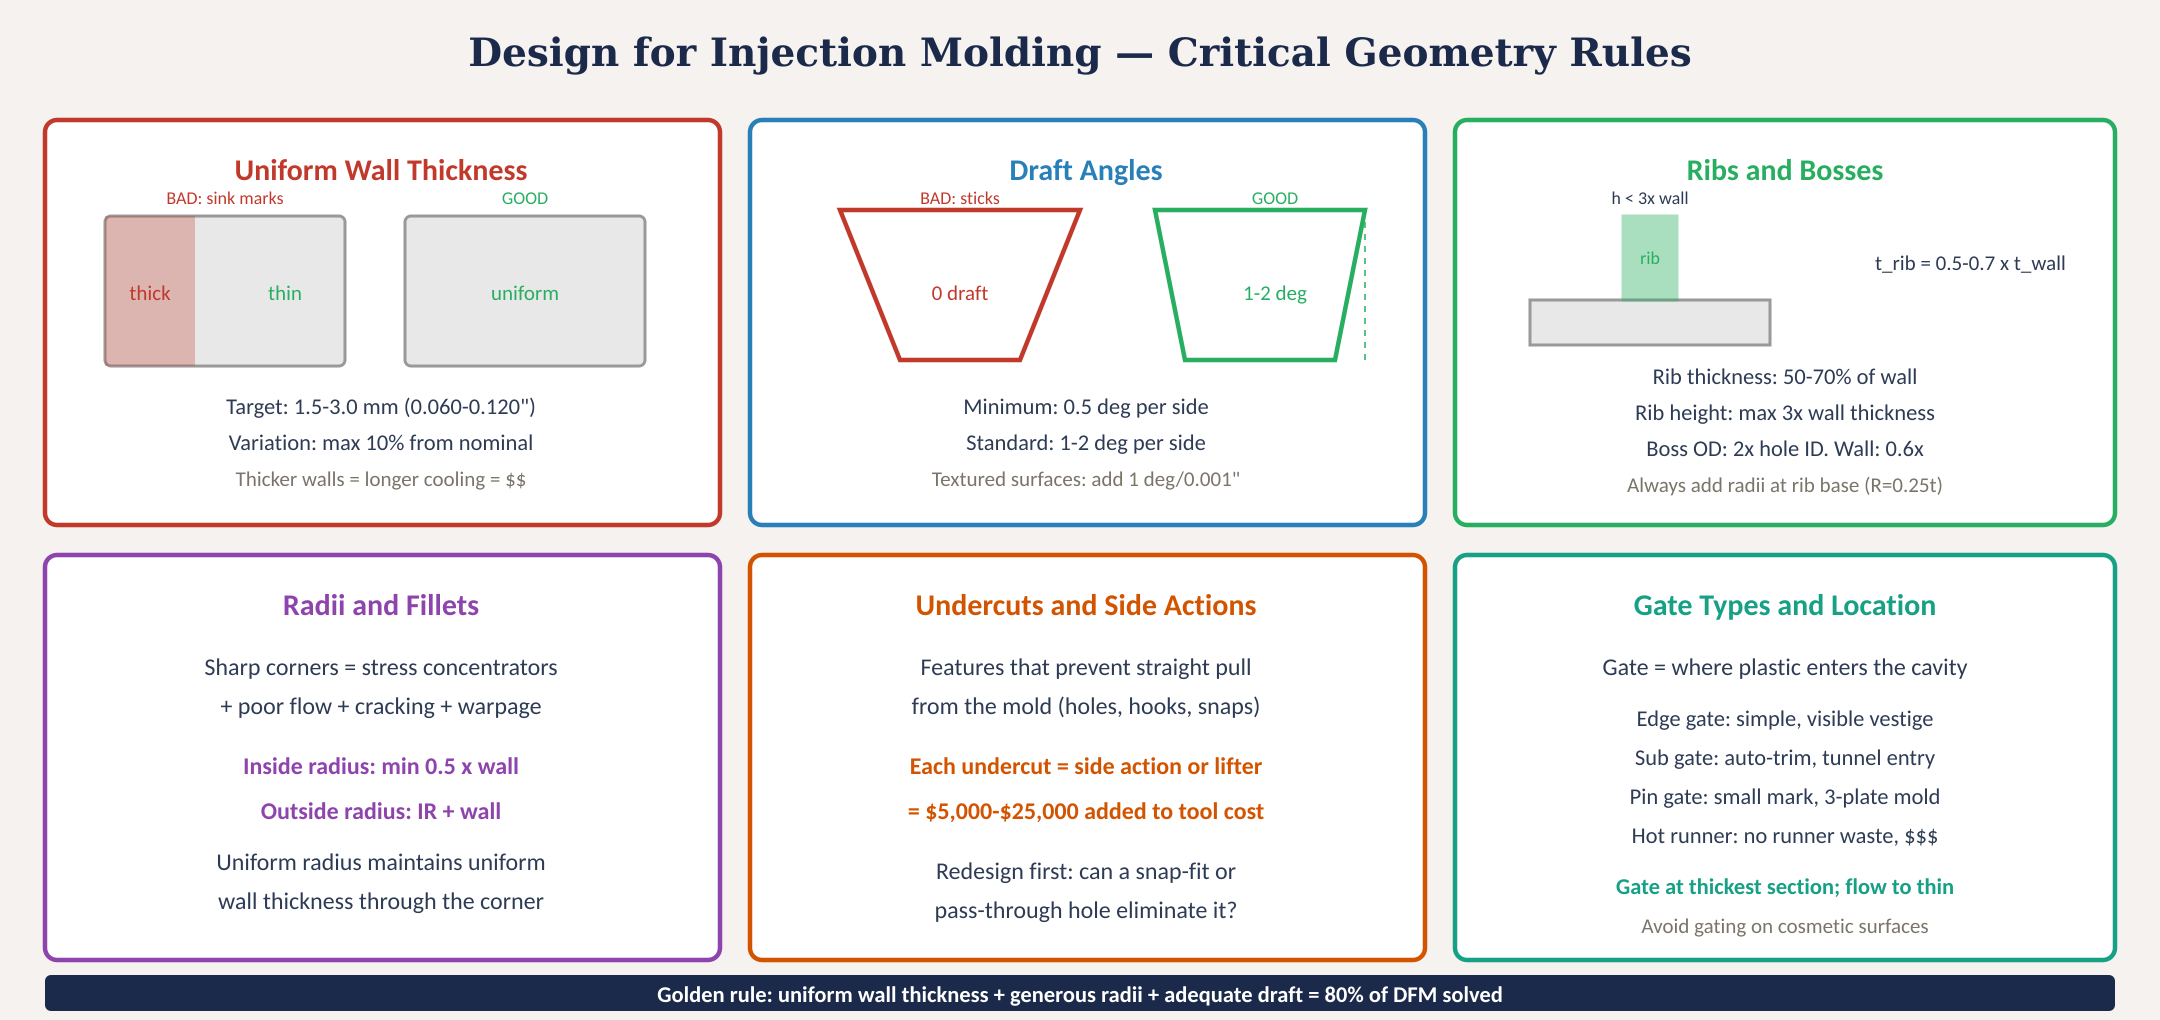
\includegraphics[width=\textwidth]{master_figs/fig_dfm_rules.png}
\caption{Six critical DFM geometry rules: wall thickness, draft angles, ribs/bosses, radii, undercuts, and gate location.}
\label{fig:dfm}
\end{figure}

\subsection{Rule 1: Uniform Wall Thickness}

The single most important design parameter. Wall thickness drives cycle time (cooling $\propto t^2$), material usage, shrinkage uniformity, and defect susceptibility.

\textbf{Recommended ranges}: ABS: 1.5--3.5\,mm. PC: 1.5--3.5\,mm. PP: 0.8--3.0\,mm. Nylon: 1.0--3.0\,mm. POM: 1.0--3.0\,mm.

\textbf{Uniformity}: Variation $<$10\% of nominal. Where transitions are unavoidable, use gradual tapers at a 3:1 length-to-thickness-change ratio. Abrupt steps cause differential shrinkage, sink marks, and stress concentrations.

\textbf{Coring out}: Replace solid thick sections with thin uniform shells reinforced by ribs. A ribbed 2\,mm wall is stiffer than a solid 4\,mm wall, cools in one-quarter the time, and uses half the material.

\subsection{Rule 2: Draft Angles}

Draft is the slight taper on walls parallel to the mold opening direction that allows the part to release.

\begin{itemize}[nosep,leftmargin=1.5em]
  \item Minimum: \ang{0.5} per side (tight tolerance applications).
  \item Standard: \ang{1}--\ang{2} per side (recommended).
  \item Textured surfaces: add \ang{1} per 0.001\,in (0.025\,mm) of texture depth.
  \item Core side often needs more draft than cavity side (part shrinks onto core).
\end{itemize}

\begin{warningbox}[Zero-Draft = Stuck Parts]
Zero-draft vertical walls are the \#1 student DFM error. Without draft, the part grips the core, ejector pins push through the wall, and the mold wears rapidly. Apply draft to \emph{all} surfaces parallel to the pull direction; including internal ribs, bosses, and walls.
\end{warningbox}

\subsection{Rule 3: Ribs and Bosses}

Ribs add stiffness without mass; bosses provide screw/insert mounting points.

\subsubsection{Rib Proportions}
\begin{itemize}[nosep,leftmargin=1.5em]
  \item Thickness: 50--70\% of adjoining wall (thicker $\to$ sink marks on opposite surface).
  \item Height: max $3\times$ wall thickness (taller $\to$ fill and ejection problems).
  \item Draft: min \ang{0.5} per side (\ang{1} preferred).
  \item Spacing: min $2\times$ wall thickness between ribs.
  \item Base radius: 0.25--0.5 $\times$ wall thickness.
  \item Multiple thin ribs outperform one thick rib.
\end{itemize}

\subsubsection{Boss Proportions}
\begin{itemize}[nosep,leftmargin=1.5em]
  \item OD: 2.0--2.5 $\times$ screw/insert hole ID.
  \item Wall: 0.6 $\times$ nominal wall thickness.
  \item Freestanding bosses: connect to nearest wall with a rib.
  \item Height: max 2.5 $\times$ OD.
  \item For heat-set brass inserts: hole ID per insert manufacturer specification.
\end{itemize}

\subsection{Rule 4: Radii and Fillets}

Sharp inside corners create stress concentrations (up to $3\times$ at zero radius), impede melt flow, and cause sink marks.

\begin{itemize}[nosep,leftmargin=1.5em]
  \item Inside radius: min $0.5\times$ wall (1$\times$ preferred).
  \item Outside radius: inside radius $+$ wall thickness.
  \item This maintains uniform wall thickness through the corner.
  \item Apply radii to \emph{every} inside corner without exception.
\end{itemize}

\subsection{Rule 5: Undercuts}

Any feature preventing straight-pull mold separation; side holes, snap hooks, internal threads, louvers. Each undercut requires a side action (cam, lifter, or collapsing core), adding \$5,000--\$25,000 to tooling cost.

\textbf{Always redesign first}: Can a pass-through hole replace a blind side hole? Can a snap-fit be oriented along the pull direction? Can an internal thread become a heat-set insert installed after molding?

\subsection{Rule 6: Gate Location}

The gate is where plastic enters the cavity.

\begin{itemize}[nosep,leftmargin=1.5em]
  \item \textbf{Place at the thickest section} so melt flows from thick to thin (ensures adequate packing).
  \item \textbf{Never gate on a cosmetic surface}; the gate vestige is always visible.
  \item Gate types: edge gate (simple, visible mark), sub gate (auto-trimmed), pin gate (small mark, 3-plate mold), hot runner (no runner waste, highest tooling cost).
  \item Flow simulation (Moldflow) predicts fill pattern and weld line locations.
\end{itemize}


% ══════════════════════════════════════════════════════════════════════
\section{Common Defects}
\label{sec:defects}
% ══════════════════════════════════════════════════════════════════════

Every defect has a root cause in part geometry, material, or process. Good design eliminates most defects before the mold is ever cut.

\begin{figure}[htbp]
\centering
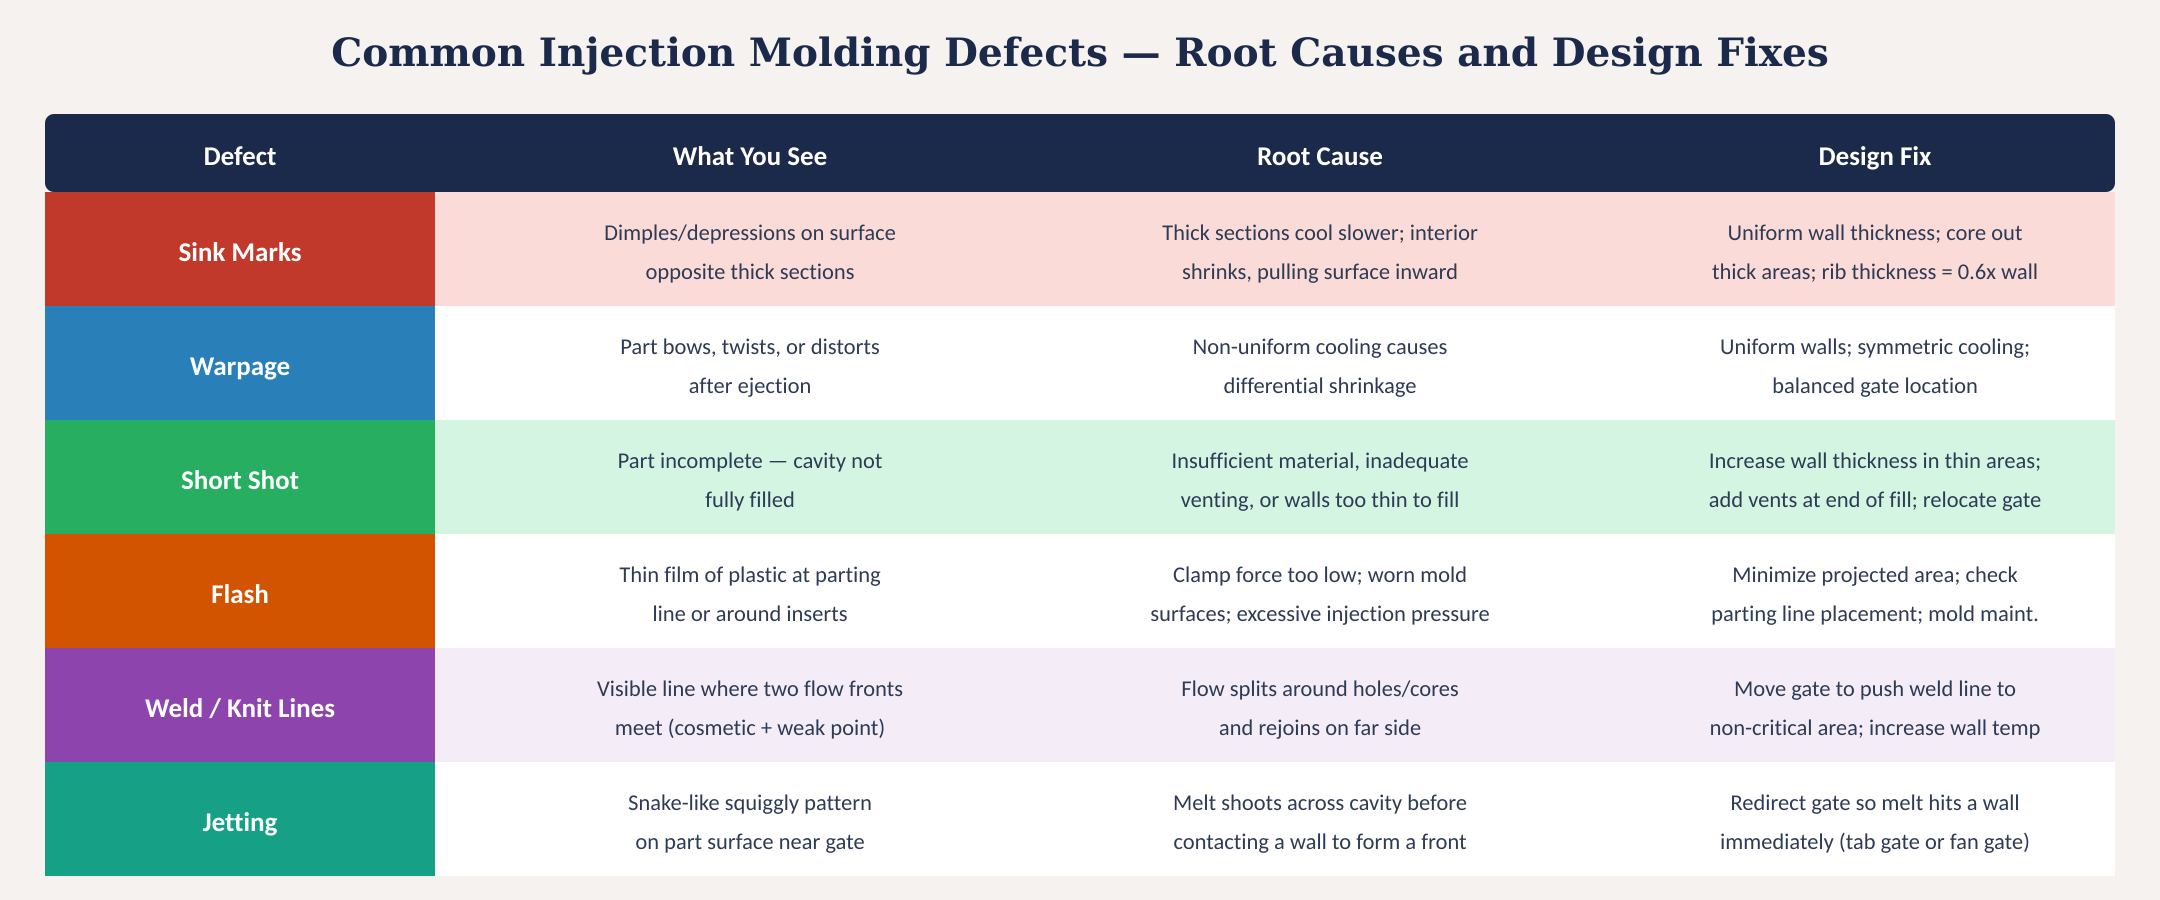
\includegraphics[width=\textwidth]{master_figs/fig_defects.png}
\caption{Six common injection molding defects with visual description, root cause, and design fix.}
\label{fig:defects}
\end{figure}

\begin{table}[htbp]
\centering\small
\begin{tabularx}{\textwidth}{l l X X}
  \toprule
  \textbf{Defect} & \textbf{What You See} & \textbf{Root Cause} & \textbf{Design Fix} \\
  \midrule
  Sink marks & Dimples opposite thick sections & Thick areas cool slowly, interior shrinks & Uniform walls; core out; rib = 0.6$\times$ wall \\
  Warpage & Part bows/twists after ejection & Non-uniform cooling $\to$ differential shrinkage & Uniform walls; symmetric cooling; balanced gate \\
  Short shot & Incomplete part & Inadequate venting, thin walls, low pressure & Vent at end of fill; increase thin walls \\
  Flash & Thin film at parting line & Low clamp force, worn mold, high pressure & Minimize projected area; mold maintenance \\
  Weld lines & Visible line where fronts meet & Flow splits around holes/cores & Relocate gate; increase melt temperature \\
  Jetting & Squiggly pattern near gate & Melt shoots across cavity before wall contact & Redirect gate so melt hits a wall immediately \\
  \bottomrule
\end{tabularx}
\caption{Common defects, root causes, and design fixes.}
\end{table}

\begin{tipbox}[Weld Line Strength]
Weld lines retain only 50--90\% of base material strength. If a weld line falls on a load-bearing feature, relocate the gate or add ribs to reinforce. Flow simulation is the primary tool for predicting and relocating weld lines before cutting the mold.
\end{tipbox}


% ══════════════════════════════════════════════════════════════════════

\subsection{Worked DFM Example: Sensor Enclosure}
\textbf{Requirements}: outdoor IP65 enclosure for GreenShield controller, ABS material, holds PCB (60$\times$40\,mm) and two cable glands.

\textbf{Design decisions}:
\begin{itemize}[nosep,leftmargin=1.5em]
\item \textbf{Wall thickness}: 2.0\,mm uniform (ABS range: 1.5--3.5\,mm). Adequate for IP65 with gasket groove.
\item \textbf{Draft}: \ang{2} on all external walls. C-1 matte finish; no additional texture draft needed.
\item \textbf{Ribs}: four internal ribs at 1.2\,mm thick ($0.6 \times 2.0$), 6.0\,mm tall ($3 \times 2.0$), connecting the PCB mounting bosses to the walls. Base radius 0.5\,mm.
\item \textbf{Bosses}: four PCB mounting bosses, OD = 6.0\,mm ($2.5 \times 2.4$\,mm screw), wall = 1.2\,mm, height = 10\,mm. Each connected to nearest wall by a rib.
\item \textbf{Radii}: all inside corners 1.0\,mm ($0.5 \times 2.0$\,mm wall). Outside corners 3.0\,mm (inside + wall).
\item \textbf{Sealing}: 1.5\,mm wide $\times$ 1.0\,mm deep O-ring groove around the lid perimeter. Silicone O-ring (cord dia.\ 1.5\,mm, compressed to 75\% = 1.0\,mm groove depth).
\item \textbf{Gate}: edge gate on the bottom face (non-cosmetic), at the thickest section near a rib intersection.
\item \textbf{Parting line}: at the lid/base junction (natural split).
\end{itemize}

\section{Tooling and Economics}
\label{sec:tooling}
% ══════════════════════════════════════════════════════════════════════

\begin{figure}[htbp]
\centering
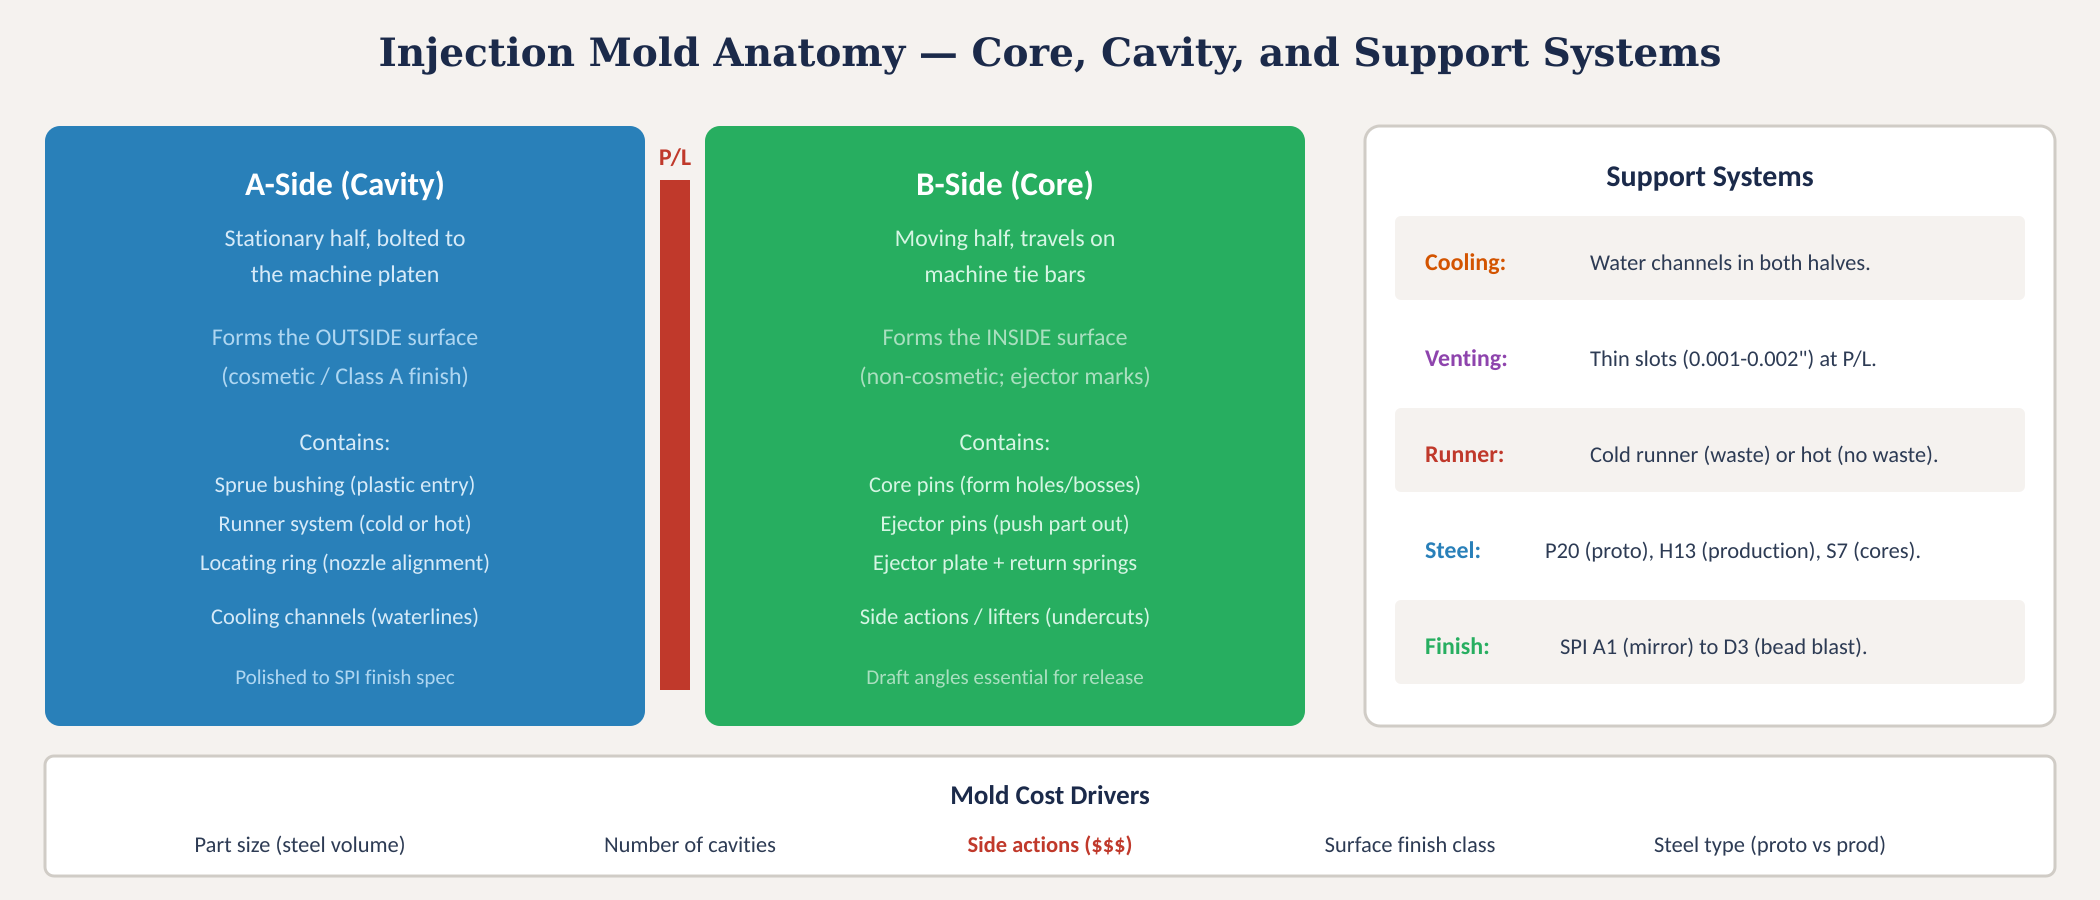
\includegraphics[width=\textwidth]{master_figs/fig_mold_anatomy.png}
\caption{Mold anatomy: A-side (cavity), B-side (core), parting line, support systems, and cost drivers.}
\label{fig:mold}
\end{figure}

\subsection{Mold Construction}

The \textbf{A-side} (cavity) forms the cosmetic outside surface. It contains the sprue bushing, runner system, and locating ring. Surfaces are polished to SPI specifications (A-1 mirror to D-3 bead blast). The \textbf{B-side} (core) forms the inside surface and contains core pins, ejector pins, ejector plates, and side actions. The parting line between the halves leaves a witness mark on the part.

\textbf{Support systems}: cooling channels (water lines in both halves; conformal cooling can reduce cycle time 20--40\%), venting (thin slots 0.001--0.002\,in at parting line), runner system (cold runner produces waste; hot runner eliminates waste but costs more), and ejection system (pins, sleeves, blades, stripper plates).

\subsection{Mold Classifications (SPI)}

\begin{table}[htbp]
\centering\small
\begin{tabularx}{\textwidth}{l l l l X}
  \toprule
  \textbf{Class} & \textbf{Steel} & \textbf{Life (cycles)} & \textbf{Cost Range} & \textbf{Use} \\
  \midrule
  105 (Prototype) & Aluminum / soft steel & $<$500 & \$5K--\$15K & Design validation, pilot runs \\
  104 (Low Prod.) & P20 pre-hardened & $<$100K & \$15K--\$50K & Low volume, bridge tooling \\
  103 (Med. Prod.) & H13 hardened & $<$500K & \$30K--\$80K & Medium-volume production \\
  101 (High Prod.) & Premium hardened & 1M+ & \$50K--\$200K+ & High-volume, long-life production \\
  \bottomrule
\end{tabularx}
\caption{SPI mold classifications.}
\end{table}

\subsection{Part Cost Economics}

\begin{equation}
  C_{\text{part}} = C_{\text{material}} + C_{\text{cycle}} + C_{\text{tooling,amortized}}
\end{equation}

where $C_{\text{material}} = \text{weight} \times \text{resin cost}$, $C_{\text{cycle}} = \text{cycle time} \times \text{machine rate} / 3600$, and $C_{\text{tooling}} = \text{mold cost} / \text{expected lifetime parts}$.

\textbf{Example} (small ABS enclosure, 30\,g): Material: \$0.06. Cycle (25\,s at \$60/hr): \$0.42. Tooling (\$25K amortized over 50K parts): \$0.50. \textbf{Total: \$0.98/part}. At 500K parts, tooling drops to \$0.05/part, total \$0.53/part.

Injection molding breaks even versus 3D printing at approximately 100--500 parts depending on part size and complexity. Below that, 3D printing is cheaper; above it, injection molding wins dramatically.




\section{Warpage}
Warpage is dimensional distortion that occurs after ejection. It is caused by differential shrinkage: when different regions of the part cool at different rates or have different molecular orientations, they shrink by different amounts, creating internal stresses that bow or twist the part.

\subsection{Causes of Warpage}
\textbf{Differential cooling}: one side of the wall cools faster (e.g., mold steel temperature differs between A-side and B-side). The slow-cooling side shrinks more after ejection, bowing the part toward it. \textbf{Fiber orientation}: glass-filled materials shrink less in the flow direction than across it; 0.3\% vs.\ 0.8\% creates a 0.5\% differential. \textbf{Gate location}: determines flow pattern and therefore orientation pattern. A poorly placed gate creates asymmetric flow that maximizes differential shrinkage.

\subsection{Designing to Minimize Warpage}
\begin{itemize}[nosep,leftmargin=1.5em]
\item Maintain uniform wall thickness ($\pm$10\%).
\item Equalize cooling on both sides (symmetric cooling channels).
\item Use gating that produces symmetric flow.
\item For glass-filled materials, gate at center to produce radial (symmetric) fiber orientation.
\item Add ribs to resist bowing (ribs on the concave side of expected warp).
\end{itemize}

\section{Surface Finish}
\subsection{SPI (PIA) Finish Standards}
Surface finish is specified using SPI (Society of the Plastics Industry, now PIA) standards:

\begin{table}[htbp]\centering\small
\begin{tabularx}{\textwidth}{l l l X}
\toprule
\textbf{Grade} & \textbf{Finish} & \textbf{Ra ($\mu$m)} & \textbf{Method and Application} \\
\midrule
A-1 & Mirror & 0.012 & Diamond buff. Optical lenses, light pipes. \\
A-2 & High gloss & 0.025 & Diamond buff. Cosmetic consumer products. \\
B-1 & Semi-gloss & 0.05 & 600 grit paper. General cosmetic surfaces. \\
C-1 & Matte & 0.35 & 600 stone. Hides sink marks, fingerprints. \\
D-1 & Textured & 1.0 & Dry blast. Grips, non-slip, industrial. \\
D-3 & Rough texture & 3.2 & Coarse blast. Heavily textured panels. \\
\bottomrule
\end{tabularx}
\caption{SPI/PIA mold surface finish standards.}
\end{table}

Higher polish = higher mold cost. C-1 matte is the sweet spot for most student and industrial enclosures; hides minor defects while maintaining a professional appearance.

\subsection{Textured Surfaces and Draft}
Texture creates an effective undercut. Add \ang{1} of additional draft per 0.001\,in (0.025\,mm) of texture depth. A D-1 texture (1.0\,$\mu$m Ra, $\$\sim\$$0.001\,in depth) requires \ang{1} extra draft beyond the baseline. Failing to add texture draft causes drag marks during ejection.

\section{Insert Molding and Overmolding}
\subsection{Insert Molding}
A pre-formed component (metal insert, PCB, bushing) is placed in the mold before injection. Plastic flows around and bonds to the insert. Use when you need: threaded metal inserts (stronger than threading into plastic), electrical contacts molded into a housing, or reinforcing metal structures embedded in plastic.

Design rules: provide $\geq$1.5\,mm of plastic around the insert, add knurling or grooves for mechanical interlock, preheat metal inserts to reduce thermal shock stress, and ensure the insert is fixtured precisely.

\subsection{Overmolding}
A second material is molded over a previously molded substrate. Two-shot or two-step process. Common application: soft TPE grip over rigid ABS body (power tools, toothbrushes, medical devices). The two materials must be chemically compatible for adhesion. Common pairs: ABS/TPE, PC/TPE, nylon/TPE.

\section{Living Hinges and Snap-Fit Clips}
\subsection{Living Hinges}
A living hinge is a thin, flexible web of plastic that connects two rigid sections, allowing them to flex repeatedly without breaking. \textbf{Polypropylene (PP)} is the only commonly injection-molded material suitable for living hinges; its molecular structure allows millions of flex cycles without fatigue. Design rules: hinge thickness 0.25--0.50\,mm, web length 1.0--1.5\,mm, flex immediately after molding (orients molecules across the hinge, increasing life by $10\times$), and gate so flow is perpendicular to the hinge line.

\begin{tipbox}[Material Matters]
ABS, PC, and nylon all crack at a living hinge within a few cycles. \textbf{Only PP} (and some PE grades) can survive millions of flexes. If your design needs a living hinge, the part must be PP; no exceptions.
\end{tipbox}

\subsection{Snap-Fit Clips}
Cantilever snaps are the most common: a beam deflects during assembly, then locks behind a lip. Design for the allowable strain of your material: 2\% for ABS, 4\% for PP, 1.5\% for PC. Maximum deflection: $y = \epsilon L^2 / (1.5t)$ where $\epsilon$ = allowable strain, $L$ = beam length, $t$ = beam thickness. Include a lead-in angle (30--45$^{\circ}$) for easy assembly and a steeper retaining angle (80--90$^{\circ}$) for secure locking. Snap-fits eliminate screw hardware; a significant DFA (Design for Assembly) advantage.

% ══════════════════════════════════════════════════════════════════════
\section{Artifact Handoff: What This Chapter Supports}
\begin{table}[htbp]\centering\small
\begin{tabularx}{\textwidth}{l X l}
\toprule
\textbf{Artifact} & \textbf{Description} & \textbf{Forward Reference} \\
\midrule
DFM Review & Checklist verification for each molded part & CDR deliverable \\
Material Selection & Resin choice with shrinkage and property data & BOM, tolerance analysis \\
Tooling Estimate & Mold class, cost, and timeline & Budget, schedule \\
\bottomrule
\end{tabularx}
\end{table}

\section{DFM Checklist}
\label{sec:checklist_b}
% ══════════════════════════════════════════════════════════════════════

Review every item before sending your CAD model to a molder.

\begin{enumerate}[leftmargin=1.5em]
  \item Wall thickness uniform ($\pm$10\%)? Within recommended range for material?
  \item Draft angles applied to ALL surfaces parallel to pull direction? Texture draft added?
  \item Ribs at 50--70\% of wall? Height $\leq 3\times$ wall? Base radii present?
  \item Bosses at $2\times$ hole ID? Connected to walls with ribs? Boss wall $\leq 0.6\times$ nominal?
  \item All inside corners radiused (min $0.5\times$ wall)? Outside radius = inside + wall?
  \item Undercuts identified? Side actions justified or redesigned out?
  \item Gate location at thickest section? Not on cosmetic surface?
  \item Parting line location acceptable on finished part?
  \item Ejector pin locations on non-cosmetic surfaces? Adequate draft for release?
  \item Shrinkage accounted for in critical dimensions? Tolerances achievable ($\pm$0.005\,in typical)?
  \item Material selected? Properties verified against operating conditions?
  \item Moldflow or fill analysis run? Weld lines and air traps identified?
\end{enumerate}

\begin{warningbox}[Fix Problems in CAD, Not in Steel]
Fixing a design problem in CAD takes minutes. Finding the same problem after the mold is cut costs \$5,000--\$20,000 in mold modifications and 2--4 weeks of delay. Run this checklist at your CDR before committing to tooling.
\end{warningbox}

\begin{keyconceptbox}[Requirements Mapping: From DFM Rules to Shall-Statements]
Injection molding constraints generate system requirements:
\begin{itemize}[nosep,leftmargin=1.5em]
\item ``Part must survive 1\,m drop onto concrete'' $\to$ MAT-REQ: Material shall have Izod impact $\geq$200\,J/m (ABS or PC/ABS).
\item ``Outdoor enclosure, 5+ year UV exposure'' $\to$ MAT-REQ: Material shall be UV-stabilized or painted.
\item ``Volume 50K units/year'' $\to$ TOOL-REQ: Mold shall be SPI Class~104 (P20 steel, $\leq$100K cycle life).
\item ``Assembly time $<$30\,s'' $\to$ DFA-REQ: Enclosure shall use snap-fit closure (no fasteners). Cantilever strain $\leq$2\% for ABS.
\end{itemize}
\end{keyconceptbox}


% ══════════════════════════════════════════════════════════════════════
\section{Practice Questions}
\label{sec:practice_b}
% ══════════════════════════════════════════════════════════════════════

\subsection{Conceptual Questions}

\begin{enumerate}[leftmargin=1.5em]
  \item Why does cooling time scale with the \emph{square} of wall thickness rather than linearly? How does this affect part cost?

  \item A part has a 4\,mm thick boss connected to a 2\,mm wall. Predict the defect you will see on the surface opposite the boss. What is the design fix?

  \item Explain why a part shrinks onto the core side of the mold during cooling. How does this affect draft angle requirements for the core versus cavity sides?

  \item Your part has a snap hook that creates an undercut on one side. The molder quotes \$18,000 for the side action. Propose two redesign alternatives that might eliminate the side action.

  \item Compare ABS and polypropylene for a consumer electronics enclosure that must accept paint and withstand a 1-meter drop test. Which do you recommend and why?

  \item Why must the gate be placed at the thickest section? What happens if you gate at a thin section instead?

  \item A textured surface (SPI D-2, depth $\approx$ 0.002\,in) on a 3-inch-deep wall currently has \ang{1} of draft. Is this sufficient? If not, what is the correct draft angle?
\end{enumerate}

\subsection{Application / Scenario Questions}

\begin{enumerate}[resume,leftmargin=1.5em]
  \item You are designing a two-piece snap-fit enclosure for an IoT sensor that will be installed outdoors. The enclosure must be IP65, withstand $-20$ to $+60$\,\degC, resist UV for 5+ years, and cost under \$3/part at 10,000 units. Select the material, specify wall thickness, describe the snap-fit design, and estimate whether injection molding is economically justified.

  \item Your teammate's CAD model for a motor mount bracket has: 5\,mm walls, zero draft on all vertical surfaces, sharp inside corners, and a boss with OD = 1.5$\times$ hole ID. List every DFM violation, predict the defects that will result from each, and specify the corrected dimensions.

  \item \textbf{Cost analysis}: A part weighs 45\,g in PC/ABS (\$0.003/g). Cycle time is 30\,seconds on a machine at \$75/hr. The mold costs \$35,000. Calculate the total part cost at 5,000, 50,000, and 500,000 units. At what volume does injection molding become cheaper than SLA 3D printing at \$8.50/part?
\end{enumerate}

\subsection{Answers}

\begin{enumerate}[leftmargin=1.5em]
  \item Cooling is a transient heat-conduction problem governed by the Fourier equation. The characteristic time for heat to diffuse through a slab of thickness $t$ scales as $t^2 / \alpha$ where $\alpha$ is thermal diffusivity. Doubling wall thickness from 2\,mm to 4\,mm quadruples cooling time; potentially adding 20--40 seconds per cycle. At a machine rate of \$60/hr, each additional second costs approximately \$0.017/part. Over 100,000 parts, a 20-second cycle-time penalty costs \$17,000.

  \item A sink mark (dimple/depression) on the surface opposite the boss. The 4\,mm boss is twice the 2\,mm wall, creating a thick section that cools more slowly. The interior shrinks and pulls the surface inward. Fix: reduce boss wall to $0.6 \times 2 = 1.2$\,mm (OD = hole ID + 2$\times$1.2\,mm). Connect the boss to the nearest wall with a thin rib.

  \item As plastic cools it contracts volumetrically. The cavity half forms the outside surface, and the part shrinks \emph{away} from it, naturally releasing. The core half forms the inside surface, and the part shrinks \emph{onto} it, gripping tighter as it cools. This means the core side typically needs more draft (\ang{1.5}--\ang{2}) than the cavity side (\ang{0.5}--\ang{1}) to overcome the shrink-grip.

  \item (a) Reorient the snap hook to flex along the mold-open direction; if the hook can deflect during ejection, no side action is needed (the hook ``snaps'' past the mold surface). (b) Replace the snap hook with a separate clip that installs post-molding via a push-fit or ultrasonic weld, eliminating the undercut entirely.

  \item ABS. Both have adequate impact strength, but ABS accepts paint directly (smooth surface, good adhesion) while PP requires flame treatment or specialty primers due to its low surface energy. ABS also has a higher HDT ($\$\sim\$$95\,$^{\circ}$C versus $\$\sim\$$60\,$^{\circ}$C for unfilled PP), providing more thermal margin. ABS shrinkage (0.5--0.7\%) is lower and more predictable than PP (1.0--2.5\%), enabling tighter dimensional control for snap-fits and mating features.

  \item Gating at the thickest section ensures that the section that shrinks the most remains connected to the runner for packing pressure the longest. If you gate at a thin section, the thin area freezes first and seals off (``gates off''), cutting the thick section off from packing pressure. The result is severe sink marks and voids in the thick section because the material cannot be replenished as it shrinks.

  \item No. The texture-depth rule requires adding \ang{1} per 0.001\,in of depth. At 0.002\,in depth, add \ang{2} beyond the standard \ang{1} for a total of \ang{3} per side. Without adequate draft, the textured surface acts like sandpaper during ejection, leaving drag marks that ruin the finish and gouge the mold steel.

  \item Material: ASA (acrylic-styrene-acrylonitrile), UV-stable variant of ABS, good impact from $-20$ to $+80$\,\degC, IP65-rated with proper gasket design, paintable if needed. Wall thickness: 2.0\,mm nominal (meets structural requirements, enables IP65 with perimeter gasket groove). Snap-fit: cantilever snaps along the mold-open axis (no side action), 2\% max strain for ASA, designed with \ang{1.5} draft. Economics: at 10,000 units with a Class~104 mold (\$25K), tooling amortization is \$2.50/part. Material (20\,g $\times$ \$0.003): \$0.06. Cycle (20\,s at \$60/hr): \$0.33. Total: $\$\sim\$$\$2.89/part, under the \$3 target. Injection molding is justified.

  \item Violations and fixes: (a) 5\,mm walls are too thick for any common plastic; excessive cooling time, sink marks, voids. Fix: core out to 2\,mm uniform walls, add ribs for stiffness. (b) Zero draft on all vertical surfaces; parts will stick, ejector damage, mold wear. Fix: add minimum \ang{1} per side to all surfaces parallel to pull. (c) Sharp inside corners; stress concentrations ($3\times$ multiplier), impeded flow. Fix: add $R = 0.5 \times 2 = 1$\,mm fillet to all inside corners; outside radius = $1 + 2 = 3$\,mm. (d) Boss OD at $1.5\times$ hole ID is too thin-walled, creating a thick ring that sinks. Fix: increase OD to $2.0\times$ hole ID. Predicted defects: sink marks everywhere (thick walls + oversized boss), warpage (non-uniform cooling from variable thickness), ejection damage (no draft), cracking at corners under load (no radii).

  \item Material: $45 \times 0.003 = \$0.135$/part. Cycle: $30/3600 \times 75 = \$0.625$/part. These are constant.

  At 5,000 parts: tooling $= 35000/5000 = \$7.00$/part. Total: $\$7.76$/part.

  At 50,000 parts: tooling $= 35000/50000 = \$0.70$/part. Total: $\$1.46$/part.

  At 500,000 parts: tooling $= 35000/500000 = \$0.07$/part. Total: $\$0.83$/part.

  Break-even vs.\ SLA at \$8.50/part: solve $0.135 + 0.625 + 35000/n = 8.50$. $35000/n = 7.74$. $n = 4,522$ parts. Above $\$\sim\$$4,500 parts, injection molding is cheaper.
\end{enumerate}


% ══════════════════════════════════════════════════════════════════════




\subsection{Application / Scenario Questions}
\begin{enumerate}[leftmargin=1.5em, start=7]
\item You are designing an outdoor sensor enclosure in ABS. The enclosure must be IP65 (dust-tight, water-jet resistant). Specify: wall thickness, draft angles, sealing method, and surface finish. Justify each choice.
\item A client asks you to injection mold a part with a living hinge. They want to use ABS because it matches the rest of their product line. What do you tell them?
\item Your injection-molded part has sink marks opposite the boss locations. The bosses are 3.0\,mm wall in a part with 2.0\,mm nominal wall. What is wrong, and how do you fix it?
\end{enumerate}

\subsection{Answers to Application Questions}
\begin{enumerate}[leftmargin=1.5em, start=7]
\item Wall: 2.0\,mm nominal (meets structural, enables IP65 with perimeter gasket groove). Draft: \ang{2} standard on all external walls; add \ang{1} per 0.001\,in of texture depth if textured. Sealing: silicone O-ring in a groove on the lid mating surface (not adhesive or gasket tape). Surface: C-1 matte (hides minor defects, professional appearance, reduces mold cost vs.\ polish). Internal surfaces: D-1 textured (hides ejector pin marks).
\item ABS cannot survive living hinge cycles; it will crack within 1--5 flexes. Only PP (and some PE) can form living hinges that last millions of cycles. Options: (a) redesign the part in PP; (b) use a separate PP living hinge piece bonded/overmolded to the ABS body; (c) replace the living hinge with a mechanical hinge (pin + knuckle) that can be molded in ABS.
\item Boss wall = 3.0\,mm vs.\ 2.0\,mm nominal = 150\% of wall thickness. This thick section cools slowly, creating a void that pulls the surface inward (sink mark). Fix: reduce boss wall to $0.6 \times 2.0 = 1.2$\,mm (60\% of nominal). If the boss needs more material for screw engagement, connect it to the nearest wall with a rib (rib at 60\% wall = 1.2\,mm).
\end{enumerate}

\chapter{Printed Circuit Board Design Fundamentals}

\vspace{1em}




\section{PCB Structure and Materials}

A printed circuit board is a layered sandwich of insulating substrate (FR-4 fiberglass-epoxy) with patterned copper conductors. Copper traces, pads, and planes are created by chemically etching unwanted copper from a continuous sheet. A \textbf{solder mask} (the green coating) protects copper from oxidation and shorts. A \textbf{silkscreen} layer prints component outlines and reference designators.

\begin{figure}[htbp]\centering
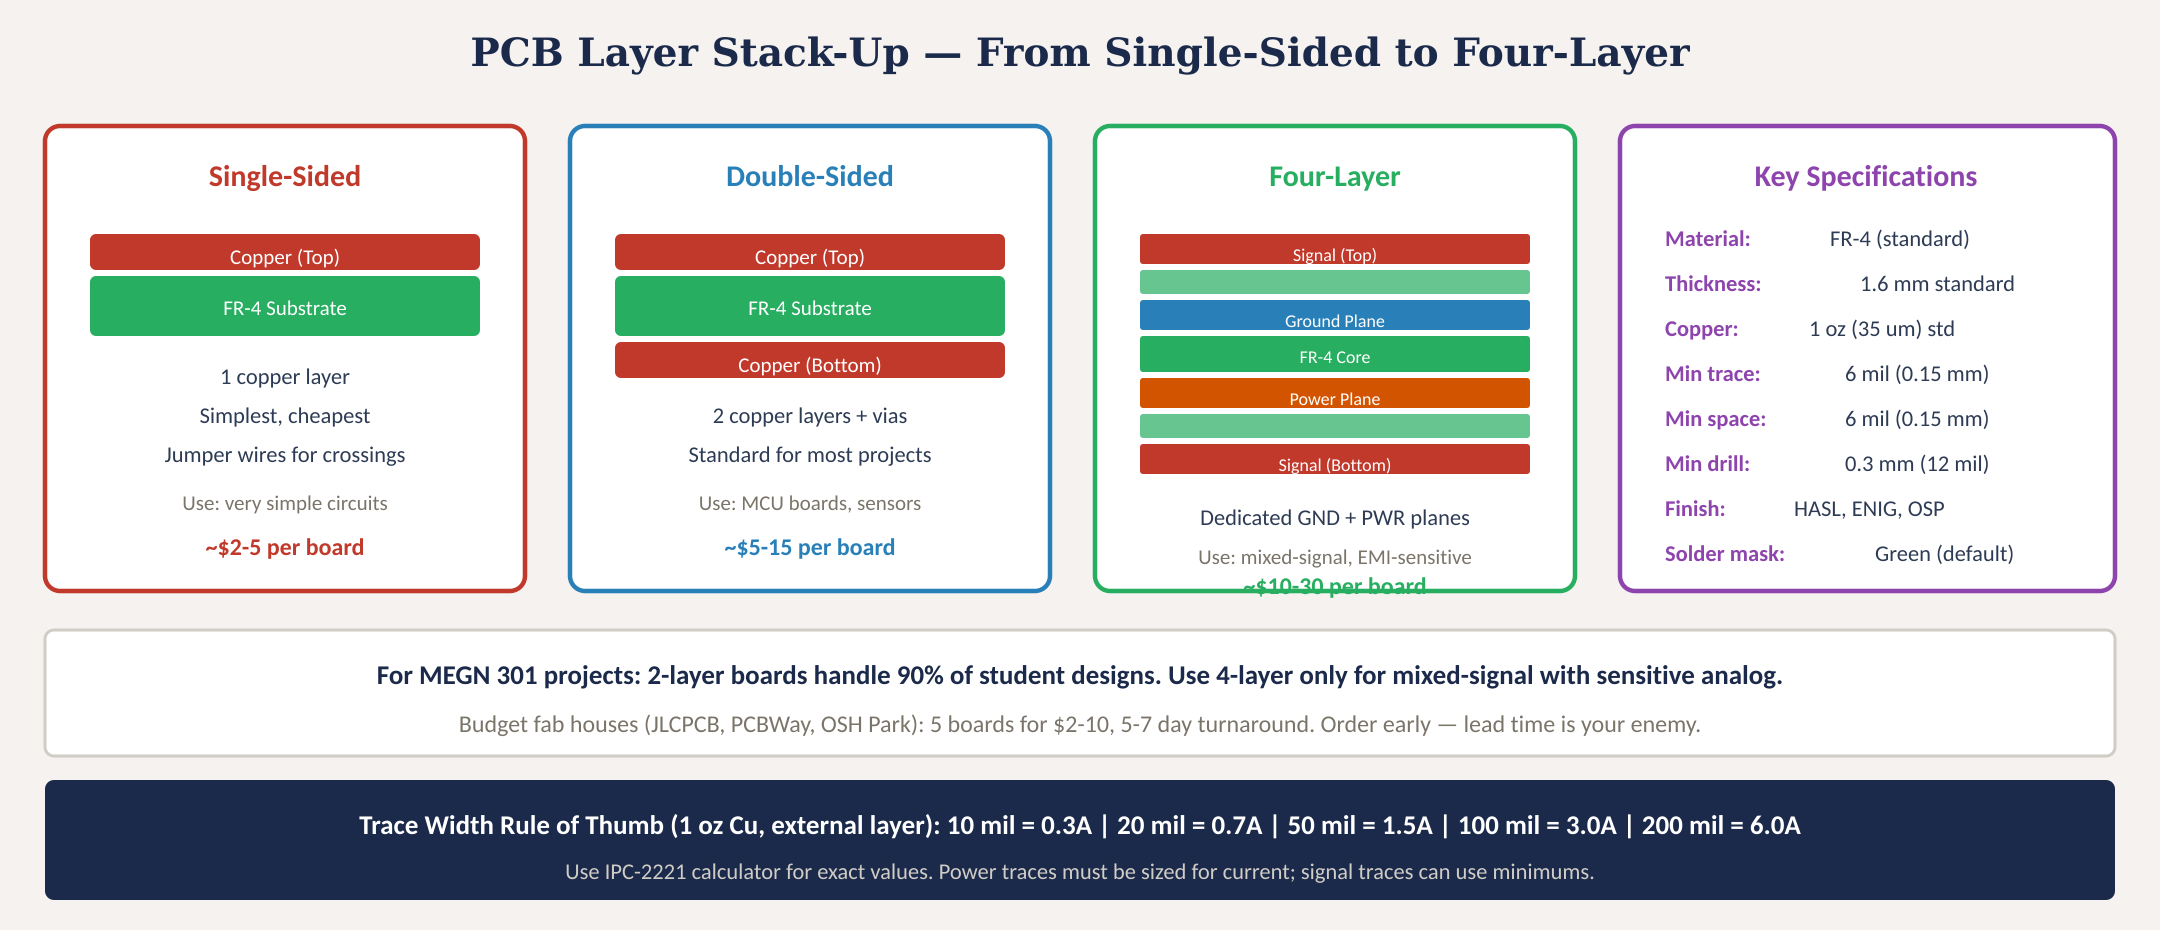
\includegraphics[width=\textwidth]{master_figs/fig_pcb_layer_stackup.png}
\caption{PCB layer stack-ups from single-sided to four-layer with key specifications and trace width current reference.}\label{fig:stack}
\end{figure}

\subsection{Layer Stack-Ups}
\textbf{Single-sided}: one copper layer. Simplest, cheapest (\$2--5). Jumper wires for crossings. Very simple circuits only. \textbf{Double-sided}: copper on both sides connected by vias (plated through-holes). Standard for 90\% of student projects (\$5--15). \textbf{Four-layer}: adds dedicated ground and power planes between signal layers. Use for mixed-signal or EMI-sensitive designs (\$10--30).

\subsection{Key Specifications}
FR-4 substrate, 1.6\,mm standard thickness, 1\,oz (35\,$\mu$m) copper, 6\,mil minimum trace/space, 0.3\,mm minimum drill. Surface finishes: HASL (cheapest, good for THT), ENIG (flat pads, good for SMD), OSP (organic, short shelf life).

\begin{warningbox}[Trace Width for Current]
A 10-mil trace on 1-oz external copper safely carries only 0.3\,A. Power traces must be sized for actual current: 10\,mil\,=\,0.3\,A, 20\,mil\,=\,0.7\,A, 50\,mil\,=\,1.5\,A, 100\,mil\,=\,3.0\,A, 200\,mil\,=\,6.0\,A. Use the IPC-2221 calculator for exact values. Signal traces can use minimums; power traces must be sized for current.
\end{warningbox}

\subsection{Component Packages}

\begin{figure}[htbp]\centering
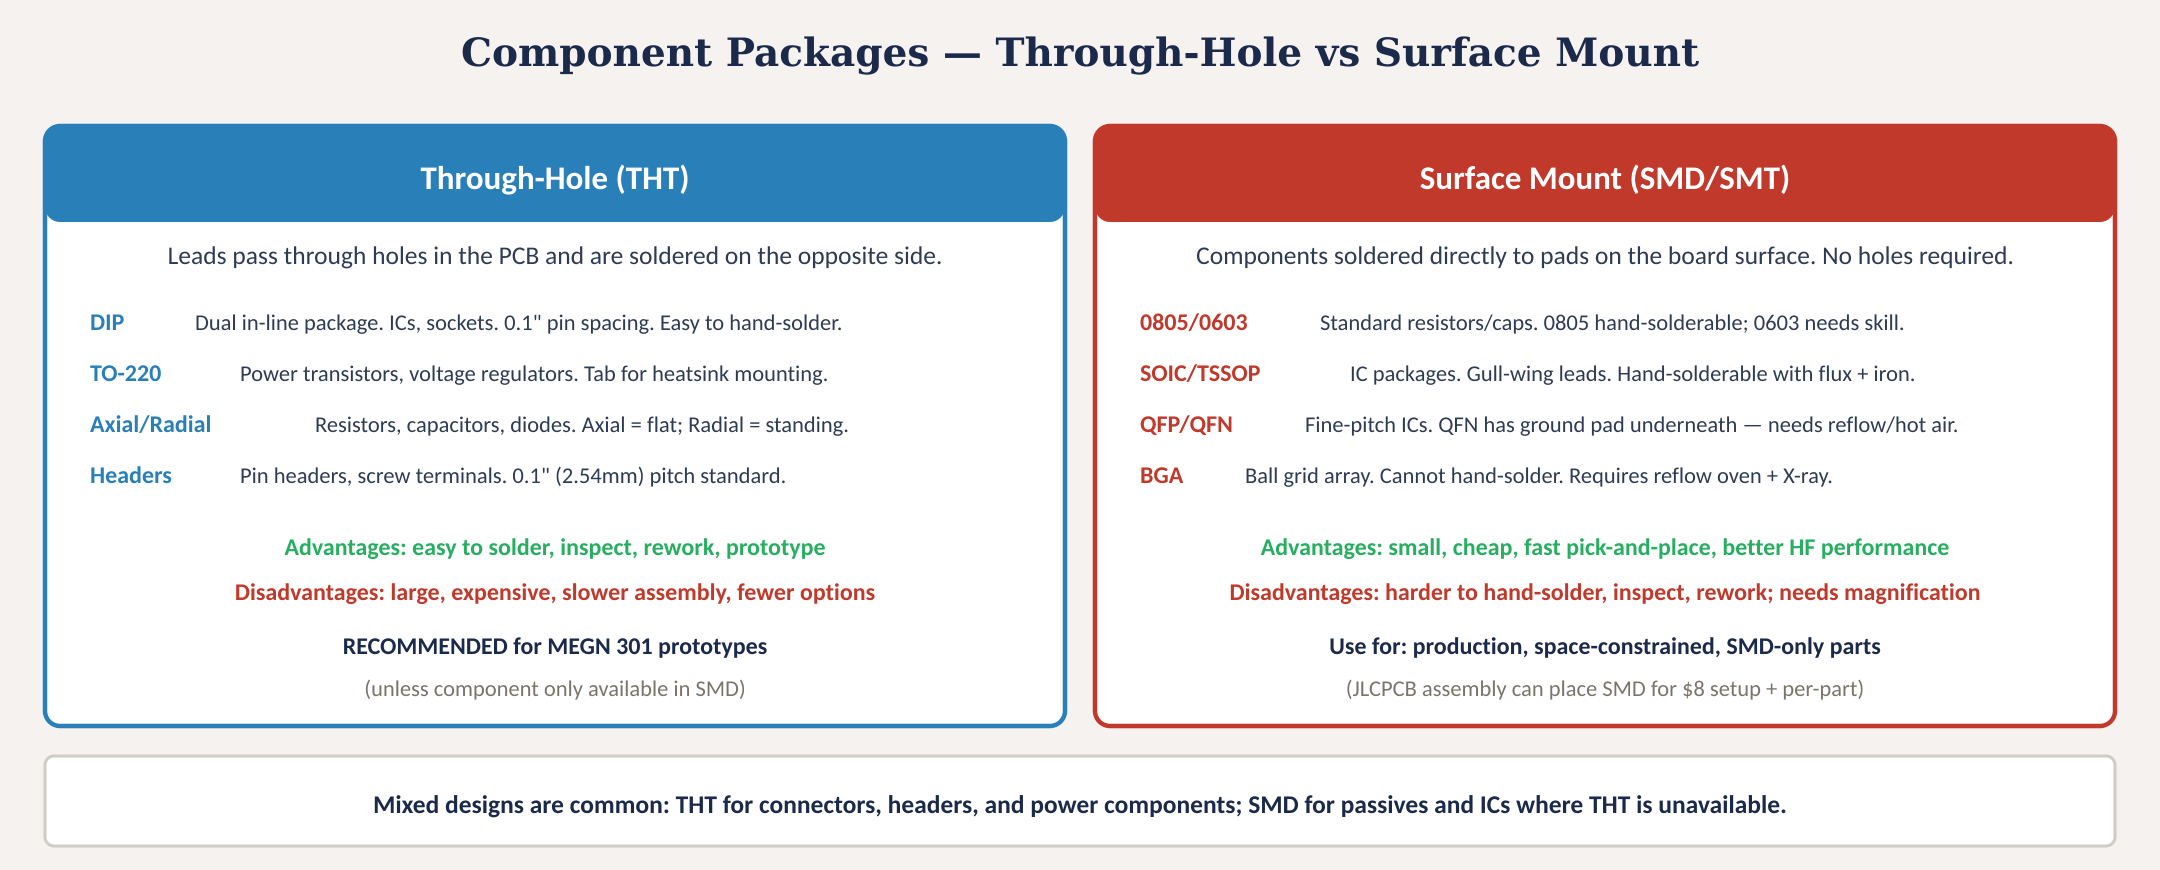
\includegraphics[width=\textwidth]{master_figs/fig_pcb_component_packages.png}
\caption{Through-hole vs surface-mount packages with common types and soldering guidance.}\label{fig:pkg}
\end{figure}

\textbf{Through-hole (THT)}: leads pass through holes. DIP, TO-220, axial/radial, pin headers. Easy to hand-solder, inspect, and rework. Recommended for MEGN 301 prototypes. \textbf{Surface-mount (SMD/SMT)}: soldered to pads on the board surface. 0805/0603 passives, SOIC/TSSOP ICs, QFP/QFN fine-pitch. Smaller, cheaper, but harder to hand-solder. Use SMD only when THT is unavailable or space is critical. Mixed designs are common.

\section{Design Workflow}

\begin{figure}[htbp]\centering
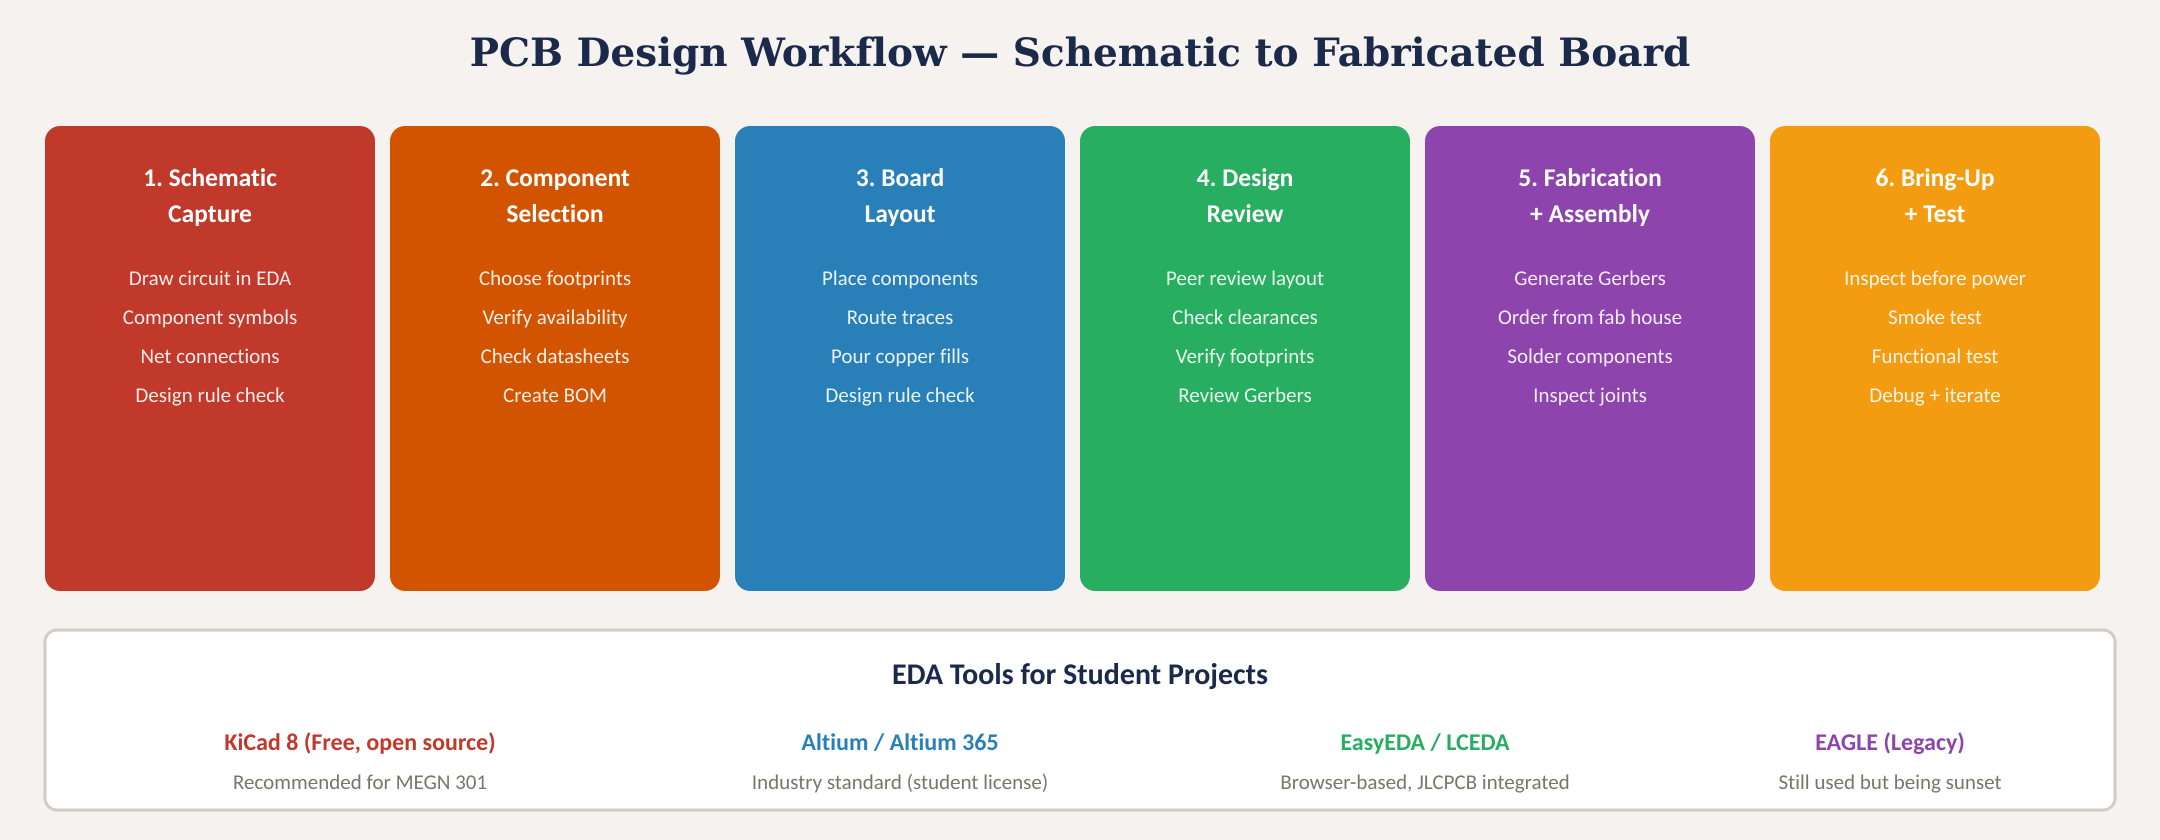
\includegraphics[width=\textwidth]{master_figs/fig_pcb_design_workflow.png}
\caption{Six-stage PCB design workflow from schematic capture through board bring-up.}\label{fig:wkfl}
\end{figure}

Six stages: (1) \textbf{Schematic capture}; draw circuit with component symbols and net connections. (2) \textbf{Component selection}; map symbols to physical footprints, verify availability, create BOM. (3) \textbf{Board layout}; place components, route traces, pour copper fills. (4) \textbf{Design review}; peer review, check clearances, verify footprints, review Gerbers. (5) \textbf{Fabrication + assembly}; generate Gerbers, order boards, solder. (6) \textbf{Bring-up + test}; inspect, smoke test, functional test, debug.

Recommended EDA tool: \textbf{KiCad 8} (free, open-source, fully capable). Alternatives: Altium (industry standard, student license), EasyEDA (browser-based, JLCPCB integrated).


\section{Schematic Capture Best Practices}

\subsection{Schematic Organization}
A professional schematic is a \emph{communication document}, not just a wiring diagram. Follow these rules from IPC-2612 [20]:
\begin{enumerate}[nosep,leftmargin=1.5em]
\item \textbf{One functional block per sheet}: power supply on Sheet~1, MCU + peripherals on Sheet~2, motor drivers on Sheet~3, connectors on Sheet~4. Title each sheet.
\item \textbf{Signal flow left to right}: inputs on the left, outputs on the right. Power flows top (VCC) to bottom (GND).
\item \textbf{Net labels over long wires}: replace wires that cross the entire sheet with named net labels (e.g., \texttt{MOTOR\_PWM}, \texttt{SDA}, \texttt{VBAT}). This eliminates spaghetti routing.
\item \textbf{Power flags}: explicitly show where power enters the schematic. Add decoupling caps adjacent to every IC symbol, not on a separate ``capacitor page.''
\item \textbf{Consistent reference designators}: R for resistors, C for capacitors, U for ICs, J for connectors, D for diodes, Q for transistors, L for inductors.
\end{enumerate}

\subsection{Component Selection and Footprint Verification}
The most expensive PCB mistake is a wrong footprint. For every component:
\begin{enumerate}[nosep,leftmargin=1.5em]
\item Download the \textbf{manufacturer's datasheet} (not a distributor summary page).
\item Find the \textbf{recommended land pattern} (footprint) in the datasheet's ``Package Information'' section.
\item Verify the KiCad library footprint dimensions match the datasheet \textbf{exactly}: pad size, pad pitch, courtyard.
\item If no library footprint exists, create one from the datasheet using KiCad's footprint editor. Measure twice.
\item \textbf{Cross-check}: print the footprint at 1:1 scale and physically place the component on the printout.
\end{enumerate}

\begin{warningbox}[The \$50 Footprint Mistake]
A team ordered 5 PCBs (\$25 total) with a QFN-32 footprint that had the wrong pad pitch (0.5\,mm vs.\ 0.65\,mm). All 5 boards were scrap. The fix required a new board spin: another \$25 + 2 weeks of lost schedule. Total cost of one unchecked footprint: \$50 + 2 weeks. The 1:1 printout would have caught this in 30 seconds.
\end{warningbox}

\subsection{Design Rule Configuration}
Configure KiCad's DRC rules before starting layout:
\begin{table}[htbp]\centering\small
\begin{tabularx}{\textwidth}{l c c X}
\toprule
\textbf{Rule} & \textbf{Minimum} & \textbf{Recommended} & \textbf{Notes} \\
\midrule
Trace width (signal) & 6\,mil & 10\,mil & Wider = easier to solder rework \\
Trace width (power) & Per IPC calc & 50--200\,mil & Size for actual current \\
Trace spacing & 6\,mil & 8\,mil & Tight spacing increases fab cost \\
Via drill & 0.3\,mm & 0.4\,mm & Smaller vias cost more \\
Via annular ring & 0.15\,mm & 0.25\,mm & Larger = more reliable \\
Clearance to edge & 0.3\,mm & 0.5\,mm & Prevents copper exposure at board edge \\
\bottomrule
\end{tabularx}
\caption{Recommended DRC rules for MEGN~301 PCBs (JLCPCB/PCBWay compatible).}
\end{table}

\section{Critical Layout Rules}

\subsection{Decoupling Capacitors}
Place a 100\,nF ceramic capacitor within 5\,mm of every IC power pin, connected with the shortest possible traces. Add one 10\,$\mu$F bulk capacitor per power rail. Via directly to ground plane for the ground side. This is not optional; without decoupling, MCUs reset and ADCs produce garbage data.

\subsection{Ground Plane}
On a 2-layer board, fill the bottom layer with a ground copper pour. This provides a low-impedance return path for all signals and dramatically reduces noise. Connect the pour to GND with abundant vias. Avoid splitting the ground plane; a split forces return current to detour.

\subsection{Component Placement and Routing}
Place components before routing. Group by function. Keep high-current paths short. Route power first, then sensitive signals, then non-critical digital. Avoid 90-degree trace corners (use 45-degree). Keep analog and digital sections physically separated. Add thermal relief pads on ground-plane connections for hand soldering.

\begin{tipbox}[The \#1 Rule]
\textbf{PRINT YOUR BOARD AT 1:1 SCALE AND PLACE REAL COMPONENTS ON THE PRINTOUT} before ordering. This single step catches 80\% of footprint errors; the most expensive PCB mistake (wrong footprint = scrap board).
\end{tipbox}

\section{Fabrication, Assembly, and Bring-Up}

\subsection{Fabrication Files}
\textbf{Gerber files} (RS-274X format): one per layer. \textbf{Drill files} (Excellon): hole coordinates and diameters. \textbf{BOM + pick-and-place}: for assembly services. Always verify in a standalone Gerber viewer before ordering.

\subsection{Fab Houses}
JLCPCB: 5 boards for \$2--7 + shipping (5--7 day fab). PCBWay: similar. OSH Park: \$5/sq-in, US-based. Order early; total timeline is 4--6 weeks from design start to working board.

\subsection{Board Bring-Up Protocol}

\begin{warningbox}[Step 1 Is Mandatory: No Exceptions]
\textbf{Do not apply power to any board until Step~1 is complete and signed off.} Skipping visual inspection is the fastest way to destroy a \$40 ESP32 module. A single solder bridge on a 0.5\,mm-pitch IC creates a dead short that damages the component the instant power is applied.
\end{warningbox}

\begin{enumerate}[leftmargin=1.5em]
\item \textbf{Visual inspection under $\geq$10$\times$ magnification} (loupe, USB microscope, or stereo microscope). This is a \textbf{mandatory gate}; a teammate must co-sign the inspection before power is applied. Inspect \emph{every} solder joint. Specific defects to look for:
\begin{itemize}[nosep,leftmargin=1.5em]
\item \textbf{Solder bridges}: look between adjacent pads on fine-pitch ICs (QFP, SOIC). A bridge shorts two pins.
\item \textbf{Cold joints}: dull, grainy, or blobby solder that did not wet the pad. These create intermittent connections.
\item \textbf{Tombstoned passives}: 0603/0805 components standing on one end (one pad soldered, one lifted).
\item \textbf{Missing components}: compare the board to the BOM and the schematic. Every refdes on the silkscreen should have a component.
\item \textbf{Wrong orientation}: check polarity marks on diodes, tantalum caps, ICs (pin 1 dot), and electrolytic caps.
\end{itemize}
\item \textbf{Continuity check}: multimeter between VCC and GND on every power rail. Any reading $<$10\,$\Omega$ indicates a short. \textbf{Do not proceed until all shorts are resolved.}
\item \textbf{Current-limited power}: set bench supply to expected voltage, current limit to 50\,mA. Apply power. If the supply immediately current-limits, there is a short. Remove power and re-inspect.
\item \textbf{Voltage verification}: measure every power rail with a multimeter. Each rail should read within $\pm$5\% of its nominal voltage.
\item \textbf{Smoke test}: increase current limit to the expected operating current. Monitor for 60 seconds. Watch for: components getting hot (touch-test cautiously), smell of burning flux or plastic, any visible smoke.
\item \textbf{Functional test}: load firmware, verify heartbeat LED, test each subsystem individually before connecting external hardware.
\end{enumerate}


\subsection{Design Review Checklist}
Before ordering PCBs, verify:
\begin{enumerate}[nosep,leftmargin=1.5em]
\item DRC (Design Rule Check) passes with zero errors and zero unreviewed warnings.
\item All footprints verified against component datasheets (not just library defaults).
\item Board outline correct with mounting holes matching the enclosure.
\item All connectors accessible and oriented correctly for cable routing.
\item Silkscreen readable (refdes near components, polarity marks on diodes/caps/ICs).
\item 1:1 printout with real components placed; \textbf{this catches 80\% of errors}.
\item Gerber files opened in a standalone viewer and visually inspected layer by layer.
\item BOM cross-checked against schematic (every schematic component in BOM and vice versa).
\item Peer review by at least one teammate who did not do the layout.
\end{enumerate}

\subsection{Development Board Integration}
When using a development board (ESP32 DevKit, Arduino Nano) instead of a custom PCB:
\begin{itemize}[nosep,leftmargin=1.5em]
\item Mount the dev board on a custom carrier PCB or perfboard with proper headers.
\item Use screw terminals or JST connectors (not breadboard jumper wires) for all permanent connections.
\item Add status LEDs and test points to the carrier board.
\item Document the wiring diagram with connector pin assignments.
\item Secure all wires with strain relief (zip ties, hot glue at connector exit points).
\end{itemize}
A well-wired development board that meets all requirements is superior to a custom PCB that delays the project or has errors.


\section{EMI, Noise, and Signal Integrity}

\subsection{The Return Current Problem}
Every signal current has a return current that flows through the ground plane (or ground trace) back to the source. The return current follows the path of \emph{least impedance}; at high frequencies, this is the path directly beneath the signal trace. If the ground plane is split or missing under a signal trace, the return current detours, creating a large loop antenna that radiates EMI and picks up noise.

\textbf{Rule}: never split the ground plane. If you must route a trace on the ground layer, stitch the ground pour back together with vias on both sides of the crossing.

\subsection{Analog-Digital Separation}
Mixed-signal boards (analog sensors + digital MCU + motor drivers) are the norm in MEGN~301 projects. Three strategies:
\begin{enumerate}[nosep,leftmargin=1.5em]
\item \textbf{Physical separation}: place analog components (sensors, ADC, analog filters) on one side of the board, digital components (MCU, motor drivers) on the other.
\item \textbf{Separate power rails}: use separate voltage regulators for analog and digital sections. At minimum, use an RC filter ($10\,\Omega + 10\,\mu$F) between the digital supply and the analog supply.
\item \textbf{Single-point ground connection}: if using split ground pours (advanced), connect them at exactly one point near the ADC. For most student projects, a single continuous ground pour with careful component placement is sufficient and safer.
\end{enumerate}

\subsection{Motor Noise Mitigation on PCB}
Motor PWM switching generates noise on every power and ground trace. Mitigation:
\begin{itemize}[nosep,leftmargin=1.5em]
\item Route motor power traces on a separate layer or board region from signal traces.
\item Place ceramic capacitors (100\,nF) directly across motor driver power pins.
\item Add a bulk electrolytic ($100$--$470\,\mu$F) at the motor power input.
\item Use a TVS diode on the motor power bus for transient suppression.
\item Never share ground vias between motor driver and MCU sections.
\end{itemize}

\section{Thermal Management on PCBs}
Components that dissipate significant power require thermal design:
\begin{itemize}[leftmargin=1.5em]
\item \textbf{Thermal pads}: many voltage regulators and motor drivers have an exposed pad on the bottom of the package. This pad \textbf{must} be soldered to a copper area on the PCB and connected to internal ground planes with thermal vias (array of 0.3\,mm vias on 1.0\,mm pitch under the pad).
\item \textbf{Copper pour as heatsink}: for SOT-223 or D-PAK regulators, extend the ground pour under and around the package. Each square centimeter of 1-oz copper on the outer layer provides approximately $60\,^{\circ}$C/W of thermal resistance to ambient.
\item \textbf{Thermal relief}: for hand-soldering, use thermal relief pads (spoke connections) on ground-connected pads. Without them, the ground plane wicks heat away faster than the soldering iron can supply it, resulting in cold joints.
\end{itemize}

\begin{tipbox}[Quick Thermal Check]
For any linear regulator: $P = (V_{in} - V_{out}) \times I_{load}$. If $P > 0.5$\,W, you need thermal analysis. If $P > 1$\,W, you probably need a switching regulator instead.
\end{tipbox}

\begin{keyconceptbox}[Requirements Mapping: From PCB Specs to Shall-Statements]
PCB design decisions directly generate system requirements:
\begin{itemize}[nosep,leftmargin=1.5em]
\item ``Board fits in 60$\times$40\,mm enclosure'' $\to$ SYS-REQ: The PCB shall have maximum dimensions of 58$\times$38\,mm with mounting holes at [coordinates].
\item ``Motor driver draws 3\,A'' $\to$ PCB-REQ: Motor power traces shall be $\geq$150\,mil wide on 1-oz copper.
\item ``ADC reads 0--3.3\,V sensors'' $\to$ PCB-REQ: Analog input traces shall be routed $\geq$10\,mm from motor power traces with a continuous ground plane beneath.
\end{itemize}
Every technical specification in Part~II should trace back to a shall-statement in your SDRD.
\end{keyconceptbox}

\section{Common Mistakes}

\begin{figure}[htbp]\centering
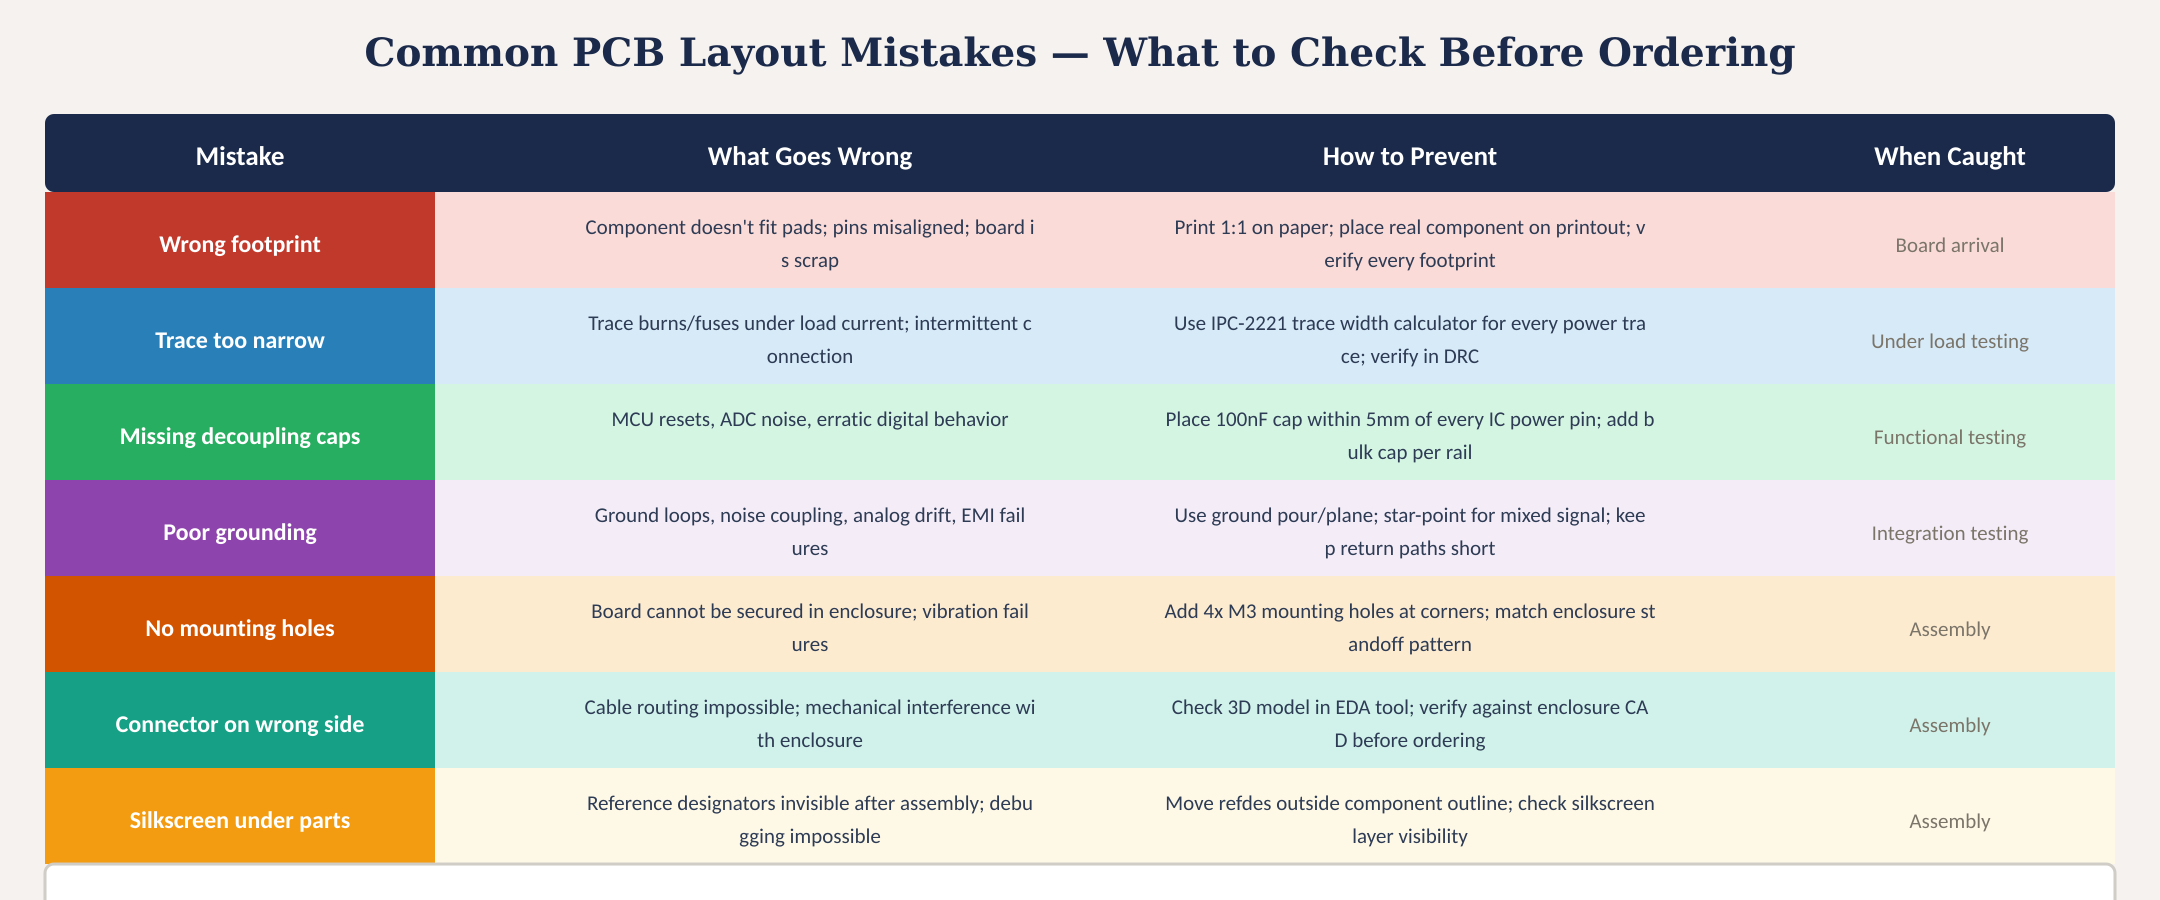
\includegraphics[width=\textwidth]{master_figs/fig_pcb_common_mistakes.png}
\caption{Seven common PCB layout mistakes with consequences and prevention strategies.}\label{fig:mistakes}
\end{figure}

Wrong footprint (scrap board), trace too narrow (burns under load), missing decoupling caps (erratic behavior), poor grounding (noise), no mounting holes (cannot secure board), connector on wrong side (cable routing impossible), silkscreen under parts (cannot read refdes). Prevention: print 1:1, run DRC, peer review, use 3D viewer.

\subsection{Development Boards vs Custom PCBs}
Use dev boards when: circuit is straightforward, form factor is not critical, timeline is tight, design is still evolving, or a suitable module already exists. Use custom PCBs when: specific form factor required, noise-sensitive analog, high reliability needed, multiple units, or clean cable routing. A well-wired dev board that meets requirements is superior to a custom PCB that delays the project.

\section{Artifact Handoff: What This Chapter Supports}
\begin{table}[htbp]\centering\small
\begin{tabularx}{\textwidth}{l X l}
\toprule
\textbf{Artifact} & \textbf{Description} & \textbf{Key Deliverable For} \\
\midrule
Schematic & Complete circuit with all component values & CDR, FDR \\
PCB Layout & Gerber files ready for fabrication & CDR (procurement) \\
BOM (electronics) & Components with package, value, vendor, Plan B & CDR, FDR \\
\bottomrule
\end{tabularx}
\end{table}

\section{PCB Design Rules for Student Projects}
\subsection{Trace Width and Current Capacity}
The PCB trace must be wide enough to carry the required current without excessive temperature rise. For external layers on 1\,oz copper (35\,$\mu$m thick):

\begin{itemize}[nosep,leftmargin=1.5em]
\item 0.25\,mm (10\,mil): 0.5\,A max (signal traces)
\item 0.5\,mm (20\,mil): 1.0\,A (low-power signals and buses)
\item 1.0\,mm (40\,mil): 2.0\,A (moderate power)
\item 2.5\,mm (100\,mil): 4.0\,A (motor drivers, heater connections)
\item 5.0\,mm (200\,mil): 7.0\,A (high-current power)
\end{itemize}

These values assume 10\,\degC{} temperature rise above ambient. For buried (internal) layers: derate by 50\%. For 2\,oz copper: multiply current capacity by $\sqrt{2} \approx 1.4$.

\subsection{Clearance and Creepage}
\textbf{Clearance}: the shortest distance through air between two conductors. For circuits under 50\,V: minimum 0.25\,mm (10\,mil). For 50--300\,V: minimum 1.5\,mm.

\textbf{Creepage}: the shortest distance along a surface between two conductors. Creepage must be larger than clearance because surface contamination (dust, flux residue, moisture) reduces the breakdown voltage. For circuits under 50\,V: minimum 0.5\,mm. For mains-connected circuits: consult IPC-2221 or the relevant safety standard.

\subsection{Via Design}
Vias connect traces between layers. For signal vias: 0.3\,mm drill, 0.6\,mm pad. For power vias: 0.4\,mm drill, 0.8\,mm pad, or use multiple vias in parallel for high current. Thermal vias under power components (voltage regulators, MOSFETs) connect the component pad to internal or bottom copper planes for heat dissipation. Use a grid of 4--9 vias with 0.3\,mm drill directly under the thermal pad.

\section{Component Placement Strategy}
Good placement is 80\% of good PCB design. Follow this sequence:

(1) \textbf{Place connectors first}: power input, signal I/O, programming header. These have fixed locations (edge of board, near panel cutouts). All other placement works around them.

(2) \textbf{Place the MCU}: central location, near the programming header. Orient so that bus signals (SPI, I2C, UART) route cleanly to their destinations.

(3) \textbf{Place power components}: voltage regulator near the power input connector. Input capacitor between the regulator and connector. Output capacitor between the regulator and the MCU. Keep the power path short and wide.

(4) \textbf{Place analog components}: sensors, amplifiers, ADCs as far as possible from switching noise sources (voltage regulators, motor drivers, digital buses). Ideally on the opposite side of the board or in a separate analog ground island.

(5) \textbf{Place remaining digital components}: group by function (communication, display, storage). Keep I2C devices on a clean bus with short traces.

\section{Design Review Before Fabrication}
Before submitting the PCB for fabrication, perform a systematic review:

\textbf{Schematic review}: verify every net is connected as intended. Check power and ground connections for every IC. Verify component values match the design calculations.

\textbf{Layout review}: run the DRC (Design Rule Check) and fix all violations. Visually inspect: are all traces routed? Are power traces wide enough? Are decoupling capacitors close to their ICs? Is there adequate clearance around mounting holes?

\textbf{3D review}: if the EDA tool supports 3D rendering (KiCad, Altium), verify that components do not interfere with the enclosure, connectors are accessible, and tall components do not block test points.

\textbf{Fabrication files}: generate Gerber files and the drill file. Open them in a Gerber viewer (KiCad's built-in viewer, or the fab house's online viewer) and verify that the actual output matches the design. Check that the board outline, mounting holes, and silkscreen are correct.
\begin{warningbox}[Mandatory: 10$\times$ Visual Inspection Before Power-On]
Before applying power to any newly assembled PCB, perform a visual inspection under at least 10$\times$ magnification (jeweler's loupe, USB microscope, or stereo microscope). Inspect every solder joint for:

\textbf{Solder bridges}: unintended connections between adjacent pads, especially on fine-pitch ICs (0.5\,mm pitch QFP, 0.65\,mm SOIC). A single bridge between V$_{\text{CC}}$ and an I/O pin will destroy the IC at power-on.

\textbf{Cold joints}: dull, grainy, or blobby joints that did not wet properly. These create intermittent connections that work on the bench but fail under vibration.

\textbf{Tombstoned components}: 0402 and 0603 passives that lifted on one end during reflow, creating an open circuit. The component stands vertically like a tombstone.

\textbf{Missing components}: compare the board to the BOM and assembly drawing. A missing decoupling capacitor can cause oscillation; a missing pull-up resistor can hang the I2C bus.

\textbf{Polarity}: verify orientation of every polarized component (electrolytic capacitors, diodes, ICs, connectors). A reversed electrolytic capacitor will explode within seconds of power-on.

This inspection is a \textbf{gate}: no power is applied until a second team member has signed off on the visual inspection. This 5-minute check prevents the most common cause of PCB failure in student projects: immediate destruction of components due to assembly errors that were visible but unchecked.
\end{warningbox}
\section{Practice Questions}
\begin{enumerate}[leftmargin=1.5em]
\item Your project has a motor driver that draws 3\,A peak. What is the minimum trace width for the motor power traces on a 2-layer board with 1-oz external copper? What width would you actually use and why?
\item A teammate's PCB layout has the 100\,nF decoupling capacitors placed 25\,mm from the MCU power pins ``because there was more room over there.'' Explain why this is a problem and what the correct placement is.
\item You receive your first PCB from JLCPCB. Describe the exact sequence of steps you follow before connecting the board to your system.
\item Your team is debating whether to design a custom PCB or use an Arduino Nano + sensor breakout boards. The project is a battery-powered environmental monitor that must fit inside a 60$\times$40$\times$25\,mm waterproof enclosure. Argue for or against a custom PCB with specific reasoning.
\item A 2-layer board has all signal traces on the top layer and a ground pour on the bottom. A teammate routes a high-current motor trace on the bottom layer, cutting through the ground pour. What problems will this cause and how should it be fixed?
\item Your schematic uses an LM1117-3.3 voltage regulator in an SOT-223 package to power an ESP32. The datasheet shows a thermal pad on the bottom. Your PCB layout connects the thermal pad to a small isolated copper island with no vias. Calculate the power dissipation at 5\,V input, 3.3\,V output, 300\,mA load, and explain why the current thermal design is inadequate.
\item You are designing a mixed-signal board with a 12-bit ADC reading a strain gauge (millivolt-level signal) and an H-bridge motor driver on the same PCB. Describe three specific layout strategies to prevent motor noise from corrupting the ADC readings.
\item Your team's KiCad DRC reports 47 ``courtyard overlap'' warnings. Your teammate dismisses them: ``It compiles fine, just ignore warnings.'' Explain why courtyard overlaps are serious and what physical problem they represent.
\end{enumerate}

\subsection{Answers}
\begin{enumerate}[leftmargin=1.5em]
\item From the IPC-2221 reference: 3\,A on 1-oz external copper requires approximately 100\,mil (2.5\,mm) trace width. In practice, use 150--200\,mil (3.8--5\,mm) to provide thermal margin, reduce voltage drop, and account for peak transients. Always add margin on power traces; the cost is board space, not money.
\item At 25\,mm, the trace inductance between the cap and the IC power pin negates the decoupling effect. High-frequency noise (MHz range) sees the inductance as a high impedance and is not filtered. The cap must be within 5\,mm with the shortest possible traces and a via directly to the ground plane. The loop area (VCC pin $\to$ cap $\to$ GND via $\to$ GND plane $\to$ IC GND pin) must be minimized.
\item Follow the six-step bring-up protocol: (1) Visual inspection under magnification for bridges, cold joints, and wrong-orientation parts. (2) Multimeter continuity check for VCC-to-GND shorts. (3) Current-limited bench supply at 50\,mA, apply expected voltage. (4) Measure all power rails with multimeter. (5) Increase current limit to operating level, monitor 60 seconds for heat/smell. (6) Load firmware, test basic I/O.
\item Argue FOR custom PCB: the 60$\times$40$\times$25\,mm enclosure is too small for an Arduino Nano (45$\times$18\,mm) plus breakout boards plus wiring. A custom board can integrate the MCU, sensors, and battery management into the available footprint with board-edge connectors for waterproof cable glands. The waterproof requirement also favors a single board with conformal coating over loose wiring that can vibrate and corrode. However: this requires the design to be frozen by CDR and 4--6 weeks of lead time.
\item The motor trace cuts the ground pour, forcing signal return currents to detour around the gap. This creates a large current loop that radiates EMI and couples noise into adjacent signal traces. The motor's switching noise (from PWM) will appear as voltage spikes on the ground plane near the gap, potentially corrupting ADC readings and causing MCU resets. Fix: route the motor power traces on the top layer using wide traces, keeping the bottom ground pour continuous. If the motor trace must cross to the bottom, use a narrow bridge with ground pour restored on both sides and stitching vias.
\item $P = (5.0 - 3.3) \times 0.3 = 0.51$\,W. SOT-223 $\theta_{JA}$ without thermal vias $\approx 150$\,\degC{}/W, so $\Delta T = 76.5$\,\degC{}. At 25\,\degC{} ambient: $T_J = 101.5$\,\degC{}, approaching the 125\,\degC{} limit. At 40\,\degC{} ambient (inside an enclosure): $T_J = 116.5$\,\degC{}, dangerous. The isolated copper island with no vias provides poor thermal coupling to inner layers. Fix: add an array of thermal vias (5--9 vias, 0.3\,mm drill, 1.0\,mm pitch) under the thermal pad, connecting to the ground plane on Layer~2. This reduces $\theta_{JA}$ to $\sim$60\,\degC{}/W.
\item (1) Physical separation: place ADC and strain gauge conditioning on the left half of the board, motor driver on the right, with a clear ``quiet zone'' boundary between them. (2) Separate analog supply: use an RC filter (10\,$\Omega$ + 10\,$\mu$F) between digital VCC and the ADC's AVCC pin to prevent motor switching noise from reaching the analog reference. (3) Guard ring/trace: surround the strain gauge signal traces with a grounded guard trace connected to the analog ground, shielding them from electric field coupling. Additionally: route motor power traces perpendicular (not parallel) to analog signal traces when crossings are unavoidable.
\item Courtyard overlaps mean two components occupy the same physical space on the board. They will either mechanically interfere (components crash into each other during assembly), or their solder pads will short together. DRC warnings are not cosmetic; they represent physical manufacturing problems. Fix: move one component until courtyards no longer overlap. If space is genuinely tight, verify in the 3D viewer that the components physically clear each other.
\end{enumerate}


\chapter{Microcontrollers \& the ESP32}

\vspace{1em}


\vspace{1em}

\section{MCU Fundamentals}
\subsection{What Is a Microcontroller?}
A microcontroller (MCU) integrates a CPU, memory (flash + SRAM), and peripherals (GPIO, ADC, timers, communication) on a single chip. Unlike a microprocessor (Raspberry Pi), an MCU requires no external RAM or storage; it is self-contained and runs bare-metal or RTOS code.

\textbf{Key blocks}: CPU core (executes instructions, 16--600\,MHz), flash memory (stores program, 32\,KB--16\,MB), SRAM (runtime variables, 2\,KB--520\,KB), peripherals (GPIO, ADC, DAC, PWM, timers, watchdog, RTC), communication (UART, SPI, I2C, CAN, Wi-Fi, BLE), and power management (regulators, sleep modes, brown-out detect).

\begin{figure}[htbp]\centering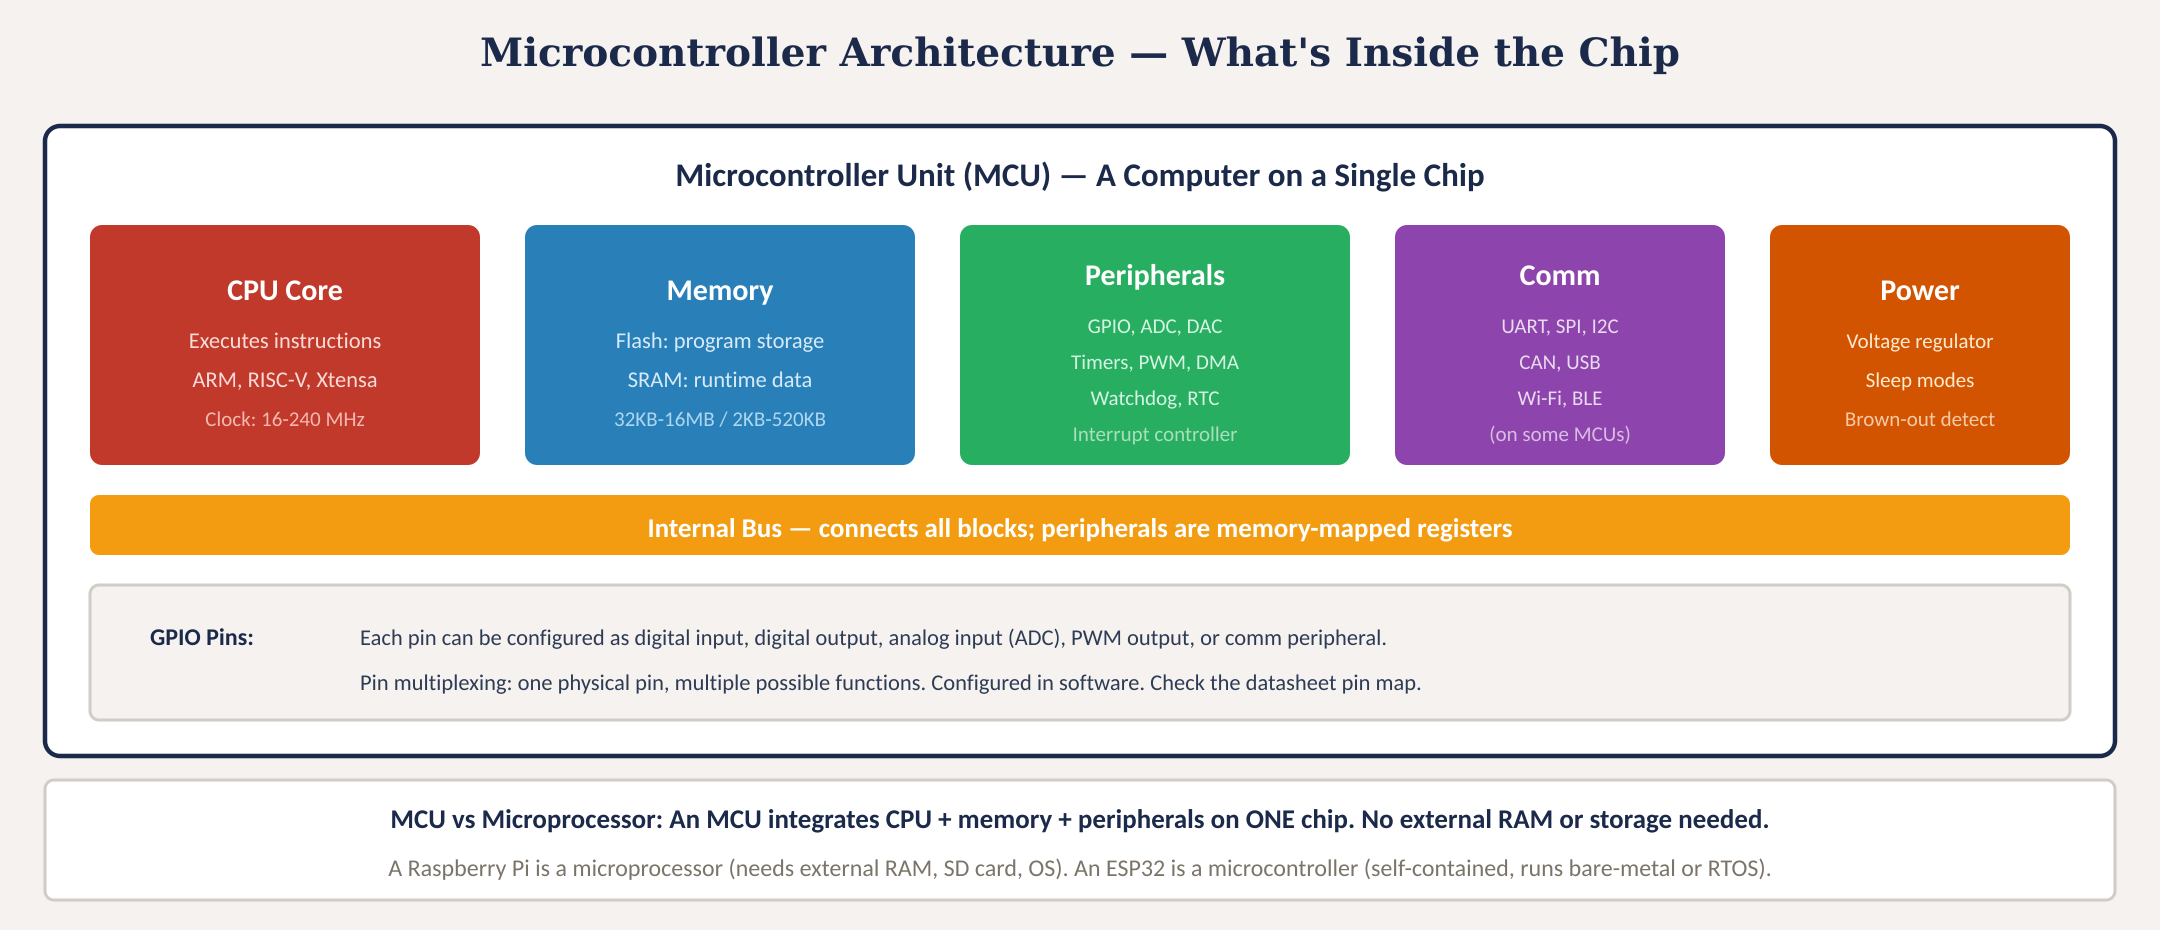
\includegraphics[width=\textwidth]{master_figs/fig_mcu_architecture.png}
\caption{MCU internal architecture: CPU, memory, peripherals, communication, and power on one chip.}\end{figure}

\subsection{MCU Platform Comparison}
\begin{figure}[htbp]\centering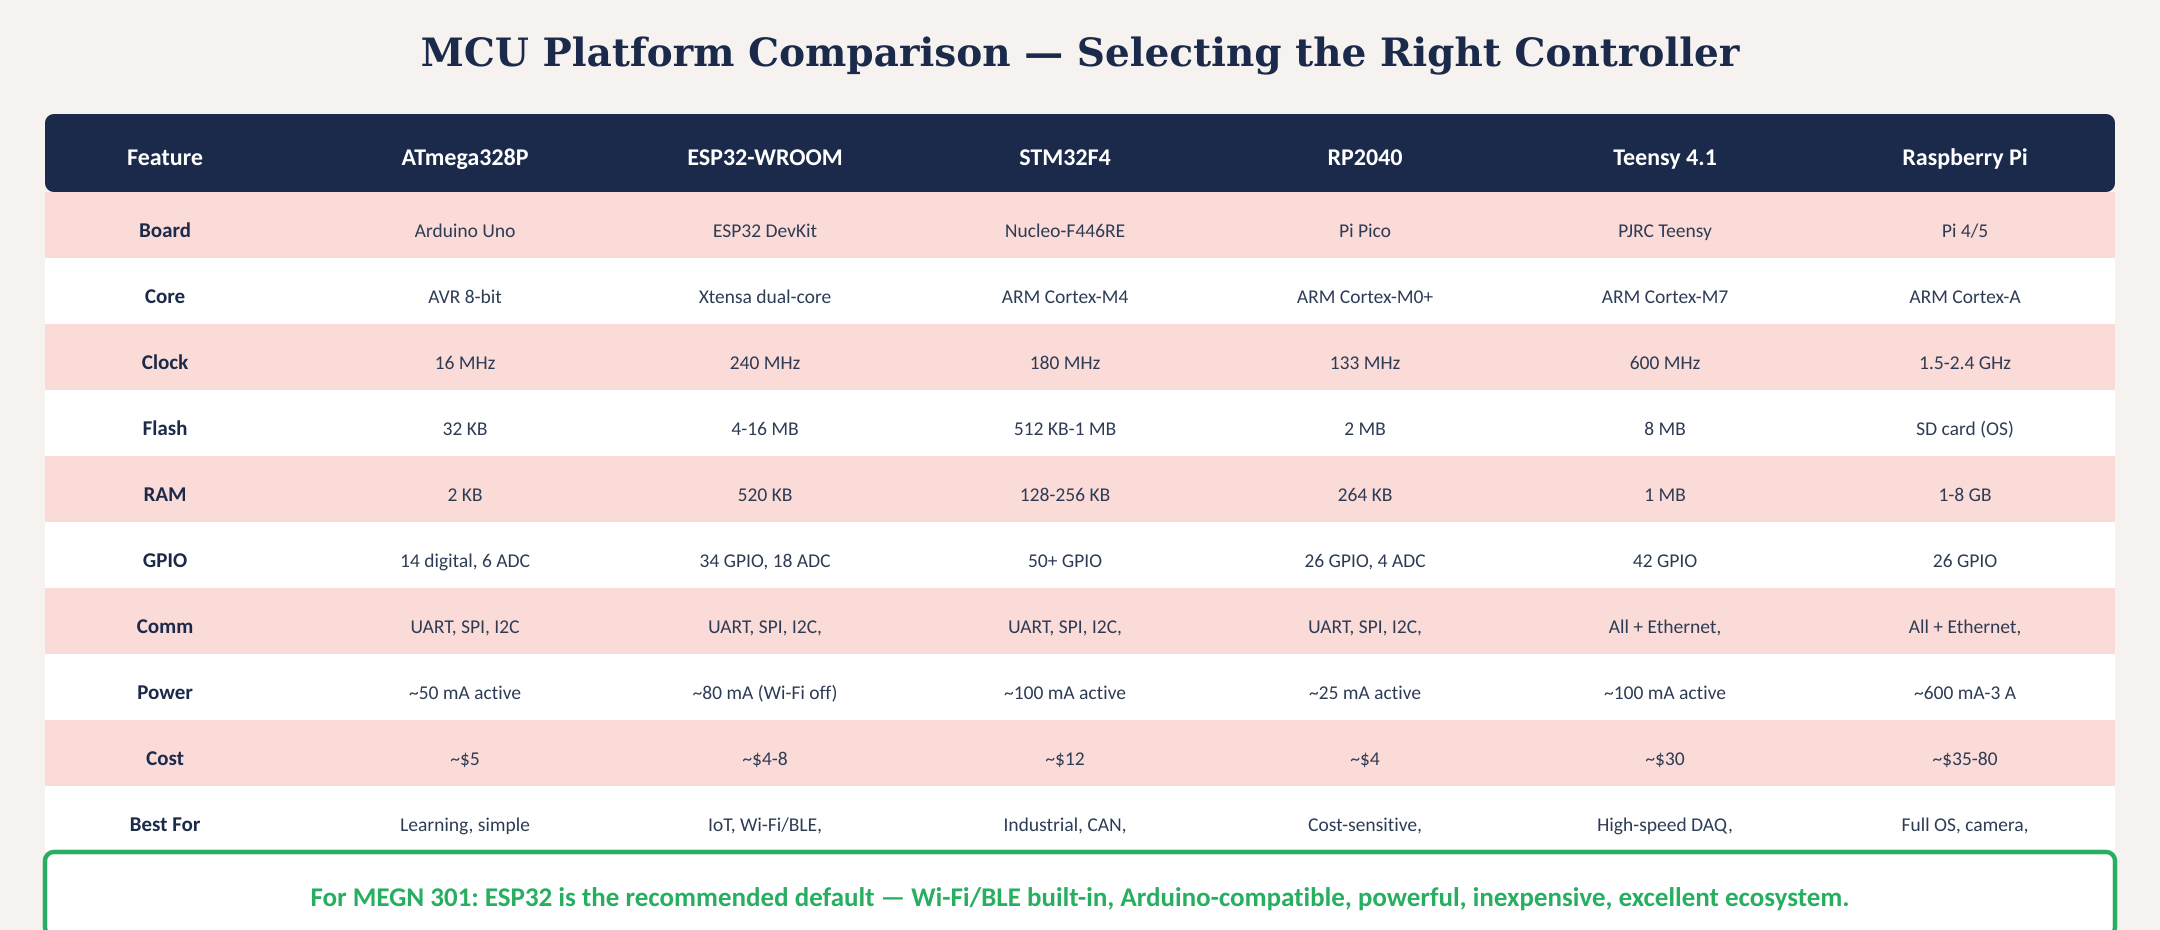
\includegraphics[width=\textwidth]{master_figs/fig_mcu_comparison.png}
\caption{Six MCU platforms compared. ESP32 recommended for MEGN 301.}\end{figure}

\textbf{Selection criteria}: GPIO count (add 20\% margin), communication protocols needed, processing power, power budget (deep sleep current for battery), ecosystem (libraries, community), and cost/availability.

\section{ESP32 Deep Dive}
The ESP32-WROOM-32 is the recommended MCU for MEGN 301 projects: dual-core Xtensa LX6 at 240\,MHz, 520\,KB SRAM, 4\,MB flash, built-in Wi-Fi (802.11 b/g/n) and Bluetooth (Classic + BLE 4.2), 34 GPIO, 18 ADC channels (12-bit), 2 DAC channels (8-bit), 16 PWM channels, 3 UART, 2 SPI, 2 I2C, 1 CAN, 10 capacitive touch pins, deep sleep at $\$\sim\$$10\,$\mu$A. Cost: \$4--8 for a DevKit board.

\begin{figure}[htbp]\centering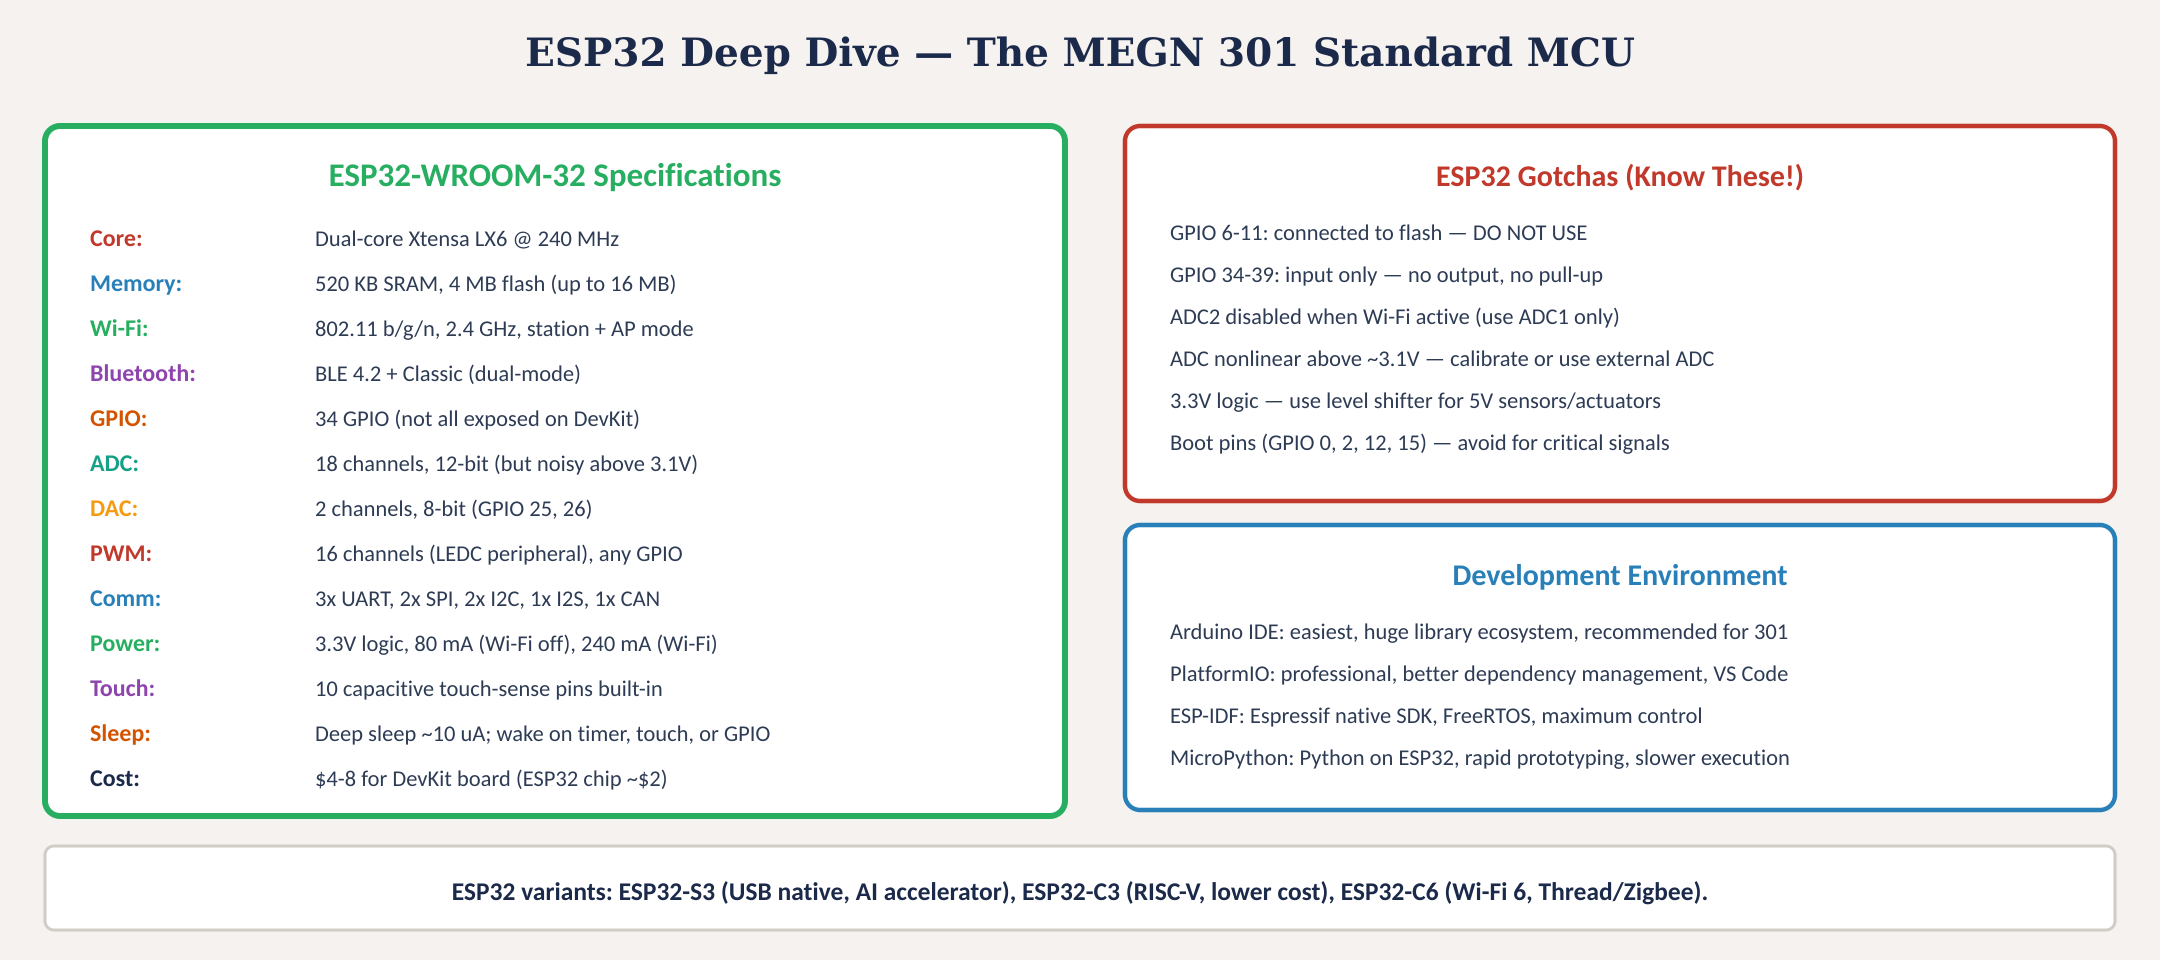
\includegraphics[width=\textwidth]{master_figs/fig_esp32_deep_dive.png}
\caption{ESP32 specifications, gotchas, and development environment.}\end{figure}

\begin{warningbox}[ESP32 Gotchas: Memorize These]
\begin{itemize}[nosep,leftmargin=1.5em]
\item \textbf{GPIO 6--11}: connected to internal flash. DO NOT USE.
\item \textbf{GPIO 34--39}: input only; no output, no internal pull-up.
\item \textbf{ADC2 disabled when Wi-Fi active}: use ADC1 (GPIO 32--39) only.
\item \textbf{ADC nonlinear above $\$\sim\$$3.1\,V}: calibrate or use external ADC for precision.
\item \textbf{3.3\,V logic}: use level shifters for 5\,V sensors/actuators.
\item \textbf{Boot pins (0, 2, 12, 15)}: avoid for critical signals; unexpected levels prevent boot.
\end{itemize}
\end{warningbox}

\subsection{Safe GPIO Selection}
\textbf{Safe for any use}: GPIO 4, 13, 14, 16--19, 21--23, 25--27, 32, 33. \textbf{Input only}: GPIO 34, 35, 36 (VP), 39 (VN). \textbf{Boot-sensitive}: GPIO 0, 2, 12, 15 (usable after boot with care). \textbf{Off-limits}: GPIO 6--11 (flash), 1 (TX0), 3 (RX0).

\subsection{Wi-Fi and Bluetooth}
\textbf{Wi-Fi}: Station mode (connect to router), AP mode (create network), or both. ESP-NOW for peer-to-peer without router. \textbf{BLE}: GATT server/client for phone apps; lower power than Classic BT. \textbf{Classic BT}: Serial Port Profile for wireless UART.

\subsection{Power Modes}
Active ($\$\sim\$$240\,mA with Wi-Fi), modem sleep ($\$\sim\$$20\,mA, radio off), light sleep ($\$\sim\$$0.8\,mA, CPU paused), deep sleep ($\$\sim\$$10\,$\mu$A, RTC only). Battery sizing example: 2000\,mAh LiPo at active+Wi-Fi = 10 hours; at deep sleep with 1-min wakeups ($\$\sim\$$0.5\,mA average) = 166 days.

\section{Communication Protocols}
\begin{figure}[htbp]\centering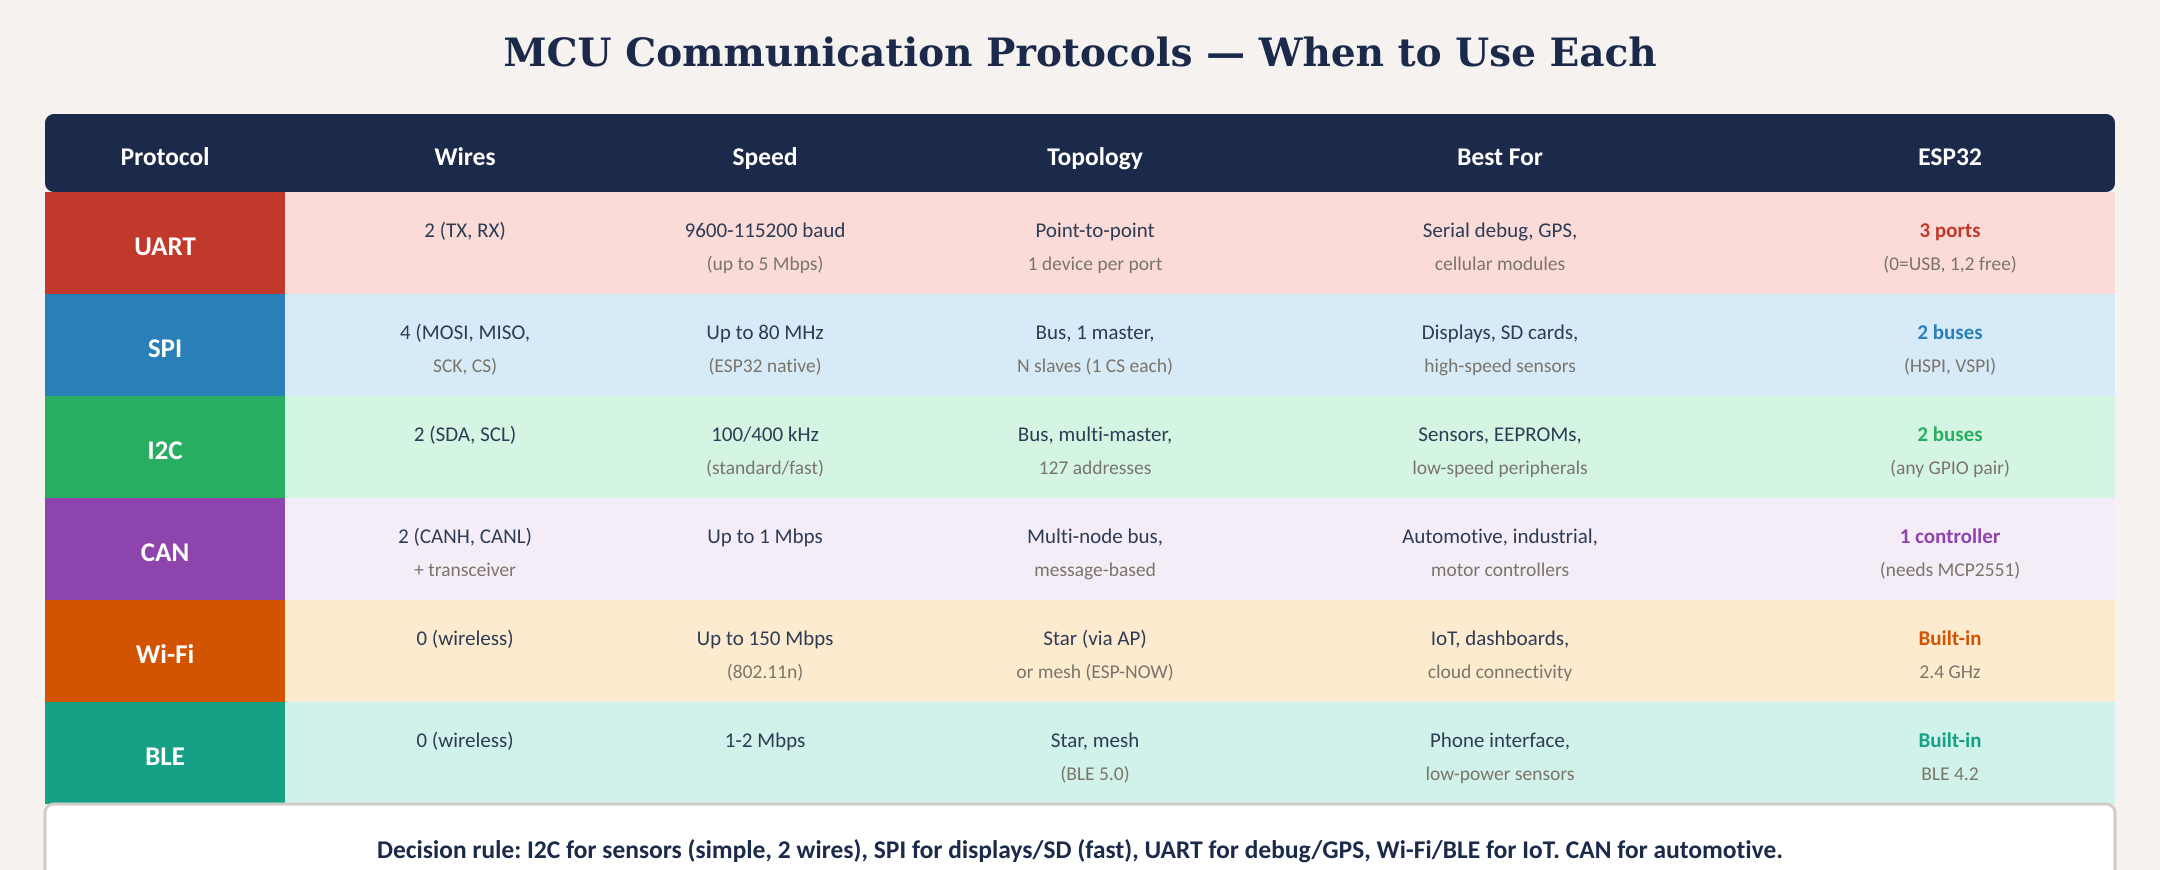
\includegraphics[width=\textwidth]{master_figs/fig_mcu_protocols.png}
\caption{Six communication protocols with wire count, speed, topology, and ESP32 support.}\end{figure}

\textbf{UART}: 2 wires, point-to-point, 9600--115200 baud. Debug, GPS, cellular. \textbf{SPI}: 4 wires + CS, bus, up to 80\,MHz. Displays, SD cards, fast sensors. \textbf{I2C}: 2 wires, bus, 100--400\,kHz, 127 addresses. Most sensors (BME280, MPU6050). Needs 4.7\,k$\Omega$ pull-ups. \textbf{CAN}: 2 wires + transceiver, multi-node, 1\,Mbps. Automotive/industrial. \textbf{Wi-Fi/BLE}: wireless IoT.

\begin{tipbox}[Protocol Decision Rule]
I2C for sensors (simple, 2 wires). SPI for displays and SD cards (fast). UART for debug and GPS. Wi-Fi/BLE for IoT connectivity. CAN for automotive.
\end{tipbox}

\section{Firmware and Integration}
\subsection{Firmware Best Practices}
Use \textbf{state machines} (IDLE, READING, TRANSMITTING, SLEEPING). Use \texttt{millis()}-based timing instead of \texttt{delay()}. Use \textbf{interrupts} for hardware events (ISRs must be short; set a flag, process in loop). Enable the \textbf{watchdog timer} for crash recovery. Add a \textbf{heartbeat LED} as a health indicator.

\subsection{System Integration}
\textbf{Power}: 3.3\,V regulated or 5\,V via USB DevKit. Add 10\,$\mu$F + 100\,nF decoupling at MCU power pins. Wi-Fi transmit draws 240\,mA transient; inadequate decoupling causes brown-out resets. \textbf{Level shifting}: BSS138-based modules for I2C/SPI to 5\,V devices. \textbf{I2C}: 4.7\,k$\Omega$ pull-ups to 3.3\,V. \textbf{Analog}: keep wires short, average readings for noise reduction.

\section{Artifact Handoff: What This Chapter Supports}
\begin{table}[htbp]\centering\small
\begin{tabularx}{\textwidth}{l X l}
\toprule
\textbf{Artifact} & \textbf{Description} & \textbf{Key Deliverable For} \\
\midrule
Pin Map & GPIO assignments with function and component & CDR, FDR \\
Firmware Architecture & State machine, ISRs, communication protocols & CDR, FDR \\
Power Mode Plan & Active/sleep duty cycle for battery sizing & CDR (power budget) \\
\bottomrule
\end{tabularx}
\end{table}


\subsection{Development Environment Setup}
\textbf{Arduino IDE} (recommended for MEGN~301): Install Arduino IDE 2.x, add ESP32 board support via Board Manager\footnote{Board Manager URL: \url{https://espressif.github.io/arduino-esp32/package_esp32_index.json}}, select ``ESP32 Dev Module,'' and verify with the Blink example. \textbf{PlatformIO}: more professional, supports version-pinned dependencies and multi-file projects. \textbf{ESP-IDF}: Espressif's native framework; most powerful but steepest learning curve.

\subsection{Common Integration Patterns}
\begin{itemize}[leftmargin=1.5em]
\item \textbf{Sensor polling loop}: read all sensors in \texttt{loop()}, average 3--5 readings, apply calibration, publish to cloud/display. Use \texttt{millis()}-based timing, never \texttt{delay()}.
\item \textbf{Actuator control}: state machine with IDLE, HEATING, COOLING, FAULT states. Transitions triggered by sensor thresholds with hysteresis (e.g., turn on at 3\,\degC{}, turn off at 5\,\degC{} to prevent relay chatter).
\item \textbf{Data logging}: write sensor data to SPIFFS/LittleFS with timestamps. Upload batch to cloud on Wi-Fi schedule. Buffer locally if Wi-Fi is unavailable.
\item \textbf{OTA updates}: enable ArduinoOTA for wireless firmware updates during development. Disable in production firmware for security.
\end{itemize}

\subsection{Battery Sizing Worked Example}
GreenShield off-grid: ESP32 wakes every 60\,s for 2\,s of active measurement (80\,mA average during wake, 10\,$\mu$A during sleep). Average current:
\begin{equation}
I_{avg} = \frac{2 \times 80 + 58 \times 0.01}{60} = 2.68\,\text{mA}
\end{equation}
With a 3000\,mAh LiPo: runtime = 3000/2.68 = 1119 hours = 46 days. Adding Wi-Fi transmit (240\,mA for 1\,s every 5 minutes): adds 0.80\,mA average, total 3.48\,mA, runtime = 36 days. Add 30\% margin for battery aging: design for 25 days between charges.


\section{Sensor Interfacing Patterns}

\subsection{Analog Sensors}
Most analog sensors output a voltage proportional to the measured quantity. The ESP32's 12-bit ADC maps 0--3.3\,V to 0--4095 counts. Conversion: $V = \text{count} \times 3.3 / 4095$. Then apply the sensor's transfer function (from datasheet) to convert voltage to engineering units.

\textbf{Common problems and fixes}:
\begin{itemize}[nosep,leftmargin=1.5em]
\item \textbf{Noise}: average 10--50 readings per sample. Use a moving average or median filter in firmware.
\item \textbf{Nonlinearity}: the ESP32 ADC is nonlinear above $\sim$3.1\,V. Use the ESP-IDF calibration API (\texttt{esp\_adc\_cal}) or limit input range to 0--3.0\,V with a voltage divider.
\item \textbf{Offset/gain error}: calibrate against a known reference (multimeter) at two points and apply linear correction: $V_{true} = a \times V_{raw} + b$.
\item \textbf{5\,V sensors}: use a voltage divider or external ADC (ADS1115, 16-bit, I2C, \$3).
\end{itemize}

\subsection{Digital Sensors (I2C)}
Most modern sensors (temperature, humidity, IMU, pressure) use I2C. Basic integration:
\begin{enumerate}[nosep,leftmargin=1.5em]
\item Connect SDA to GPIO~21, SCL to GPIO~22 (ESP32 defaults).
\item Add 4.7\,k$\Omega$ pull-up resistors from SDA and SCL to 3.3\,V. \textbf{One pair per bus}, not per device.
\item Install the sensor's Arduino library via Library Manager.
\item Initialize with \texttt{Wire.begin()} and use the library's \texttt{.read()} methods.
\item If the sensor is not detected: check wiring, verify address with an I2C scanner sketch, check pull-ups with a multimeter (SDA/SCL should read 3.3\,V when idle).
\end{enumerate}

\subsection{Motor and Actuator Control}
\textbf{DC motors}: use \texttt{ledcSetup()} and \texttt{ledcWrite()} for hardware PWM at 20--25\,kHz (above audible range). Never drive a motor directly from a GPIO pin. Always use a driver IC (L298N, BTS7960, DRV8871) or MOSFET with flyback diode.

\textbf{Servo motors}: use the ESP32Servo library. Attach to any PWM-capable GPIO. Standard range: 500--2400\,$\mu$s pulse width at 50\,Hz. Power servos from a separate 5--6\,V supply, not from the ESP32's 3.3\,V rail.

\textbf{Relay control}: drive a relay module's signal input from a GPIO through a 1\,k$\Omega$ resistor. Use optocoupled relay modules to isolate the MCU from relay coil transients.

\section{Debugging and Troubleshooting}

\subsection{Serial Monitor Debugging}
\texttt{Serial.println()} is the primary debugging tool. Best practices:
\begin{itemize}[nosep,leftmargin=1.5em]
\item Print sensor values with labels: \texttt{Serial.print("Temp: "); Serial.println(temp);}
\item Add state machine transitions: \texttt{Serial.println("STATE: HEATING");}
\item Print timestamps: \texttt{Serial.print(millis()); Serial.print(" ms: ");}
\item Remove or conditionally compile debug prints before final deployment (\texttt{\#define DEBUG}).
\end{itemize}

\subsection{Common ESP32 Failure Modes}
\begin{table}[htbp]\centering\small
\begin{tabularx}{\textwidth}{l X X}
\toprule
\textbf{Symptom} & \textbf{Likely Cause} & \textbf{Fix} \\
\midrule
Random resets & Brown-out (insufficient decoupling) & Add 100\,$\mu$F + 100\,nF at regulator output \\
Won't boot & GPIO 0/2/12/15 held at wrong level & Disconnect boot-sensitive pins during upload \\
ADC reads garbage & ADC2 + Wi-Fi conflict, or input $>$3.3\,V & Use ADC1 channels; add voltage divider \\
I2C not detected & Missing pull-ups, wrong address, SDA/SCL swapped & Check with I2C scanner; verify pull-ups \\
Wi-Fi disconnects & Antenna blocked by ground plane or metal & Keep antenna area clear of copper pour \\
Servo jitter & Shared power supply with MCU & Use separate servo power supply \\
\bottomrule
\end{tabularx}
\caption{Common ESP32 failure modes, causes, and fixes.}
\end{table}

\begin{keyconceptbox}[Requirements Mapping: From MCU Specs to Shall-Statements]
MCU capabilities generate system requirements:
\begin{itemize}[nosep,leftmargin=1.5em]
\item ``Read 4 analog sensors'' $\to$ SYS-REQ: The system shall acquire analog data from 4 channels at $\geq$10\,Hz using ADC1 (GPIO 32--35).
\item ``Wireless data logging'' $\to$ SYS-REQ: The system shall transmit sensor data to a cloud server via Wi-Fi at $\geq$1 upload per 5 minutes.
\item ``Battery operation for 30 days'' $\to$ SYS-REQ: The system shall operate from a 3000\,mAh LiPo for $\geq$30 days with a duty cycle of 2\,s active per 60\,s.
\end{itemize}
The battery sizing calculation in this chapter directly verifies the last requirement. Every MCU design choice must trace to a shall-statement.
\end{keyconceptbox}

\section{Microcontroller Fundamentals}
A microcontroller (MCU) is a complete computer on a single chip: processor (CPU), memory (RAM and flash), input/output peripherals, and communication interfaces. Unlike a desktop CPU (which requires external memory, storage, and I/O), the MCU is self-contained and designed for embedded applications where cost, power, and size are constrained.

\subsection{Key Specifications}
\textbf{Clock speed}: determines the instruction execution rate. The ESP32 runs at 240\,MHz (dual core), executing $\sim$240 million simple instructions per second. This is more than adequate for control loops running at 1\,kHz, sensor acquisition, and display updates.

\textbf{Memory}: RAM stores runtime variables (sensor readings, control states, buffers). Flash stores the program (firmware) and constants (calibration tables). The ESP32 has 520\,kB RAM and 4\,MB flash, sufficient for most MEGN~301 projects. If you run out of RAM: optimize data structures, reduce buffer sizes, or use external SPI RAM.

\textbf{GPIO (General Purpose I/O)}: pins that can be configured as digital input, digital output, analog input (ADC), PWM output, or communication interface. The ESP32 has 34 GPIO pins, though some have restrictions (input-only, strapping pins, occupied by flash interface).

\textbf{ADC}: the ESP32's internal ADC is 12-bit with significant nonlinearity and noise ($\pm$50\,LSB at 12-bit). For precision measurement: use an external ADC (ADS1115: 16-bit, I2C, \$3) or the NI~DAQ. The internal ADC is adequate for: battery voltage monitoring, potentiometer reading, and coarse sensor measurement where $\pm$5\% accuracy suffices.

\textbf{Communication interfaces}: UART (serial: 3 ports), SPI (high-speed: 2 ports), I2C (moderate speed: 1 port, expandable). WiFi (802.11b/g/n) and Bluetooth (Classic + BLE) are built-in, enabling wireless data logging, remote monitoring, and over-the-air firmware updates.

\section{ESP32 Pin Planning}
Before writing code, create a pin assignment table mapping every signal to a specific GPIO pin. Constraints to observe:

GPIO 0, 2, 5, 12, 15: strapping pins that affect boot mode. Avoid using for general I/O unless you understand the boot-time implications.

GPIO 34--39: input only (no output capability). Use for analog inputs or digital inputs only.

GPIO 6--11: connected to the internal flash. Do not use.

ADC2 (GPIO 0, 2, 4, 12--15, 25--27): cannot be used for ADC while WiFi is active. Use ADC1 (GPIO 32--39) for analog inputs in WiFi-enabled projects.

\section{Firmware Architecture for Control Systems}
\subsection{Superloop Architecture}
The simplest firmware structure: a single infinite loop that reads sensors, computes control, writes actuators, and updates the display, repeating at a fixed rate:

\begin{verbatim}
void loop() {
  read_sensors();
  compute_pid();
  write_actuators();
  update_display();
  delay_until_next_period();
}
\end{verbatim}

The superloop is adequate for single-rate systems with modest complexity. It fails when: (1) the loop takes longer than the control period (timing violation), (2) different tasks need different rates (sensor at 100\,Hz, display at 10\,Hz, logging at 1\,Hz), or (3) blocking operations (WiFi, SD card write) stall the control loop.

\subsection{Task-Based Architecture (FreeRTOS)}
The ESP32 includes FreeRTOS, a real-time operating system that runs multiple tasks concurrently with priority-based scheduling. Each task has its own stack and runs as if it were the only program. The RTOS scheduler switches between tasks automatically:

High priority: control loop (reads sensor, computes PID, writes actuator). Runs every 10\,ms without interruption.

Medium priority: data logging (writes to SD card). Runs every 1\,s; may be interrupted by the control task.

Low priority: display update and WiFi communication. Runs when higher-priority tasks are idle.

This ensures the control loop always meets its timing deadline, even when lower-priority tasks are slow.

\section{Common ESP32 Pitfalls in MEGN 301}
(1) \textbf{Watchdog timer resets}: the ESP32's watchdog timer resets the system if the main loop (or a FreeRTOS task) does not yield within $\sim$3\,s. Long operations (SD card initialization, WiFi connection) trigger the watchdog. Solution: call \texttt{yield()} or \texttt{vTaskDelay(1)} inside long operations.

(2) \textbf{Power supply noise}: the ESP32's WiFi transmitter draws 120--240\,mA current pulses that cause voltage sag on weak supplies. Symptoms: random resets, ADC reading spikes, WiFi disconnections. Solution: use a dedicated 5\,V supply with $\geq$1\,A capacity and place a 470\,$\mu$F capacitor at the ESP32's 3.3\,V input.

(3) \textbf{GPIO conflicts}: accidentally configuring a strapping pin as output, or using an ADC2 pin while WiFi is active. Symptoms: boot failure, garbage ADC readings. Solution: always check the pin assignment table and the ESP32 datasheet before committing to a pin map.

(4) \textbf{Floating inputs}: unconnected GPIO pins read random noise. If your code checks a button on an unconnected pin, it sees phantom presses. Solution: enable internal pull-up or pull-down resistors on all input pins, or connect external pull-ups/pull-downs.
\begin{keyconceptbox}[Requirements Mapping: Microcontroller Selection]
\textbf{From technical specs to ``shall'' statements:}

The ESP32 ADC has 12-bit resolution on a 0--3.3\,V range (LSB $= 0.8$\,mV) with $\pm$50\,LSB noise ($\pm$40\,mV). For a temperature sensor producing 10\,mV/\degC{}: resolution is $0.8/10 = 0.08$\,\degC{} but noise floor is $40/10 = 4$\,\degC{}. This becomes: ``SYS-ADC-001: The temperature measurement subsystem shall achieve $\pm$0.5\,\degC{} accuracy. \emph{Note: The ESP32 internal ADC cannot meet this requirement. An external ADS1115 (16-bit, $\pm$0.01$\%$ accuracy) shall be used.}''

The ESP32's WiFi transmitter draws 240\,mA peak, causing $\sim$200\,mV sag on a weak 3.3\,V supply. This becomes: ``SYS-PWR-003: The 3.3\,V rail shall maintain $\pm$5\% regulation under WiFi transmit load. \emph{Verification: Test --- measure 3.3\,V rail with oscilloscope during WiFi scan.}''
\end{keyconceptbox}
\section{Practice Questions}
\begin{enumerate}[leftmargin=1.5em]
\item Your project requires: 4 analog sensors, 2 PWM motor outputs, I2C temperature sensor, SPI display, Wi-Fi for data logging, and battery operation. Select an MCU platform and justify your choice. Create the pin map.
\item An ESP32 project works on USB power but the MCU resets randomly when running on a 3.7\,V LiPo battery through a 3.3\,V regulator. What is the likely cause? Propose a fix.
\item You need to read a 0--5\,V analog pressure sensor with an ESP32. What problem does this create and how do you solve it?
\item Explain why ADC2 channels should not be used in an ESP32 project that uses Wi-Fi. What happens if you do?
\item A teammate connects a motor driver's PWM input to ESP32 GPIO~8. The ESP32 fails to boot. Why? What GPIO should they use instead?
\item Your I2C temperature sensor (BME280) works perfectly on the bench, but returns \texttt{NaN} after you add a second I2C device (OLED display) to the same bus. Both devices use different I2C addresses. What are the three most likely causes?
\item Design a firmware state machine for the GreenShield frost protection controller. Define all states (at least 4), all transitions, and the conditions that trigger each transition. Include a FAULT state.
\item Your battery-powered sensor node needs to last 60 days on a 2000\,mAh LiPo. The active current is 80\,mA and the deep sleep current is 10\,$\mu$A. What is the maximum duty cycle (active seconds per minute) you can afford?
\end{enumerate}

\subsection{Answers}
\begin{enumerate}[leftmargin=1.5em]
\item ESP32; meets all requirements: 4 ADC1 channels (GPIO 32, 33, 34, 35), 2 PWM (GPIO 25, 26 via LEDC), I2C on GPIO 21 (SDA) / 22 (SCL), SPI display on GPIO 18 (SCK) / 23 (MOSI) / 5 (CS), Wi-Fi built-in, deep sleep for battery life. No other \$4--8 MCU provides Wi-Fi + sufficient ADC + PWM + SPI + I2C simultaneously.
\item Insufficient decoupling. Wi-Fi transmit draws $\$\sim\$$240\,mA transient. If the regulator cannot supply this or the decoupling capacitance is too small, the 3.3\,V rail droops below the brown-out threshold ($\$\sim\$$2.7\,V) and the ESP32 resets. Fix: add 100\,$\mu$F electrolytic + 100\,nF ceramic at the regulator output. Ensure the regulator can supply $\geq$500\,mA.
\item ESP32 GPIO is 3.3\,V maximum. Applying 5\,V directly will damage the pin. Solution: use a resistive voltage divider (e.g., 10\,k$\Omega$ + 6.8\,k$\Omega$) to scale 0--5\,V to 0--3.0\,V (staying below the 3.1\,V ADC linearity limit), or use an external ADC (ADS1115) with its own voltage reference.
\item ADC2 shares hardware with the Wi-Fi radio. When Wi-Fi is active, the ADC2 peripheral is unavailable. Calling \texttt{analogRead()} on an ADC2 pin returns garbage (random values or zero). Always use ADC1 channels (GPIO 32--39) for analog readings in Wi-Fi projects.
\item GPIO 6--11 are connected to the internal SPI flash that stores the firmware. Any external connection on these pins interferes with flash communication, preventing the bootloader from loading the program. The ESP32 fails to boot or crashes immediately. Use any safe GPIO (4, 13, 14, 16--19, 21--23, 25--27, 32, 33).
\item (1) Duplicate I2C address: despite having different \emph{default} addresses, some modules have configurable addresses that may conflict. Run an I2C scanner to verify both addresses are unique. (2) Pull-up resistor overload: each device may have its own pull-ups on the breakout board. Two sets of 4.7\,k$\Omega$ in parallel = 2.35\,k$\Omega$, which may be too strong for 3.3\,V I2C. Remove the on-board pull-ups from one device. (3) Bus capacitance: the OLED's long ribbon cable adds capacitance, slowing I2C rise times. Try reducing the I2C clock speed from 400\,kHz to 100\,kHz.
\item States: IDLE (monitoring, heater off), HEATING (heater on, monitoring), COOLDOWN (heater off, waiting for hysteresis), FAULT (sensor failure or communication loss). Transitions: IDLE $\to$ HEATING when temp $\leq$ setpoint. HEATING $\to$ COOLDOWN when temp $\geq$ setpoint + hysteresis (e.g., +2\,\degC{}). COOLDOWN $\to$ IDLE when temp stabilizes. Any state $\to$ FAULT when sensor reads out-of-range ($<-40$\,\degC{} or $>85$\,\degC{}) or I2C communication fails 3 consecutive times. FAULT $\to$ IDLE after manual reset via button or remote command.
\item Target runtime: 60 days = 1440 hours. Required average current: $I_{avg} = 2000/1440 = 1.39$\,mA. Let $t_{on}$ = active seconds per 60-second cycle. $I_{avg} = (t_{on} \times 80 + (60 - t_{on}) \times 0.01)/60 = 1.39$. Solving: $t_{on} \times 80 + 0.60 - 0.01 t_{on} = 83.4$. $79.99 t_{on} = 82.8$. $t_{on} = 1.035$\,s. Maximum active time: $\sim$1.0\,s per minute. This is tight; the team should optimize wake time or use a larger battery.
\end{enumerate}



\part{Major Project Milestones}

This part provides a comprehensive guide to the three formal design reviews that gate your project's progression. Each chapter covers one review with deliverables, evaluation criteria, and common failure patterns.


The review sequence maps to the V-Model:
\begin{itemize}[nosep,leftmargin=1.5em]
\item \textbf{PDR} (Sprints 1--3): left side of the V; problem definition, requirements, architecture, concept selection.
\item \textbf{CDR} (Sprints 4--5): bottom of the V; detailed design, analysis, manufacturing planning.
\item \textbf{FDR} (Sprint 7 + Final): right side of the V; verification, validation, documentation.
\end{itemize}

Each review has a distinct character:
\begin{itemize}[nosep,leftmargin=1.5em]
\item \textbf{PDR asks ``Should this design work?''}; feasibility, viability, desirability.
\item \textbf{CDR asks ``Will this design work?''}; completeness, manufacturability, testability.
\item \textbf{FDR asks ``How well did it work?''}; evidence, honesty, documentation.
\end{itemize}

A strong PDR enables a strong CDR enables a strong FDR. Rushing or skipping an early review creates compounding problems at every subsequent gate.


\begin{table}[htbp]\centering\small
\caption{The Complete Artifact Progression}
\begin{tabularx}{\textwidth}{l X X X}
\toprule
\textbf{Artifact} & \textbf{At PDR} & \textbf{At CDR} & \textbf{At FDR} \\
\midrule
Problem Statement & Finalized & Unchanged & Unchanged \\
Stakeholder Map & Complete & Updated if needed & Final \\
ConOps & Approved & Unchanged & Unchanged \\
SDRD & Baselined (v1.0) & Updated (v2.0) & Final (v3.0) \\
Functional Decomp.\ & Complete & Unchanged & Unchanged \\
Trade Studies & Completed & Referenced & Archived \\
BOM & Preliminary & Finalized with orders & As-built \\
Schematics/Drawings & Preliminary & Finalized & As-built redlines \\
VCRM & All Planned & Partial results & Complete \\
Test Procedures & Drafted & Reviewed/updated & Executed \\
Integration Plan & Preliminary & Detailed & Completed \\
O\&M Manual & Not started & Outline & Complete \\
\bottomrule
\end{tabularx}
\end{table}


\chapter{Preliminary Design Review (PDR)}

\vspace{1em}

The PDR answers one question: \textbf{``Should this design work?''} It evaluates whether the team has correctly identified the problem, written verifiable requirements, explored the solution space, and selected a concept that is technically feasible, economically viable, and schedule-achievable.

\vspace{1em}

\section{Purpose and Scope}
PDR is the first formal gate. It confirms that the team has done enough front-end work to justify moving into detailed design and procurement. A team that passes PDR has \emph{earned} the right to spend project funds. A team that fails PDR is redirected before wasting money on a flawed concept.

\section{Deliverables}

\subsection{Problem Definition and Background Research}
Complete five-element problem statement, stakeholder map with engagement strategies, ConOps with at least two operational scenarios (normal and degraded), competitive analysis (3--5 existing solutions with identified gap), and context diagram showing system boundary and external interfaces.

\subsection{System Requirements and Traceability}
SDRD (v1.0) with all system-level requirements. Each requirement has: unique ID, shall-statement, measurable acceptance criteria, rationale, verification method (T/A/I/D), and parent traceability to a stakeholder need. Forward and backward traceability demonstrated. No orphan requirements. No undecomposed parents.

\subsection{Concept Development and Selection}
Evidence of divergent thinking: morphological chart with $\geq$4 functions and $\geq$3 options each. Three or more distinct concepts developed to sketch/block-diagram level. Pugh screening matrix showing systematic elimination. Weighted decision matrix for final selection with sensitivity analysis. The selected concept must be clearly justified by the data, not by team preference.

\subsection{Risk and Feasibility}
Risk register with $\geq$5 identified risks, each rated by probability and impact. Mitigation strategy for every high/medium risk. Feasibility assessment against four lenses: technical, economic, schedule, and operational. Any feasibility failure requires resolution before PDR.

\subsection{Initial Test Plan}
VCRM with all requirements listed and verification methods assigned. At least three test procedures drafted in full (all 10 sections). Equipment and facility needs identified. Test schedule aligned with integration timeline.



\subsection{Concept Development and Selection: Detail}
\begin{itemize}[leftmargin=1.5em]
\item \textbf{Reverse engineering analysis}: Documented disassembly and analysis of the COTS product, including component inventory, interface inventory, and constraints on the add-on system. Photographs of each disassembly step. Block diagram showing subsystem connections.
\item \textbf{Concept generation evidence}: Morphological chart built from functional decomposition with $\geq$3 options per function. Evidence that divergent techniques (brainstorming, SCAMPER, bio-inspired) were used. Sketches of at least 3 distinct concepts.
\item \textbf{Concept screening}: Pugh matrix showing qualitative evaluation against a datum.
\item \textbf{Trade study}: Weighted decision matrix with criteria from requirements, documented weight rationale, data-backed ratings, sensitivity analysis, and clear recommendation.
\item \textbf{Preliminary architecture}: Block diagram of selected concept showing subsystems, interfaces, and allocated functions.
\end{itemize}

\subsection{Budget and Schedule}
A preliminary budget showing: component costs (from actual vendor quotes, not estimates), fabrication costs (3D printing, PCB, machining), procurement shipping, and a 15--20\% contingency. A project schedule (Gantt chart or sprint plan) with milestones, dependencies, and critical path identified. Demonstrate that the selected concept can be designed, built, and tested within the remaining project timeline.

\subsection{Team Organization}
Role assignments with clear ownership: who is responsible for each subsystem, who leads integration, who owns V\&V, who manages procurement. A communication plan: meeting cadence, documentation repository, change control process.


\section{Evaluation Criteria}

\begin{table}[htbp]\centering\small
\begin{tabularx}{\textwidth}{l X l}
\toprule
\textbf{Criterion} & \textbf{What Reviewers Look For} & \textbf{Ref} \\
\midrule
Problem clarity & Solution-agnostic? All five elements present? & Ch.~1 \\
Stakeholder completeness & All nine categories checked? Power/interest grid populated? & Ch.~1 \\
Requirements quality & One SHALL per req? Quantitative? Testable? Implementation-free? & Ch.~2 \\
Traceability & Every req traces to a need? Every need has a req? & Ch.~2 \\
Concept breadth & $\geq$20 concepts before screening? Morph chart complete? & Ch.~3 \\
Selection rigor & Trade study criteria from reqs? Sensitivity analysis done? & Ch.~3 \\
Risk identification & High-severity failures flagged? Red-zone risks have mitigation? & Ch.~3 \\
Test plan completeness & Every req has TAID method and test description? & Ch.~4 \\
\bottomrule
\end{tabularx}
\caption{PDR evaluation criteria.}
\end{table}

\begin{tipbox}[Common PDR Failures]
(1) Problem statement is actually a solution statement. (2) Requirements are vague or untestable (``shall be reliable''). (3) Only one concept explored; no evidence of design space exploration. (4) Trade study weights clearly biased to get the ``right'' answer. (5) No risk register or feasibility assessment. (6) BOM is a wish list with no prices, lead times, or vendors.
\end{tipbox}

\begin{tipbox}[The PDR Litmus Test]
Could a different team, given only your PDR documents, understand the problem, agree with your concept selection, and begin detailed design without asking you questions? If yes, you pass. If they would need to ask ``what did you mean by\ldots''; you are not ready.
\end{tipbox}

\section{PDR Purpose and Timing}
The Preliminary Design Review occurs at approximately the 30--40\% completion point of the design process. At PDR, the team presents a proposed design concept that has been analyzed but not yet built. The purpose is to obtain stakeholder approval to proceed from conceptual design to detailed design and fabrication. PDR is a gate: if the design concept is flawed, it is far cheaper to redirect now than after fabrication.

\section{PDR Content Requirements}
A complete PDR presentation addresses nine areas:

\textbf{Problem statement and stakeholder needs}: restate the problem being solved and the evidence that it is a real, significant problem. Include stakeholder interview summaries or survey data.

\textbf{Value proposition}: present the feasibility, desirability, viability, and sustainability assessment (Chapter~2). The review board needs confidence that the project is worth pursuing.

\textbf{Requirements (SDRD)}: present the complete System Design Requirements Document with all ``shall'' statements, rationale, and verification methods. Every requirement must be traceable to a stakeholder need.

\textbf{System architecture}: present the functional decomposition, block diagram, interface definitions, and key design decisions. Explain \emph{why} this architecture was chosen over alternatives.

\textbf{Concept of operations (ConOps)}: describe how the system will be used in practice. Walk through a typical use scenario from power-on to shutdown. Include user interactions, failure modes, and recovery procedures.

\textbf{Preliminary design}: present the mechanical layout (CAD models, assembly drawings), electrical schematic (block level, key components identified), and software architecture (state machine, data flow, control algorithm). The design must be detailed enough to estimate feasibility but need not include final component selections or detailed drawings.

\textbf{Risk assessment}: identify the top 5--10 technical risks, their likelihood and impact, and the mitigation strategies. The highest-risk element should have a prototype or analysis demonstrating feasibility (a ``risk-reduction prototype'').

\textbf{Test plan}: present the verification approach for each requirement (Chapter~4). The VCRM should be drafted, with test methods identified for all critical requirements.

\textbf{Project plan}: present the schedule (Gantt chart), budget (BOM estimate), and task assignments for the remaining work. The schedule must be realistic given the team's capacity and the remaining time.

\section{PDR Review Criteria}
The review board evaluates PDR on four criteria:

\textbf{Completeness}: are all nine content areas addressed? Missing sections indicate incomplete systems engineering.

\textbf{Feasibility}: is the proposed design technically achievable within the project constraints? Are the highest risks identified and mitigated?

\textbf{Requirements quality}: are the requirements testable, unambiguous, and traceable? Are there gaps or contradictions?

\textbf{Readiness to proceed}: is the team prepared to begin detailed design and fabrication? Do they have the skills, tools, and materials?

PDR outcomes: \textbf{Proceed} (design is sound, proceed to detailed design), \textbf{Proceed with conditions} (minor issues to resolve before fabrication begins), or \textbf{Return} (major issues require redesign; re-present at a follow-up review).

\section{Common PDR Failures}
(1) \textbf{No real stakeholder engagement}: the problem is assumed, not validated. The review board cannot assess desirability without evidence.

(2) \textbf{Requirements are vague}: ``the system shall be fast'' is not testable. ``The system shall respond within 2\,s'' is.

(3) \textbf{Architecture is a component list, not a design}: listing ``ESP32, motor, pump, sensor'' is not architecture. Architecture defines how these components interact, what signals flow between them, and what each subsystem's responsibility is.

(4) \textbf{No risk mitigation}: listing risks without mitigation strategies is acknowledging problems without solving them.

(5) \textbf{Unrealistic schedule}: compressing 15 weeks of work into 8 weeks by assuming everything goes right is not planning; it is wishful thinking.
\section{The PDR Presentation: Structure and Delivery}
A PDR presentation typically runs 20--30 minutes plus 10--15 minutes for questions. Structure the presentation to tell a coherent story:

\textbf{Opening (2 min)}: state the problem, the user, and the impact. Make the review board care about the problem before presenting the solution. Use a compelling statistic, user quote, or scenario.

\textbf{Context (3 min)}: competitive landscape, existing solutions, and why they are inadequate. This establishes the gap your product fills.

\textbf{Value proposition (3 min)}: the four-dimension assessment (Chapter~2). Demonstrate that the project is feasible, desirable, viable, and sustainable. This is the ``should we build this?'' argument.

\textbf{Requirements (5 min)}: present the SDRD. Focus on the top 10 requirements that define the product's core performance. Show traceability from stakeholder needs to shall-statements. The full SDRD is in the appendix; do not read every requirement aloud.

\textbf{Architecture and design concept (8 min)}: the heart of the presentation. Show the system block diagram, the mechanical concept (CAD renderings), the electrical concept (block-level schematic), and the software concept (state machine). For each, explain the key design decisions and why this approach was chosen.

\textbf{Risk and mitigation (3 min)}: the top 5 risks with mitigation plans. If you have a risk-reduction prototype (e.g., a proof-of-concept for the most uncertain technical element), demonstrate or show results.

\textbf{Plan forward (3 min)}: Gantt chart, budget, and team responsibilities. Show that the remaining work is planned, resourced, and scheduled realistically.

\subsection{Handling Questions}
Questions from the review board are not attacks; they are the board's way of stress-testing your design thinking. For each question: (1) restate it to confirm understanding, (2) answer directly with data if available, (3) if you do not know, say so honestly and commit to a follow-up date, (4) do not argue; if the board identifies a real concern, acknowledge it and describe how you will address it.

\section{PDR Deliverables Checklist}
The following documents must be submitted with the PDR presentation:

\begin{itemize}[nosep,leftmargin=1.5em]
\item System Design Requirements Document (SDRD) -- complete, numbered, with verification methods
\item System architecture document -- block diagram, interface definitions, functional decomposition
\item Concept drawings -- CAD renderings or detailed sketches of the mechanical design
\item Electrical block diagram -- all subsystems, power flow, signal flow, communication buses
\item Software architecture -- state machine diagram, data flow, user interface mockup
\item Risk register -- top 10 risks with probability, impact, and mitigation
\item Preliminary test plan -- VCRM draft with test methods for all critical requirements
\item Project plan -- Gantt chart, BOM estimate, budget summary, team assignments
\item Value proposition summary -- feasibility, desirability, viability, sustainability assessment
\end{itemize}

\section{Scoring Rubric}
PDR is typically graded on:

\textbf{Technical depth (40\%)}: quality of requirements, soundness of architecture, appropriateness of design decisions. Are the requirements testable? Is the architecture implementable? Do the design choices reflect engineering analysis, not guesswork?

\textbf{Completeness (25\%)}: are all required deliverables present and substantive? Missing sections receive zero credit. Placeholder sections (``TBD'') receive partial credit only if accompanied by a plan and date for completion.

\textbf{Communication (20\%)}: clarity of the presentation, quality of visual aids, ability to answer questions. Can the review board understand the design without reading the appendix?

\textbf{Project management (15\%)}: realism of the schedule, adequacy of the budget, clarity of team roles. Does the team have a credible plan for completing the project?
\section{Practice Questions}
\begin{enumerate}[leftmargin=1.5em]
\item Your team's trade study shows scores of 3.81 vs.\ 3.80 between two concepts. The reviewer challenges your selection. How do you respond?
\item A team presents a PDR with 15 requirements, all verified by ``Test.'' The reviewer asks why none are verified by Analysis, Inspection, or Demonstration. What is wrong?

\item A team passes PDR but then struggles through CDR because their requirements were actually solutions in disguise (``shall use an Arduino Mega''). How should the PDR reviewer have caught this, and what specific requirement quality test would have flagged it?
\item Your competitive analysis found no existing product that solves your problem. Does this make your project more or less risky? Explain.
\end{enumerate}

\subsection{Answers}
\begin{enumerate}[leftmargin=1.5em]
\item A 0.01 margin is within noise. Perform sensitivity analysis: vary each weight by $\pm$0.05 and check if the winner changes. If it does, the selection is not robust. Consider prototyping both finalists or identifying the single criterion that differentiates them and gathering better data on that criterion.
\item Assigning ``Test'' to everything suggests the team did not think carefully about methods. Physical presence/labeling should be Inspection. Thermal or structural margin should be Analysis. User-observable behavior should be Demonstration. Over-reliance on Test also inflates the test schedule.

\item The PDR reviewer should apply the ``implementation-free'' test from the requirements quality checklist: does this requirement specify WHAT (a capability) or HOW (a specific component)? ``Shall use Arduino Mega'' specifies HOW. The correct requirement: ``The controller shall provide $\geq$12 analog inputs, $\geq$4 serial interfaces, $\geq$256\,KB flash, and support Wi-Fi connectivity.'' This is testable, implementation-free, and allows the trade study to objectively select the best platform.
\item More risky: either the problem is not real (no one else thinks it needs solving), the problem is too hard (others tried and failed), or your search was inadequate. Investigate which explanation applies. If the problem is real and unsolved, the project has high value but also high technical risk.
\end{enumerate}


\chapter{Critical Design Review (CDR)}

\vspace{1em}

The CDR answers: \textbf{``Will this design work?''} It evaluates whether the detailed design is complete, manufacturable, and verifiable. CDR is the gate between design and fabrication; passing CDR authorizes the team to build.

\vspace{1em}

\section{Purpose and Scope}
CDR confirms that every component is specified, every interface is defined, every manufacturing step is planned, and every requirement has a path to verification. The design is frozen after CDR; changes require formal change control.

\section{Deliverables}

\subsection{Finalized Technical Design}
Complete schematics with all component values, ratings, and part numbers. PCB layout (if applicable) reviewed and ready for fabrication. CAD models of all custom mechanical parts with engineering drawings including dimensions, tolerances, material callouts, and surface finishes. For each fabrication method: specific parameters (e.g., ``FDM, PLA, 0.2\,mm layer, 40\% infill'' or ``CNC 6061-T6 per Order of Operations'').

\subsection{Design Analysis and Verification}
Analysis results for all A-method requirements: FEA stress/thermal, worst-case circuit analysis, power budget with actual component data (not estimates), link budget for wireless communications, and motor/transmission torque calculations with margin. Every analysis must show: assumption, calculation, result, margin, and verdict.

\subsection{Manufacturing and Procurement}
Finalized BOM with: actual part numbers, verified vendor availability, confirmed pricing, and realistic lead times. All long-lead items ordered. Manufacturing plan: what is being fabricated (PCBs ordered, 3D prints queued, machining scheduled), what is being purchased, and assembly sequence.

\begin{tipbox}[The Spring Break Procurement Trap]
If CDR falls before spring break, all procurement orders must be placed at CDR, not ``after break.'' Parts ordered the week before break arrive during break with no one to receive them. International orders (JLCPCB, AliExpress) need 3--4 weeks. McMaster ships next-day.
\end{tipbox}

\subsection{Updated Test Plan}
VCRM updated with any new or modified requirements since PDR. All test procedures reviewed and updated based on the finalized design. Test equipment identified and availability confirmed. Test schedule with specific dates and responsible engineers. Subsystem test results from early prototyping (if available).



\subsection{Software and Firmware}
If your system includes firmware: source code under version control (Git), state machine diagram, pin mapping table, communication protocol definitions, and build/flash instructions. Code must compile and flash from the documented instructions without ``tribal knowledge.'' Include a hardware abstraction layer (HAL) that isolates sensor-specific code from application logic.

\subsection{Thermal and Structural Analysis}
For any component operating near its thermal limit: thermal analysis showing junction temperature under worst-case conditions with adequate margin. For structural components: FEA or hand calculations showing stress/deflection under design loads with safety factor $\geq$2.0. Document: assumptions, model, results, margin, and verdict for each analysis.

\subsection{Integration and Test Readiness}
Integration plan: sequence of subsystem combinations with test gates at each stage. Interface verification plan: which interfaces will be tested at each stage and what constitutes pass/fail. Any subsystem demonstrations already completed (with data). Hardware/software integration strategy: how firmware will be loaded, tested, and version-controlled.

\subsection{Risk Register Update}
All PDR risks updated with current status. New risks identified during detailed design added. Top-5 risks have active mitigation plans with assigned owners and deadlines.

\subsection{Procurement Status}
For every BOM item: ordered/received/backordered status. Any substitutions from the PDR BOM documented with engineering justification. Lead time tracking for critical-path items. Budget actual vs.\ planned with variance explanation.


\section{Evaluation Criteria}

\begin{table}[htbp]\centering\small
\begin{tabularx}{\textwidth}{l X l}
\toprule
\textbf{Criterion} & \textbf{What Reviewers Look For} & \textbf{Ref} \\
\midrule
Design completeness & Can this be built from CDR package alone? All parts specified? & Ch.~2--3 \\
Drawings quality & Fully dimensioned? Toleranced? Material and finish specified? & Ch.~3 \\
DFM compliance & Polymer parts pass IM checklist? Draft, wall, ribs correct? & Ch.~12 \\
Analysis evidence & Calculations/simulations show reqs met with margin? & Ch.~2, 4 \\
FMEA maturity & Updated for detailed design? High-RPN resolved? Safety hazards mitigated? & Ch.~3, 6 \\
BOM completeness & Every component listed, priced, Plan B for critical parts? Within budget? & Ch.~3 \\
Requirements currency & Changes since PDR documented? RTM current? & Ch.~2 \\
Test readiness & Critical procedures written? Equipment identified? & Ch.~4, 5 \\
\bottomrule
\end{tabularx}
\caption{CDR evaluation criteria.}
\end{table}

\begin{tipbox}[Common CDR Failures]
\textbf{Incomplete drawings}: CAD exists but engineering drawings with tolerances and manufacturing notes do not. \textbf{BOM gaps}: fasteners, wire, consumables missing; budget surprises. \textbf{No Plan B}: sole-source component goes out of stock with no alternative. \textbf{DFM ignored}: polymer parts have zero draft and non-uniform walls. \textbf{Stale FMEA}: PDR version never updated. \textbf{Late purchase requests}: ordered at CDR deadline instead of immediately after approval.
\end{tipbox}

\begin{tipbox}[The CDR Litmus Test]
Could a contract manufacturer build your system from only the CDR documents (BOM, schematics, drawings, assembly instructions) without calling you? If yes, your documentation is complete. If they would need to ask ``what connector goes here?'' or ``what tolerance is this?''; you are not ready.
\end{tipbox}

\section{CDR Purpose and Timing}
The Critical Design Review occurs at approximately the 60--70\% completion point, after detailed design is complete but before (or during early) fabrication. At CDR, the team presents the fully detailed design with specific component selections, final CAD models, complete schematics, firmware architecture, and a refined test plan. The purpose is to verify that the detailed design faithfully implements the requirements approved at PDR and that fabrication can proceed with confidence.

\section{CDR Content Requirements}
CDR builds on PDR with increased detail:

\textbf{Requirements update}: present any requirements changes since PDR, with rationale and stakeholder approval. Track changes formally (additions, deletions, modifications) in the SDRD revision history.

\textbf{Detailed mechanical design}: complete CAD assembly with all parts modeled, interference checks performed, tolerances specified, and manufacturing drawings (2D drawings with dimensions, tolerances, surface finishes, and material callouts). For 3D-printed parts: include orientation, support strategy, and post-processing requirements.

\textbf{Detailed electrical design}: complete schematics (not block diagrams) with all component values, part numbers, and pin assignments. PCB layout (if applicable) with design rule check (DRC) passing. Wire harness drawing with connector pinouts, wire gauges, and cable routing.

\textbf{Firmware/software design}: complete state machine with all states and transitions defined. Control algorithm with tuning parameters. Communication protocol specification. User interface design with screen layouts and button functions.

\textbf{Bill of Materials (BOM)}: every component with part number, supplier, quantity, unit cost, and total cost. The BOM total must be within the project budget. Include lead times and identify any long-lead items that must be ordered immediately.

\textbf{Assembly procedure}: step-by-step instructions for building the system from components. Include required tools, estimated time per step, and quality checkpoints (``verify continuity before proceeding to next step'').

\textbf{Updated test plan}: refined with specific equipment identified, pass/fail criteria quantified, and test procedures written in sufficient detail for another team to execute.

\textbf{Updated risk register}: re-evaluate risks based on detailed design decisions. Have the PDR risks been mitigated? Have new risks emerged?

\textbf{Updated schedule}: revised Gantt chart showing fabrication, assembly, testing, and FDR preparation tasks with realistic durations and dependencies.

\section{CDR Review Criteria}
\textbf{Design completeness}: can the system be built from the presented documentation without additional design decisions? If a fabricator needs to guess anything, the design is incomplete.

\textbf{Traceability}: does every design element trace to a requirement? Are there requirements without corresponding design elements (unimplemented requirements) or design elements without requirements (gold-plating)?

\textbf{Producibility}: can the design be fabricated with available tools, materials, and skills? Are tolerances achievable with the specified manufacturing processes?

\textbf{Testability}: can every requirement be verified with the specified test equipment and procedures?

CDR outcomes: \textbf{Proceed to fabrication}, \textbf{Proceed with conditions} (resolve specific issues before fabrication of affected subsystems), or \textbf{Return} (significant design flaws requiring redesign).

\section{The CDR-to-Fabrication Transition}
After CDR approval: (1) place orders for all BOM items, (2) begin fabrication of mechanical parts (3D printing, machining, laser cutting), (3) begin PCB fabrication and component procurement if using custom PCBs, (4) begin firmware development in parallel with hardware fabrication, (5) prepare the test station (calibrate instruments, build test fixtures). The goal is to have all subsystems ready for integration within 2--3 weeks of CDR.
\section{CDR Presentation Structure}
CDR builds on PDR but shifts emphasis from ``what we plan to build'' to ``exactly what we will build.'' The presentation should be 25--35 minutes:

\textbf{Requirements update (3 min)}: any changes since PDR, with rationale. Highlight requirements that were added, deleted, or modified based on PDR feedback or design evolution.

\textbf{Detailed design walkthrough (15 min)}: this is the core of CDR. Walk through the design at component level:

\emph{Mechanical}: show fully dimensioned assembly and part drawings. Demonstrate that parts fit together (interference check screenshots). Identify the manufacturing process for each part and verify it is achievable. Call out critical tolerances and explain how they will be verified during fabrication.

\emph{Electrical}: show complete schematics (not block diagrams). Identify every component by part number. Show the PCB layout (if applicable) or the wiring diagram (if hand-wired). Explain the power budget: total current at each voltage rail vs.\ supply capacity.

\emph{Software}: show the complete state machine with all transitions and actions. Show the control algorithm with gains and update rate. Show the user interface layout. Demonstrate any prototype firmware running on the actual MCU.

\textbf{BOM and procurement (3 min)}: present the complete BOM with costs. Identify long-lead items (already ordered or in stock). Confirm total cost is within budget.

\textbf{Assembly plan (3 min)}: the sequence for building the system, including any fixtures, jigs, or special tools required. Identify quality checkpoints where intermediate testing is performed.

\textbf{Updated test plan (3 min)}: the VCRM is now complete. All test procedures are written. Test equipment is identified (owned, borrowed, or to be purchased).

\textbf{Updated risks and schedule (3 min)}: risks re-evaluated in light of the detailed design. Schedule updated with fabrication, assembly, and testing milestones.

\section{CDR Technical Depth Expectations}
At CDR, the review board expects:

\textbf{Thermal analysis}: if the system generates heat (power electronics, motors, heaters), show a thermal analysis demonstrating that no component exceeds its maximum operating temperature. This can be a simple hand calculation (Chapter~18 in MEGN~300) or a thermal simulation.

\textbf{Structural analysis}: if the system bears loads (mounting brackets, frames, enclosures), show a stress analysis demonstrating that no component exceeds its yield strength with an adequate safety factor ($\geq 2$ for student projects). A hand calculation using beam bending or FEA screenshot is acceptable.

\textbf{Power budget}: tabulate every load on each power rail. Sum the currents. Verify the power supply can provide the total with $\geq 20\%$ margin. Include worst-case scenarios (all motors stalled, all heaters on, WiFi transmitting simultaneously).

\textbf{Timing analysis}: if the system has real-time requirements (control loop, sensor acquisition, communication), show that the MCU can execute all tasks within the available time. List each task's execution time and verify the total fits within the loop period.

\section{CDR Deliverables Checklist}
\begin{itemize}[nosep,leftmargin=1.5em]
\item Updated SDRD with change log
\item Detailed mechanical drawings -- fully dimensioned, toleranced, with material and finish callouts
\item Complete electrical schematics -- component-level with part numbers and values
\item PCB layout files or wiring diagram -- with connector pinouts and wire gauge specifications
\item Firmware architecture document -- state machine, pseudocode for critical algorithms, pin map
\item Complete BOM -- with part numbers, suppliers, quantities, costs, and lead times
\item Assembly procedure -- step-by-step with quality checkpoints
\item Complete VCRM -- all requirements mapped to test methods with written test procedures
\item Power budget -- all loads tabulated by voltage rail
\item Thermal and structural analyses (if applicable)
\item Updated risk register and Gantt chart
\end{itemize}

\section{Common CDR Deficiencies}
(1) \textbf{Schematics are block diagrams}: at CDR, every wire must be specified. ``Sensor connects to MCU'' is not a schematic; ``LM35 Vout (pin 2) connects to ESP32 GPIO36 via 100$\Omega$ series resistor with 100\,nF capacitor to ground'' is.

(2) \textbf{BOM is incomplete}: missing quantities, missing part numbers, or costs from an unreliable source. Every part must be sourceable from a real distributor (Digi-Key, Mouser, McMaster) with a current price.

(3) \textbf{No power budget}: the team cannot state the total current draw on each rail. This means they do not know if the power supply is adequate, which is a fundamental design question.

(4) \textbf{Test procedures are vague}: ``test the sensor accuracy'' is not a procedure. ``Apply 50\,\degC{} reference, record 20 readings, compute mean and std dev, compare to requirement SYS-ACC-001'' is.

(5) \textbf{Schedule has no slack}: every task is back-to-back with no buffer for delays. Professional project managers add 20--30\% contingency to each task duration.
\section{Practice Questions}
\begin{enumerate}[leftmargin=1.5em]
\item Your CDR BOM lists ``12V DC Motor'' with a link to an Amazon product page. The reviewer rejects this. Why?
\item A team's power budget shows 2.8\,A total load on a 3.0\,A power supply. The reviewer flags this. Why is 93\% utilization a problem?

\item Your team's schematics show a 3.3\,V regulator powering the ESP32, but the thermal analysis for the regulator was never performed. The ESP32 draws 240\,mA during Wi-Fi transmission. Is this a CDR pass or fail? What analysis should have been done?
\item Your PCB design uses a QFN-32 package that requires reflow soldering. Your team only has hand-soldering capability. What should you do?
\end{enumerate}

\subsection{Answers}
\begin{enumerate}[leftmargin=1.5em]
\item Amazon listings change without notice (price, availability, even the actual product). A proper BOM entry needs: manufacturer name, manufacturer part number, key specifications (voltage, RPM, torque, current), and a stable vendor with a datasheet. Amazon is a marketplace, not a specification source.
\item 93\% utilization leaves only 0.2\,A margin. Motor inrush alone could draw 6--10$\times$ running current for 50--100\,ms. The supply will current-limit or brown-out, causing MCU resets. Design rule: 20--25\% current margin minimum. This team needs a larger supply or must reduce the load.

\item CDR fail; missing analysis evidence. Required thermal analysis: input voltage (e.g., 5\,V from USB), output 3.3\,V at 240\,mA peak. LDO power dissipation $P = (V_{in} - V_{out}) \times I = (5.0 - 3.3) \times 0.24 = 0.41$\,W. At thermal resistance $\theta_{JA} \approx 150$\,\degC/W for SOT-223, junction temp rise = $0.41 \times 150 = 61.5$\,\degC. At 25\,\degC ambient: $T_J = 86.5$\,\degC; below the 125\,\degC limit but with only 38.5\,\degC margin. At 40\,\degC ambient: $T_J = 101.5$\,\degC; still acceptable but worth documenting. The analysis takes 5 minutes and prevents a field failure.
\item Options: (a) select a TSSOP or SOIC alternative of the same IC, (b) order a QFN breakout board/adapter, (c) use the JLCPCB assembly service (SMT placement for \$8). Option (a) is best if available. Never plan to hand-solder QFN; it requires a hot air station at minimum and even then has high defect rates.
\end{enumerate}


\chapter{Final Design Review (FDR)}

\vspace{1em}

The FDR answers: \textbf{``How well did it work?''} It evaluates the completed system against its original requirements, documents what was built versus what was designed, captures lessons learned, and delivers the operations and maintenance package.

\vspace{1em}

\section{Purpose and Scope}
FDR is the capstone review. It demonstrates that the system meets (or acknowledges deviation from) every requirement, provides complete as-built documentation, and delivers everything the stakeholder needs to operate and maintain the system independently.

\section{Deliverables}

\subsection{System Verification and Validation Results}
Complete VCRM with every requirement showing PASS, FAIL (with Discrepancy Report), or WAIVED (with stakeholder-signed waiver and risk acceptance). For every test: actual measured data (not just ``pass''), number of repetitions, measurement uncertainty, and test conditions. For any FAIL: root cause analysis, attempted corrective actions, and current status. Validation evidence: stakeholder demonstration that the system solves the original problem in realistic operating conditions.

\subsection{Final Design Documentation}
As-built BOM (what was actually used, not what was planned). As-built schematics reflecting any changes made during integration. As-built CAD models and drawings reflecting any modifications. Firmware source code with version tag and build instructions. All design files archived in a team repository with README.

\subsection{As-Designed vs.\ As-Built Comparison}
A table comparing the CDR design intent with the actual implementation. Every deviation must be documented with: what changed, why it changed, what impact the change had on requirements, and whether the change was approved under change control. This comparison is the audit trail that demonstrates design discipline.

\subsection{Design Process Documentation}
Decision log: key decisions made during the project with rationale and alternatives considered. Change log: all changes after CDR baseline with approval records. Risk register: final status of all identified risks (mitigated, accepted, or realized). Lessons learned: what worked, what did not, and what the team would do differently.

\subsection{Operations and Maintenance Materials}
Quick-Start Guide (1 page, 10-minute setup), Operating Manual (complete reference), Maintenance Manual (procedures with photos), Troubleshooting Guide (symptom-based flowcharts), spare parts list with vendors and lead times, and training materials.


\subsection{External Team Testing Results}
Results from having another team execute at least one of your test procedures. Document: which procedure was tested, what ambiguities the external team identified, what procedure updates resulted, and whether the external team achieved the same results. This is one of the most valuable FDR deliverables; it proves your documentation is truly reproducible.

\subsection{Demonstration Video}
A 3--5 minute video showing the system operating in its intended environment (or a representative simulation). The video should demonstrate: power-on sequence, normal operation, at least one sensor reading verified against a reference, actuator response to a trigger condition, and communication/alerting function. This video serves as permanent evidence of system functionality.


\subsection{As-Designed vs.\ As-Built Comparison: Template}
\begin{table}[htbp]\centering\small
\begin{tabularx}{\textwidth}{l X X l}
\toprule
\textbf{Item} & \textbf{As-Designed (CDR)} & \textbf{As-Built (FDR)} & \textbf{Approved?} \\
\midrule
MCU & ESP32-WROOM-32 & ESP32-WROOM-32 & N/A (same) \\
Temp sensor & DS18B20 & BME280 & CR-003, approved \\
Enclosure material & ABS (injection mold) & PETG (3D print) & CR-007, approved \\
Relay & SRD-05VDC & SRD-12VDC & CR-009, \textbf{not approved} \\
\bottomrule
\end{tabularx}
\caption{As-designed vs.\ as-built comparison template.}
\end{table}

Every deviation must have a Change Request (CR) number, engineering justification, impact assessment on requirements, and approval status. The unapproved relay change (12\,V coil on a 5\,V rail) is a design error that must be resolved.

\subsection{Lessons Learned: Beyond ``Start Earlier''}
Good lessons learned are specific, actionable, and traceable to evidence:
\begin{itemize}[nosep,leftmargin=1.5em]
\item \textbf{Bad}: ``We should have communicated better.'' (Vague, no action.)
\item \textbf{Good}: ``I2C pull-up ownership was undefined in the ICD, causing 8 hours of debugging. Action: every ICD must explicitly state which side provides pull-ups, termination, and bias voltages.'' (Specific problem, specific fix.)
\item \textbf{Bad}: ``We should have started procurement earlier.'' (Generic.)
\item \textbf{Good}: ``We ordered the GSM module from AliExpress 3 weeks before CDR. It arrived 2 weeks late due to customs delay. Action: use McMaster-Carr (next-day) or DigiKey (3-day) for critical-path components; international vendors only for non-critical items with 4-week buffer.'' (Specific, actionable.)
\end{itemize}

\subsection{Reflection and Future Work}
Honest assessment: did the system solve the original problem? What requirements were not met and why? What would a v2.0 address? What skills did the team develop? This section demonstrates engineering maturity; the ability to critically evaluate your own work.

\section{Evaluation Criteria}

\begin{tipbox}[Common FDR Failures]
(1) VCRM shows ``PASS'' for requirements that were never actually tested. (2) No measured data; just assertions. (3) As-built documentation does not match the physical system. (4) O\&M manual is missing or is just a copy of the design report. (5) No lessons learned or reflection.
\end{tipbox}

\begin{tipbox}[The FDR Litmus Test]
Could a new team, given only your FDR package, operate, maintain, troubleshoot, and eventually improve your system without ever talking to you? If yes, your knowledge transfer is complete. If they would need to call you for ``that one trick to get it to boot''; you have not finished.
\end{tipbox}


\subsection{Budget Final Accounting}
Final cost accounting: planned vs.\ actual for every BOM category. Total project cost including labor hours (if tracked). Cost drivers identified: what was more expensive than expected and why. This is valuable data for future project planning.

\subsection{Schedule Performance}
Planned vs.\ actual milestone dates. Critical path analysis: was the critical path what you expected? Where did schedule slip occur and why? Sprint velocity analysis: did productivity improve over the project? This retrospective drives continuous improvement.


\section{Evaluation Criteria}

\begin{table}[htbp]\centering\small
\begin{tabularx}{\textwidth}{l X l}
\toprule
\textbf{Criterion} & \textbf{What Reviewers Look For} & \textbf{Ref} \\
\midrule
VCRM completeness & Every req has final status with evidence? No unaddressed items? & Ch.~4 \\
Test rigor & Measured values reported (not just PASS/FAIL)? Repeated trials? Boundary tests? & Ch.~4 \\
Failure honesty & Failures documented with root cause? Waivers justified? No hidden defects? & Ch.~4 \\
As-built accuracy & Documents match what was actually built? BOM, drawings, wiring current? & Ch.~5 \\
O\&M readiness & Quick-start usable? Spare parts identified? Maintenance plan actionable? & Ch.~6 \\
Design evolution & Journey from PDR $\to$ CDR $\to$ FDR documented with rationale? & All \\
Lessons learned & Specific and actionable? Demonstrate growth in engineering judgment? &; \\
Budget accounting & As-designed vs.\ as-built cost? Variances explained? & Ch.~3 \\
\bottomrule
\end{tabularx}
\caption{FDR evaluation criteria.}
\end{table}

\begin{tipbox}[Common FDR Failures]
\textbf{VCRM with gaps}: requirements never tested, no explanation. \textbf{PASS without evidence}: ``all requirements met'' but no measured values or data. \textbf{Hidden failures}: known defects not reported. \textbf{Stale documentation}: as-built system has changes not reflected in drawings. \textbf{No O\&M materials}: system cannot be operated by anyone except the build team. \textbf{Generic lessons learned}: ``we learned to start earlier'' without specific, actionable insights.
\end{tipbox}

\section{The Complete Review Progression}
The three reviews form a narrative: PDR asks ``Should it work?'' (problem + concept), CDR asks ``Will it work?'' (design completeness), FDR asks ``How well did it work?'' (evidence + documentation). Each review builds on the previous. A strong PDR enables a strong CDR enables a strong FDR. Skipping or rushing an early review creates compounding problems downstream.

\section{Lessons Learned Documentation}
The Lessons Learned report is the most valuable deliverable for future teams. Document:

\textbf{What went well}: successful design decisions, effective tools and processes, good team practices. Be specific: ``using Git for firmware version control prevented two integration disasters.''

\textbf{What went wrong}: failures, delays, surprises. Analyze root causes. ``The PCB arrived with a footprint error because we did not verify the footprint library against the datasheet. Mitigation for future teams: always print the PCB layout at 1:1 scale and physically verify component fit before ordering.''

\textbf{What we would do differently}: with hindsight, what would you change? ``We should have started PID tuning 2 weeks earlier. The first tuning attempt took 3 sessions; we budgeted one.''

\textbf{Recommendations for the next team}: specific, actionable advice. ``The INA128 oscillates when driving more than 10\,cm of cable. Add a 100\,$\Omega$ series resistor at the output.'' ``The 3D-printed enclosure warps if printed without a brim. Use a 5\,mm brim on all parts.''
\section{Practice Questions}
\begin{enumerate}[leftmargin=1.5em]
\item Your VCRM at FDR shows 18 PASS, 2 FAIL, and 1 PARTIAL PASS out of 21 requirements. How do you present this to the stakeholder?
\item A team's FDR as-built BOM has 8 components that differ from the CDR BOM, but the change log is empty. What does this indicate?
\item Your stakeholder says ``the system works great but I wish the display were bigger.'' Is this a verification failure or a validation failure? Explain.
\end{enumerate}

\subsection{Answers}
\begin{enumerate}[leftmargin=1.5em]
\item Present the complete VCRM transparently. For the 18 PASS: evidence summaries. For the 2 FAIL: root cause analysis, corrective actions attempted, and recommendation (fix, waive, or defer). For the PARTIAL PASS: which criteria passed, which failed, risk assessment, and recommendation. The stakeholder decides on open items.
\item No change control was exercised. The team made ad-hoc substitutions during build without documenting why, assessing impact, or seeking approval. This is a process failure that undermines confidence in the entire build. Any undocumented change could have invalidated a test result.
\item Validation failure. The system met all written requirements (verification passed). But the stakeholder's actual need for readability was not captured as a requirement (e.g., ``display shall be readable at 2\,m distance''). The requirements were incomplete; a Chapter~1 failure that propagated to FDR.
\end{enumerate}


\backmatter


\begin{keyconceptbox}[Industry SE Parallels]
In industry, the three-review gate structure maps to the standard SE review cycle: \textbf{PDR} corresponds to the System Requirements Review (SRR) and Preliminary Design Review. \textbf{CDR} corresponds to the Critical Design Review and Test Readiness Review (TRR). \textbf{FDR} corresponds to the System Verification Review (SVR) and Operational Readiness Review (ORR). The artifact maturity progression is consistent with INCOSE SEH Sec.~4.9 (Technical Reviews) and NASA SP-2016-6105 Chapter~6. The ``should work / will work / how well did it work'' framing is widely used in defense acquisition (DoD 5000 series) and commercial product development.
\end{keyconceptbox}

\chapter*{Glossary of Acronyms and Key Terms}
\addcontentsline{toc}{chapter}{Glossary}

\begin{longtable}{l p{10cm}}
\toprule
\textbf{Term} & \textbf{Definition} \\
\midrule
\endfirsthead
\toprule
\textbf{Term} & \textbf{Definition} \\
\midrule
\endhead
ABET & Accreditation Board for Engineering and Technology \\
ADC & Analog-to-Digital Converter \\
BLE & Bluetooth Low Energy \\
BLDC & Brushless Direct Current (motor type) \\
BOM & Bill of Materials; complete list of every component \\
BSPP & British Standard Pipe Parallel (thread standard) \\
BSPT & British Standard Pipe Taper (thread standard) \\
CAN & Controller Area Network (communication bus) \\
CDR & Critical Design Review: ``Will this design work?'' \\
ConOps & Concept of Operations; stakeholder-facing system description \\
COTS & Commercial Off-The-Shelf (product) \\
DFA & Design for Assembly \\
DFM & Design for Manufacturability \\
DR & Discrepancy Report \\
EMC/EMI & Electromagnetic Compatibility / Interference \\
ESC & Electronic Speed Controller (for BLDC motors) \\
FDR & Final Design Review: ``How well did the design work?'' \\
FEA & Finite Element Analysis \\
FMEA & Failure Modes and Effects Analysis \\
FMECA & Failure Modes, Effects, and Criticality Analysis \\
FDM & Fused Deposition Modeling (3D printing) \\
GPIO & General Purpose Input/Output \\
I2C & Inter-Integrated Circuit (2-wire serial bus) \\
ICD & Interface Control Document \\
INCOSE & International Council on Systems Engineering \\
IP (rating) & Ingress Protection (e.g., IP67 = dust-tight, 1\,m submersion) \\
LDO & Low Drop-Out (voltage regulator) \\
MTBF & Mean Time Between Failures \\
MTTR & Mean Time To Repair \\
MCU & Microcontroller Unit \\
MoSCoW & Must / Should / Could / Won't (prioritization) \\
NEMA & National Electrical Manufacturers Association (motor frame sizes) \\
NPT & National Pipe Thread (tapered, U.S.\ standard) \\
NPS & Nominal Pipe Size \\
PDR & Preliminary Design Review: ``Should this design work?'' \\
PWM & Pulse Width Modulation \\
RPN & Risk Priority Number (Severity $\times$ Occurrence $\times$ Detection) \\
RTM & Requirements Traceability Matrix \\
SDRD & System Design Requirements Document \\
SPI (comms) & Serial Peripheral Interface (4-wire bus) \\
SPI (mold) & Society of the Plastics Industry (mold finish standards) \\
TAID & Test, Analysis, Inspection, Demonstration (verification methods) \\
THT & Through-Hole Technology (component mounting) \\
SMD/SMT & Surface-Mount Device / Technology \\
TVS & Transient Voltage Suppressor (protection diode) \\
UART & Universal Asynchronous Receiver/Transmitter \\
UNC & Unified National Coarse (thread standard) \\
UNF & Unified National Fine (thread standard) \\
V\&V & Verification and Validation \\
VCRM & Verification Cross-Reference Matrix \\
\bottomrule
\end{longtable}

\chapter*{Exam Quick-Reference Cheat Sheet}
\addcontentsline{toc}{chapter}{Exam Quick-Reference}

\begin{multicols}{2}
\small
\textbf{Requirements}
\begin{itemize}[nosep,leftmargin=1em]
\item SHALL = mandatory; SHOULD = goal
\item One shall per requirement
\item Quantitative, testable, implementation-free
\item TAID: Test, Analysis, Inspection, Demonstration
\end{itemize}

\textbf{V\&V}
\begin{itemize}[nosep,leftmargin=1em]
\item Verification: built right (meets specs)
\item Validation: right system (meets needs)
\item VCRM tracks every req to its test status
\item PASS/FAIL/PARTIAL. Always with data
\end{itemize}

\textbf{Motors}
\begin{itemize}[nosep,leftmargin=1em]
\item $\tau = K_t \times I$; $V_{back} = K_e \times \omega$
\item Stall current = $V/R_{winding}$ (6--10$\times$ rated)
\item Design at 50--75\% of continuous torque
\item Every motor needs a matched driver
\end{itemize}

\textbf{Power}
\begin{itemize}[nosep,leftmargin=1em]
\item LDO: low noise, $V_{out} < V_{in}$, $\eta$ = ratio
\item Buck: efficient step-down, EMI risk
\item Boost: step-up from low voltage
\item 20\% current margin minimum
\end{itemize}

\textbf{Fasteners}
\begin{itemize}[nosep,leftmargin=1em]
\item $T = K \cdot F \cdot d$ (torque-preload)
\item Thread engagement: 1.5$d$ steel, 2$d$ aluminum
\item Always specify grade in BOM
\item Nyloc or Loctite for vibration; not split washers
\end{itemize}

\textbf{Bearings}
\begin{itemize}[nosep,leftmargin=1em]
\item Default: deep groove ball (6000 series)
\item $L_{10} = (C/P)^3 \times 10^6/(60n)$
\item 2RS = sealed. Never hammer.
\item Press fit inner ring; sliding fit outer ring
\end{itemize}

\textbf{Transmission}
\begin{itemize}[nosep,leftmargin=1em]
\item $GR = N_2/N_1 = \omega_1/\omega_2 = \tau_2/\tau_1$
\item $P = \tau \times \omega$; $\eta_{total} = \eta_1 \times \eta_2 \times ...$
\item Self-locking: lead screws, worm gears
\item Student defaults: GT2 belt, T8 lead screw
\end{itemize}

\textbf{Injection Molding DFM}
\begin{itemize}[nosep,leftmargin=1em]
\item Uniform wall $\pm$10\%; draft $\geq$\ang{1}
\item Rib = 60\% wall; boss OD = 2$\times$ hole ID
\item Inside radius $\geq$ 0.5$\times$ wall
\item Living hinge: PP only, 0.25--0.5\,mm
\end{itemize}

\textbf{PCB Layout}
\begin{itemize}[nosep,leftmargin=1em]
\item 100\,nF decoupling within 5\,mm of every IC
\item Ground pour on bottom layer
\item Print 1:1 and place real components
\item 10\,mil trace = 0.3\,A; 100\,mil = 3.0\,A
\end{itemize}
\end{multicols}

\chapter*{Why Projects Fail. The Top 20}
\addcontentsline{toc}{chapter}{Why Projects Fail}

\begin{enumerate}[leftmargin=1.5em]
\item Problem statement is actually a solution statement.
\item Missing stakeholders discovered after PDR.
\item Requirements are vague, untestable, or compound.
\item Only one concept explored; no design space coverage.
\item Trade study weights manipulated to get the ``right'' answer.
\item No competitive analysis; reinventing an existing product.
\item BOM has no part numbers, no vendors, no prices.
\item Procurement delayed until after spring break.
\item Motor sized at stall torque instead of continuous.
\item Power supply sized for average current, not inrush peak.
\item I2C pull-up ownership undefined in ICD.
\item Integration done ``big-bang'' (everything at once).
\item Testing only at room temperature.
\item Test procedures that only the author can execute.
\item VCRM updated only at FDR (should evolve from PDR).
\item No configuration management; ``which firmware version?''
\item O\&M manual not written until the night before FDR.
\item As-built documentation does not match the physical system.
\item Change log empty despite 8 BOM substitutions.
\item No lessons learned or honest reflection on what went wrong.
\end{enumerate}


Each of these failures has been observed in actual MEGN~301 projects. They are listed in approximate chronological order; early failures (1--6) cause more damage because they compound through the project lifecycle.

\textbf{The cost of late discovery}: A problem discovered at PDR costs 1 hour to fix (rewrite a requirement). The same problem discovered at CDR costs 1 week (redesign a subsystem). At FDR, it costs the entire grade (the system does not work and there is no time to fix it). This is the ``1-10-100 rule'' of systems engineering: fix problems at the earliest possible stage.

\begin{table}[htbp]\centering\small
\begin{tabularx}{\textwidth}{c X c c}
\toprule
\textbf{\#} & \textbf{Failure} & \textbf{Caught At} & \textbf{Fix Cost} \\
\midrule
1 & Solution masquerading as problem & PDR & 1 hour \\
5 & Trade study weights manipulated & PDR & 2 hours \\
8 & Procurement delayed past spring break & CDR & 2--3 weeks \\
11 & I2C pull-ups undefined & Integration & 8 hours \\
12 & Big-bang integration & Integration & 1--2 weeks \\
17 & O\&M manual not written & FDR & 2 days (rushed) \\
\bottomrule
\end{tabularx}
\caption{Representative fix costs for common project failures.}
\end{table}




\chapter*{ABET Student Outcome Mapping}
\addcontentsline{toc}{chapter}{ABET Outcome Mapping}

MEGN~301 addresses the following ABET Student Outcomes for mechanical engineering:

\begin{table}[htbp]\centering\small
\begin{tabularx}{\textwidth}{c X X}
\toprule
\textbf{SO} & \textbf{Description} & \textbf{MEGN 301 Coverage} \\
\midrule
1 & Identify, formulate, and solve complex engineering problems & Ch.~1--3 (problem definition through concept selection) \\
2 & Apply engineering design to produce solutions meeting specified needs & Ch.~2--6 (requirements through O\&M), Part~III (design reviews) \\
3 & Communicate effectively with a range of audiences & Part~III (PDR/CDR/FDR presentations and documentation) \\
5 & Function on a team, establish goals, plan tasks, meet deadlines & Sprint structure, design review gates \\
6 & Develop and conduct appropriate experimentation, analyze data & Ch.~4 (V\&V and test plans) \\
7 & Acquire and apply new knowledge as needed & Ch.~7--12 (technical reference applied to design projects) \\
\bottomrule
\end{tabularx}
\caption{ABET Student Outcome mapping for MEGN 301.}
\end{table}


\chapter*{GreenShield: Complete Worked Example}
\addcontentsline{toc}{chapter}{GreenShield: Complete Worked Example}

This appendix traces the GreenShield Automated Greenhouse Frost Protection System through every phase of the design-build process, consolidating the chapter-by-chapter \textsf{GS} boxes into a single narrative.

\section*{Phase 1: Problem Definition (Chapter 1)}
\textbf{Problem}: Small-farm greenhouse operators [WHO] cannot maintain above-freezing temperatures in unheated hoop houses during Colorado Front Range winters [WHERE], resulting in crop losses averaging \$12,000/season [WHY], within a \$500 budget using existing 120\,VAC infrastructure [CONSTRAINTS].

\textbf{Stakeholders}: Primary user (operator), beneficiary (crops/farm revenue), sponsor (operator/farm), maintainer (operator or farm hand), regulator (NEC electrical code, county building code), integrator (existing greenhouse structure), trainer (operator's spouse or employee).

\textbf{ConOps}: System monitors air temperature continuously. When temperature drops below a user-adjustable setpoint (default 3\,\degC{}), it activates a supplemental heater and sends an SMS alert. In degraded mode (communication failure), it continues autonomous operation. The operator can adjust setpoint and check status remotely.

\section*{Phase 2: Requirements \& Architecture (Chapter 2)}
\textbf{Key Requirements}:
\begin{enumerate}[nosep,leftmargin=1.5em]
\item SYS-REQ-001: Monitor temp at $\geq$1\,Hz, accuracy $\pm$0.5\,\degC{}, range $-20$ to $+60$\,\degC{}. [T]
\item SYS-REQ-002: Activate heater when temp $\leq$ user setpoint. Hysteresis: 2\,\degC{}. [T]
\item SYS-REQ-003: SMS alert within 60\,s of heater activation. [T]
\item SYS-REQ-004: Autonomous mode on comm failure. [D]
\item SYS-REQ-005: Operate on 120\,VAC, $<$50\,W standby. [T]
\item SYS-REQ-006: Enclosure IP44 minimum (splash-resistant). [I]
\item SYS-REQ-007: All field connections tool-free (connectors, not solder). [I]
\end{enumerate}

\textbf{Architecture}: Five subsystems. Sensor (DS18B20), Controller (ESP32), Actuator (relay + ceramic heater), Communication (SIM800L GSM), Power (12\,V adapter + buck converters).

\section*{Phase 3: Concept Generation \& Selection (Chapter 3)}
Three concepts evaluated via weighted decision matrix. Concept~1 (Grid-Connected, Wi-Fi) selected: lowest cost (\$85), simplest integration, meets all requirements. Off-Grid Solar concept deferred to v2.0.

\textbf{Risk register}: top risk = MCU brown-out during relay switching (RPN 12). Mitigation: 470\,$\mu$F decoupling, separate relay power trace.

\textbf{FMEA top item}: relay stuck closed (RPN 108). Mitigation: thermal fuse on heater as independent safety cutoff.

\section*{Phase 4: V\&V Planning (Chapter 4)}
VCRM established at PDR with 7 requirements, all methods assigned. Three test procedures drafted: TP-001 (temperature accuracy), TP-002 (heater activation threshold), TP-003 (SMS alert timing).

Test environment: ME department environmental chamber for boundary testing (0\,\degC{} and 50\,\degC{}). Ice bath as backup for 0\,\degC{} test point.

\section*{Phase 5: Integration \& Debug (Chapter 5)}
Integration sequence: (1) Power subsystem alone (verify 5\,V and 3.3\,V rails). (2) Add sensor (verify I2C communication). (3) Add relay (verify GPIO control without brown-out). (4) Add GSM module (verify SMS send). (5) System-level 48-hour burn-in.

Integration failure encountered: I2C communication intermittent. Root cause: missing 4.7\,k$\Omega$ pull-up resistors; neither the sensor breakout nor the ESP32 DevKit provided them. ICD updated to specify pull-up ownership on the controller side.

\section*{Phase 6: Operations \& Maintenance (Chapter 6)}
\textbf{Wear items}: relay contacts (rated 100,000 cycles; at 10 cycles/night $\times$ 150 nights/year = 67 years), DS18B20 sensor (no wear items but verify annually against reference thermometer), SIM800L antenna connector (inspect annually for corrosion).

\textbf{O\&M manual}: Quick-start (1 page), operating manual (4 pages), maintenance schedule (1 page), troubleshooting flowchart (1 page), spare parts list with McMaster/DigiKey part numbers.

\section*{Final Results (FDR)}
VCRM: 6 PASS, 1 PARTIAL PASS (SYS-REQ-001 accuracy was $\pm$0.6\,\degC{} at 0\,\degC{} boundary; missed by 0.1\,\degC{}). Root cause: DS18B20 factory calibration drift at low temperatures. Corrective action: polynomial correction applied in firmware, re-test showed $\pm$0.4\,\degC{} across full range. Updated status: PASS.

Total cost: \$92 (\$8 under budget). Build time: 6 weeks. Lessons learned: (1) always define pull-up ownership in ICDs; (2) test at temperature boundaries early, not at FDR; (3) the 470\,$\mu$F capacitor fix for brown-out should have been in the original design, not discovered during integration.

\chapter*{Quick Reference Tables}
\addcontentsline{toc}{chapter}{Quick Reference Tables}

These tables consolidate the most commonly needed design values. For full context, see the referenced chapters.

\section*{Fastener Grades and Proof Loads}
\begin{table}[htbp]\centering\small
\begin{tabularx}{\textwidth}{l c c c l}
\toprule
\textbf{Grade/Class} & \textbf{Tensile (MPa)} & \textbf{Proof (MPa)} & \textbf{Marking} & \textbf{Typical Use} \\
\midrule
SAE Gr.~2 / ISO 4.6 & 400 & 225 & None / ``4.6'' & General purpose \\
SAE Gr.~5 / ISO 8.8 & 830 / 800 & 585 / 640 & 3 lines / ``8.8'' & Structural \\
SAE Gr.~8 / ISO 10.9 & 1035 / 1040 & 895 / 940 & 6 lines / ``10.9'' & High strength \\
ISO 12.9 & 1220 & 1100 & ``12.9'' & Socket head caps \\
\bottomrule
\end{tabularx}
\end{table}

\section*{Thread Engagement by Material}
Steel: 1.5$d$ min.\ \ Aluminum: 2.0$d$.\ \ Cast iron: 2.0$d$.\ \ Plastic: 2.5$d$ (consider threaded insert).

\section*{PCB Trace Width vs.\ Current (1-oz External Copper, IPC-2221)}
\begin{table}[htbp]\centering\small
\begin{tabularx}{\textwidth}{c c c c c c}
\toprule
\textbf{Trace (mil)} & 10 & 20 & 50 & 100 & 200 \\
\midrule
\textbf{Safe Current (A)} & 0.3 & 0.7 & 1.5 & 3.0 & 6.0 \\
\bottomrule
\end{tabularx}
\end{table}

\section*{Wire Gauge Reference (Chassis Wiring, Single Conductor)}
\begin{table}[htbp]\centering\small
\begin{tabularx}{\textwidth}{c c c X}
\toprule
\textbf{AWG} & \textbf{Dia.\ (mm)} & \textbf{Max (A)} & \textbf{Common Use} \\
\midrule
30 & 0.25 & 0.5 & Wire-wrap, breadboard jumpers \\
26 & 0.40 & 1.3 & Ribbon cable, signal wiring \\
22 & 0.64 & 3.0 & General hookup, sensor cables \\
18 & 1.02 & 7.0 & Motor power, relay wiring \\
14 & 1.63 & 15 & High-current bus, battery cables \\
\bottomrule
\end{tabularx}
\end{table}

\section*{Injection Molding DFM Rules}
\begin{table}[htbp]\centering\small
\begin{tabularx}{\textwidth}{l X}
\toprule
\textbf{Parameter} & \textbf{Rule} \\
\midrule
Wall thickness (ABS/PC) & 1.5--3.5\,mm, uniform $\pm$10\% \\
Wall thickness (PP) & 0.8--3.0\,mm \\
Draft angle & \ang{1}--\ang{2} per side; add \ang{1} per 0.001\,in texture depth \\
Ribs & 50--70\% of wall thickness, height $\leq 3\times$ wall \\
Bosses & OD = 2.0--2.5$\times$ hole ID; connect to walls with ribs \\
Inside radii & $\geq 0.5\times$ wall; outside = inside + wall \\
\bottomrule
\end{tabularx}
\end{table}

\section*{IP Rating Quick Reference}
IP20: finger-safe, no water.\ \ IP54: dust-protected, splash-resistant.\ \ IP65: dust-tight, water jets.\ \ IP67: dust-tight, 1\,m submersion 30\,min.\ \ IP68: continuous submersion per spec.

\section*{Key Formulas}
\begin{align*}
\text{Bearing life:} \quad L_{10} &= (C/P)^p \times 10^6 / (60n) \text{ hours} \quad [p=3\text{ ball}, 10/3\text{ roller}] \\
\text{Bolt torque:} \quad T &= K \cdot F \cdot d \quad [K{=}0.20\text{ dry}, 0.15\text{ lube}, 0.12\text{ anti-seize}] \\
\text{Motor torque:} \quad \tau &= K_t \times I \quad \text{Back-EMF: } V_e = K_e \times \omega \\
\text{Gear ratio:} \quad GR &= N_2/N_1 = \omega_1/\omega_2 = \tau_2/\tau_1 \\
\text{Clamp force:} \quad F_{clamp} &= P_{cavity} \times A_{projected} \\
\text{Availability:} \quad A &= \text{MTBF} / (\text{MTBF} + \text{MTTR})
\end{align*}

\chapter*{References}
\addcontentsline{toc}{chapter}{References}

\begin{enumerate}[label={[\arabic*]},leftmargin=2em]
\item INCOSE, \emph{Systems Engineering Handbook}, 4th~ed., Wiley, 2015.
\item NASA, ``Systems Engineering Handbook,'' SP-2016-6105 Rev~2, 2016.
\item B.~S.~Blanchard and W.~J.~Fabrycky, \emph{Systems Engineering and Analysis}, 5th~ed., Pearson, 2011.
\item A.~Kossiakoff et al., \emph{Systems Engineering Principles and Practice}, 3rd~ed., Wiley, 2020.
\item K.~Ulrich and S.~Eppinger, \emph{Product Design and Development}, 7th~ed., McGraw-Hill, 2020.
\item G.~Pahl and W.~Beitz, \emph{Engineering Design}, 3rd~ed., Springer, 2007.
\item G.~Kotonya and I.~Sommerville, \emph{Requirements Engineering}, Wiley, 1998.
\item S.~Robertson and J.~Robertson, \emph{Mastering the Requirements Process}, 3rd~ed., Addison-Wesley, 2012.
\item IEEE, ``IEEE 1012: Standard for System, Software, and Hardware Verification and Validation,'' 2016.
\item R.~A.~Malloy, \emph{Plastic Part Design for Injection Molding}, 2nd~ed., Hanser, 2010.
\item D.~V.~Rosato and M.~G.~Rosato, \emph{Injection Molding Handbook}, 3rd~ed., Springer, 2000.
\item B.~S.~Blanchard, \emph{Logistics Engineering and Management}, 6th~ed., Pearson, 2004.
\item R.~S.~Pressman, \emph{Software Engineering: A Practitioner's Approach}, 9th~ed., McGraw-Hill, 2019.
\item IEC 60300, ``Dependability Management,'' International Electrotechnical Commission.
\item Protolabs, ``Design Guide: Injection Molding,'' protolabs.com, accessed 2025.
\item IPC, ``IPC-2221B: Generic Standard on Printed Board Design,'' 2012.
\item KiCad Project, ``KiCad Documentation,'' kicad.org, accessed 2025.
\item H.~W.~Ott, \emph{Electromagnetic Compatibility Engineering}, Wiley, 2009.
\item M.~I.~Montrose, \emph{PCB Design for Real-World EMI Control}, Wiley, 2000.
\item IPC, ``IPC-2612: Sectional Requirements for Electronic Diagramming Documentation,'' 2010. \label{ipc2612}
\item R.~Khandpur, \emph{Printed Circuit Boards: Design, Fabrication, Assembly and Testing}, McGraw-Hill, 2005.
\item Espressif Systems, ``ESP32 Technical Reference Manual,'' V5.1, 2023.
\item SKF Group, ``Rolling Bearings Catalogue,'' PUB BU/P1 10000/2 EN, 2018.
\item R.~G.~Budynas and J.~K.~Nisbett, \emph{Shigley's Mechanical Engineering Design}, 11th~ed., McGraw-Hill, 2020.
\end{enumerate}

\end{document}
